\documentclass[]{article}
\usepackage[headheight=0.1in,margin=0.1in]{geometry}

\usepackage{amsmath}
\usepackage{amssymb}
\usepackage[hidelinks]{hyperref}
\usepackage{graphicx}
\usepackage{float}
\usepackage{caption}
\usepackage{subcaption}
\usepackage[round]{natbib}
\usepackage{lscape}

%opening
\title{BMB first look }
\author{Julian Ashwin}

\begin{document}
	
	\maketitle
	
	
	\tableofcontents
	
	
	
	\section{Summary}
	
	
	There are four categories of response
	\begin{enumerate}
		\item A: Opinions, thoughts and feelings
		\item B: Problems and negative experiences
		\item C: Benefits and positive experiences
		\item D: Actions to improve the relationship (i.e. things the government could do to improve things) 
	\end{enumerate}
	There are also overall codes for whether a subject is referring to strict direct experience, broad direct experience or hearsay. 
	\\~\\
	We have separated the interviews into A, B, C and D sections but unfortunately, there are a lot of codes in the ``wrong" sections. As we can see in Figure \ref{fig:sparsity_codes}, while A codes appear in Section A more than other sections, they don't only appear in Section A. We therefore probably need to predict each code for the whole interview, not just the corresponding Section. 
	\begin{figure}[H]
		\centering
		\caption{Prevalence of codes across sections} 
		\label{fig:sparsity_codes}
		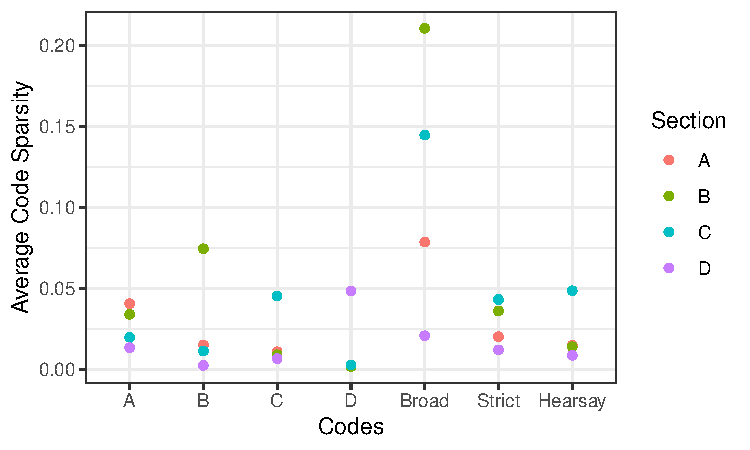
\includegraphics[width=  0.5 \linewidth]{sparsity_codes_sections}
	\end{figure}

\section{Correlation matrices}

\begin{landscape}
	\begin{figure}[H]
		\centering
		\caption{Correlation matrix at whole interview level} 
		\label{fig:cormat_whole}
		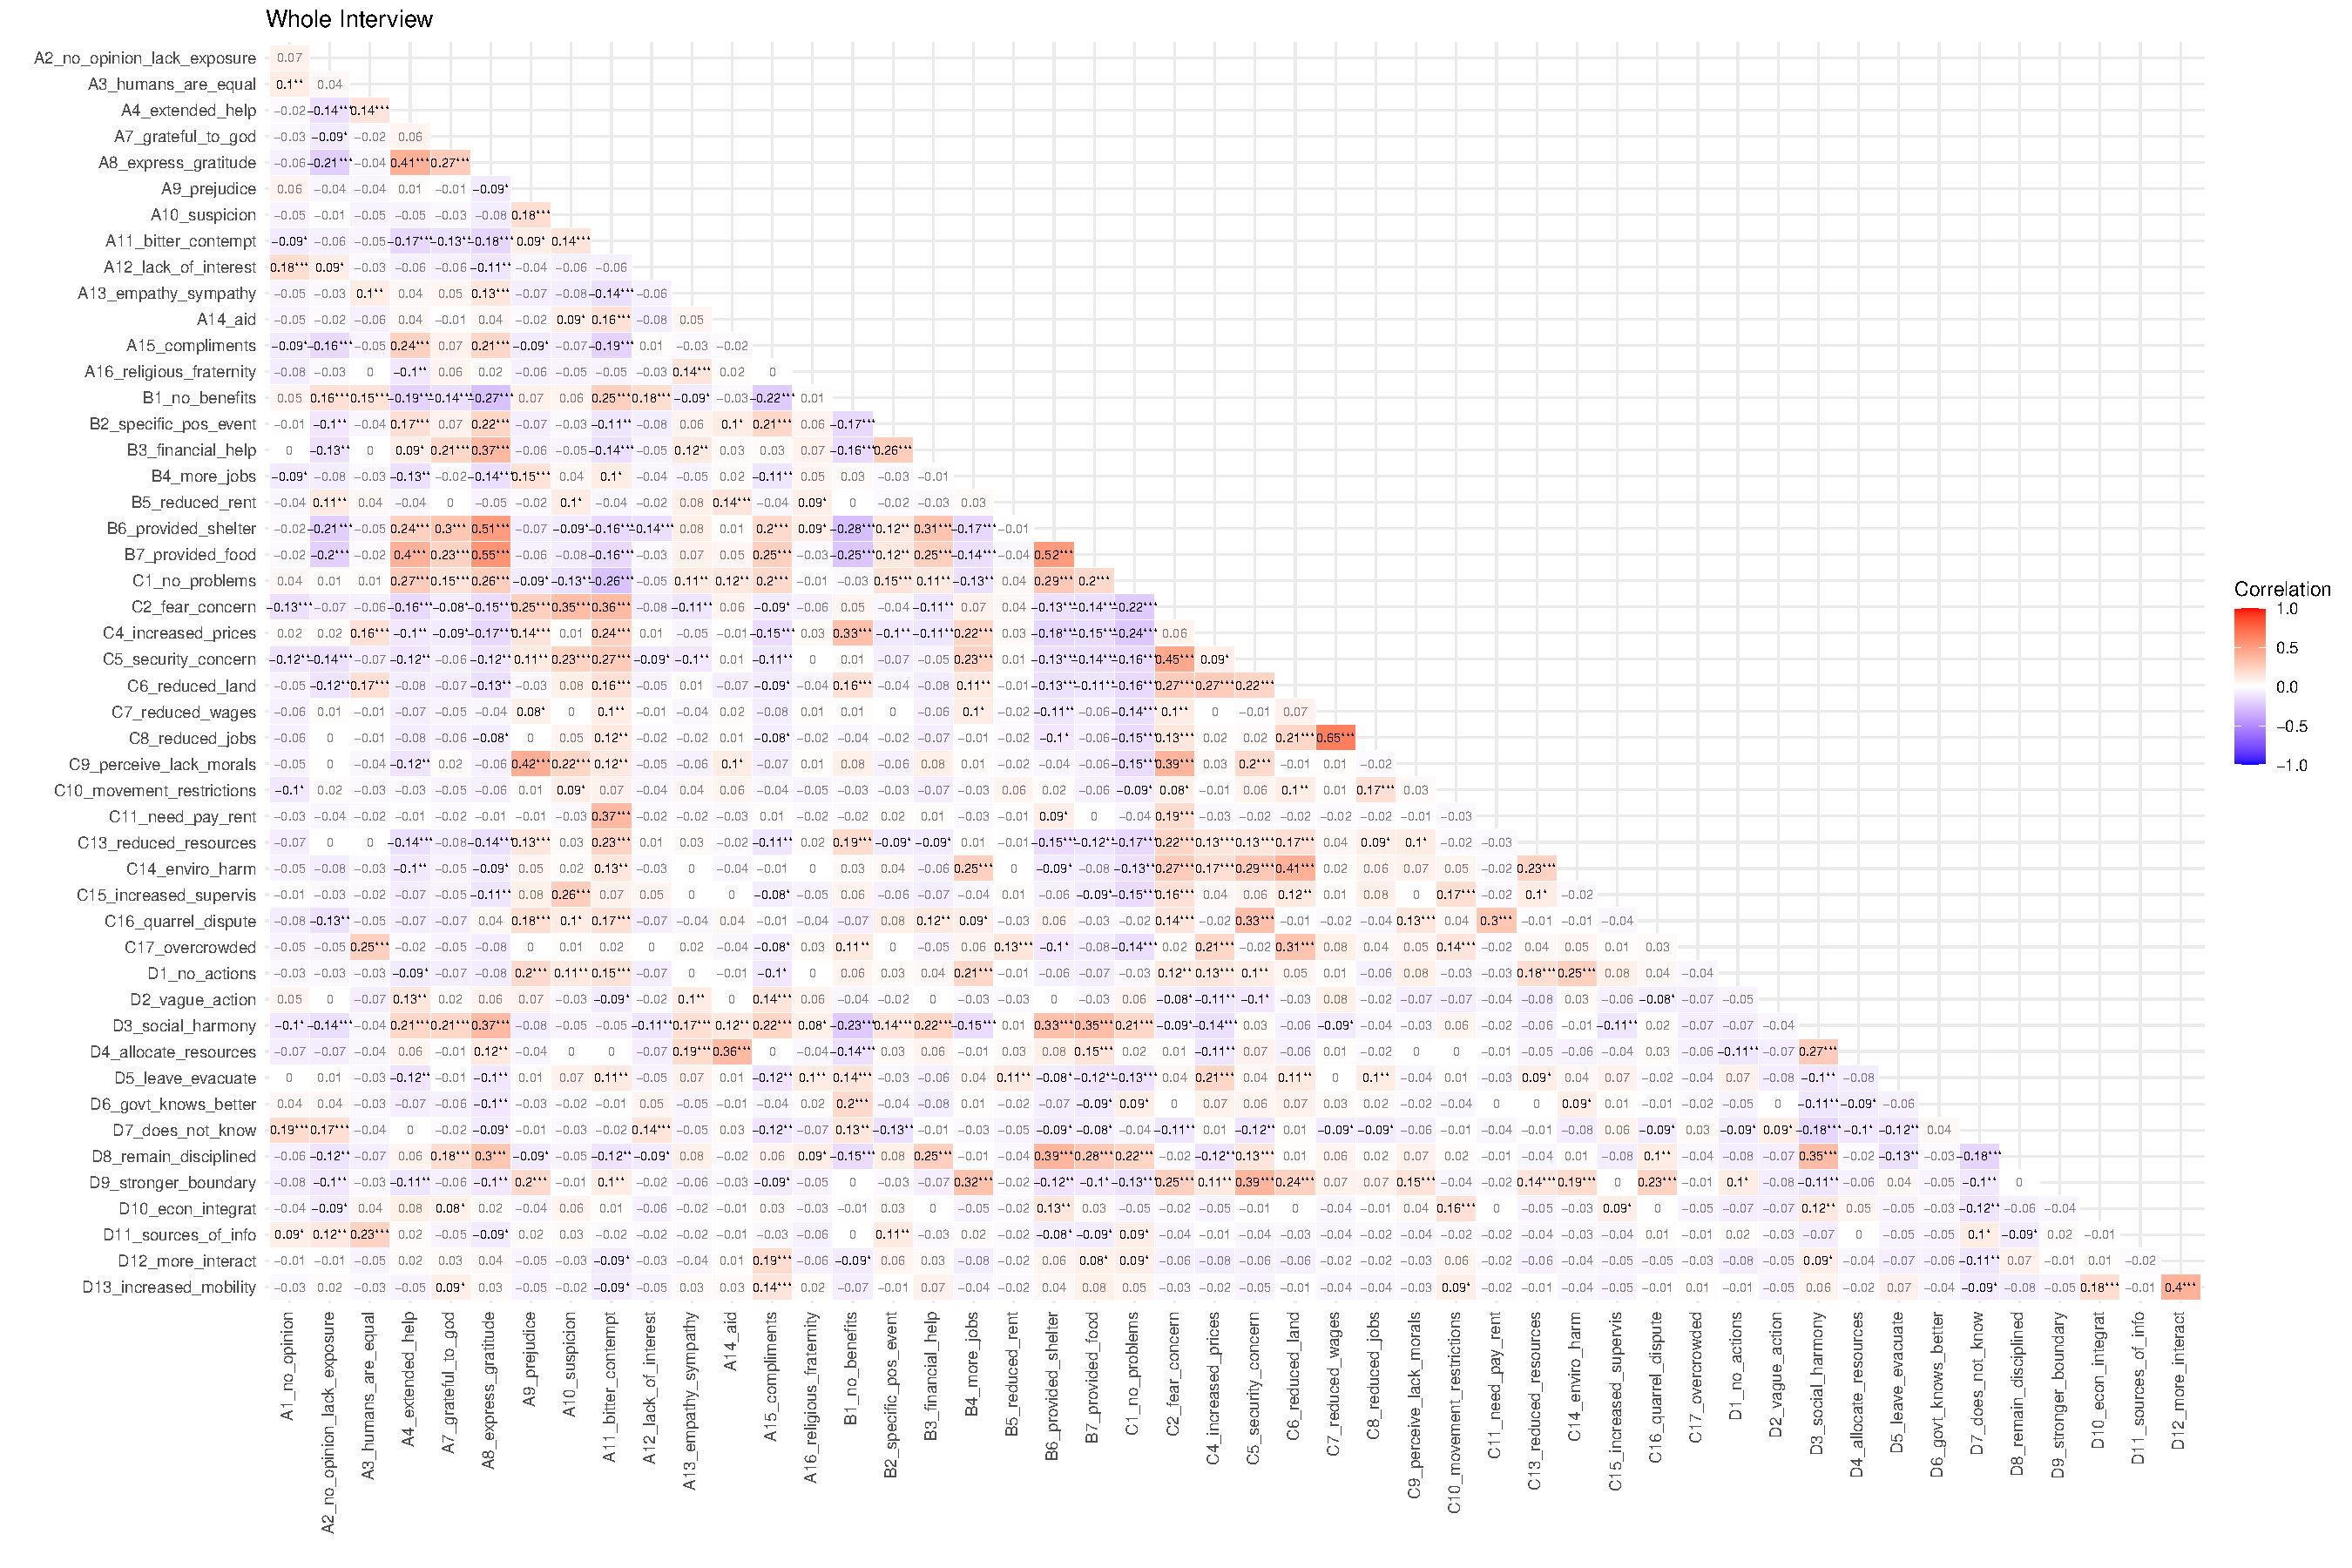
\includegraphics[width=  \linewidth]{cormat_whole}
	\end{figure}

	\begin{figure}[H]
		\centering
		\caption{Correlation matrix and Section level} 
		\label{fig:cormat_sec}
		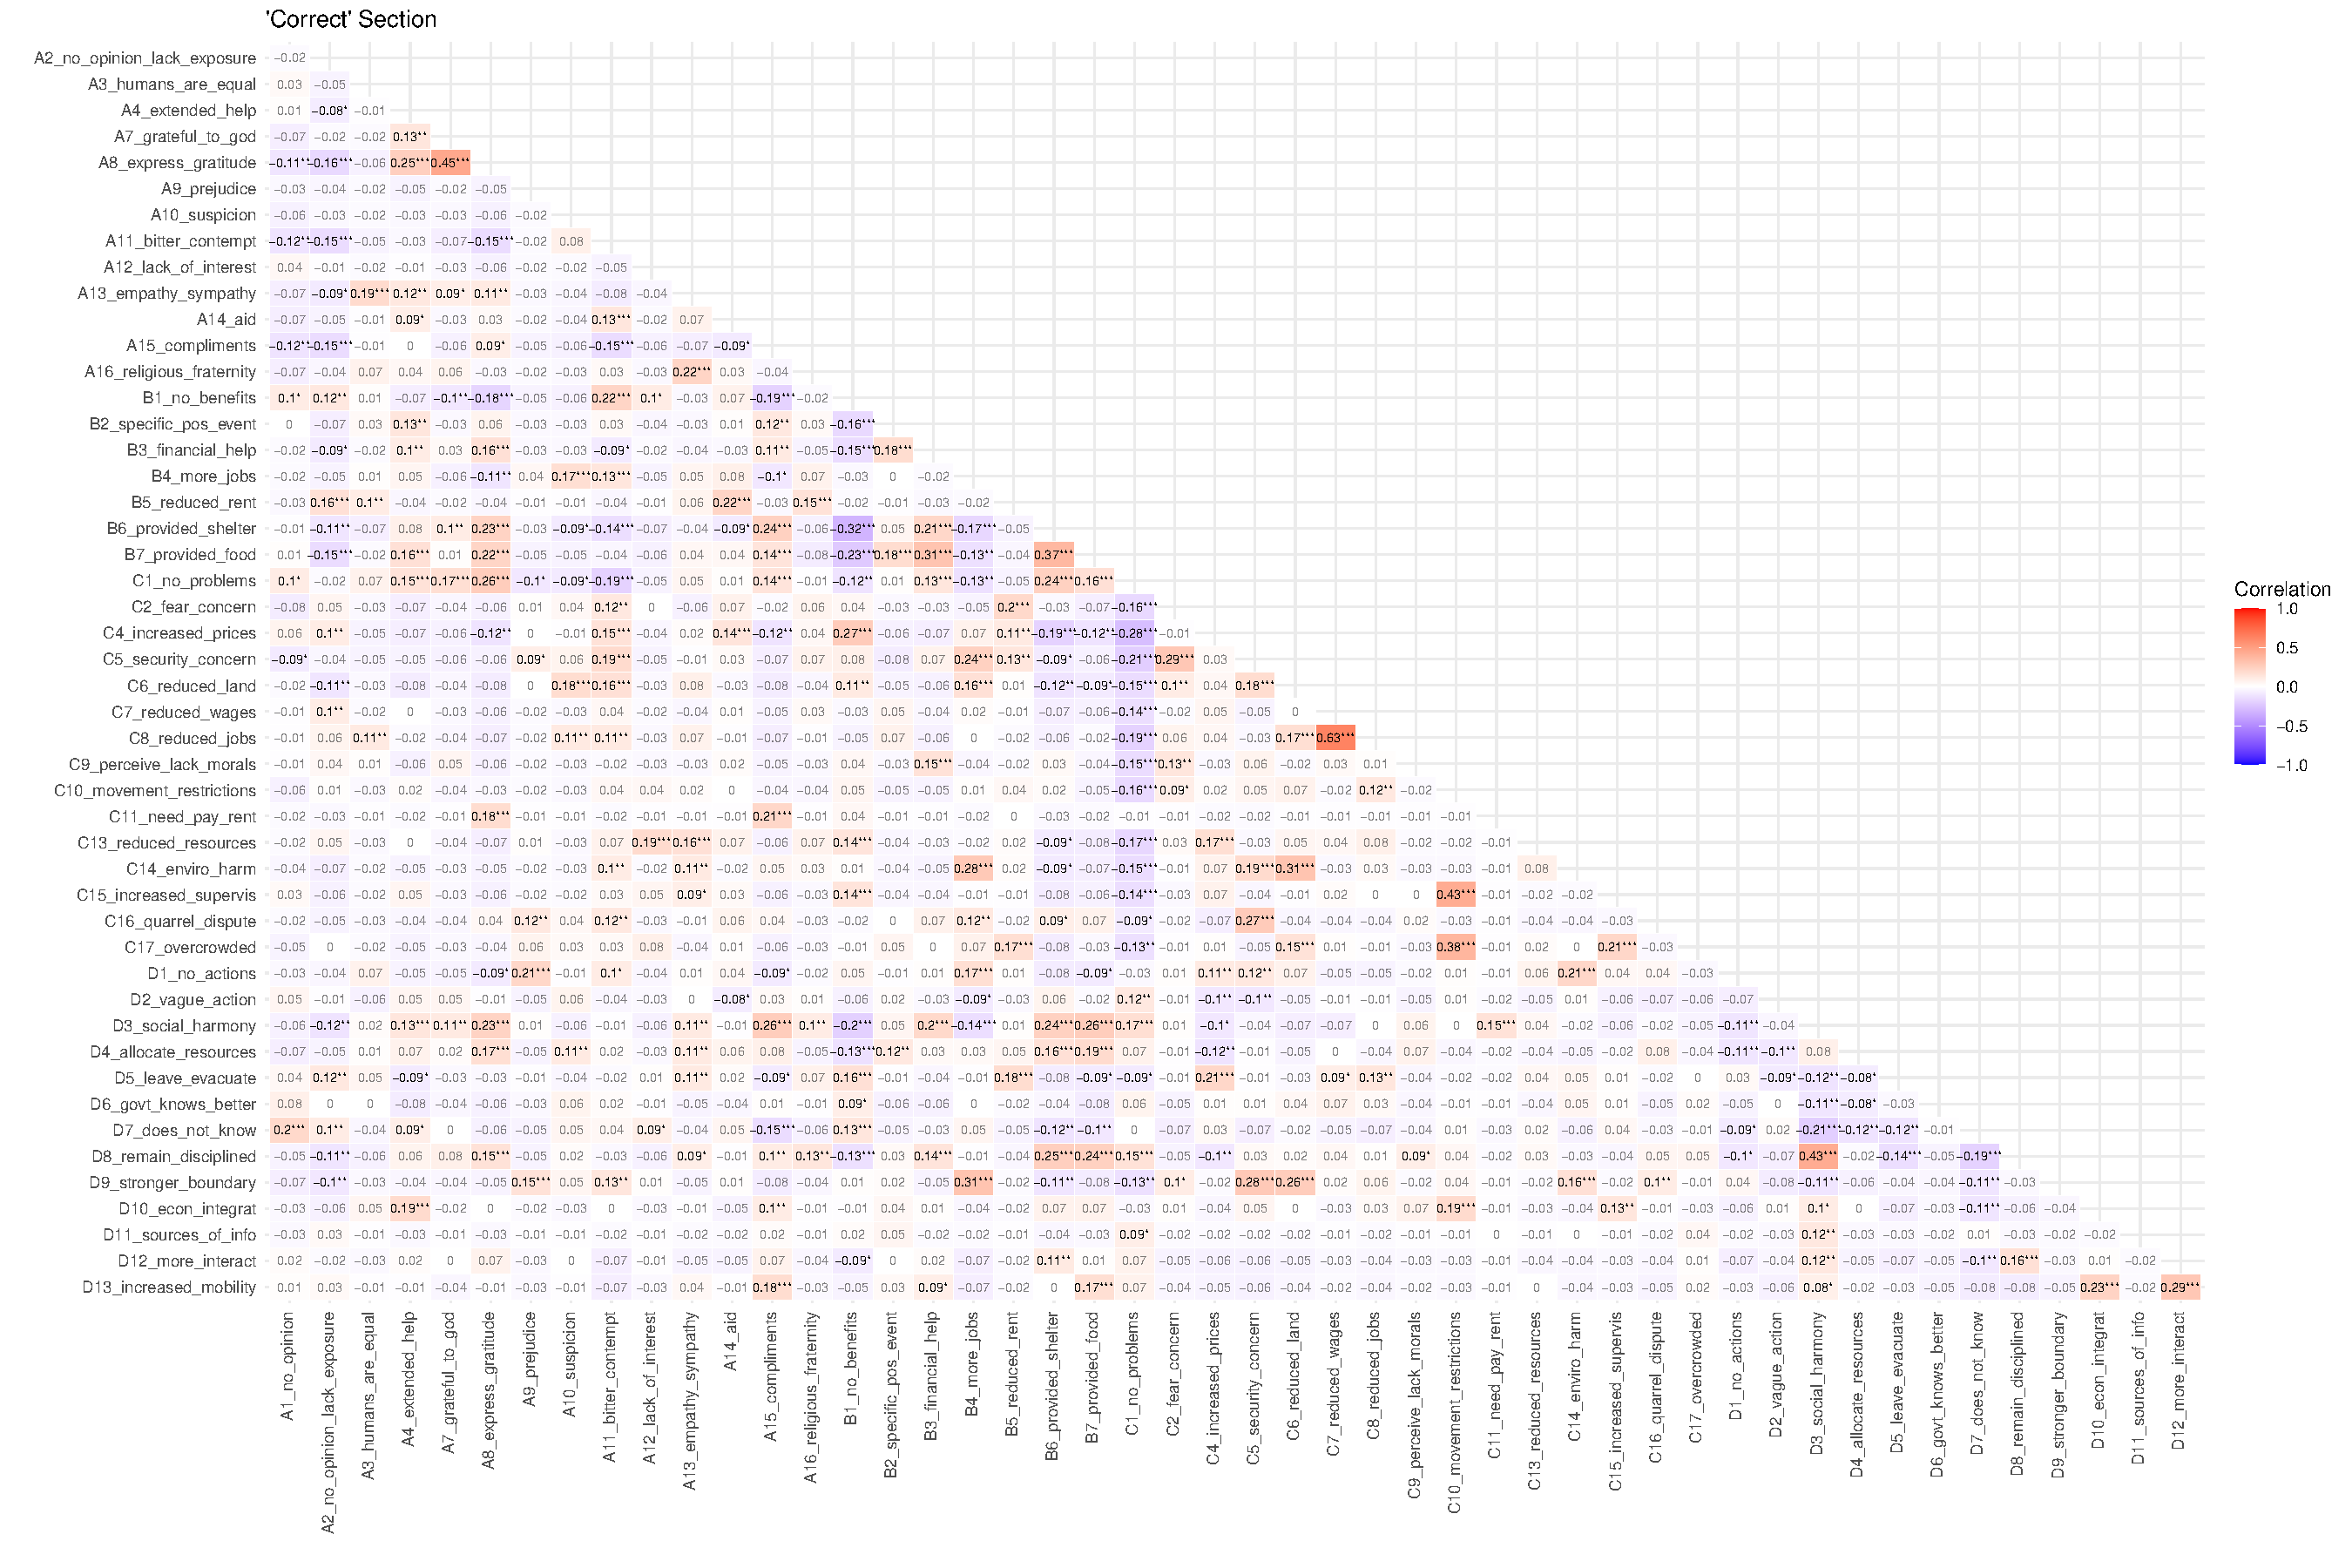
\includegraphics[width= \linewidth]{cormat_section}
	\end{figure}


\end{landscape}




\section{What explains the A codes?}


% Table created by stargazer v.5.2.3 by Marek Hlavac, Social Policy Institute. E-mail: marek.hlavac at gmail.com
% Date and time: Mon, Feb 27, 2023 - 13:15:30
\begin{table}[H] \centering 
  \caption{A1.no.opinion} 
  \label{} 
\tiny 
\begin{tabular}{@{\extracolsep{4pt}}lcccccccccc} 
\\[-1.8ex]\hline 
\hline \\[-1.8ex] 
 & \multicolumn{10}{c}{\textit{Dependent variable:}} \\ 
\cline{2-11} 
\\[-1.8ex] & \multicolumn{10}{c}{A1\_no\_opinion} \\ 
\\[-1.8ex] & (1) & (2) & (3) & (4) & (5) & (6) & (7) & (8) & (9) & (10)\\ 
\hline \\[-1.8ex] 
 strict\_direct\_exp &  &  &  & $-$0.055 & $-$0.038 &  &  &  & $-$0.165 & $-$0.026 \\ 
  &  &  &  & (0.058) & (0.088) &  &  &  & (0.183) & (0.312) \\ 
  & & & & & & & & & & \\ 
 broad\_direct\_exp &  &  &  & $-$0.016 & 0.012 &  &  &  & $-$0.091 & $-$0.047 \\ 
  &  &  &  & (0.027) & (0.036) &  &  &  & (0.080) & (0.124) \\ 
  & & & & & & & & & & \\ 
 hearsay &  &  &  & 0.007 & $-$0.001 &  &  &  & 0.055 & 0.100 \\ 
  &  &  &  & (0.062) & (0.077) &  &  &  & (0.201) & (0.292) \\ 
  & & & & & & & & & & \\ 
 B1\_no\_benefits & 0.008 &  & $-$0.007 & $-$0.007 & $-$0.029 & 0.033 &  & 0.027 & 0.022 & 0.039 \\ 
  & (0.044) &  & (0.047) & (0.047) & (0.056) & (0.031) &  & (0.033) & (0.033) & (0.043) \\ 
  & & & & & & & & & & \\ 
 B2\_specific\_pos\_event & $-$0.004 &  & $-$0.016 & 0.001 & $-$0.075 & 0.011 &  & 0.003 & 0.012 & $-$0.015 \\ 
  & (0.060) &  & (0.061) & (0.065) & (0.149) & (0.065) &  & (0.066) & (0.069) & (0.147) \\ 
  & & & & & & & & & & \\ 
 B3\_financial\_help & 0.026 &  & 0.017 & 0.015 & $-$0.148 & $-$0.025 &  & $-$0.026 & $-$0.028 & $-$0.094 \\ 
  & (0.080) &  & (0.082) & (0.082) & (0.261) & (0.063) &  & (0.066) & (0.066) & (0.214) \\ 
  & & & & & & & & & & \\ 
 B4\_more\_jobs & $-$0.099$^{*}$ &  & $-$0.099$^{*}$ & $-$0.094$^{*}$ & $-$0.079 & $-$0.025 &  & $-$0.0001 & $-$0.001 & 0.014 \\ 
  & (0.051) &  & (0.054) & (0.055) & (0.059) & (0.044) &  & (0.050) & (0.051) & (0.062) \\ 
  & & & & & & & & & & \\ 
 B5\_reduced\_rent & $-$0.236 &  & $-$0.225 & $-$0.219 & $-$0.349 & $-$0.200 &  & $-$0.071 & $-$0.066 & $-$0.031 \\ 
  & (0.265) &  & (0.270) & (0.271) & (0.280) & (0.251) &  & (0.268) & (0.269) & (0.322) \\ 
  & & & & & & & & & & \\ 
 B6\_provided\_shelter & 0.004 &  & 0.004 & 0.006 & 0.010 & 0.031 &  & 0.025 & 0.027 & 1.787$^{**}$ \\ 
  & (0.036) &  & (0.037) & (0.038) & (0.119) & (0.035) &  & (0.036) & (0.037) & (0.899) \\ 
  & & & & & & & & & & \\ 
 B7\_provided\_food & $-$0.002 &  & $-$0.015 & $-$0.007 & $-$0.262 & 0.042 &  & 0.034 & 0.044 &  \\ 
  & (0.046) &  & (0.046) & (0.048) & (0.738) & (0.046) &  & (0.047) & (0.048) &  \\ 
  & & & & & & & & & & \\ 
 C1\_no\_problems &  & 0.003 & 0.005 & 0.004 & 0.163$^{***}$ &  & 0.045$^{*}$ & 0.043 & 0.040 & 0.111$^{**}$ \\ 
  &  & (0.029) & (0.030) & (0.030) & (0.055) &  & (0.027) & (0.027) & (0.028) & (0.050) \\ 
  & & & & & & & & & & \\ 
 C2\_fear\_concern &  & $-$0.065 & $-$0.063 & $-$0.057 & $-$0.074 &  & $-$0.066 & $-$0.062 & $-$0.067 & $-$0.058 \\ 
  &  & (0.060) & (0.061) & (0.062) & (0.074) &  & (0.068) & (0.071) & (0.071) & (0.097) \\ 
  & & & & & & & & & & \\ 
 C4\_increased\_prices &  & 0.010 & 0.020 & 0.029 & 0.026 &  & 0.048 & 0.042 & 0.058 & 0.066 \\ 
  &  & (0.039) & (0.041) & (0.046) & (0.053) &  & (0.045) & (0.046) & (0.049) & (0.062) \\ 
  & & & & & & & & & & \\ 
 C5\_security\_concern &  & $-$0.056 & $-$0.050 & $-$0.047 & $-$0.037 &  & $-$0.070 & $-$0.067 & $-$0.067 & $-$0.041 \\ 
  &  & (0.038) & (0.039) & (0.041) & (0.048) &  & (0.053) & (0.054) & (0.056) & (0.076) \\ 
  & & & & & & & & & & \\ 
 C6\_reduced\_land &  & $-$0.017 & $-$0.027 & $-$0.009 & $-$0.024 &  & 0.004 & $-$0.003 & 0.015 & 0.003 \\ 
  &  & (0.087) & (0.088) & (0.090) & (0.093) &  & (0.068) & (0.069) & (0.070) & (0.086) \\ 
  & & & & & & & & & & \\ 
 C7\_reduced\_wages &  & $-$0.082 & $-$0.057 & $-$0.022 & $-$0.045 &  & $-$0.072 & $-$0.066 & $-$0.030 & $-$0.044 \\ 
  &  & (0.107) & (0.108) & (0.115) & (0.130) &  & (0.117) & (0.118) & (0.121) & (0.159) \\ 
  & & & & & & & & & & \\ 
 C8\_reduced\_jobs &  & $-$0.007 & $-$0.028 & $-$0.026 & 0.023 &  & 0.029 & 0.031 & 0.030 & 0.057 \\ 
  &  & (0.092) & (0.094) & (0.094) & (0.108) &  & (0.083) & (0.084) & (0.084) & (0.123) \\ 
  & & & & & & & & & & \\ 
 C9\_perceive\_lack\_morals &  & $-$0.008 & $-$0.020 & $-$0.015 & 0.104 &  & $-$0.003 & $-$0.003 & 0.006 & 0.075 \\ 
  &  & (0.073) & (0.075) & (0.076) & (0.095) &  & (0.094) & (0.097) & (0.098) & (0.155) \\ 
  & & & & & & & & & & \\ 
 C10\_movement\_restrictions &  & $-$0.116 & $-$0.116 & $-$0.100 & $-$0.156 &  & $-$0.077 & $-$0.084 & $-$0.067 & $-$0.081 \\ 
  &  & (0.079) & (0.080) & (0.081) & (0.108) &  & (0.083) & (0.084) & (0.085) & (0.118) \\ 
  & & & & & & & & & & \\ 
 C11\_need\_pay\_rent &  & $-$0.007 & $-$0.008 & 0.004 &  &  & $-$0.394 & $-$0.395 & $-$0.291 &  \\ 
  &  & (0.079) & (0.080) & (0.082) &  &  & (0.673) & (0.683) & (0.700) &  \\ 
  & & & & & & & & & & \\ 
 C13\_reduced\_resources &  & $-$0.104 & $-$0.121 & $-$0.121 & $-$0.112 &  & $-$0.068 & $-$0.073 & $-$0.076 & $-$0.036 \\ 
  &  & (0.074) & (0.075) & (0.076) & (0.078) &  & (0.089) & (0.090) & (0.091) & (0.108) \\ 
  & & & & & & & & & & \\ 
 C14\_enviro\_harm &  & 0.014 & 0.042 & 0.044 & 0.045 &  & $-$0.042 & $-$0.036 & $-$0.020 & $-$0.018 \\ 
  &  & (0.073) & (0.076) & (0.077) & (0.080) &  & (0.078) & (0.080) & (0.082) & (0.099) \\ 
  & & & & & & & & & & \\ 
 C15\_increased\_supervis &  & 0.014 & $-$0.005 & 0.024 & 0.084 &  & 0.073 & 0.066 & 0.078 & 0.110 \\ 
  &  & (0.093) & (0.094) & (0.098) & (0.106) &  & (0.089) & (0.090) & (0.091) & (0.111) \\ 
  & & & & & & & & & & \\ 
 C16\_quarrel\_dispute &  & $-$0.051 & $-$0.046 & $-$0.036 & $-$0.081 &  & 0.005 & $-$0.003 & 0.010 & $-$0.072 \\ 
  &  & (0.070) & (0.071) & (0.073) & (0.101) &  & (0.070) & (0.072) & (0.073) & (0.126) \\ 
  & & & & & & & & & & \\ 
 C17\_overcrowded &  & $-$0.091 & $-$0.077 & $-$0.086 & $-$0.030 &  & $-$0.100 & $-$0.080 & $-$0.087 & $-$0.041 \\ 
  &  & (0.101) & (0.103) & (0.104) & (0.109) &  & (0.114) & (0.119) & (0.120) & (0.152) \\ 
  & & & & & & & & & & \\ 
 refugee & $-$0.011 & $-$0.013 & $-$0.016$^{*}$ & $-$0.014 &  & $-$0.048 & $-$0.050$^{*}$ & $-$0.055 & $-$0.052 &  \\ 
  & (0.009) & (0.008) & (0.009) & (0.010) &  & (0.031) & (0.027) & (0.035) & (0.035) &  \\ 
  & & & & & & & & & & \\ 
 int\_sex & $-$0.0003 & $-$0.003 & $-$0.003 & $-$0.003 & 0.009 & 0.004 & 0.00004 & $-$0.0004 & $-$0.002 & 0.046 \\ 
  & (0.006) & (0.006) & (0.006) & (0.006) & (0.009) & (0.020) & (0.021) & (0.021) & (0.021) & (0.037) \\ 
  & & & & & & & & & & \\ 
 int\_age & $-$0.0003 & $-$0.0003 & $-$0.0002 & $-$0.0002 & 0.0001 & $-$0.001 & $-$0.0005 & $-$0.001 & $-$0.001 & 0.001 \\ 
  & (0.0003) & (0.0003) & (0.0003) & (0.0003) & (0.001) & (0.001) & (0.001) & (0.001) & (0.001) & (0.002) \\ 
  & & & & & & & & & & \\ 
 int\_eduyears & 0.0004 & 0.0005 & 0.0004 & 0.001 & 0.0002 & 0.0004 & 0.0003 & 0.0001 & 0.0005 & $-$0.0002 \\ 
  & (0.001) & (0.001) & (0.001) & (0.001) & (0.001) & (0.003) & (0.003) & (0.003) & (0.003) & (0.005) \\ 
  & & & & & & & & & & \\ 
 int\_reledu & 0.005 & 0.007 & 0.006 & 0.006 & $-$0.061 & 0.024 & 0.039 & 0.031 & 0.030 & $-$0.138 \\ 
  & (0.014) & (0.014) & (0.014) & (0.014) & (0.038) & (0.047) & (0.047) & (0.049) & (0.049) & (0.144) \\ 
  & & & & & & & & & & \\ 
 int\_trauma\_exp & $-$0.001 & $-$0.001 & $-$0.001 & $-$0.001 & $-$0.002 & $-$0.002 & $-$0.003 & $-$0.003 & $-$0.002 & $-$0.005 \\ 
  & (0.001) & (0.001) & (0.001) & (0.001) & (0.002) & (0.004) & (0.005) & (0.005) & (0.005) & (0.009) \\ 
  & & & & & & & & & & \\ 
 num\_child & $-$0.0004 & $-$0.0002 & $-$0.0004 & $-$0.0004 & 0.0005 & $-$0.001 & 0.0002 & $-$0.0001 & 0.00001 & 0.005 \\ 
  & (0.002) & (0.002) & (0.002) & (0.002) & (0.004) & (0.007) & (0.007) & (0.007) & (0.007) & (0.015) \\ 
  & & & & & & & & & & \\ 
 hh\_cons\_capita & $-$0.016 & 0.084 & 0.075 & 0.089 & 0.157 & 0.039 & 0.419 & 0.416 & 0.446 & 0.765 \\ 
  & (0.149) & (0.151) & (0.152) & (0.154) & (0.205) & (0.494) & (0.610) & (0.620) & (0.622) & (0.834) \\ 
  & & & & & & & & & & \\ 
 hh\_income & $-$0.001 & $-$0.001 & $-$0.001 & $-$0.001 & $-$0.001 & $-$0.005 & $-$0.006 & $-$0.006 & $-$0.006 & $-$0.007 \\ 
  & (0.002) & (0.002) & (0.002) & (0.002) & (0.002) & (0.005) & (0.005) & (0.005) & (0.006) & (0.007) \\ 
  & & & & & & & & & & \\ 
 distancekmfromcamps &  &  &  &  & 0.0002 &  &  &  &  & $-$0.0001 \\ 
  &  &  &  &  & (0.0002) &  &  &  &  & (0.001) \\ 
  & & & & & & & & & & \\ 
 Constant & 0.039$^{**}$ & 0.047$^{***}$ & 0.052$^{***}$ & 0.051$^{***}$ & 0.012 & 0.102$^{**}$ & 0.098$^{*}$ & 0.096$^{*}$ & 0.102$^{*}$ & $-$0.035 \\ 
  & (0.016) & (0.016) & (0.016) & (0.017) & (0.024) & (0.052) & (0.055) & (0.057) & (0.058) & (0.100) \\ 
  & & & & & & & & & & \\ 
\hline \\[-1.8ex] 
Observations & 386 & 386 & 386 & 386 & 195 & 380 & 372 & 371 & 371 & 188 \\ 
R$^{2}$ & 0.023 & 0.059 & 0.070 & 0.073 & 0.188 & 0.026 & 0.055 & 0.061 & 0.067 & 0.143 \\ 
Adjusted R$^{2}$ & $-$0.020 & $-$0.004 & $-$0.012 & $-$0.017 & 0.021 & $-$0.017 & $-$0.010 & $-$0.025 & $-$0.027 & $-$0.034 \\ 
Residual Std. Error & 0.056 & 0.056 & 0.056 & 0.056 & 0.055 & 0.185 & 0.186 & 0.188 & 0.188 & 0.217 \\ 
F Statistic & 0.532 & 0.943 & 0.859 & 0.815 & 1.127 & 0.601 & 0.847 & 0.708 & 0.709 & 0.808 \\ 
\hline 
\hline \\[-1.8ex] 
\textit{Note:}  & \multicolumn{10}{r}{$^{*}$p$<$0.1; $^{**}$p$<$0.05; $^{***}$p$<$0.01} \\ 
\end{tabular} 
\end{table} 
 
% Table created by stargazer v.5.2.3 by Marek Hlavac, Social Policy Institute. E-mail: marek.hlavac at gmail.com
% Date and time: Mon, Feb 27, 2023 - 13:15:33
\begin{table}[H] \centering 
  \caption{A2.no.opinion.lack.exposure} 
  \label{} 
\tiny 
\begin{tabular}{@{\extracolsep{4pt}}lcccccccccc} 
\\[-1.8ex]\hline 
\hline \\[-1.8ex] 
 & \multicolumn{10}{c}{\textit{Dependent variable:}} \\ 
\cline{2-11} 
\\[-1.8ex] & \multicolumn{10}{c}{A2\_no\_opinion\_lack\_exposure} \\ 
\\[-1.8ex] & (1) & (2) & (3) & (4) & (5) & (6) & (7) & (8) & (9) & (10)\\ 
\hline \\[-1.8ex] 
 strict\_direct\_exp &  &  &  & $-$0.127 & $-$0.013 &  &  &  & $-$0.409$^{*}$ & $-$0.264 \\ 
  &  &  &  & (0.085) & (0.159) &  &  &  & (0.233) & (0.393) \\ 
  & & & & & & & & & & \\ 
 broad\_direct\_exp &  &  &  & $-$0.051 & $-$0.042 &  &  &  & $-$0.222$^{**}$ & $-$0.201 \\ 
  &  &  &  & (0.040) & (0.064) &  &  &  & (0.102) & (0.156) \\ 
  & & & & & & & & & & \\ 
 hearsay &  &  &  & 0.028 & $-$0.041 &  &  &  & 0.121 & $-$0.074 \\ 
  &  &  &  & (0.091) & (0.138) &  &  &  & (0.256) & (0.367) \\ 
  & & & & & & & & & & \\ 
 B1\_no\_benefits & 0.034 &  & 0.013 & 0.009 & $-$0.098 & 0.009 &  & 0.034 & 0.022 & $-$0.006 \\ 
  & (0.067) &  & (0.069) & (0.070) & (0.101) & (0.041) &  & (0.043) & (0.043) & (0.054) \\ 
  & & & & & & & & & & \\ 
 B2\_specific\_pos\_event & $-$0.066 &  & $-$0.083 & $-$0.047 & $-$0.281 & $-$0.039 &  & $-$0.050 & $-$0.026 & 0.001 \\ 
  & (0.091) &  & (0.090) & (0.095) & (0.267) & (0.086) &  & (0.085) & (0.088) & (0.185) \\ 
  & & & & & & & & & & \\ 
 B3\_financial\_help & $-$0.006 &  & $-$0.004 & $-$0.004 & 0.554 & $-$0.009 &  & $-$0.002 & $-$0.006 & 0.091 \\ 
  & (0.122) &  & (0.121) & (0.121) & (0.467) & (0.083) &  & (0.085) & (0.084) & (0.269) \\ 
  & & & & & & & & & & \\ 
 B4\_more\_jobs & $-$0.278$^{***}$ &  & $-$0.238$^{***}$ & $-$0.224$^{***}$ & $-$0.239$^{**}$ & $-$0.123$^{**}$ &  & $-$0.067 & $-$0.069 & $-$0.057 \\ 
  & (0.077) &  & (0.080) & (0.081) & (0.105) & (0.059) &  & (0.064) & (0.065) & (0.078) \\ 
  & & & & & & & & & & \\ 
 B5\_reduced\_rent & 0.724$^{*}$ &  & 0.652 & 0.675$^{*}$ & 0.443 & 0.875$^{***}$ &  & 0.894$^{***}$ & 0.906$^{***}$ & 0.684$^{*}$ \\ 
  & (0.401) &  & (0.399) & (0.400) & (0.501) & (0.331) &  & (0.344) & (0.342) & (0.405) \\ 
  & & & & & & & & & & \\ 
 B6\_provided\_shelter & $-$0.067 &  & $-$0.072 & $-$0.066 & $-$0.158 & 0.010 &  & 0.003 & 0.007 & $-$0.657 \\ 
  & (0.055) &  & (0.055) & (0.056) & (0.213) & (0.046) &  & (0.046) & (0.047) & (1.131) \\ 
  & & & & & & & & & & \\ 
 B7\_provided\_food & $-$0.083 &  & $-$0.090 & $-$0.063 & $-$0.495 & $-$0.072 &  & $-$0.068 & $-$0.044 &  \\ 
  & (0.070) &  & (0.068) & (0.071) & (1.323) & (0.060) &  & (0.060) & (0.061) &  \\ 
  & & & & & & & & & & \\ 
 C1\_no\_problems &  & 0.045 & 0.053 & 0.052 & 0.128 &  & 0.013 & 0.010 & 0.003 & $-$0.003 \\ 
  &  & (0.043) & (0.044) & (0.044) & (0.099) &  & (0.035) & (0.035) & (0.035) & (0.062) \\ 
  & & & & & & & & & & \\ 
 C2\_fear\_concern &  & 0.039 & 0.001 & 0.016 & 0.048 &  & 0.078 & 0.015 & 0.002 & 0.034 \\ 
  &  & (0.091) & (0.091) & (0.091) & (0.133) &  & (0.089) & (0.091) & (0.091) & (0.122) \\ 
  & & & & & & & & & & \\ 
 C4\_increased\_prices &  & $-$0.023 & $-$0.004 & 0.028 & 0.054 &  & 0.046 & 0.022 & 0.059 & 0.068 \\ 
  &  & (0.059) & (0.060) & (0.068) & (0.094) &  & (0.058) & (0.059) & (0.063) & (0.079) \\ 
  & & & & & & & & & & \\ 
 C5\_security\_concern &  & $-$0.156$^{***}$ & $-$0.140$^{**}$ & $-$0.137$^{**}$ & $-$0.111 &  & $-$0.043 & $-$0.048 & $-$0.049 & $-$0.045 \\ 
  &  & (0.058) & (0.058) & (0.060) & (0.085) &  & (0.068) & (0.070) & (0.071) & (0.096) \\ 
  & & & & & & & & & & \\ 
 C6\_reduced\_land &  & $-$0.270$^{**}$ & $-$0.261$^{**}$ & $-$0.214 & $-$0.306$^{*}$ &  & $-$0.262$^{***}$ & $-$0.249$^{***}$ & $-$0.207$^{**}$ & $-$0.277$^{**}$ \\ 
  &  & (0.131) & (0.130) & (0.132) & (0.167) &  & (0.088) & (0.088) & (0.089) & (0.108) \\ 
  & & & & & & & & & & \\ 
 C7\_reduced\_wages &  & $-$0.125 & $-$0.049 & 0.048 & 0.086 &  & 0.095 & 0.098 & 0.186 & 0.171 \\ 
  &  & (0.161) & (0.160) & (0.169) & (0.233) &  & (0.152) & (0.152) & (0.154) & (0.200) \\ 
  & & & & & & & & & & \\ 
 C8\_reduced\_jobs &  & 0.032 & $-$0.011 & $-$0.004 & $-$0.006 &  & 0.042 & 0.058 & 0.055 & 0.121 \\ 
  &  & (0.139) & (0.139) & (0.139) & (0.194) &  & (0.108) & (0.108) & (0.107) & (0.154) \\ 
  & & & & & & & & & & \\ 
 C9\_perceive\_lack\_morals &  & 0.025 & 0.025 & 0.038 & $-$0.062 &  & 0.076 & 0.064 & 0.086 & 0.031 \\ 
  &  & (0.111) & (0.111) & (0.112) & (0.170) &  & (0.123) & (0.125) & (0.124) & (0.195) \\ 
  & & & & & & & & & & \\ 
 C10\_movement\_restrictions &  & 0.183 & 0.160 & 0.202$^{*}$ & 0.257 &  & 0.125 & 0.121 & 0.163 & 0.265$^{*}$ \\ 
  &  & (0.119) & (0.118) & (0.120) & (0.194) &  & (0.108) & (0.108) & (0.108) & (0.148) \\ 
  & & & & & & & & & & \\ 
 C11\_need\_pay\_rent &  & 0.021 & 0.027 & 0.053 &  &  & 0.182 & 0.135 & 0.392 &  \\ 
  &  & (0.120) & (0.118) & (0.121) &  &  & (0.876) & (0.877) & (0.890) &  \\ 
  & & & & & & & & & & \\ 
 C13\_reduced\_resources &  & $-$0.052 & $-$0.088 & $-$0.084 & $-$0.043 &  & $-$0.016 & $-$0.030 & $-$0.036 & $-$0.022 \\ 
  &  & (0.112) & (0.111) & (0.112) & (0.140) &  & (0.116) & (0.116) & (0.116) & (0.135) \\ 
  & & & & & & & & & & \\ 
 C14\_enviro\_harm &  & $-$0.104 & $-$0.021 & $-$0.009 & 0.034 &  & $-$0.096 & $-$0.066 & $-$0.027 & 0.013 \\ 
  &  & (0.110) & (0.112) & (0.114) & (0.144) &  & (0.101) & (0.103) & (0.104) & (0.125) \\ 
  & & & & & & & & & & \\ 
 C15\_increased\_supervis &  & $-$0.277$^{**}$ & $-$0.293$^{**}$ & $-$0.223 & $-$0.269 &  & $-$0.256$^{**}$ & $-$0.260$^{**}$ & $-$0.230$^{**}$ & $-$0.286$^{**}$ \\ 
  &  & (0.140) & (0.140) & (0.145) & (0.191) &  & (0.116) & (0.116) & (0.116) & (0.140) \\ 
  & & & & & & & & & & \\ 
 C16\_quarrel\_dispute &  & $-$0.138 & $-$0.096 & $-$0.072 & $-$0.043 &  & $-$0.064 & $-$0.041 & $-$0.007 & 0.063 \\ 
  &  & (0.106) & (0.105) & (0.107) & (0.181) &  & (0.091) & (0.092) & (0.092) & (0.159) \\ 
  & & & & & & & & & & \\ 
 C17\_overcrowded &  & $-$0.216 & $-$0.249 & $-$0.267$^{*}$ & $-$0.156 &  & $-$0.044 & $-$0.080 & $-$0.099 & $-$0.102 \\ 
  &  & (0.152) & (0.152) & (0.153) & (0.195) &  & (0.149) & (0.153) & (0.153) & (0.191) \\ 
  & & & & & & & & & & \\ 
 refugee & $-$0.040$^{***}$ & $-$0.070$^{***}$ & $-$0.059$^{***}$ & $-$0.056$^{***}$ &  & $-$0.115$^{***}$ & $-$0.136$^{***}$ & $-$0.115$^{***}$ & $-$0.109$^{**}$ &  \\ 
  & (0.013) & (0.012) & (0.014) & (0.014) &  & (0.040) & (0.036) & (0.044) & (0.044) &  \\ 
  & & & & & & & & & & \\ 
 int\_sex & 0.014 & 0.012 & 0.010 & 0.010 & 0.021 & 0.031 & 0.029 & 0.029 & 0.025 & 0.038 \\ 
  & (0.009) & (0.009) & (0.009) & (0.009) & (0.017) & (0.027) & (0.027) & (0.027) & (0.027) & (0.047) \\ 
  & & & & & & & & & & \\ 
 int\_age & $-$0.0001 & $-$0.0001 & $-$0.0001 & 0.00000 & $-$0.001 & $-$0.001 & $-$0.001 & $-$0.001 & $-$0.001 & $-$0.003 \\ 
  & (0.0005) & (0.0005) & (0.0005) & (0.0005) & (0.001) & (0.001) & (0.001) & (0.001) & (0.001) & (0.003) \\ 
  & & & & & & & & & & \\ 
 int\_eduyears & $-$0.001 & $-$0.0003 & $-$0.0004 & $-$0.0001 & $-$0.0004 & $-$0.002 & $-$0.002 & $-$0.002 & $-$0.001 & $-$0.003 \\ 
  & (0.001) & (0.001) & (0.001) & (0.001) & (0.002) & (0.004) & (0.004) & (0.004) & (0.004) & (0.006) \\ 
  & & & & & & & & & & \\ 
 int\_reledu & 0.006 & 0.009 & 0.010 & 0.009 & 0.116$^{*}$ & 0.028 & 0.014 & 0.029 & 0.026 & 0.308$^{*}$ \\ 
  & (0.021) & (0.021) & (0.021) & (0.021) & (0.068) & (0.062) & (0.062) & (0.063) & (0.062) & (0.181) \\ 
  & & & & & & & & & & \\ 
 int\_trauma\_exp & $-$0.002 & $-$0.001 & $-$0.002 & $-$0.002 & $-$0.003 & $-$0.010$^{*}$ & $-$0.012$^{**}$ & $-$0.013$^{**}$ & $-$0.012$^{**}$ & $-$0.030$^{**}$ \\ 
  & (0.002) & (0.002) & (0.002) & (0.002) & (0.004) & (0.006) & (0.006) & (0.006) & (0.006) & (0.012) \\ 
  & & & & & & & & & & \\ 
 num\_child & 0.0003 & $-$0.001 & $-$0.0001 & $-$0.0001 & 0.001 & $-$0.003 & $-$0.011 & $-$0.008 & $-$0.008 & $-$0.016 \\ 
  & (0.003) & (0.003) & (0.003) & (0.003) & (0.007) & (0.009) & (0.009) & (0.009) & (0.009) & (0.019) \\ 
  & & & & & & & & & & \\ 
 hh\_cons\_capita & $-$0.352 & $-$0.196 & $-$0.228 & $-$0.195 & $-$0.280 & $-$0.640 & $-$0.932 & $-$0.991 & $-$0.913 & $-$1.203 \\ 
  & (0.225) & (0.228) & (0.226) & (0.227) & (0.367) & (0.654) & (0.794) & (0.796) & (0.791) & (1.049) \\ 
  & & & & & & & & & & \\ 
 hh\_income & 0.004$^{*}$ & 0.004$^{*}$ & 0.005$^{**}$ & 0.004$^{*}$ & 0.006$^{*}$ & $-$0.002 & 0.001 & 0.001 & 0.0005 & 0.003 \\ 
  & (0.002) & (0.002) & (0.002) & (0.002) & (0.003) & (0.007) & (0.007) & (0.007) & (0.007) & (0.009) \\ 
  & & & & & & & & & & \\ 
 distancekmfromcamps &  &  &  &  & 0.001$^{*}$ &  &  &  &  & 0.002 \\ 
  &  &  &  &  & (0.0004) &  &  &  &  & (0.001) \\ 
  & & & & & & & & & & \\ 
 Constant & 0.086$^{***}$ & 0.098$^{***}$ & 0.102$^{***}$ & 0.100$^{***}$ & 0.093$^{**}$ & 0.264$^{***}$ & 0.313$^{***}$ & 0.290$^{***}$ & 0.303$^{***}$ & 0.372$^{***}$ \\ 
  & (0.024) & (0.024) & (0.024) & (0.024) & (0.044) & (0.068) & (0.072) & (0.074) & (0.074) & (0.126) \\ 
  & & & & & & & & & & \\ 
\hline \\[-1.8ex] 
Observations & 386 & 386 & 386 & 386 & 195 & 380 & 372 & 371 & 371 & 188 \\ 
R$^{2}$ & 0.141 & 0.180 & 0.221 & 0.229 & 0.261 & 0.108 & 0.135 & 0.162 & 0.182 & 0.247 \\ 
Adjusted R$^{2}$ & 0.104 & 0.126 & 0.153 & 0.154 & 0.110 & 0.069 & 0.075 & 0.085 & 0.099 & 0.091 \\ 
Residual Std. Error & 0.085 & 0.084 & 0.083 & 0.083 & 0.099 & 0.245 & 0.242 & 0.241 & 0.239 & 0.273 \\ 
F Statistic & 3.800$^{***}$ & 3.313$^{***}$ & 3.241$^{***}$ & 3.067$^{***}$ & 1.726$^{**}$ & 2.749$^{***}$ & 2.249$^{***}$ & 2.108$^{***}$ & 2.197$^{***}$ & 1.587$^{**}$ \\ 
\hline 
\hline \\[-1.8ex] 
\textit{Note:}  & \multicolumn{10}{r}{$^{*}$p$<$0.1; $^{**}$p$<$0.05; $^{***}$p$<$0.01} \\ 
\end{tabular} 
\end{table} 
 
% Table created by stargazer v.5.2.3 by Marek Hlavac, Social Policy Institute. E-mail: marek.hlavac at gmail.com
% Date and time: Mon, Feb 27, 2023 - 13:15:37
\begin{table}[H] \centering 
  \caption{A3.humans.are.equal} 
  \label{} 
\tiny 
\begin{tabular}{@{\extracolsep{4pt}}lcccccccccc} 
\\[-1.8ex]\hline 
\hline \\[-1.8ex] 
 & \multicolumn{10}{c}{\textit{Dependent variable:}} \\ 
\cline{2-11} 
\\[-1.8ex] & \multicolumn{10}{c}{A3\_humans\_are\_equal} \\ 
\\[-1.8ex] & (1) & (2) & (3) & (4) & (5) & (6) & (7) & (8) & (9) & (10)\\ 
\hline \\[-1.8ex] 
 strict\_direct\_exp &  &  &  & $-$0.012 & $-$0.020 &  &  &  & $-$0.034 & $-$0.071 \\ 
  &  &  &  & (0.031) & (0.053) &  &  &  & (0.038) & (0.072) \\ 
  & & & & & & & & & & \\ 
 broad\_direct\_exp &  &  &  & $-$0.004 & 0.010 &  &  &  & 0.007 & 0.023 \\ 
  &  &  &  & (0.015) & (0.021) &  &  &  & (0.017) & (0.029) \\ 
  & & & & & & & & & & \\ 
 hearsay &  &  &  & $-$0.014 & $-$0.019 &  &  &  & $-$0.045 & $-$0.043 \\ 
  &  &  &  & (0.033) & (0.046) &  &  &  & (0.042) & (0.067) \\ 
  & & & & & & & & & & \\ 
 B1\_no\_benefits & 0.056$^{**}$ &  & 0.030 & 0.029 & 0.012 & $-$0.006 &  & $-$0.003 & $-$0.003 & $-$0.0002 \\ 
  & (0.024) &  & (0.025) & (0.025) & (0.034) & (0.007) &  & (0.007) & (0.007) & (0.010) \\ 
  & & & & & & & & & & \\ 
 B2\_specific\_pos\_event & $-$0.025 &  & $-$0.033 & $-$0.026 & 0.028 & 0.005 &  & 0.002 & 0.007 & $-$0.015 \\ 
  & (0.033) &  & (0.033) & (0.034) & (0.089) & (0.014) &  & (0.014) & (0.014) & (0.034) \\ 
  & & & & & & & & & & \\ 
 B3\_financial\_help & 0.034 &  & 0.039 & 0.037 & $-$0.092 & $-$0.003 &  & $-$0.003 & $-$0.005 & $-$0.029 \\ 
  & (0.044) &  & (0.044) & (0.044) & (0.157) & (0.013) &  & (0.014) & (0.014) & (0.049) \\ 
  & & & & & & & & & & \\ 
 B4\_more\_jobs & $-$0.022 &  & $-$0.027 & $-$0.025 & $-$0.020 & $-$0.005 &  & 0.003 & 0.004 & 0.006 \\ 
  & (0.028) &  & (0.029) & (0.029) & (0.035) & (0.009) &  & (0.010) & (0.011) & (0.014) \\ 
  & & & & & & & & & & \\ 
 B5\_reduced\_rent & 0.152 &  & 0.083 & 0.085 & $-$0.013 & 0.102$^{*}$ &  & 0.139$^{**}$ & 0.135$^{**}$ & 0.154$^{**}$ \\ 
  & (0.146) &  & (0.144) & (0.145) & (0.168) & (0.053) &  & (0.056) & (0.056) & (0.074) \\ 
  & & & & & & & & & & \\ 
 B6\_provided\_shelter & $-$0.004 &  & $-$0.004 & $-$0.004 & 0.129$^{*}$ & $-$0.005 &  & $-$0.006 & $-$0.006 & $-$0.133 \\ 
  & (0.020) &  & (0.020) & (0.020) & (0.071) & (0.007) &  & (0.008) & (0.008) & (0.208) \\ 
  & & & & & & & & & & \\ 
 B7\_provided\_food & 0.0003 &  & $-$0.008 & $-$0.006 & $-$0.035 & 0.002 &  & 0.0002 & $-$0.002 &  \\ 
  & (0.025) &  & (0.025) & (0.026) & (0.443) & (0.010) &  & (0.010) & (0.010) &  \\ 
  & & & & & & & & & & \\ 
 C1\_no\_problems &  & 0.017 & 0.015 & 0.015 & 0.085$^{**}$ &  & 0.008 & 0.008 & 0.008 & 0.026$^{**}$ \\ 
  &  & (0.015) & (0.016) & (0.016) & (0.033) &  & (0.006) & (0.006) & (0.006) & (0.011) \\ 
  & & & & & & & & & & \\ 
 C2\_fear\_concern &  & $-$0.029 & $-$0.029 & $-$0.027 & $-$0.025 &  & $-$0.009 & $-$0.016 & $-$0.015 & $-$0.004 \\ 
  &  & (0.032) & (0.033) & (0.033) & (0.045) &  & (0.014) & (0.015) & (0.015) & (0.022) \\ 
  & & & & & & & & & & \\ 
 C4\_increased\_prices &  & 0.037$^{*}$ & 0.033 & 0.035 & 0.047 &  & $-$0.012 & $-$0.013 & $-$0.016 & $-$0.018 \\ 
  &  & (0.021) & (0.022) & (0.025) & (0.032) &  & (0.009) & (0.010) & (0.010) & (0.014) \\ 
  & & & & & & & & & & \\ 
 C5\_security\_concern &  & $-$0.010 & $-$0.008 & $-$0.004 & 0.012 &  & $-$0.006 & $-$0.009 & $-$0.006 & $-$0.003 \\ 
  &  & (0.021) & (0.021) & (0.022) & (0.029) &  & (0.011) & (0.011) & (0.012) & (0.018) \\ 
  & & & & & & & & & & \\ 
 C6\_reduced\_land &  & 0.130$^{***}$ & 0.125$^{***}$ & 0.129$^{***}$ & 0.129$^{**}$ &  & $-$0.017 & $-$0.013 & $-$0.013 & $-$0.013 \\ 
  &  & (0.046) & (0.047) & (0.048) & (0.056) &  & (0.014) & (0.014) & (0.015) & (0.020) \\ 
  & & & & & & & & & & \\ 
 C7\_reduced\_wages &  & 0.006 & 0.014 & 0.021 & 0.027 &  & $-$0.059$^{**}$ & $-$0.059$^{**}$ & $-$0.061$^{**}$ & $-$0.087$^{**}$ \\ 
  &  & (0.057) & (0.058) & (0.061) & (0.078) &  & (0.025) & (0.025) & (0.025) & (0.037) \\ 
  & & & & & & & & & & \\ 
 C8\_reduced\_jobs &  & $-$0.015 & $-$0.014 & $-$0.014 & $-$0.006 &  & 0.059$^{***}$ & 0.058$^{***}$ & 0.058$^{***}$ & 0.095$^{***}$ \\ 
  &  & (0.049) & (0.050) & (0.050) & (0.065) &  & (0.017) & (0.018) & (0.018) & (0.028) \\ 
  & & & & & & & & & & \\ 
 C9\_perceive\_lack\_morals &  & $-$0.019 & $-$0.029 & $-$0.026 & $-$0.109$^{*}$ &  & 0.013 & 0.018 & 0.018 & 0.010 \\ 
  &  & (0.039) & (0.040) & (0.041) & (0.057) &  & (0.020) & (0.020) & (0.020) & (0.036) \\ 
  & & & & & & & & & & \\ 
 C10\_movement\_restrictions &  & $-$0.039 & $-$0.042 & $-$0.040 & $-$0.084 &  & $-$0.014 & $-$0.011 & $-$0.012 & $-$0.012 \\ 
  &  & (0.042) & (0.042) & (0.043) & (0.065) &  & (0.017) & (0.018) & (0.018) & (0.027) \\ 
  & & & & & & & & & & \\ 
 C11\_need\_pay\_rent &  & 0.025 & 0.022 & 0.024 &  &  & $-$0.175 & $-$0.180 & $-$0.158 &  \\ 
  &  & (0.042) & (0.043) & (0.044) &  &  & (0.141) & (0.142) & (0.146) &  \\ 
  & & & & & & & & & & \\ 
 C13\_reduced\_resources &  & $-$0.002 & $-$0.012 & $-$0.011 & 0.018 &  & $-$0.013 & $-$0.011 & $-$0.011 & $-$0.009 \\ 
  &  & (0.040) & (0.040) & (0.041) & (0.047) &  & (0.019) & (0.019) & (0.019) & (0.025) \\ 
  & & & & & & & & & & \\ 
 C14\_enviro\_harm &  & $-$0.070$^{*}$ & $-$0.054 & $-$0.057 & $-$0.085$^{*}$ &  & $-$0.008 & $-$0.010 & $-$0.013 & $-$0.024 \\ 
  &  & (0.039) & (0.040) & (0.041) & (0.048) &  & (0.016) & (0.017) & (0.017) & (0.023) \\ 
  & & & & & & & & & & \\ 
 C15\_increased\_supervis &  & $-$0.029 & $-$0.031 & $-$0.024 & $-$0.041 &  & $-$0.004 & $-$0.001 & 0.0005 & 0.007 \\ 
  &  & (0.050) & (0.050) & (0.052) & (0.064) &  & (0.019) & (0.019) & (0.019) & (0.026) \\ 
  & & & & & & & & & & \\ 
 C16\_quarrel\_dispute &  & $-$0.035 & $-$0.029 & $-$0.025 & $-$0.008 &  & $-$0.011 & $-$0.008 & $-$0.008 & $-$0.037 \\ 
  &  & (0.037) & (0.038) & (0.039) & (0.061) &  & (0.015) & (0.015) & (0.015) & (0.029) \\ 
  & & & & & & & & & & \\ 
 C17\_overcrowded &  & 0.194$^{***}$ & 0.193$^{***}$ & 0.191$^{***}$ & 0.226$^{***}$ &  & 0.006 & $-$0.008 & $-$0.011 & $-$0.011 \\ 
  &  & (0.054) & (0.055) & (0.055) & (0.065) &  & (0.024) & (0.025) & (0.025) & (0.035) \\ 
  & & & & & & & & & & \\ 
 refugee & 0.001 & 0.00000 & 0.002 & 0.002 &  & $-$0.001 & $-$0.005 & $-$0.003 & $-$0.004 &  \\ 
  & (0.005) & (0.004) & (0.005) & (0.005) &  & (0.006) & (0.006) & (0.007) & (0.007) &  \\ 
  & & & & & & & & & & \\ 
 int\_sex & 0.003 & 0.002 & 0.002 & 0.002 & 0.004 & 0.005 & 0.006 & 0.006 & 0.006 & 0.011 \\ 
  & (0.003) & (0.003) & (0.003) & (0.003) & (0.006) & (0.004) & (0.004) & (0.004) & (0.004) & (0.009) \\ 
  & & & & & & & & & & \\ 
 int\_age & 0.001$^{***}$ & 0.001$^{***}$ & 0.001$^{***}$ & 0.001$^{***}$ & 0.001$^{**}$ & 0.001$^{***}$ & 0.001$^{**}$ & 0.001$^{**}$ & 0.001$^{**}$ & 0.001$^{***}$ \\ 
  & (0.0002) & (0.0002) & (0.0002) & (0.0002) & (0.0003) & (0.0002) & (0.0002) & (0.0002) & (0.0002) & (0.0005) \\ 
  & & & & & & & & & & \\ 
 int\_eduyears & 0.0004 & 0.0001 & 0.0001 & 0.0002 & 0.001 & 0.001$^{*}$ & 0.001 & 0.001$^{*}$ & 0.001$^{*}$ & 0.003$^{**}$ \\ 
  & (0.0005) & (0.0005) & (0.0005) & (0.0005) & (0.001) & (0.001) & (0.001) & (0.001) & (0.001) & (0.001) \\ 
  & & & & & & & & & & \\ 
 int\_reledu & 0.026$^{***}$ & 0.027$^{***}$ & 0.027$^{***}$ & 0.027$^{***}$ & 0.121$^{***}$ & 0.007 & 0.007 & 0.008 & 0.008 & $-$0.0002 \\ 
  & (0.008) & (0.008) & (0.008) & (0.008) & (0.023) & (0.010) & (0.010) & (0.010) & (0.010) & (0.033) \\ 
  & & & & & & & & & & \\ 
 int\_trauma\_exp & 0.00004 & $-$0.00003 & $-$0.0001 & $-$0.0001 & 0.001 & 0.00003 & 0.00004 & 0.0001 & 0.0001 & 0.002 \\ 
  & (0.001) & (0.001) & (0.001) & (0.001) & (0.001) & (0.001) & (0.001) & (0.001) & (0.001) & (0.002) \\ 
  & & & & & & & & & & \\ 
 num\_child & $-$0.001 & $-$0.002 & $-$0.001 & $-$0.001 & $-$0.004$^{*}$ & $-$0.001 & $-$0.002 & $-$0.002 & $-$0.002 & $-$0.004 \\ 
  & (0.001) & (0.001) & (0.001) & (0.001) & (0.002) & (0.001) & (0.002) & (0.002) & (0.002) & (0.003) \\ 
  & & & & & & & & & & \\ 
 hh\_cons\_capita & 0.039 & 0.075 & 0.069 & 0.071 & 0.156 & 0.197$^{*}$ & 0.277$^{**}$ & 0.287$^{**}$ & 0.294$^{**}$ & 0.414$^{**}$ \\ 
  & (0.082) & (0.081) & (0.081) & (0.082) & (0.123) & (0.105) & (0.128) & (0.129) & (0.130) & (0.193) \\ 
  & & & & & & & & & & \\ 
 hh\_income & $-$0.001 & $-$0.001 & $-$0.001 & $-$0.001 & $-$0.001 & $-$0.001 & $-$0.002 & $-$0.002 & $-$0.002 & $-$0.003$^{*}$ \\ 
  & (0.001) & (0.001) & (0.001) & (0.001) & (0.001) & (0.001) & (0.001) & (0.001) & (0.001) & (0.002) \\ 
  & & & & & & & & & & \\ 
 distancekmfromcamps &  &  &  &  & $-$0.00005 &  &  &  &  & $-$0.0003 \\ 
  &  &  &  &  & (0.0001) &  &  &  &  & (0.0002) \\ 
  & & & & & & & & & & \\ 
 Constant & $-$0.016$^{*}$ & $-$0.013 & $-$0.014$^{*}$ & $-$0.014 & $-$0.029$^{*}$ & $-$0.018 & $-$0.017 & $-$0.019 & $-$0.017 & $-$0.054$^{**}$ \\ 
  & (0.009) & (0.008) & (0.009) & (0.009) & (0.015) & (0.011) & (0.012) & (0.012) & (0.012) & (0.023) \\ 
  & & & & & & & & & & \\ 
\hline \\[-1.8ex] 
Observations & 386 & 386 & 386 & 386 & 195 & 380 & 372 & 371 & 371 & 188 \\ 
R$^{2}$ & 0.075 & 0.161 & 0.172 & 0.173 & 0.357 & 0.052 & 0.098 & 0.117 & 0.123 & 0.221 \\ 
Adjusted R$^{2}$ & 0.035 & 0.105 & 0.099 & 0.093 & 0.226 & 0.011 & 0.035 & 0.036 & 0.034 & 0.060 \\ 
Residual Std. Error & 0.031 & 0.030 & 0.030 & 0.030 & 0.033 & 0.039 & 0.039 & 0.039 & 0.039 & 0.050 \\ 
F Statistic & 1.878$^{**}$ & 2.888$^{***}$ & 2.371$^{***}$ & 2.159$^{***}$ & 2.713$^{***}$ & 1.254 & 1.564$^{**}$ & 1.443$^{*}$ & 1.385$^{*}$ & 1.372 \\ 
\hline 
\hline \\[-1.8ex] 
\textit{Note:}  & \multicolumn{10}{r}{$^{*}$p$<$0.1; $^{**}$p$<$0.05; $^{***}$p$<$0.01} \\ 
\end{tabular} 
\end{table} 
 
% Table created by stargazer v.5.2.3 by Marek Hlavac, Social Policy Institute. E-mail: marek.hlavac at gmail.com
% Date and time: Mon, Feb 27, 2023 - 13:15:41
\begin{table}[H] \centering 
  \caption{A4.extended.help} 
  \label{} 
\tiny 
\begin{tabular}{@{\extracolsep{4pt}}lcccccccccc} 
\\[-1.8ex]\hline 
\hline \\[-1.8ex] 
 & \multicolumn{10}{c}{\textit{Dependent variable:}} \\ 
\cline{2-11} 
\\[-1.8ex] & \multicolumn{10}{c}{A4\_extended\_help} \\ 
\\[-1.8ex] & (1) & (2) & (3) & (4) & (5) & (6) & (7) & (8) & (9) & (10)\\ 
\hline \\[-1.8ex] 
 strict\_direct\_exp &  &  &  & $-$0.122 & 0.061 &  &  &  & 0.289 & 0.541$^{**}$ \\ 
  &  &  &  & (0.098) & (0.105) &  &  &  & (0.215) & (0.269) \\ 
  & & & & & & & & & & \\ 
 broad\_direct\_exp &  &  &  & 0.039 & 0.014 &  &  &  & $-$0.019 & $-$0.090 \\ 
  &  &  &  & (0.046) & (0.042) &  &  &  & (0.095) & (0.107) \\ 
  & & & & & & & & & & \\ 
 hearsay &  &  &  & $-$0.134 & 0.063 &  &  &  & $-$0.295 & $-$0.148 \\ 
  &  &  &  & (0.104) & (0.091) &  &  &  & (0.237) & (0.251) \\ 
  & & & & & & & & & & \\ 
 B1\_no\_benefits & $-$0.045 &  & $-$0.112 & $-$0.099 & $-$0.061 & $-$0.011 &  & $-$0.019 & $-$0.018 & 0.001 \\ 
  & (0.075) &  & (0.079) & (0.080) & (0.067) & (0.037) &  & (0.039) & (0.039) & (0.037) \\ 
  & & & & & & & & & & \\ 
 B2\_specific\_pos\_event & 0.227$^{**}$ &  & 0.198$^{*}$ & 0.260$^{**}$ & 0.196 & 0.101 &  & 0.104 & 0.095 & 0.564$^{***}$ \\ 
  & (0.102) &  & (0.103) & (0.109) & (0.177) & (0.076) &  & (0.078) & (0.081) & (0.126) \\ 
  & & & & & & & & & & \\ 
 B3\_financial\_help & $-$0.148 &  & $-$0.120 & $-$0.153 & 0.392 & 0.066 &  & 0.067 & 0.067 & $-$0.216 \\ 
  & (0.136) &  & (0.138) & (0.139) & (0.309) & (0.074) &  & (0.077) & (0.078) & (0.184) \\ 
  & & & & & & & & & & \\ 
 B4\_more\_jobs & $-$0.067 &  & $-$0.063 & $-$0.063 & $-$0.088 & 0.053 &  & 0.101$^{*}$ & 0.115$^{*}$ & 0.128$^{**}$ \\ 
  & (0.086) &  & (0.092) & (0.093) & (0.070) & (0.052) &  & (0.059) & (0.060) & (0.053) \\ 
  & & & & & & & & & & \\ 
 B5\_reduced\_rent & $-$0.009 &  & $-$0.205 & $-$0.239 & $-$0.434 & $-$0.081 &  & 0.050 & 0.050 & $-$0.072 \\ 
  & (0.450) &  & (0.457) & (0.457) & (0.331) & (0.296) &  & (0.315) & (0.316) & (0.277) \\ 
  & & & & & & & & & & \\ 
 B6\_provided\_shelter & $-$0.025 &  & $-$0.056 & $-$0.072 & 0.415$^{***}$ & 0.008 &  & $-$0.005 & 0.004 & $-$0.677 \\ 
  & (0.062) &  & (0.063) & (0.064) & (0.141) & (0.041) &  & (0.043) & (0.043) & (0.774) \\ 
  & & & & & & & & & & \\ 
 B7\_provided\_food & 0.445$^{***}$ &  & 0.429$^{***}$ & 0.408$^{***}$ & 0.902 & 0.109$^{**}$ &  & 0.107$^{*}$ & 0.108$^{*}$ &  \\ 
  & (0.078) &  & (0.078) & (0.081) & (0.875) & (0.054) &  & (0.055) & (0.056) &  \\ 
  & & & & & & & & & & \\ 
 C1\_no\_problems &  & 0.178$^{***}$ & 0.171$^{***}$ & 0.170$^{***}$ & 0.146$^{**}$ &  & 0.073$^{**}$ & 0.060$^{*}$ & 0.061$^{*}$ & 0.079$^{*}$ \\ 
  &  & (0.051) & (0.051) & (0.050) & (0.065) &  & (0.032) & (0.032) & (0.032) & (0.043) \\ 
  & & & & & & & & & & \\ 
 C2\_fear\_concern &  & $-$0.101 & $-$0.082 & $-$0.069 & $-$0.023 &  & $-$0.054 & $-$0.030 & $-$0.021 & $-$0.002 \\ 
  &  & (0.107) & (0.104) & (0.105) & (0.088) &  & (0.084) & (0.084) & (0.084) & (0.083) \\ 
  & & & & & & & & & & \\ 
 C4\_increased\_prices &  & 0.025 & 0.057 & 0.012 & 0.044 &  & $-$0.049 & $-$0.049 & $-$0.044 & $-$0.008 \\ 
  &  & (0.069) & (0.069) & (0.078) & (0.062) &  & (0.055) & (0.054) & (0.058) & (0.054) \\ 
  & & & & & & & & & & \\ 
 C5\_security\_concern &  & 0.059 & 0.066 & 0.102 & 0.015 &  & 0.054 & 0.029 & 0.031 & 0.005 \\ 
  &  & (0.068) & (0.066) & (0.069) & (0.056) &  & (0.064) & (0.064) & (0.065) & (0.066) \\ 
  & & & & & & & & & & \\ 
 C6\_reduced\_land &  & 0.069 & 0.076 & 0.088 & 0.023 &  & $-$0.036 & $-$0.031 & $-$0.050 & $-$0.086 \\ 
  &  & (0.154) & (0.149) & (0.151) & (0.111) &  & (0.082) & (0.081) & (0.082) & (0.074) \\ 
  & & & & & & & & & & \\ 
 C7\_reduced\_wages &  & 0.087 & 0.086 & 0.061 & 0.006 &  & 0.040 & 0.040 & 0.026 & 0.009 \\ 
  &  & (0.189) & (0.183) & (0.193) & (0.154) &  & (0.143) & (0.139) & (0.143) & (0.137) \\ 
  & & & & & & & & & & \\ 
 C8\_reduced\_jobs &  & $-$0.063 & $-$0.109 & $-$0.112 & $-$0.025 &  & 0.008 & $-$0.015 & $-$0.023 & $-$0.001 \\ 
  &  & (0.163) & (0.159) & (0.159) & (0.128) &  & (0.101) & (0.099) & (0.099) & (0.106) \\ 
  & & & & & & & & & & \\ 
 C9\_perceive\_lack\_morals &  & $-$0.087 & $-$0.060 & $-$0.052 & $-$0.028 &  & $-$0.078 & $-$0.064 & $-$0.065 & 0.004 \\ 
  &  & (0.130) & (0.127) & (0.128) & (0.113) &  & (0.115) & (0.115) & (0.115) & (0.134) \\ 
  & & & & & & & & & & \\ 
 C10\_movement\_restrictions &  & $-$0.048 & 0.012 & 0.015 & $-$0.015 &  & 0.079 & 0.102 & 0.085 & 0.213$^{**}$ \\ 
  &  & (0.140) & (0.135) & (0.137) & (0.128) &  & (0.101) & (0.099) & (0.100) & (0.101) \\ 
  & & & & & & & & & & \\ 
 C11\_need\_pay\_rent &  & 0.051 & 0.079 & 0.111 &  &  & 0.282 & 0.362 & 0.106 &  \\ 
  &  & (0.141) & (0.136) & (0.138) &  &  & (0.822) & (0.804) & (0.822) &  \\ 
  & & & & & & & & & & \\ 
 C13\_reduced\_resources &  & $-$0.064 & $-$0.051 & $-$0.073 & $-$0.077 &  & 0.087 & 0.100 & 0.112 & 0.138 \\ 
  &  & (0.131) & (0.127) & (0.128) & (0.093) &  & (0.109) & (0.106) & (0.107) & (0.093) \\ 
  & & & & & & & & & & \\ 
 C14\_enviro\_harm &  & $-$0.108 & $-$0.146 & $-$0.196 & $-$0.126 &  & $-$0.067 & $-$0.106 & $-$0.112 & $-$0.052 \\ 
  &  & (0.130) & (0.128) & (0.130) & (0.095) &  & (0.095) & (0.095) & (0.096) & (0.085) \\ 
  & & & & & & & & & & \\ 
 C15\_increased\_supervis &  & 0.053 & 0.033 & 0.071 & $-$0.083 &  & 0.139 & 0.153 & 0.135 & 0.067 \\ 
  &  & (0.165) & (0.160) & (0.165) & (0.126) &  & (0.109) & (0.106) & (0.107) & (0.096) \\ 
  & & & & & & & & & & \\ 
 C16\_quarrel\_dispute &  & $-$0.186 & $-$0.185 & $-$0.167 & $-$0.143 &  & $-$0.056 & $-$0.081 & $-$0.079 & $-$0.048 \\ 
  &  & (0.124) & (0.121) & (0.122) & (0.120) &  & (0.086) & (0.084) & (0.085) & (0.109) \\ 
  & & & & & & & & & & \\ 
 C17\_overcrowded &  & 0.146 & 0.130 & 0.096 & 0.154 &  & $-$0.162 & $-$0.229 & $-$0.206 & $-$0.215 \\ 
  &  & (0.179) & (0.174) & (0.175) & (0.129) &  & (0.140) & (0.140) & (0.141) & (0.131) \\ 
  & & & & & & & & & & \\ 
 refugee & 0.036$^{**}$ & 0.064$^{***}$ & 0.030$^{*}$ & 0.031$^{*}$ &  & 0.002 & 0.019 & $-$0.007 & $-$0.016 &  \\ 
  & (0.015) & (0.014) & (0.016) & (0.016) &  & (0.036) & (0.033) & (0.041) & (0.041) &  \\ 
  & & & & & & & & & & \\ 
 int\_sex & 0.008 & 0.007 & 0.007 & 0.007 & 0.012 & 0.048$^{**}$ & 0.063$^{**}$ & 0.063$^{**}$ & 0.063$^{**}$ & 0.062$^{*}$ \\ 
  & (0.010) & (0.011) & (0.011) & (0.011) & (0.011) & (0.024) & (0.026) & (0.025) & (0.025) & (0.032) \\ 
  & & & & & & & & & & \\ 
 int\_age & 0.001$^{*}$ & 0.001$^{**}$ & 0.001$^{*}$ & 0.001$^{*}$ & 0.001$^{**}$ & 0.002 & 0.002 & 0.002 & 0.002 & 0.001 \\ 
  & (0.001) & (0.001) & (0.001) & (0.001) & (0.001) & (0.001) & (0.001) & (0.001) & (0.001) & (0.002) \\ 
  & & & & & & & & & & \\ 
 int\_eduyears & 0.002 & 0.002 & 0.002 & 0.002 & 0.003$^{*}$ & 0.008$^{**}$ & 0.008$^{**}$ & 0.008$^{**}$ & 0.008$^{**}$ & 0.004 \\ 
  & (0.001) & (0.002) & (0.001) & (0.001) & (0.002) & (0.003) & (0.004) & (0.003) & (0.003) & (0.004) \\ 
  & & & & & & & & & & \\ 
 int\_reledu & 0.001 & 0.018 & 0.010 & 0.005 & $-$0.003 & 0.012 & 0.050 & 0.029 & 0.032 & $-$0.022 \\ 
  & (0.024) & (0.025) & (0.024) & (0.024) & (0.045) & (0.056) & (0.058) & (0.057) & (0.057) & (0.124) \\ 
  & & & & & & & & & & \\ 
 int\_trauma\_exp & 0.003 & 0.002 & 0.002 & 0.002 & $-$0.0002 & 0.011$^{**}$ & 0.012$^{**}$ & 0.012$^{**}$ & 0.011$^{**}$ & $-$0.001 \\ 
  & (0.002) & (0.002) & (0.002) & (0.002) & (0.003) & (0.005) & (0.006) & (0.005) & (0.005) & (0.008) \\ 
  & & & & & & & & & & \\ 
 num\_child & 0.0003 & 0.0002 & $-$0.001 & $-$0.001 & $-$0.010$^{**}$ & 0.011 & 0.012 & 0.012 & 0.012 & $-$0.004 \\ 
  & (0.004) & (0.004) & (0.004) & (0.004) & (0.004) & (0.008) & (0.009) & (0.009) & (0.009) & (0.013) \\ 
  & & & & & & & & & & \\ 
 hh\_cons\_capita & $-$0.110 & 0.002 & $-$0.006 & 0.024 & $-$0.111 & $-$0.559 & $-$0.802 & $-$0.729 & $-$0.696 & $-$1.516$^{**}$ \\ 
  & (0.252) & (0.268) & (0.258) & (0.259) & (0.243) & (0.584) & (0.745) & (0.729) & (0.731) & (0.718) \\ 
  & & & & & & & & & & \\ 
 hh\_income & $-$0.0003 & $-$0.0005 & 0.00002 & $-$0.0003 & 0.0002 & $-$0.001 & 0.001 & 0.001 & 0.0003 & 0.002 \\ 
  & (0.003) & (0.003) & (0.003) & (0.003) & (0.002) & (0.006) & (0.007) & (0.006) & (0.006) & (0.006) \\ 
  & & & & & & & & & & \\ 
 distancekmfromcamps &  &  &  &  & 0.0002 &  &  &  &  & 0.001 \\ 
  &  &  &  &  & (0.0003) &  &  &  &  & (0.001) \\ 
  & & & & & & & & & & \\ 
 Constant & $-$0.015 & $-$0.036 & $-$0.021 & $-$0.020 & $-$0.026 & $-$0.090 & $-$0.127$^{*}$ & $-$0.122$^{*}$ & $-$0.115$^{*}$ & $-$0.036 \\ 
  & (0.027) & (0.028) & (0.028) & (0.028) & (0.029) & (0.061) & (0.067) & (0.067) & (0.068) & (0.086) \\ 
  & & & & & & & & & & \\ 
\hline \\[-1.8ex] 
Observations & 386 & 386 & 386 & 386 & 195 & 380 & 372 & 371 & 371 & 188 \\ 
R$^{2}$ & 0.214 & 0.173 & 0.256 & 0.265 & 0.245 & 0.080 & 0.089 & 0.122 & 0.130 & 0.291 \\ 
Adjusted R$^{2}$ & 0.179 & 0.118 & 0.191 & 0.194 & 0.090 & 0.040 & 0.026 & 0.042 & 0.042 & 0.145 \\ 
Residual Std. Error & 0.096 & 0.099 & 0.095 & 0.095 & 0.066 & 0.219 & 0.227 & 0.221 & 0.221 & 0.187 \\ 
F Statistic & 6.262$^{***}$ & 3.148$^{***}$ & 3.928$^{***}$ & 3.732$^{***}$ & 1.582$^{**}$ & 1.982$^{**}$ & 1.407$^{*}$ & 1.525$^{**}$ & 1.475$^{**}$ & 1.987$^{***}$ \\ 
\hline 
\hline \\[-1.8ex] 
\textit{Note:}  & \multicolumn{10}{r}{$^{*}$p$<$0.1; $^{**}$p$<$0.05; $^{***}$p$<$0.01} \\ 
\end{tabular} 
\end{table} 
 
% Table created by stargazer v.5.2.3 by Marek Hlavac, Social Policy Institute. E-mail: marek.hlavac at gmail.com
% Date and time: Mon, Feb 27, 2023 - 13:15:44
\begin{table}[H] \centering 
  \caption{A7.grateful.to.god} 
  \label{} 
\tiny 
\begin{tabular}{@{\extracolsep{4pt}}lcccccccccc} 
\\[-1.8ex]\hline 
\hline \\[-1.8ex] 
 & \multicolumn{10}{c}{\textit{Dependent variable:}} \\ 
\cline{2-11} 
\\[-1.8ex] & \multicolumn{10}{c}{A7\_grateful\_to\_god} \\ 
\\[-1.8ex] & (1) & (2) & (3) & (4) & (5) & (6) & (7) & (8) & (9) & (10)\\ 
\hline \\[-1.8ex] 
 strict\_direct\_exp &  &  &  & $-$0.002 & $-$0.028 &  &  &  & $-$0.030 & $-$0.009 \\ 
  &  &  &  & (0.045) & (0.019) &  &  &  & (0.128) & (0.010) \\ 
  & & & & & & & & & & \\ 
 broad\_direct\_exp &  &  &  & 0.003 & $-$0.010 &  &  &  & 0.052 & 0.0004 \\ 
  &  &  &  & (0.021) & (0.008) &  &  &  & (0.056) & (0.004) \\ 
  & & & & & & & & & & \\ 
 hearsay &  &  &  & $-$0.031 & $-$0.009 &  &  &  & $-$0.036 & 0.002 \\ 
  &  &  &  & (0.048) & (0.017) &  &  &  & (0.141) & (0.009) \\ 
  & & & & & & & & & & \\ 
 B1\_no\_benefits & $-$0.012 &  & $-$0.024 & $-$0.024 & 0.009 & $-$0.004 &  & $-$0.009 & $-$0.008 & 0.001 \\ 
  & (0.034) &  & (0.036) & (0.037) & (0.012) & (0.022) &  & (0.023) & (0.023) & (0.001) \\ 
  & & & & & & & & & & \\ 
 B2\_specific\_pos\_event & 0.001 &  & 0.008 & 0.014 & 0.076$^{**}$ & $-$0.031 &  & $-$0.025 & $-$0.019 & $-$0.003 \\ 
  & (0.046) &  & (0.047) & (0.050) & (0.033) & (0.045) &  & (0.046) & (0.048) & (0.005) \\ 
  & & & & & & & & & & \\ 
 B3\_financial\_help & 0.140$^{**}$ &  & 0.136$^{**}$ & 0.131$^{**}$ & 0.376$^{***}$ & 0.012 &  & $-$0.011 & $-$0.014 & 0.001 \\ 
  & (0.061) &  & (0.063) & (0.064) & (0.057) & (0.044) &  & (0.046) & (0.046) & (0.007) \\ 
  & & & & & & & & & & \\ 
 B4\_more\_jobs & 0.028 &  & 0.038 & 0.040 & 0.028$^{**}$ & $-$0.002 &  & 0.003 & 0.002 & 0.0003 \\ 
  & (0.039) &  & (0.042) & (0.043) & (0.013) & (0.031) &  & (0.035) & (0.036) & (0.002) \\ 
  & & & & & & & & & & \\ 
 B5\_reduced\_rent & 0.048 &  & 0.043 & 0.040 & 0.104$^{*}$ & 0.014 &  & 0.031 & 0.023 & 0.001 \\ 
  & (0.202) &  & (0.209) & (0.210) & (0.061) & (0.174) &  & (0.187) & (0.188) & (0.010) \\ 
  & & & & & & & & & & \\ 
 B6\_provided\_shelter & 0.088$^{***}$ &  & 0.087$^{***}$ & 0.086$^{***}$ & $-$0.032 & 0.001 &  & $-$0.009 & $-$0.012 & $-$0.003 \\ 
  & (0.028) &  & (0.029) & (0.029) & (0.026) & (0.024) &  & (0.025) & (0.026) & (0.028) \\ 
  & & & & & & & & & & \\ 
 B7\_provided\_food & 0.051 &  & 0.044 & 0.042 & 0.654$^{***}$ & $-$0.030 &  & $-$0.030 & $-$0.036 &  \\ 
  & (0.035) &  & (0.036) & (0.037) & (0.162) & (0.032) &  & (0.033) & (0.034) &  \\ 
  & & & & & & & & & & \\ 
 C1\_no\_problems &  & 0.036 & 0.023 & 0.023 & $-$0.006 &  & 0.043$^{**}$ & 0.046$^{**}$ & 0.046$^{**}$ & 0.002 \\ 
  &  & (0.023) & (0.023) & (0.023) & (0.012) &  & (0.019) & (0.019) & (0.019) & (0.002) \\ 
  & & & & & & & & & & \\ 
 C2\_fear\_concern &  & $-$0.068 & $-$0.040 & $-$0.039 & $-$0.007 &  & $-$0.014 & $-$0.017 & $-$0.015 & 0.001 \\ 
  &  & (0.048) & (0.048) & (0.048) & (0.016) &  & (0.048) & (0.050) & (0.050) & (0.003) \\ 
  & & & & & & & & & & \\ 
 C4\_increased\_prices &  & $-$0.004 & $-$0.004 & $-$0.008 & $-$0.0003 &  & 0.015 & 0.018 & 0.006 & $-$0.001 \\ 
  &  & (0.031) & (0.031) & (0.036) & (0.012) &  & (0.031) & (0.032) & (0.035) & (0.002) \\ 
  & & & & & & & & & & \\ 
 C5\_security\_concern &  & 0.022 & 0.017 & 0.023 & 0.007 &  & 0.003 & 0.003 & 0.008 & $-$0.001 \\ 
  &  & (0.031) & (0.030) & (0.032) & (0.010) &  & (0.037) & (0.038) & (0.039) & (0.002) \\ 
  & & & & & & & & & & \\ 
 C6\_reduced\_land &  & 0.020 & 0.021 & 0.021 & 0.012 &  & 0.013 & 0.014 & 0.011 & 0.001 \\ 
  &  & (0.069) & (0.068) & (0.070) & (0.021) &  & (0.047) & (0.048) & (0.049) & (0.003) \\ 
  & & & & & & & & & & \\ 
 C7\_reduced\_wages &  & $-$0.002 & $-$0.008 & $-$0.014 & 0.001 &  & 0.007 & 0.005 & $-$0.011 & 0.001 \\ 
  &  & (0.085) & (0.084) & (0.089) & (0.029) &  & (0.082) & (0.083) & (0.085) & (0.005) \\ 
  & & & & & & & & & & \\ 
 C8\_reduced\_jobs &  & $-$0.010 & $-$0.009 & $-$0.011 & 0.006 &  & $-$0.011 & $-$0.007 & $-$0.005 & 0.001 \\ 
  &  & (0.074) & (0.073) & (0.073) & (0.024) &  & (0.058) & (0.059) & (0.059) & (0.004) \\ 
  & & & & & & & & & & \\ 
 C9\_perceive\_lack\_morals &  & 0.100$^{*}$ & 0.080 & 0.082 & 0.008 &  & 0.117$^{*}$ & 0.118$^{*}$ & 0.116$^{*}$ & $-$0.0003 \\ 
  &  & (0.059) & (0.058) & (0.059) & (0.021) &  & (0.066) & (0.068) & (0.068) & (0.005) \\ 
  & & & & & & & & & & \\ 
 C10\_movement\_restrictions &  & $-$0.048 & $-$0.038 & $-$0.042 & 0.014 &  & $-$0.010 & $-$0.012 & $-$0.018 & $-$0.001 \\ 
  &  & (0.063) & (0.062) & (0.063) & (0.024) &  & (0.058) & (0.059) & (0.060) & (0.004) \\ 
  & & & & & & & & & & \\ 
 C11\_need\_pay\_rent &  & 0.008 & $-$0.001 & $-$0.002 &  &  & $-$0.218 & $-$0.246 & $-$0.212 &  \\ 
  &  & (0.063) & (0.062) & (0.064) &  &  & (0.471) & (0.478) & (0.490) &  \\ 
  & & & & & & & & & & \\ 
 C13\_reduced\_resources &  & $-$0.002 & 0.010 & 0.010 & 0.003 &  & 0.021 & 0.024 & 0.023 & $-$0.001 \\ 
  &  & (0.059) & (0.058) & (0.059) & (0.017) &  & (0.062) & (0.063) & (0.064) & (0.003) \\ 
  & & & & & & & & & & \\ 
 C14\_enviro\_harm &  & 0.012 & $-$0.017 & $-$0.024 & $-$0.010 &  & 0.018 & 0.015 & 0.005 & $-$0.001 \\ 
  &  & (0.059) & (0.058) & (0.060) & (0.018) &  & (0.054) & (0.056) & (0.057) & (0.003) \\ 
  & & & & & & & & & & \\ 
 C15\_increased\_supervis &  & 0.033 & 0.015 & 0.016 & 0.035 &  & 0.022 & 0.025 & 0.026 & 0.001 \\ 
  &  & (0.075) & (0.073) & (0.076) & (0.023) &  & (0.062) & (0.063) & (0.064) & (0.004) \\ 
  & & & & & & & & & & \\ 
 C16\_quarrel\_dispute &  & $-$0.084 & $-$0.108$^{*}$ & $-$0.105$^{*}$ & $-$0.001 &  & $-$0.021 & $-$0.016 & $-$0.022 & 0.0002 \\ 
  &  & (0.056) & (0.055) & (0.056) & (0.022) &  & (0.049) & (0.050) & (0.051) & (0.004) \\ 
  & & & & & & & & & & \\ 
 C17\_overcrowded &  & 0.002 & 0.0004 & $-$0.001 & $-$0.010 &  & 0.016 & 0.016 & 0.012 & 0.001 \\ 
  &  & (0.081) & (0.080) & (0.080) & (0.024) &  & (0.080) & (0.083) & (0.084) & (0.005) \\ 
  & & & & & & & & & & \\ 
 refugee & 0.002 & 0.017$^{**}$ & 0.002 & 0.002 &  & 0.048$^{**}$ & 0.044$^{**}$ & 0.053$^{**}$ & 0.052$^{**}$ &  \\ 
  & (0.007) & (0.006) & (0.007) & (0.007) &  & (0.021) & (0.019) & (0.024) & (0.024) &  \\ 
  & & & & & & & & & & \\ 
 int\_sex & 0.003 & 0.0002 & 0.003 & 0.003 & $-$0.0004 & $-$0.0004 & 0.001 & 0.001 & 0.001 & $-$0.001 \\ 
  & (0.005) & (0.005) & (0.005) & (0.005) & (0.002) & (0.014) & (0.015) & (0.015) & (0.015) & (0.001) \\ 
  & & & & & & & & & & \\ 
 int\_age & $-$0.00004 & $-$0.0001 & $-$0.00001 & $-$0.00001 & $-$0.0001 & $-$0.0002 & $-$0.0002 & $-$0.0001 & $-$0.0001 & $-$0.00001 \\ 
  & (0.0002) & (0.0003) & (0.0002) & (0.0003) & (0.0001) & (0.001) & (0.001) & (0.001) & (0.001) & (0.0001) \\ 
  & & & & & & & & & & \\ 
 int\_eduyears & $-$0.0005 & $-$0.001 & $-$0.0004 & $-$0.0004 & $-$0.0003 & $-$0.002 & $-$0.002 & $-$0.002 & $-$0.002 & 0.0002 \\ 
  & (0.001) & (0.001) & (0.001) & (0.001) & (0.0003) & (0.002) & (0.002) & (0.002) & (0.002) & (0.0002) \\ 
  & & & & & & & & & & \\ 
 int\_reledu & $-$0.006 & $-$0.007 & $-$0.007 & $-$0.007 & $-$0.003 & $-$0.040 & $-$0.055 & $-$0.046 & $-$0.047 & $-$0.0004 \\ 
  & (0.011) & (0.011) & (0.011) & (0.011) & (0.008) & (0.033) & (0.033) & (0.034) & (0.034) & (0.005) \\ 
  & & & & & & & & & & \\ 
 int\_trauma\_exp & $-$0.0002 & $-$0.001 & $-$0.0003 & $-$0.0004 & 0.0005 & $-$0.0005 & $-$0.0002 & $-$0.0002 & $-$0.0002 & 0.001$^{***}$ \\ 
  & (0.001) & (0.001) & (0.001) & (0.001) & (0.0005) & (0.003) & (0.003) & (0.003) & (0.003) & (0.0003) \\ 
  & & & & & & & & & & \\ 
 num\_child & 0.001 & 0.002 & 0.001 & 0.001 & 0.0002 & 0.008$^{*}$ & 0.008 & 0.009$^{*}$ & 0.008 & 0.0002 \\ 
  & (0.002) & (0.002) & (0.002) & (0.002) & (0.001) & (0.005) & (0.005) & (0.005) & (0.005) & (0.0005) \\ 
  & & & & & & & & & & \\ 
 hh\_cons\_capita & $-$0.022 & $-$0.023 & 0.004 & 0.003 & 0.024 & 0.002 & 0.181 & 0.200 & 0.191 & 0.013 \\ 
  & (0.114) & (0.121) & (0.118) & (0.119) & (0.045) & (0.344) & (0.427) & (0.433) & (0.436) & (0.026) \\ 
  & & & & & & & & & & \\ 
 hh\_income & $-$0.0003 & $-$0.0003 & $-$0.0005 & $-$0.001 & $-$0.0003 & 0.0001 & 0.0001 & $-$0.0002 & $-$0.0002 & $-$0.00002 \\ 
  & (0.001) & (0.001) & (0.001) & (0.001) & (0.0004) & (0.004) & (0.004) & (0.004) & (0.004) & (0.0002) \\ 
  & & & & & & & & & & \\ 
 distancekmfromcamps &  &  &  &  & 0.00001 &  &  &  &  & 0.00001 \\ 
  &  &  &  &  & (0.00005) &  &  &  &  & (0.00003) \\ 
  & & & & & & & & & & \\ 
 Constant & 0.0003 & 0.004 & $-$0.0003 & 0.0004 & 0.003 & $-$0.001 & $-$0.027 & $-$0.030 & $-$0.031 & $-$0.003 \\ 
  & (0.012) & (0.013) & (0.013) & (0.013) & (0.005) & (0.036) & (0.039) & (0.040) & (0.041) & (0.003) \\ 
  & & & & & & & & & & \\ 
\hline \\[-1.8ex] 
Observations & 386 & 386 & 386 & 386 & 195 & 380 & 372 & 371 & 371 & 188 \\ 
R$^{2}$ & 0.124 & 0.076 & 0.144 & 0.145 & 0.470 & 0.050 & 0.071 & 0.077 & 0.080 & 0.114 \\ 
Adjusted R$^{2}$ & 0.086 & 0.014 & 0.069 & 0.062 & 0.362 & 0.008 & 0.007 & $-$0.007 & $-$0.014 & $-$0.069 \\ 
Residual Std. Error & 0.043 & 0.045 & 0.043 & 0.044 & 0.012 & 0.129 & 0.130 & 0.131 & 0.132 & 0.007 \\ 
F Statistic & 3.275$^{***}$ & 1.236 & 1.921$^{***}$ & 1.752$^{***}$ & 4.332$^{***}$ & 1.192 & 1.108 & 0.912 & 0.855 & 0.624 \\ 
\hline 
\hline \\[-1.8ex] 
\textit{Note:}  & \multicolumn{10}{r}{$^{*}$p$<$0.1; $^{**}$p$<$0.05; $^{***}$p$<$0.01} \\ 
\end{tabular} 
\end{table} 
 
% Table created by stargazer v.5.2.3 by Marek Hlavac, Social Policy Institute. E-mail: marek.hlavac at gmail.com
% Date and time: Mon, Feb 27, 2023 - 13:15:48
\begin{table}[H] \centering 
  \caption{A8.express.gratitude} 
  \label{} 
\tiny 
\begin{tabular}{@{\extracolsep{4pt}}lcccccccccc} 
\\[-1.8ex]\hline 
\hline \\[-1.8ex] 
 & \multicolumn{10}{c}{\textit{Dependent variable:}} \\ 
\cline{2-11} 
\\[-1.8ex] & \multicolumn{10}{c}{A8\_express\_gratitude} \\ 
\\[-1.8ex] & (1) & (2) & (3) & (4) & (5) & (6) & (7) & (8) & (9) & (10)\\ 
\hline \\[-1.8ex] 
 strict\_direct\_exp &  &  &  & 0.191$^{*}$ & 0.005 &  &  &  & 0.109 & $-$0.023 \\ 
  &  &  &  & (0.102) & (0.045) &  &  &  & (0.218) & (0.043) \\ 
  & & & & & & & & & & \\ 
 broad\_direct\_exp &  &  &  & 0.074 & 0.004 &  &  &  & 0.244$^{**}$ & 0.008 \\ 
  &  &  &  & (0.048) & (0.018) &  &  &  & (0.096) & (0.017) \\ 
  & & & & & & & & & & \\ 
 hearsay &  &  &  & $-$0.155 & $-$0.050 &  &  &  & $-$0.143 & 0.035 \\ 
  &  &  &  & (0.108) & (0.039) &  &  &  & (0.240) & (0.040) \\ 
  & & & & & & & & & & \\ 
 B1\_no\_benefits & $-$0.025 &  & $-$0.058 & $-$0.056 & $-$0.055$^{*}$ & 0.009 &  & $-$0.001 & 0.010 & 0.0003 \\ 
  & (0.077) &  & (0.083) & (0.083) & (0.029) & (0.038) &  & (0.040) & (0.040) & (0.006) \\ 
  & & & & & & & & & & \\ 
 B2\_specific\_pos\_event & 0.201$^{*}$ &  & 0.166 & 0.131 & 0.040 & 0.003 &  & 0.007 & 0.012 & $-$0.018 \\ 
  & (0.105) &  & (0.108) & (0.113) & (0.076) & (0.079) &  & (0.080) & (0.082) & (0.020) \\ 
  & & & & & & & & & & \\ 
 B3\_financial\_help & 0.503$^{***}$ &  & 0.504$^{***}$ & 0.490$^{***}$ & $-$0.161 & 0.077 &  & 0.078 & 0.073 & $-$0.012 \\ 
  & (0.140) &  & (0.145) & (0.145) & (0.132) & (0.077) &  & (0.079) & (0.079) & (0.029) \\ 
  & & & & & & & & & & \\ 
 B4\_more\_jobs & $-$0.017 &  & $-$0.063 & $-$0.076 & $-$0.040 & 0.019 &  & 0.002 & $-$0.001 & 0.006 \\ 
  & (0.089) &  & (0.096) & (0.097) & (0.030) & (0.054) &  & (0.060) & (0.061) & (0.009) \\ 
  & & & & & & & & & & \\ 
 B5\_reduced\_rent & $-$0.110 &  & $-$0.140 & $-$0.175 & $-$0.163 & 0.045 &  & $-$0.008 & $-$0.035 & $-$0.021 \\ 
  & (0.463) &  & (0.478) & (0.476) & (0.142) & (0.306) &  & (0.322) & (0.320) & (0.044) \\ 
  & & & & & & & & & & \\ 
 B6\_provided\_shelter & 0.225$^{***}$ &  & 0.216$^{***}$ & 0.205$^{***}$ & 0.098 & 0.007 &  & $-$0.009 & $-$0.019 & $-$0.005 \\ 
  & (0.064) &  & (0.066) & (0.066) & (0.060) & (0.042) &  & (0.044) & (0.044) & (0.124) \\ 
  & & & & & & & & & & \\ 
 B7\_provided\_food & 0.539$^{***}$ &  & 0.524$^{***}$ & 0.484$^{***}$ & 0.887$^{**}$ & 0.071 &  & 0.061 & 0.031 &  \\ 
  & (0.080) &  & (0.082) & (0.085) & (0.375) & (0.056) &  & (0.056) & (0.057) &  \\ 
  & & & & & & & & & & \\ 
 C1\_no\_problems &  & 0.139$^{**}$ & 0.081 & 0.082 & 0.025 &  & 0.106$^{***}$ & 0.093$^{***}$ & 0.097$^{***}$ & $-$0.008 \\ 
  &  & (0.058) & (0.053) & (0.053) & (0.028) &  & (0.033) & (0.033) & (0.033) & (0.007) \\ 
  & & & & & & & & & & \\ 
 C2\_fear\_concern &  & $-$0.185 & $-$0.069 & $-$0.083 & $-$0.010 &  & 0.027 & 0.033 & 0.044 & 0.023$^{*}$ \\ 
  &  & (0.123) & (0.109) & (0.109) & (0.038) &  & (0.084) & (0.085) & (0.085) & (0.013) \\ 
  & & & & & & & & & & \\ 
 C4\_increased\_prices &  & 0.028 & 0.044 & $-$0.005 & $-$0.007 &  & 0.043 & 0.038 & $-$0.011 & $-$0.011 \\ 
  &  & (0.079) & (0.072) & (0.081) & (0.027) &  & (0.055) & (0.056) & (0.059) & (0.009) \\ 
  & & & & & & & & & & \\ 
 C5\_security\_concern &  & 0.012 & 0.021 & 0.038 & 0.043$^{*}$ &  & 0.027 & 0.015 & 0.029 & 0.001 \\ 
  &  & (0.078) & (0.069) & (0.072) & (0.024) &  & (0.064) & (0.065) & (0.067) & (0.011) \\ 
  & & & & & & & & & & \\ 
 C6\_reduced\_land &  & 0.063 & 0.036 & $-$0.031 & $-$0.013 &  & 0.021 & 0.022 & $-$0.007 & $-$0.019 \\ 
  &  & (0.176) & (0.155) & (0.157) & (0.047) &  & (0.083) & (0.083) & (0.083) & (0.012) \\ 
  & & & & & & & & & & \\ 
 C7\_reduced\_wages &  & 0.306 & 0.310 & 0.156 & $-$0.025 &  & 0.068 & 0.072 & $-$0.011 & $-$0.009 \\ 
  &  & (0.216) & (0.192) & (0.201) & (0.066) &  & (0.144) & (0.142) & (0.145) & (0.022) \\ 
  & & & & & & & & & & \\ 
 C8\_reduced\_jobs &  & $-$0.148 & $-$0.184 & $-$0.199 & $-$0.032 &  & $-$0.032 & $-$0.042 & $-$0.036 & 0.005 \\ 
  &  & (0.187) & (0.166) & (0.165) & (0.055) &  & (0.101) & (0.101) & (0.101) & (0.017) \\ 
  & & & & & & & & & & \\ 
 C9\_perceive\_lack\_morals &  & 0.029 & $-$0.059 & $-$0.065 & $-$0.025 &  & $-$0.106 & $-$0.119 & $-$0.136 & $-$0.011 \\ 
  &  & (0.149) & (0.133) & (0.133) & (0.048) &  & (0.116) & (0.117) & (0.117) & (0.021) \\ 
  & & & & & & & & & & \\ 
 C10\_movement\_restrictions &  & $-$0.141 & $-$0.054 & $-$0.129 & $-$0.032 &  & 0.019 & 0.028 & $-$0.007 & $-$0.008 \\ 
  &  & (0.160) & (0.141) & (0.143) & (0.055) &  & (0.101) & (0.101) & (0.102) & (0.016) \\ 
  & & & & & & & & & & \\ 
 C11\_need\_pay\_rent &  & $-$0.122 & $-$0.133 & $-$0.180 &  &  & 2.187$^{***}$ & 2.266$^{***}$ & 2.238$^{***}$ &  \\ 
  &  & (0.161) & (0.142) & (0.144) &  &  & (0.824) & (0.821) & (0.835) &  \\ 
  & & & & & & & & & & \\ 
 C13\_reduced\_resources &  & 0.008 & 0.021 & 0.017 & $-$0.028 &  & 0.041 & 0.034 & 0.035 & $-$0.010 \\ 
  &  & (0.150) & (0.133) & (0.133) & (0.040) &  & (0.109) & (0.109) & (0.108) & (0.015) \\ 
  & & & & & & & & & & \\ 
 C14\_enviro\_harm &  & 0.109 & 0.042 & 0.0005 & $-$0.001 &  & 0.061 & 0.059 & 0.013 & 0.021 \\ 
  &  & (0.148) & (0.134) & (0.136) & (0.041) &  & (0.095) & (0.097) & (0.098) & (0.014) \\ 
  & & & & & & & & & & \\ 
 C15\_increased\_supervis &  & 0.052 & $-$0.038 & $-$0.139 & $-$0.055 &  & 0.027 & 0.021 & 0.009 & $-$0.003 \\ 
  &  & (0.189) & (0.167) & (0.172) & (0.054) &  & (0.109) & (0.109) & (0.109) & (0.015) \\ 
  & & & & & & & & & & \\ 
 C16\_quarrel\_dispute &  & 0.120 & 0.053 & 0.032 & 0.007 &  & 0.098 & 0.090 & 0.058 & $-$0.026 \\ 
  &  & (0.142) & (0.126) & (0.127) & (0.051) &  & (0.086) & (0.086) & (0.087) & (0.017) \\ 
  & & & & & & & & & & \\ 
 C17\_overcrowded &  & 0.018 & 0.012 & 0.038 & 0.018 &  & 0.050 & 0.028 & 0.023 & 0.014 \\ 
  &  & (0.205) & (0.182) & (0.182) & (0.055) &  & (0.140) & (0.143) & (0.143) & (0.021) \\ 
  & & & & & & & & & & \\ 
 refugee & 0.045$^{***}$ & 0.120$^{***}$ & 0.047$^{***}$ & 0.041$^{**}$ &  & 0.173$^{***}$ & 0.171$^{***}$ & 0.154$^{***}$ & 0.151$^{***}$ &  \\ 
  & (0.015) & (0.016) & (0.017) & (0.017) &  & (0.037) & (0.034) & (0.041) & (0.042) &  \\ 
  & & & & & & & & & & \\ 
 int\_sex & $-$0.018$^{*}$ & $-$0.031$^{**}$ & $-$0.019$^{*}$ & $-$0.018 & $-$0.003 & $-$0.031 & $-$0.025 & $-$0.026 & $-$0.023 & 0.003 \\ 
  & (0.011) & (0.013) & (0.011) & (0.011) & (0.005) & (0.025) & (0.026) & (0.026) & (0.025) & (0.005) \\ 
  & & & & & & & & & & \\ 
 int\_age & $-$0.0005 & $-$0.001 & $-$0.0005 & $-$0.001 & $-$0.0001 & $-$0.001 & $-$0.001 & $-$0.001 & $-$0.001 & 0.0004 \\ 
  & (0.001) & (0.001) & (0.001) & (0.001) & (0.0003) & (0.001) & (0.001) & (0.001) & (0.001) & (0.0003) \\ 
  & & & & & & & & & & \\ 
 int\_eduyears & $-$0.001 & $-$0.002 & $-$0.001 & $-$0.002 & 0.0003 & $-$0.001 & $-$0.001 & $-$0.0004 & $-$0.001 & 0.001$^{*}$ \\ 
  & (0.001) & (0.002) & (0.002) & (0.002) & (0.001) & (0.003) & (0.004) & (0.004) & (0.004) & (0.001) \\ 
  & & & & & & & & & & \\ 
 int\_reledu & $-$0.013 & $-$0.0003 & $-$0.009 & $-$0.008 & 0.014 & $-$0.018 & 0.004 & $-$0.006 & $-$0.006 & $-$0.010 \\ 
  & (0.025) & (0.029) & (0.025) & (0.025) & (0.019) & (0.058) & (0.058) & (0.059) & (0.058) & (0.020) \\ 
  & & & & & & & & & & \\ 
 int\_trauma\_exp & $-$0.001 & $-$0.003 & $-$0.001 & $-$0.002 & $-$0.002 & 0.005 & 0.007 & 0.007 & 0.007 & $-$0.001 \\ 
  & (0.002) & (0.003) & (0.002) & (0.002) & (0.001) & (0.005) & (0.006) & (0.006) & (0.006) & (0.001) \\ 
  & & & & & & & & & & \\ 
 num\_child & 0.005 & 0.008$^{*}$ & 0.005 & 0.005 & $-$0.002 & 0.015$^{*}$ & 0.016$^{*}$ & 0.017$^{*}$ & 0.016$^{*}$ & 0.002 \\ 
  & (0.004) & (0.004) & (0.004) & (0.004) & (0.002) & (0.009) & (0.009) & (0.009) & (0.009) & (0.002) \\ 
  & & & & & & & & & & \\ 
 hh\_cons\_capita & 0.188 & 0.244 & 0.283 & 0.228 & $-$0.232$^{**}$ & 1.627$^{***}$ & 0.731 & 0.700 & 0.639 & 0.046 \\ 
  & (0.260) & (0.306) & (0.270) & (0.270) & (0.104) & (0.604) & (0.748) & (0.745) & (0.742) & (0.115) \\ 
  & & & & & & & & & & \\ 
 hh\_income & $-$0.001 & $-$0.001 & $-$0.0004 & 0.00003 & $-$0.0004 & $-$0.005 & $-$0.001 & $-$0.0005 & $-$0.0001 & $-$0.002$^{*}$ \\ 
  & (0.003) & (0.003) & (0.003) & (0.003) & (0.001) & (0.006) & (0.007) & (0.007) & (0.007) & (0.001) \\ 
  & & & & & & & & & & \\ 
 distancekmfromcamps &  &  &  &  & $-$0.0002 &  &  &  &  & $-$0.00004 \\ 
  &  &  &  &  & (0.0001) &  &  &  &  & (0.0001) \\ 
  & & & & & & & & & & \\ 
 Constant & 0.022 & 0.024 & 0.018 & 0.024 & 0.039$^{***}$ & $-$0.038 & $-$0.074 & $-$0.070 & $-$0.078 & $-$0.014 \\ 
  & (0.027) & (0.032) & (0.029) & (0.029) & (0.012) & (0.063) & (0.068) & (0.069) & (0.069) & (0.014) \\ 
  & & & & & & & & & & \\ 
\hline \\[-1.8ex] 
Observations & 386 & 386 & 386 & 386 & 195 & 380 & 372 & 371 & 371 & 188 \\ 
R$^{2}$ & 0.446 & 0.283 & 0.459 & 0.470 & 0.206 & 0.180 & 0.222 & 0.229 & 0.245 & 0.150 \\ 
Adjusted R$^{2}$ & 0.422 & 0.235 & 0.412 & 0.419 & 0.043 & 0.144 & 0.169 & 0.159 & 0.169 & $-$0.025 \\ 
Residual Std. Error & 0.099 & 0.113 & 0.099 & 0.099 & 0.028 & 0.226 & 0.228 & 0.226 & 0.224 & 0.030 \\ 
F Statistic & 18.564$^{***}$ & 5.925$^{***}$ & 9.692$^{***}$ & 9.168$^{***}$ & 1.263 & 4.981$^{***}$ & 4.137$^{***}$ & 3.249$^{***}$ & 3.211$^{***}$ & 0.858 \\ 
\hline 
\hline \\[-1.8ex] 
\textit{Note:}  & \multicolumn{10}{r}{$^{*}$p$<$0.1; $^{**}$p$<$0.05; $^{***}$p$<$0.01} \\ 
\end{tabular} 
\end{table} 
 
% Table created by stargazer v.5.2.3 by Marek Hlavac, Social Policy Institute. E-mail: marek.hlavac at gmail.com
% Date and time: Mon, Feb 27, 2023 - 13:15:52
\begin{table}[H] \centering 
  \caption{A9.prejudice} 
  \label{} 
\tiny 
\begin{tabular}{@{\extracolsep{4pt}}lcccccccccc} 
\\[-1.8ex]\hline 
\hline \\[-1.8ex] 
 & \multicolumn{10}{c}{\textit{Dependent variable:}} \\ 
\cline{2-11} 
\\[-1.8ex] & \multicolumn{10}{c}{A9\_prejudice} \\ 
\\[-1.8ex] & (1) & (2) & (3) & (4) & (5) & (6) & (7) & (8) & (9) & (10)\\ 
\hline \\[-1.8ex] 
 strict\_direct\_exp &  &  &  & $-$0.052$^{*}$ & $-$0.061 &  &  &  & $-$0.064 & $-$0.173 \\ 
  &  &  &  & (0.029) & (0.056) &  &  &  & (0.061) & (0.117) \\ 
  & & & & & & & & & & \\ 
 broad\_direct\_exp &  &  &  & 0.036$^{***}$ & 0.052$^{**}$ &  &  &  & 0.084$^{***}$ & 0.109$^{**}$ \\ 
  &  &  &  & (0.014) & (0.022) &  &  &  & (0.027) & (0.047) \\ 
  & & & & & & & & & & \\ 
 hearsay &  &  &  & $-$0.012 & $-$0.046 &  &  &  & $-$0.089 & $-$0.153 \\ 
  &  &  &  & (0.031) & (0.049) &  &  &  & (0.067) & (0.109) \\ 
  & & & & & & & & & & \\ 
 B1\_no\_benefits & $-$0.004 &  & $-$0.019 & $-$0.008 & $-$0.005 & $-$0.026$^{**}$ &  & $-$0.023$^{**}$ & $-$0.020$^{*}$ & $-$0.023 \\ 
  & (0.025) &  & (0.023) & (0.023) & (0.036) & (0.011) &  & (0.011) & (0.011) & (0.016) \\ 
  & & & & & & & & & & \\ 
 B2\_specific\_pos\_event & $-$0.027 &  & $-$0.010 & 0.009 & $-$0.014 & $-$0.018 &  & $-$0.018 & $-$0.005 & $-$0.032 \\ 
  & (0.034) &  & (0.031) & (0.032) & (0.094) & (0.024) &  & (0.023) & (0.023) & (0.055) \\ 
  & & & & & & & & & & \\ 
 B3\_financial\_help & $-$0.027 &  & $-$0.067 & $-$0.078$^{*}$ & $-$0.065 & $-$0.008 &  & $-$0.009 & $-$0.015 & $-$0.018 \\ 
  & (0.045) &  & (0.041) & (0.041) & (0.164) & (0.023) &  & (0.022) & (0.022) & (0.080) \\ 
  & & & & & & & & & & \\ 
 B4\_more\_jobs & 0.069$^{**}$ &  & 0.071$^{***}$ & 0.062$^{**}$ & 0.050 & 0.002 &  & $-$0.029$^{*}$ & $-$0.030$^{*}$ & $-$0.040$^{*}$ \\ 
  & (0.029) &  & (0.027) & (0.027) & (0.037) & (0.016) &  & (0.017) & (0.017) & (0.023) \\ 
  & & & & & & & & & & \\ 
 B5\_reduced\_rent & $-$0.116 &  & $-$0.073 & $-$0.099 & $-$0.073 & $-$0.042 &  & $-$0.066 & $-$0.082 & $-$0.069 \\ 
  & (0.149) &  & (0.135) & (0.134) & (0.176) & (0.092) &  & (0.091) & (0.090) & (0.121) \\ 
  & & & & & & & & & & \\ 
 B6\_provided\_shelter & 0.011 &  & 0.006 & $-$0.005 & $-$0.089 & 0.004 &  & 0.005 & 0.001 & $-$0.067 \\ 
  & (0.020) &  & (0.019) & (0.019) & (0.075) & (0.013) &  & (0.012) & (0.012) & (0.337) \\ 
  & & & & & & & & & & \\ 
 B7\_provided\_food & 0.005 &  & 0.015 & $-$0.003 & 0.170 & $-$0.004 &  & $-$0.007 & $-$0.019 &  \\ 
  & (0.026) &  & (0.023) & (0.024) & (0.464) & (0.017) &  & (0.016) & (0.016) &  \\ 
  & & & & & & & & & & \\ 
 C1\_no\_problems &  & 0.009 & 0.011 & 0.010 & 0.051 &  & $-$0.014 & $-$0.014 & $-$0.014 & $-$0.013 \\ 
  &  & (0.015) & (0.015) & (0.015) & (0.035) &  & (0.009) & (0.009) & (0.009) & (0.019) \\ 
  & & & & & & & & & & \\ 
 C2\_fear\_concern &  & 0.061$^{**}$ & 0.061$^{**}$ & 0.062$^{**}$ & 0.048 &  & $-$0.003 & $-$0.007 & $-$0.003 & $-$0.027 \\ 
  &  & (0.031) & (0.031) & (0.031) & (0.047) &  & (0.024) & (0.024) & (0.024) & (0.036) \\ 
  & & & & & & & & & & \\ 
 C4\_increased\_prices &  & 0.049$^{**}$ & 0.046$^{**}$ & 0.012 & 0.014 &  & $-$0.008 & $-$0.003 & $-$0.023 & $-$0.027 \\ 
  &  & (0.020) & (0.020) & (0.023) & (0.033) &  & (0.015) & (0.016) & (0.017) & (0.023) \\ 
  & & & & & & & & & & \\ 
 C5\_security\_concern &  & $-$0.029 & $-$0.036$^{*}$ & $-$0.029 & $-$0.010 &  & 0.007 & 0.014 & 0.025 & 0.049$^{*}$ \\ 
  &  & (0.019) & (0.020) & (0.020) & (0.030) &  & (0.018) & (0.019) & (0.019) & (0.029) \\ 
  & & & & & & & & & & \\ 
 C6\_reduced\_land &  & $-$0.075$^{*}$ & $-$0.070 & $-$0.074$^{*}$ & $-$0.068 &  & $-$0.006 & $-$0.002 & $-$0.008 & 0.002 \\ 
  &  & (0.044) & (0.044) & (0.044) & (0.059) &  & (0.023) & (0.023) & (0.023) & (0.032) \\ 
  & & & & & & & & & & \\ 
 C7\_reduced\_wages &  & 0.106$^{*}$ & 0.087 & 0.058 & 0.040 &  & $-$0.006 & $-$0.009 & $-$0.035 & $-$0.024 \\ 
  &  & (0.054) & (0.054) & (0.057) & (0.082) &  & (0.040) & (0.040) & (0.041) & (0.060) \\ 
  & & & & & & & & & & \\ 
 C8\_reduced\_jobs &  & $-$0.055 & $-$0.046 & $-$0.045 & $-$0.051 &  & $-$0.008 & $-$0.013 & $-$0.012 & $-$0.022 \\ 
  &  & (0.047) & (0.047) & (0.047) & (0.068) &  & (0.028) & (0.029) & (0.028) & (0.046) \\ 
  & & & & & & & & & & \\ 
 C9\_perceive\_lack\_morals &  & 0.256$^{***}$ & 0.268$^{***}$ & 0.261$^{***}$ & 0.319$^{***}$ &  & $-$0.015 & $-$0.012 & $-$0.016 & $-$0.033 \\ 
  &  & (0.037) & (0.038) & (0.038) & (0.060) &  & (0.032) & (0.033) & (0.033) & (0.058) \\ 
  & & & & & & & & & & \\ 
 C10\_movement\_restrictions &  & 0.001 & 0.001 & 0.003 & 0.003 &  & $-$0.031 & $-$0.033 & $-$0.043 & $-$0.078$^{*}$ \\ 
  &  & (0.040) & (0.040) & (0.040) & (0.068) &  & (0.028) & (0.029) & (0.029) & (0.044) \\ 
  & & & & & & & & & & \\ 
 C11\_need\_pay\_rent &  & $-$0.061 & $-$0.061 & $-$0.042 &  &  & $-$0.278 & $-$0.229 & $-$0.166 &  \\ 
  &  & (0.040) & (0.040) & (0.041) &  &  & (0.231) & (0.233) & (0.235) &  \\ 
  & & & & & & & & & & \\ 
 C13\_reduced\_resources &  & 0.050 & 0.060 & 0.044 & 0.046 &  & $-$0.003 & $-$0.004 & $-$0.005 & $-$0.005 \\ 
  &  & (0.038) & (0.038) & (0.038) & (0.049) &  & (0.031) & (0.031) & (0.030) & (0.040) \\ 
  & & & & & & & & & & \\ 
 C14\_enviro\_harm &  & 0.004 & $-$0.016 & $-$0.033 & $-$0.045 &  & $-$0.021 & $-$0.018 & $-$0.037 & $-$0.047 \\ 
  &  & (0.037) & (0.038) & (0.038) & (0.050) &  & (0.027) & (0.027) & (0.027) & (0.037) \\ 
  & & & & & & & & & & \\ 
 C15\_increased\_supervis &  & 0.075 & 0.084$^{*}$ & 0.091$^{*}$ & 0.123$^{*}$ &  & $-$0.014 & $-$0.014 & $-$0.013 & 0.007 \\ 
  &  & (0.047) & (0.047) & (0.049) & (0.067) &  & (0.031) & (0.031) & (0.031) & (0.042) \\ 
  & & & & & & & & & & \\ 
 C16\_quarrel\_dispute &  & 0.115$^{***}$ & 0.113$^{***}$ & 0.110$^{***}$ & 0.109$^{*}$ &  & 0.039 & 0.041$^{*}$ & 0.032 & 0.051 \\ 
  &  & (0.035) & (0.036) & (0.036) & (0.063) &  & (0.024) & (0.024) & (0.024) & (0.047) \\ 
  & & & & & & & & & & \\ 
 C17\_overcrowded &  & $-$0.041 & $-$0.037 & $-$0.054 & $-$0.062 &  & 0.059 & 0.065 & 0.056 & 0.063 \\ 
  &  & (0.051) & (0.052) & (0.051) & (0.068) &  & (0.039) & (0.041) & (0.040) & (0.057) \\ 
  & & & & & & & & & & \\ 
 refugee & $-$0.009$^{*}$ & $-$0.005 & $-$0.005 & $-$0.004 &  & $-$0.013 & $-$0.001 & $-$0.013 & $-$0.013 &  \\ 
  & (0.005) & (0.004) & (0.005) & (0.005) &  & (0.011) & (0.009) & (0.012) & (0.012) &  \\ 
  & & & & & & & & & & \\ 
 int\_sex & $-$0.0005 & 0.004 & 0.003 & 0.003 & 0.003 & 0.001 & $-$0.001 & $-$0.001 & $-$0.0003 & $-$0.008 \\ 
  & (0.003) & (0.003) & (0.003) & (0.003) & (0.006) & (0.007) & (0.007) & (0.007) & (0.007) & (0.014) \\ 
  & & & & & & & & & & \\ 
 int\_age & $-$0.0001 & $-$0.0001 & $-$0.0001 & $-$0.0001 & $-$0.0003 & 0.001 & 0.0005 & 0.001 & 0.0005 & 0.001 \\ 
  & (0.0002) & (0.0002) & (0.0002) & (0.0002) & (0.0003) & (0.0004) & (0.0004) & (0.0004) & (0.0004) & (0.001) \\ 
  & & & & & & & & & & \\ 
 int\_eduyears & 0.0004 & 0.0005 & 0.001 & 0.001 & 0.001$^{*}$ & 0.001 & 0.001 & 0.001 & 0.001 & 0.003 \\ 
  & (0.0005) & (0.0004) & (0.0004) & (0.0004) & (0.001) & (0.001) & (0.001) & (0.001) & (0.001) & (0.002) \\ 
  & & & & & & & & & & \\ 
 int\_reledu & 0.012 & $-$0.00002 & 0.001 & $-$0.001 & 0.004 & 0.004 & $-$0.004 & $-$0.0005 & $-$0.002 & 0.032 \\ 
  & (0.008) & (0.007) & (0.007) & (0.007) & (0.024) & (0.017) & (0.016) & (0.017) & (0.016) & (0.054) \\ 
  & & & & & & & & & & \\ 
 int\_trauma\_exp & 0.0001 & 0.001 & 0.001 & 0.001 & 0.0001 & 0.001 & 0.002 & 0.002 & 0.002 & 0.0004 \\ 
  & (0.001) & (0.001) & (0.001) & (0.001) & (0.001) & (0.002) & (0.002) & (0.002) & (0.002) & (0.004) \\ 
  & & & & & & & & & & \\ 
 num\_child & $-$0.001 & $-$0.001 & $-$0.001 & $-$0.001 & $-$0.001 & $-$0.003 & $-$0.002 & $-$0.002 & $-$0.003 & 0.0002 \\ 
  & (0.001) & (0.001) & (0.001) & (0.001) & (0.002) & (0.003) & (0.002) & (0.003) & (0.002) & (0.006) \\ 
  & & & & & & & & & & \\ 
 hh\_cons\_capita & 0.069 & $-$0.019 & $-$0.005 & 0.012 & $-$0.030 & 0.379$^{**}$ & 0.448$^{**}$ & 0.420$^{**}$ & 0.412$^{**}$ & 0.558$^{*}$ \\ 
  & (0.084) & (0.077) & (0.077) & (0.076) & (0.129) & (0.181) & (0.210) & (0.211) & (0.209) & (0.313) \\ 
  & & & & & & & & & & \\ 
 hh\_income & $-$0.001 & $-$0.001 & $-$0.001 & $-$0.001 & $-$0.001 & $-$0.003 & $-$0.003 & $-$0.003 & $-$0.003$^{*}$ & $-$0.005$^{*}$ \\ 
  & (0.001) & (0.001) & (0.001) & (0.001) & (0.001) & (0.002) & (0.002) & (0.002) & (0.002) & (0.003) \\ 
  & & & & & & & & & & \\ 
 distancekmfromcamps &  &  &  &  & $-$0.0002$^{*}$ &  &  &  &  & $-$0.0002 \\ 
  &  &  &  &  & (0.0001) &  &  &  &  & (0.0003) \\ 
  & & & & & & & & & & \\ 
 Constant & 0.012 & 0.003 & 0.003 & 0.002 & 0.011 & 0.0002 & $-$0.008 & 0.002 & 0.002 & $-$0.003 \\ 
  & (0.009) & (0.008) & (0.008) & (0.008) & (0.015) & (0.019) & (0.019) & (0.020) & (0.019) & (0.038) \\ 
  & & & & & & & & & & \\ 
\hline \\[-1.8ex] 
Observations & 386 & 386 & 386 & 386 & 195 & 380 & 372 & 371 & 371 & 188 \\ 
R$^{2}$ & 0.057 & 0.263 & 0.285 & 0.308 & 0.413 & 0.042 & 0.060 & 0.080 & 0.115 & 0.178 \\ 
Adjusted R$^{2}$ & 0.016 & 0.214 & 0.223 & 0.241 & 0.292 & 0.0003 & $-$0.005 & $-$0.004 & 0.025 & 0.009 \\ 
Residual Std. Error & 0.032 & 0.028 & 0.028 & 0.028 & 0.035 & 0.068 & 0.064 & 0.064 & 0.063 & 0.082 \\ 
F Statistic & 1.390 & 5.356$^{***}$ & 4.555$^{***}$ & 4.601$^{***}$ & 3.428$^{***}$ & 1.007 & 0.917 & 0.954 & 1.283 & 1.050 \\ 
\hline 
\hline \\[-1.8ex] 
\textit{Note:}  & \multicolumn{10}{r}{$^{*}$p$<$0.1; $^{**}$p$<$0.05; $^{***}$p$<$0.01} \\ 
\end{tabular} 
\end{table} 
 
% Table created by stargazer v.5.2.3 by Marek Hlavac, Social Policy Institute. E-mail: marek.hlavac at gmail.com
% Date and time: Mon, Feb 27, 2023 - 13:15:57
\begin{table}[H] \centering 
  \caption{A10.suspicion} 
  \label{} 
\tiny 
\begin{tabular}{@{\extracolsep{4pt}}lcccccccccc} 
\\[-1.8ex]\hline 
\hline \\[-1.8ex] 
 & \multicolumn{10}{c}{\textit{Dependent variable:}} \\ 
\cline{2-11} 
\\[-1.8ex] & \multicolumn{10}{c}{A10\_suspicion} \\ 
\\[-1.8ex] & (1) & (2) & (3) & (4) & (5) & (6) & (7) & (8) & (9) & (10)\\ 
\hline \\[-1.8ex] 
 strict\_direct\_exp &  &  &  & $-$0.010 & 0.100 &  &  &  & 0.194$^{*}$ & 0.438$^{**}$ \\ 
  &  &  &  & (0.036) & (0.073) &  &  &  & (0.106) & (0.217) \\ 
  & & & & & & & & & & \\ 
 broad\_direct\_exp &  &  &  & $-$0.008 & $-$0.035 &  &  &  & 0.013 & $-$0.051 \\ 
  &  &  &  & (0.017) & (0.029) &  &  &  & (0.047) & (0.086) \\ 
  & & & & & & & & & & \\ 
 hearsay &  &  &  & 0.026 & $-$0.005 &  &  &  & 0.376$^{***}$ & 0.463$^{**}$ \\ 
  &  &  &  & (0.039) & (0.064) &  &  &  & (0.116) & (0.203) \\ 
  & & & & & & & & & & \\ 
 B1\_no\_benefits & $-$0.013 &  & 0.014 & 0.013 & $-$0.005 & $-$0.042$^{**}$ &  & $-$0.044$^{**}$ & $-$0.042$^{**}$ & $-$0.031 \\ 
  & (0.030) &  & (0.029) & (0.030) & (0.047) & (0.019) &  & (0.020) & (0.019) & (0.030) \\ 
  & & & & & & & & & & \\ 
 B2\_specific\_pos\_event & $-$0.013 &  & 0.007 & 0.006 & $-$0.132 & $-$0.028 &  & $-$0.038 & $-$0.077$^{*}$ & $-$0.159 \\ 
  & (0.041) &  & (0.038) & (0.041) & (0.123) & (0.039) &  & (0.039) & (0.040) & (0.102) \\ 
  & & & & & & & & & & \\ 
 B3\_financial\_help & $-$0.010 &  & $-$0.010 & $-$0.006 & $-$0.123 & $-$0.006 &  & 0.004 & 0.020 & $-$0.095 \\ 
  & (0.055) &  & (0.051) & (0.052) & (0.216) & (0.038) &  & (0.039) & (0.038) & (0.149) \\ 
  & & & & & & & & & & \\ 
 B4\_more\_jobs & $-$0.006 &  & 0.014 & 0.014 & 0.004 & 0.055$^{**}$ &  & 0.071$^{**}$ & 0.060$^{**}$ & 0.063 \\ 
  & (0.035) &  & (0.034) & (0.035) & (0.049) & (0.027) &  & (0.030) & (0.029) & (0.043) \\ 
  & & & & & & & & & & \\ 
 B5\_reduced\_rent & 0.289 &  & 0.301$^{*}$ & 0.306$^{*}$ & 0.300 & $-$0.079 &  & $-$0.053 & $-$0.028 & 0.106 \\ 
  & (0.180) &  & (0.170) & (0.171) & (0.231) & (0.151) &  & (0.158) & (0.155) & (0.224) \\ 
  & & & & & & & & & & \\ 
 B6\_provided\_shelter & $-$0.002 &  & $-$0.004 & $-$0.002 & 0.149 & $-$0.012 &  & $-$0.006 & $-$0.009 & 0.124 \\ 
  & (0.025) &  & (0.023) & (0.024) & (0.098) & (0.021) &  & (0.021) & (0.021) & (0.625) \\ 
  & & & & & & & & & & \\ 
 B7\_provided\_food & $-$0.007 &  & 0.013 & 0.017 & $-$0.273 & 0.002 &  & $-$0.004 & 0.001 &  \\ 
  & (0.031) &  & (0.029) & (0.030) & (0.611) & (0.028) &  & (0.028) & (0.028) &  \\ 
  & & & & & & & & & & \\ 
 C1\_no\_problems &  & $-$0.012 & $-$0.016 & $-$0.016 & 0.002 &  & $-$0.024 & $-$0.022 & $-$0.017 & $-$0.025 \\ 
  &  & (0.018) & (0.019) & (0.019) & (0.046) &  & (0.016) & (0.016) & (0.016) & (0.034) \\ 
  & & & & & & & & & & \\ 
 C2\_fear\_concern &  & 0.177$^{***}$ & 0.172$^{***}$ & 0.172$^{***}$ & 0.226$^{***}$ &  & $-$0.016 & $-$0.002 & $-$0.009 & 0.005 \\ 
  &  & (0.038) & (0.039) & (0.039) & (0.062) &  & (0.041) & (0.042) & (0.041) & (0.067) \\ 
  & & & & & & & & & & \\ 
 C4\_increased\_prices &  & $-$0.020 & $-$0.023 & $-$0.017 & 0.022 &  & $-$0.026 & $-$0.015 & $-$0.006 & $-$0.00004 \\ 
  &  & (0.024) & (0.025) & (0.029) & (0.044) &  & (0.027) & (0.027) & (0.029) & (0.043) \\ 
  & & & & & & & & & & \\ 
 C5\_security\_concern &  & 0.023 & 0.023 & 0.018 & 0.015 &  & 0.009 & $-$0.003 & $-$0.027 & $-$0.050 \\ 
  &  & (0.024) & (0.024) & (0.026) & (0.039) &  & (0.032) & (0.032) & (0.032) & (0.053) \\ 
  & & & & & & & & & & \\ 
 C6\_reduced\_land &  & $-$0.007 & 0.001 & 0.005 & $-$0.009 &  & 0.112$^{***}$ & 0.115$^{***}$ & 0.110$^{***}$ & 0.097 \\ 
  &  & (0.054) & (0.055) & (0.056) & (0.077) &  & (0.041) & (0.040) & (0.040) & (0.059) \\ 
  & & & & & & & & & & \\ 
 C7\_reduced\_wages &  & $-$0.065 & $-$0.068 & $-$0.053 & $-$0.058 &  & $-$0.188$^{***}$ & $-$0.197$^{***}$ & $-$0.198$^{***}$ & $-$0.293$^{***}$ \\ 
  &  & (0.067) & (0.068) & (0.072) & (0.107) &  & (0.070) & (0.070) & (0.070) & (0.110) \\ 
  & & & & & & & & & & \\ 
 C8\_reduced\_jobs &  & 0.015 & 0.021 & 0.023 & 0.015 &  & 0.131$^{***}$ & 0.128$^{**}$ & 0.135$^{***}$ & 0.220$^{**}$ \\ 
  &  & (0.058) & (0.059) & (0.059) & (0.089) &  & (0.050) & (0.050) & (0.049) & (0.085) \\ 
  & & & & & & & & & & \\ 
 C9\_perceive\_lack\_morals &  & 0.068 & 0.074 & 0.073 & 0.021 &  & $-$0.055 & $-$0.043 & $-$0.053 & $-$0.036 \\ 
  &  & (0.046) & (0.047) & (0.048) & (0.079) &  & (0.057) & (0.057) & (0.057) & (0.108) \\ 
  & & & & & & & & & & \\ 
 C10\_movement\_restrictions &  & 0.024 & 0.021 & 0.028 & 0.085 &  & $-$0.079 & $-$0.077 & $-$0.073 & $-$0.038 \\ 
  &  & (0.049) & (0.050) & (0.051) & (0.089) &  & (0.050) & (0.050) & (0.049) & (0.082) \\ 
  & & & & & & & & & & \\ 
 C11\_need\_pay\_rent &  & $-$0.073 & $-$0.072 & $-$0.070 &  &  & 0.206 & 0.203 & 0.104 &  \\ 
  &  & (0.050) & (0.050) & (0.052) &  &  & (0.404) & (0.403) & (0.404) &  \\ 
  & & & & & & & & & & \\ 
 C13\_reduced\_resources &  & $-$0.087$^{*}$ & $-$0.084$^{*}$ & $-$0.083$^{*}$ & $-$0.069 &  & $-$0.069 & $-$0.053 & $-$0.057 & $-$0.058 \\ 
  &  & (0.047) & (0.047) & (0.048) & (0.065) &  & (0.053) & (0.053) & (0.052) & (0.075) \\ 
  & & & & & & & & & & \\ 
 C14\_enviro\_harm &  & $-$0.053 & $-$0.057 & $-$0.049 & $-$0.055 &  & $-$0.091$^{*}$ & $-$0.128$^{***}$ & $-$0.113$^{**}$ & $-$0.103 \\ 
  &  & (0.046) & (0.047) & (0.049) & (0.066) &  & (0.047) & (0.047) & (0.047) & (0.069) \\ 
  & & & & & & & & & & \\ 
 C15\_increased\_supervis &  & 0.231$^{***}$ & 0.235$^{***}$ & 0.241$^{***}$ & 0.149$^{*}$ &  & $-$0.003 & 0.016 & 0.006 & $-$0.008 \\ 
  &  & (0.059) & (0.059) & (0.062) & (0.088) &  & (0.053) & (0.053) & (0.053) & (0.077) \\ 
  & & & & & & & & & & \\ 
 C16\_quarrel\_dispute &  & 0.050 & 0.054 & 0.054 & 0.139$^{*}$ &  & 0.020 & 0.011 & 0.002 & $-$0.006 \\ 
  &  & (0.044) & (0.045) & (0.046) & (0.083) &  & (0.042) & (0.042) & (0.042) & (0.088) \\ 
  & & & & & & & & & & \\ 
 C17\_overcrowded &  & $-$0.026 & $-$0.044 & $-$0.044 & $-$0.073 &  & 0.021 & 0.003 & 0.015 & $-$0.057 \\ 
  &  & (0.063) & (0.065) & (0.065) & (0.090) &  & (0.069) & (0.070) & (0.069) & (0.106) \\ 
  & & & & & & & & & & \\ 
 refugee & $-$0.010$^{*}$ & $-$0.009$^{*}$ & $-$0.007 & $-$0.007 &  & $-$0.033$^{*}$ & $-$0.036$^{**}$ & $-$0.040$^{**}$ & $-$0.036$^{*}$ &  \\ 
  & (0.006) & (0.005) & (0.006) & (0.006) &  & (0.018) & (0.016) & (0.020) & (0.020) &  \\ 
  & & & & & & & & & & \\ 
 int\_sex & $-$0.005 & $-$0.001 & $-$0.001 & $-$0.001 & 0.002 & $-$0.002 & $-$0.003 & $-$0.002 & $-$0.001 & 0.002 \\ 
  & (0.004) & (0.004) & (0.004) & (0.004) & (0.008) & (0.012) & (0.013) & (0.013) & (0.012) & (0.026) \\ 
  & & & & & & & & & & \\ 
 int\_age & 0.0001 & 0.00002 & 0.00003 & 0.00004 & 0.0002 & $-$0.0002 & $-$0.0003 & $-$0.0003 & $-$0.0002 & 0.001 \\ 
  & (0.0002) & (0.0002) & (0.0002) & (0.0002) & (0.0004) & (0.001) & (0.001) & (0.001) & (0.001) & (0.001) \\ 
  & & & & & & & & & & \\ 
 int\_eduyears & $-$0.0002 & 0.0001 & 0.0001 & 0.0002 & 0.0005 & $-$0.0003 & $-$0.001 & $-$0.0003 & $-$0.001 & 0.001 \\ 
  & (0.001) & (0.001) & (0.001) & (0.001) & (0.001) & (0.002) & (0.002) & (0.002) & (0.002) & (0.004) \\ 
  & & & & & & & & & & \\ 
 int\_reledu & 0.011 & 0.004 & 0.003 & 0.003 & 0.019 & 0.008 & 0.005 & 0.013 & 0.016 & $-$0.026 \\ 
  & (0.010) & (0.009) & (0.009) & (0.009) & (0.031) & (0.029) & (0.028) & (0.029) & (0.028) & (0.100) \\ 
  & & & & & & & & & & \\ 
 int\_trauma\_exp & $-$0.003$^{***}$ & $-$0.002$^{**}$ & $-$0.002$^{**}$ & $-$0.002$^{*}$ & $-$0.003$^{*}$ & $-$0.002 & $-$0.002 & $-$0.001 & $-$0.0003 & $-$0.002 \\ 
  & (0.001) & (0.001) & (0.001) & (0.001) & (0.002) & (0.003) & (0.003) & (0.003) & (0.003) & (0.007) \\ 
  & & & & & & & & & & \\ 
 num\_child & 0.001 & 0.001 & 0.001 & 0.001 & 0.003 & 0.007$^{*}$ & 0.008$^{*}$ & 0.008$^{*}$ & 0.008$^{*}$ & 0.018$^{*}$ \\ 
  & (0.001) & (0.001) & (0.001) & (0.001) & (0.003) & (0.004) & (0.004) & (0.004) & (0.004) & (0.010) \\ 
  & & & & & & & & & & \\ 
 hh\_cons\_capita & 0.034 & $-$0.048 & $-$0.050 & $-$0.046 & $-$0.086 & $-$0.090 & $-$0.329 & $-$0.237 & $-$0.312 & $-$0.403 \\ 
  & (0.101) & (0.095) & (0.096) & (0.097) & (0.169) & (0.298) & (0.366) & (0.365) & (0.359) & (0.580) \\ 
  & & & & & & & & & & \\ 
 hh\_income & $-$0.001 & $-$0.001 & $-$0.001 & $-$0.001 & $-$0.001 & 0.001 & 0.001 & 0.0001 & 0.001 & 0.0002 \\ 
  & (0.001) & (0.001) & (0.001) & (0.001) & (0.001) & (0.003) & (0.003) & (0.003) & (0.003) & (0.005) \\ 
  & & & & & & & & & & \\ 
 distancekmfromcamps &  &  &  &  & $-$0.0002 &  &  &  &  & $-$0.001 \\ 
  &  &  &  &  & (0.0002) &  &  &  &  & (0.001) \\ 
  & & & & & & & & & & \\ 
 Constant & 0.023$^{**}$ & 0.015 & 0.013 & 0.012 & 0.007 & 0.039 & 0.053 & 0.055 & 0.037 & 0.021 \\ 
  & (0.011) & (0.010) & (0.010) & (0.010) & (0.020) & (0.031) & (0.033) & (0.034) & (0.034) & (0.070) \\ 
  & & & & & & & & & & \\ 
\hline \\[-1.8ex] 
Observations & 386 & 386 & 386 & 386 & 195 & 380 & 372 & 371 & 371 & 188 \\ 
R$^{2}$ & 0.069 & 0.234 & 0.242 & 0.244 & 0.314 & 0.065 & 0.108 & 0.142 & 0.182 & 0.239 \\ 
Adjusted R$^{2}$ & 0.029 & 0.183 & 0.176 & 0.170 & 0.174 & 0.023 & 0.046 & 0.064 & 0.099 & 0.082 \\ 
Residual Std. Error & 0.038 & 0.035 & 0.035 & 0.035 & 0.046 & 0.112 & 0.112 & 0.111 & 0.109 & 0.151 \\ 
F Statistic & 1.718$^{**}$ & 4.602$^{***}$ & 3.645$^{***}$ & 3.324$^{***}$ & 2.236$^{***}$ & 1.566$^{*}$ & 1.744$^{**}$ & 1.815$^{***}$ & 2.193$^{***}$ & 1.520$^{**}$ \\ 
\hline 
\hline \\[-1.8ex] 
\textit{Note:}  & \multicolumn{10}{r}{$^{*}$p$<$0.1; $^{**}$p$<$0.05; $^{***}$p$<$0.01} \\ 
\end{tabular} 
\end{table} 
 
% Table created by stargazer v.5.2.3 by Marek Hlavac, Social Policy Institute. E-mail: marek.hlavac at gmail.com
% Date and time: Mon, Feb 27, 2023 - 13:16:00
\begin{table}[H] \centering 
  \caption{A11.bitter.contempt} 
  \label{} 
\tiny 
\begin{tabular}{@{\extracolsep{4pt}}lcccccccccc} 
\\[-1.8ex]\hline 
\hline \\[-1.8ex] 
 & \multicolumn{10}{c}{\textit{Dependent variable:}} \\ 
\cline{2-11} 
\\[-1.8ex] & \multicolumn{10}{c}{A11\_bitter\_contempt} \\ 
\\[-1.8ex] & (1) & (2) & (3) & (4) & (5) & (6) & (7) & (8) & (9) & (10)\\ 
\hline \\[-1.8ex] 
 strict\_direct\_exp &  &  &  & 0.048 & 0.059 &  &  &  & 0.497$^{**}$ & 0.806$^{*}$ \\ 
  &  &  &  & (0.101) & (0.199) &  &  &  & (0.217) & (0.415) \\ 
  & & & & & & & & & & \\ 
 broad\_direct\_exp &  &  &  & $-$0.033 & $-$0.107 &  &  &  & 0.178$^{*}$ & 0.134 \\ 
  &  &  &  & (0.048) & (0.080) &  &  &  & (0.096) & (0.165) \\ 
  & & & & & & & & & & \\ 
 hearsay &  &  &  & $-$0.152 & $-$0.231 &  &  &  & 0.177 & 0.588 \\ 
  &  &  &  & (0.108) & (0.173) &  &  &  & (0.239) & (0.388) \\ 
  & & & & & & & & & & \\ 
 B1\_no\_benefits & 0.226$^{**}$ &  & 0.232$^{***}$ & 0.217$^{***}$ & 0.339$^{***}$ & 0.114$^{***}$ &  & 0.113$^{***}$ & 0.124$^{***}$ & 0.108$^{*}$ \\ 
  & (0.090) &  & (0.082) & (0.083) & (0.127) & (0.039) &  & (0.040) & (0.040) & (0.057) \\ 
  & & & & & & & & & & \\ 
 B2\_specific\_pos\_event & $-$0.091 &  & $-$0.032 & $-$0.021 & $-$0.022 & 0.115 &  & 0.124 & 0.074 & 0.201 \\ 
  & (0.122) &  & (0.107) & (0.113) & (0.335) & (0.081) &  & (0.080) & (0.082) & (0.195) \\ 
  & & & & & & & & & & \\ 
 B3\_financial\_help & $-$0.199 &  & $-$0.131 & $-$0.143 & 0.154 & $-$0.109 &  & $-$0.110 & $-$0.094 & $-$0.105 \\ 
  & (0.164) &  & (0.143) & (0.144) & (0.586) & (0.079) &  & (0.079) & (0.079) & (0.284) \\ 
  & & & & & & & & & & \\ 
 B4\_more\_jobs & 0.088 &  & 0.002 & 0.022 & 0.081 & 0.102$^{*}$ &  & 0.081 & 0.075 & 0.026 \\ 
  & (0.104) &  & (0.095) & (0.097) & (0.132) & (0.055) &  & (0.060) & (0.060) & (0.082) \\ 
  & & & & & & & & & & \\ 
 B5\_reduced\_rent & $-$0.701 &  & $-$0.502 & $-$0.481 & $-$0.176 & $-$0.265 &  & $-$0.453 & $-$0.442 & $-$0.516 \\ 
  & (0.541) &  & (0.473) & (0.474) & (0.628) & (0.313) &  & (0.322) & (0.319) & (0.428) \\ 
  & & & & & & & & & & \\ 
 B6\_provided\_shelter & 0.023 &  & 0.005 & 0.013 & $-$0.786$^{***}$ & $-$0.015 &  & $-$0.009 & $-$0.013 & $-$0.290 \\ 
  & (0.074) &  & (0.065) & (0.066) & (0.267) & (0.043) &  & (0.044) & (0.044) & (1.194) \\ 
  & & & & & & & & & & \\ 
 B7\_provided\_food & $-$0.039 &  & 0.033 & 0.046 & 0.354 & 0.090 &  & 0.086 & 0.072 &  \\ 
  & (0.094) &  & (0.081) & (0.084) & (1.658) & (0.057) &  & (0.056) & (0.057) &  \\ 
  & & & & & & & & & & \\ 
 C1\_no\_problems &  & $-$0.109$^{**}$ & $-$0.127$^{**}$ & $-$0.124$^{**}$ & $-$0.235$^{*}$ &  & $-$0.033 & $-$0.029 & $-$0.019 & 0.051 \\ 
  &  & (0.051) & (0.052) & (0.052) & (0.124) &  & (0.033) & (0.033) & (0.033) & (0.066) \\ 
  & & & & & & & & & & \\ 
 C2\_fear\_concern &  & 0.261$^{**}$ & 0.264$^{**}$ & 0.275$^{**}$ & 0.306$^{*}$ &  & 0.055 & 0.098 & 0.103 & 0.072 \\ 
  &  & (0.107) & (0.108) & (0.109) & (0.167) &  & (0.084) & (0.085) & (0.085) & (0.129) \\ 
  & & & & & & & & & & \\ 
 C4\_increased\_prices &  & 0.240$^{***}$ & 0.194$^{***}$ & 0.220$^{***}$ & 0.198$^{*}$ &  & 0.083 & 0.073 & 0.052 & 0.122 \\ 
  &  & (0.069) & (0.071) & (0.081) & (0.118) &  & (0.055) & (0.056) & (0.059) & (0.083) \\ 
  & & & & & & & & & & \\ 
 C5\_security\_concern &  & 0.186$^{***}$ & 0.198$^{***}$ & 0.223$^{***}$ & 0.253$^{**}$ &  & 0.081 & 0.088 & 0.069 & 0.061 \\ 
  &  & (0.068) & (0.068) & (0.072) & (0.107) &  & (0.065) & (0.066) & (0.066) & (0.102) \\ 
  & & & & & & & & & & \\ 
 C6\_reduced\_land &  & 0.026 & $-$0.028 & $-$0.019 & $-$0.058 &  & 0.123 & 0.094 & 0.055 & 0.128 \\ 
  &  & (0.153) & (0.154) & (0.157) & (0.210) &  & (0.083) & (0.083) & (0.083) & (0.114) \\ 
  & & & & & & & & & & \\ 
 C7\_reduced\_wages &  & 0.190 & 0.156 & 0.166 & 0.323 &  & $-$0.062 & $-$0.041 & $-$0.111 & 0.261 \\ 
  &  & (0.189) & (0.190) & (0.201) & (0.292) &  & (0.144) & (0.142) & (0.144) & (0.211) \\ 
  & & & & & & & & & & \\ 
 C8\_reduced\_jobs &  & 0.038 & 0.094 & 0.085 & $-$0.017 &  & 0.113 & 0.123 & 0.130 & $-$0.183 \\ 
  &  & (0.163) & (0.165) & (0.165) & (0.243) &  & (0.102) & (0.101) & (0.100) & (0.163) \\ 
  & & & & & & & & & & \\ 
 C9\_perceive\_lack\_morals &  & $-$0.014 & $-$0.038 & $-$0.014 & 0.011 &  & $-$0.075 & $-$0.059 & $-$0.083 & $-$0.090 \\ 
  &  & (0.130) & (0.132) & (0.133) & (0.214) &  & (0.116) & (0.117) & (0.116) & (0.206) \\ 
  & & & & & & & & & & \\ 
 C10\_movement\_restrictions &  & 0.231$^{*}$ & 0.222 & 0.202 & 0.355 &  & $-$0.016 & $-$0.020 & $-$0.051 & $-$0.132 \\ 
  &  & (0.139) & (0.139) & (0.142) & (0.243) &  & (0.102) & (0.101) & (0.101) & (0.156) \\ 
  & & & & & & & & & & \\ 
 C11\_need\_pay\_rent &  & 1.106$^{***}$ & 1.081$^{***}$ & 1.053$^{***}$ &  &  & $-$0.078 & $-$0.280 & $-$0.582 &  \\ 
  &  & (0.140) & (0.140) & (0.143) &  &  & (0.827) & (0.822) & (0.831) &  \\ 
  & & & & & & & & & & \\ 
 C13\_reduced\_resources &  & 0.342$^{***}$ & 0.295$^{**}$ & 0.312$^{**}$ & 0.255 &  & 0.040 & 0.042 & 0.045 & 0.105 \\ 
  &  & (0.131) & (0.132) & (0.133) & (0.175) &  & (0.109) & (0.109) & (0.108) & (0.143) \\ 
  & & & & & & & & & & \\ 
 C14\_enviro\_harm &  & $-$0.128 & $-$0.081 & $-$0.101 & $-$0.055 &  & 0.030 & 0.035 & 0.017 & 0.089 \\ 
  &  & (0.129) & (0.132) & (0.135) & (0.180) &  & (0.095) & (0.097) & (0.097) & (0.132) \\ 
  & & & & & & & & & & \\ 
 C15\_increased\_supervis &  & $-$0.126 & $-$0.120 & $-$0.121 & 0.034 &  & 0.018 & 0.002 & $-$0.031 & $-$0.004 \\ 
  &  & (0.165) & (0.165) & (0.172) & (0.239) &  & (0.109) & (0.109) & (0.108) & (0.148) \\ 
  & & & & & & & & & & \\ 
 C16\_quarrel\_dispute &  & $-$0.024 & 0.015 & 0.038 & 0.148 &  & 0.168$^{*}$ & 0.156$^{*}$ & 0.123 & 0.439$^{***}$ \\ 
  &  & (0.124) & (0.125) & (0.127) & (0.227) &  & (0.086) & (0.086) & (0.086) & (0.168) \\ 
  & & & & & & & & & & \\ 
 C17\_overcrowded &  & $-$0.329$^{*}$ & $-$0.288 & $-$0.276 & $-$0.299 &  & 0.008 & 0.064 & 0.091 & 0.175 \\ 
  &  & (0.179) & (0.180) & (0.181) & (0.244) &  & (0.141) & (0.143) & (0.143) & (0.202) \\ 
  & & & & & & & & & & \\ 
 refugee & $-$0.037$^{**}$ & $-$0.035$^{**}$ & $-$0.023 & $-$0.026 &  & $-$0.047 & $-$0.061$^{*}$ & $-$0.022 & $-$0.024 &  \\ 
  & (0.018) & (0.014) & (0.017) & (0.017) &  & (0.038) & (0.034) & (0.042) & (0.041) &  \\ 
  & & & & & & & & & & \\ 
 int\_sex & $-$0.007 & $-$0.004 & $-$0.005 & $-$0.005 & $-$0.012 & $-$0.029 & $-$0.024 & $-$0.029 & $-$0.026 & $-$0.078 \\ 
  & (0.013) & (0.011) & (0.011) & (0.011) & (0.021) & (0.025) & (0.026) & (0.026) & (0.025) & (0.049) \\ 
  & & & & & & & & & & \\ 
 int\_age & $-$0.0004 & $-$0.00002 & $-$0.0001 & $-$0.0001 & $-$0.001 & 0.001 & 0.001 & 0.001 & 0.0005 & 0.001 \\ 
  & (0.001) & (0.001) & (0.001) & (0.001) & (0.001) & (0.001) & (0.001) & (0.001) & (0.001) & (0.003) \\ 
  & & & & & & & & & & \\ 
 int\_eduyears & 0.001 & 0.002 & 0.002 & 0.001 & 0.003 & 0.004 & 0.004 & 0.003 & 0.002 & 0.004 \\ 
  & (0.002) & (0.002) & (0.002) & (0.002) & (0.003) & (0.004) & (0.004) & (0.004) & (0.004) & (0.007) \\ 
  & & & & & & & & & & \\ 
 int\_reledu & 0.007 & 0.016 & 0.013 & 0.014 & $-$0.032 & $-$0.047 & $-$0.026 & $-$0.051 & $-$0.045 & $-$0.150 \\ 
  & (0.029) & (0.025) & (0.025) & (0.025) & (0.085) & (0.059) & (0.058) & (0.059) & (0.058) & (0.191) \\ 
  & & & & & & & & & & \\ 
 int\_trauma\_exp & $-$0.004 & $-$0.003 & $-$0.003 & $-$0.004 & $-$0.002 & $-$0.005 & $-$0.003 & $-$0.004 & $-$0.004 & $-$0.008 \\ 
  & (0.003) & (0.002) & (0.002) & (0.002) & (0.005) & (0.005) & (0.006) & (0.006) & (0.005) & (0.012) \\ 
  & & & & & & & & & & \\ 
 num\_child & 0.002 & 0.002 & 0.002 & 0.002 & 0.004 & 0.007 & 0.006 & 0.006 & 0.006 & 0.004 \\ 
  & (0.004) & (0.004) & (0.004) & (0.004) & (0.008) & (0.009) & (0.009) & (0.009) & (0.009) & (0.020) \\ 
  & & & & & & & & & & \\ 
 hh\_cons\_capita & 0.391 & $-$0.072 & $-$0.129 & $-$0.154 & 0.228 & 0.374 & 0.148 & 0.264 & 0.148 & 0.085 \\ 
  & (0.304) & (0.267) & (0.267) & (0.269) & (0.460) & (0.618) & (0.750) & (0.745) & (0.739) & (1.108) \\ 
  & & & & & & & & & & \\ 
 hh\_income & $-$0.003 & $-$0.001 & $-$0.0005 & $-$0.001 & $-$0.003 & 0.002 & 0.002 & 0.003 & 0.004 & 0.006 \\ 
  & (0.003) & (0.003) & (0.003) & (0.003) & (0.004) & (0.007) & (0.007) & (0.007) & (0.007) & (0.009) \\ 
  & & & & & & & & & & \\ 
 distancekmfromcamps &  &  &  &  & 0.001 &  &  &  &  & 0.002 \\ 
  &  &  &  &  & (0.001) &  &  &  &  & (0.001) \\ 
  & & & & & & & & & & \\ 
 Constant & 0.085$^{***}$ & 0.062$^{**}$ & 0.055$^{*}$ & 0.059$^{**}$ & 0.050 & 0.052 & 0.052 & 0.027 & 0.003 & $-$0.072 \\ 
  & (0.032) & (0.028) & (0.029) & (0.029) & (0.055) & (0.065) & (0.068) & (0.069) & (0.069) & (0.133) \\ 
  & & & & & & & & & & \\ 
\hline \\[-1.8ex] 
Observations & 386 & 386 & 386 & 386 & 195 & 380 & 372 & 371 & 371 & 188 \\ 
R$^{2}$ & 0.129 & 0.372 & 0.391 & 0.395 & 0.298 & 0.119 & 0.142 & 0.183 & 0.207 & 0.219 \\ 
Adjusted R$^{2}$ & 0.092 & 0.330 & 0.338 & 0.337 & 0.154 & 0.080 & 0.083 & 0.108 & 0.127 & 0.057 \\ 
Residual Std. Error & 0.115 & 0.099 & 0.098 & 0.098 & 0.124 & 0.231 & 0.229 & 0.226 & 0.223 & 0.289 \\ 
F Statistic & 3.427$^{***}$ & 8.895$^{***}$ & 7.333$^{***}$ & 6.751$^{***}$ & 2.066$^{***}$ & 3.058$^{***}$ & 2.394$^{***}$ & 2.443$^{***}$ & 2.577$^{***}$ & 1.355 \\ 
\hline 
\hline \\[-1.8ex] 
\textit{Note:}  & \multicolumn{10}{r}{$^{*}$p$<$0.1; $^{**}$p$<$0.05; $^{***}$p$<$0.01} \\ 
\end{tabular} 
\end{table} 
 
% Table created by stargazer v.5.2.3 by Marek Hlavac, Social Policy Institute. E-mail: marek.hlavac at gmail.com
% Date and time: Mon, Feb 27, 2023 - 13:16:04
\begin{table}[H] \centering 
  \caption{A12.lack.of.interest} 
  \label{} 
\tiny 
\begin{tabular}{@{\extracolsep{4pt}}lcccccccccc} 
\\[-1.8ex]\hline 
\hline \\[-1.8ex] 
 & \multicolumn{10}{c}{\textit{Dependent variable:}} \\ 
\cline{2-11} 
\\[-1.8ex] & \multicolumn{10}{c}{A12\_lack\_of\_interest} \\ 
\\[-1.8ex] & (1) & (2) & (3) & (4) & (5) & (6) & (7) & (8) & (9) & (10)\\ 
\hline \\[-1.8ex] 
 strict\_direct\_exp &  &  &  & $-$0.039 & $-$0.030 &  &  &  & $-$0.043 & $-$0.035 \\ 
  &  &  &  & (0.032) & (0.057) &  &  &  & (0.070) & (0.136) \\ 
  & & & & & & & & & & \\ 
 broad\_direct\_exp &  &  &  & 0.002 & $-$0.001 &  &  &  & $-$0.019 & $-$0.058 \\ 
  &  &  &  & (0.015) & (0.023) &  &  &  & (0.031) & (0.054) \\ 
  & & & & & & & & & & \\ 
 hearsay &  &  &  & $-$0.001 & $-$0.015 &  &  &  & $-$0.087 & $-$0.094 \\ 
  &  &  &  & (0.034) & (0.050) &  &  &  & (0.077) & (0.127) \\ 
  & & & & & & & & & & \\ 
 B1\_no\_benefits & 0.067$^{***}$ &  & 0.075$^{***}$ & 0.078$^{***}$ & 0.056 & 0.012 &  & 0.010 & 0.009 & 0.010 \\ 
  & (0.024) &  & (0.026) & (0.026) & (0.037) & (0.013) &  & (0.013) & (0.013) & (0.019) \\ 
  & & & & & & & & & & \\ 
 B2\_specific\_pos\_event & $-$0.025 &  & $-$0.027 & $-$0.014 & $-$0.072 & $-$0.012 &  & $-$0.013 & $-$0.005 & $-$0.029 \\ 
  & (0.033) &  & (0.034) & (0.036) & (0.097) & (0.026) &  & (0.025) & (0.026) & (0.064) \\ 
  & & & & & & & & & & \\ 
 B3\_financial\_help & $-$0.004 &  & $-$0.003 & $-$0.007 & 0.180 & $-$0.00000 &  & 0.006 & 0.003 & 0.071 \\ 
  & (0.044) &  & (0.045) & (0.045) & (0.169) & (0.026) &  & (0.025) & (0.025) & (0.093) \\ 
  & & & & & & & & & & \\ 
 B4\_more\_jobs & $-$0.043 &  & $-$0.035 & $-$0.035 & $-$0.051 & $-$0.020 &  & $-$0.015 & $-$0.011 & $-$0.010 \\ 
  & (0.028) &  & (0.030) & (0.030) & (0.038) & (0.018) &  & (0.019) & (0.019) & (0.027) \\ 
  & & & & & & & & & & \\ 
 B5\_reduced\_rent & $-$0.069 &  & $-$0.059 & $-$0.063 & $-$0.042 & $-$0.036 &  & $-$0.033 & $-$0.037 & $-$0.041 \\ 
  & (0.144) &  & (0.149) & (0.149) & (0.181) & (0.103) &  & (0.102) & (0.102) & (0.140) \\ 
  & & & & & & & & & & \\ 
 B6\_provided\_shelter & $-$0.044$^{**}$ &  & $-$0.041$^{**}$ & $-$0.043$^{**}$ & $-$0.112 & $-$0.007 &  & 0.002 & 0.004 & $-$0.006 \\ 
  & (0.020) &  & (0.020) & (0.021) & (0.077) & (0.014) &  & (0.014) & (0.014) & (0.391) \\ 
  & & & & & & & & & & \\ 
 B7\_provided\_food & 0.037 &  & 0.035 & 0.034 & $-$0.192 & $-$0.010 &  & $-$0.008 & $-$0.008 &  \\ 
  & (0.025) &  & (0.025) & (0.027) & (0.478) & (0.019) &  & (0.018) & (0.018) &  \\ 
  & & & & & & & & & & \\ 
 C1\_no\_problems &  & $-$0.018 & $-$0.019 & $-$0.020 & $-$0.047 &  & $-$0.010 & $-$0.011 & $-$0.013 & $-$0.014 \\ 
  &  & (0.016) & (0.016) & (0.016) & (0.036) &  & (0.010) & (0.010) & (0.011) & (0.022) \\ 
  & & & & & & & & & & \\ 
 C2\_fear\_concern &  & $-$0.027 & $-$0.028 & $-$0.025 & $-$0.037 &  & $-$0.007 & $-$0.009 & $-$0.007 & $-$0.011 \\ 
  &  & (0.034) & (0.034) & (0.034) & (0.048) &  & (0.026) & (0.027) & (0.027) & (0.042) \\ 
  & & & & & & & & & & \\ 
 C4\_increased\_prices &  & $-$0.008 & $-$0.019 & $-$0.024 & $-$0.027 &  & $-$0.033$^{*}$ & $-$0.035$^{**}$ & $-$0.033$^{*}$ & $-$0.024 \\ 
  &  & (0.022) & (0.022) & (0.025) & (0.034) &  & (0.017) & (0.018) & (0.019) & (0.027) \\ 
  & & & & & & & & & & \\ 
 C5\_security\_concern &  & $-$0.028 & $-$0.021 & $-$0.018 & $-$0.022 &  & $-$0.023 & $-$0.021 & $-$0.016 & $-$0.030 \\ 
  &  & (0.022) & (0.021) & (0.023) & (0.031) &  & (0.020) & (0.021) & (0.021) & (0.033) \\ 
  & & & & & & & & & & \\ 
 C6\_reduced\_land &  & $-$0.033 & $-$0.051 & $-$0.044 & $-$0.041 &  & $-$0.019 & $-$0.022 & $-$0.019 & $-$0.018 \\ 
  &  & (0.049) & (0.048) & (0.049) & (0.061) &  & (0.026) & (0.026) & (0.027) & (0.037) \\ 
  & & & & & & & & & & \\ 
 C7\_reduced\_wages &  & 0.004 & 0.004 & 0.012 & $-$0.008 &  & $-$0.014 & $-$0.013 & $-$0.008 & 0.012 \\ 
  &  & (0.060) & (0.060) & (0.063) & (0.084) &  & (0.045) & (0.045) & (0.046) & (0.069) \\ 
  & & & & & & & & & & \\ 
 C8\_reduced\_jobs &  & $-$0.020 & $-$0.010 & $-$0.009 & $-$0.005 &  & $-$0.026 & $-$0.022 & $-$0.024 & $-$0.033 \\ 
  &  & (0.052) & (0.052) & (0.052) & (0.070) &  & (0.031) & (0.032) & (0.032) & (0.053) \\ 
  & & & & & & & & & & \\ 
 C9\_perceive\_lack\_morals &  & $-$0.024 & $-$0.035 & $-$0.034 & $-$0.014 &  & $-$0.017 & $-$0.025 & $-$0.022 & $-$0.002 \\ 
  &  & (0.041) & (0.041) & (0.042) & (0.062) &  & (0.036) & (0.037) & (0.037) & (0.067) \\ 
  & & & & & & & & & & \\ 
 C10\_movement\_restrictions &  & $-$0.001 & 0.0004 & 0.008 & $-$0.012 &  & $-$0.003 & $-$0.006 & $-$0.005 & 0.011 \\ 
  &  & (0.044) & (0.044) & (0.045) & (0.070) &  & (0.031) & (0.032) & (0.032) & (0.051) \\ 
  & & & & & & & & & & \\ 
 C11\_need\_pay\_rent &  & 0.007 & 0.007 & 0.017 &  &  & $-$0.184 & $-$0.190 & $-$0.174 &  \\ 
  &  & (0.045) & (0.044) & (0.045) &  &  & (0.256) & (0.260) & (0.266) &  \\ 
  & & & & & & & & & & \\ 
 C13\_reduced\_resources &  & $-$0.001 & $-$0.021 & $-$0.026 & $-$0.030 &  & 0.120$^{***}$ & 0.115$^{***}$ & 0.116$^{***}$ & 0.116$^{**}$ \\ 
  &  & (0.042) & (0.041) & (0.042) & (0.051) &  & (0.034) & (0.034) & (0.035) & (0.047) \\ 
  & & & & & & & & & & \\ 
 C14\_enviro\_harm &  & $-$0.012 & 0.017 & 0.013 & 0.033 &  & $-$0.012 & $-$0.005 & $-$0.005 & 0.007 \\ 
  &  & (0.041) & (0.042) & (0.043) & (0.052) &  & (0.030) & (0.031) & (0.031) & (0.043) \\ 
  & & & & & & & & & & \\ 
 C15\_increased\_supervis &  & $-$0.001 & 0.004 & 0.019 & 0.020 &  & 0.006 & 0.001 & 0.004 & $-$0.013 \\ 
  &  & (0.052) & (0.052) & (0.054) & (0.069) &  & (0.034) & (0.034) & (0.035) & (0.048) \\ 
  & & & & & & & & & & \\ 
 C16\_quarrel\_dispute &  & $-$0.027 & $-$0.009 & $-$0.005 & $-$0.026 &  & $-$0.016 & $-$0.014 & $-$0.010 & $-$0.007 \\ 
  &  & (0.039) & (0.039) & (0.040) & (0.065) &  & (0.027) & (0.027) & (0.028) & (0.055) \\ 
  & & & & & & & & & & \\ 
 C17\_overcrowded &  & $-$0.029 & $-$0.021 & $-$0.030 & $-$0.008 &  & 0.051 & 0.062 & 0.060 & 0.075 \\ 
  &  & (0.057) & (0.057) & (0.057) & (0.070) &  & (0.044) & (0.045) & (0.046) & (0.066) \\ 
  & & & & & & & & & & \\ 
 refugee & 0.001 & $-$0.006 & $-$0.0004 & 0.0004 &  & $-$0.006 & $-$0.014 & $-$0.012 & $-$0.013 &  \\ 
  & (0.005) & (0.004) & (0.005) & (0.005) &  & (0.013) & (0.010) & (0.013) & (0.013) &  \\ 
  & & & & & & & & & & \\ 
 int\_sex & $-$0.006 & $-$0.006$^{*}$ & $-$0.007$^{*}$ & $-$0.007$^{*}$ & $-$0.006 & $-$0.019$^{**}$ & $-$0.017$^{**}$ & $-$0.018$^{**}$ & $-$0.018$^{**}$ & $-$0.023 \\ 
  & (0.003) & (0.003) & (0.003) & (0.003) & (0.006) & (0.008) & (0.008) & (0.008) & (0.008) & (0.016) \\ 
  & & & & & & & & & & \\ 
 int\_age & $-$0.0001 & 0.00001 & $-$0.00004 & $-$0.00004 & $-$0.0001 & 0.0001 & 0.0002 & 0.0002 & 0.0002 & 0.001 \\ 
  & (0.0002) & (0.0002) & (0.0002) & (0.0002) & (0.0003) & (0.0004) & (0.0004) & (0.0004) & (0.0004) & (0.001) \\ 
  & & & & & & & & & & \\ 
 int\_eduyears & 0.0001 & 0.0002 & 0.0002 & 0.0003 & $-$0.001 & $-$0.0004 & $-$0.001 & $-$0.001 & $-$0.001 & $-$0.004 \\ 
  & (0.0005) & (0.0005) & (0.0005) & (0.0005) & (0.001) & (0.001) & (0.001) & (0.001) & (0.001) & (0.002) \\ 
  & & & & & & & & & & \\ 
 int\_reledu & $-$0.007 & $-$0.004 & $-$0.006 & $-$0.007 & $-$0.021 & $-$0.009 & $-$0.010 & $-$0.009 & $-$0.010 & $-$0.043 \\ 
  & (0.008) & (0.008) & (0.008) & (0.008) & (0.025) & (0.019) & (0.018) & (0.019) & (0.019) & (0.063) \\ 
  & & & & & & & & & & \\ 
 int\_trauma\_exp & 0.001 & 0.001 & 0.0005 & 0.001 & $-$0.0001 & 0.0003 & $-$0.001 & $-$0.001 & $-$0.001 & $-$0.004 \\ 
  & (0.001) & (0.001) & (0.001) & (0.001) & (0.001) & (0.002) & (0.002) & (0.002) & (0.002) & (0.004) \\ 
  & & & & & & & & & & \\ 
 num\_child & 0.0004 & 0.0002 & 0.001 & 0.0005 & $-$0.001 & $-$0.0004 & $-$0.001 & $-$0.001 & $-$0.001 & $-$0.006 \\ 
  & (0.001) & (0.001) & (0.001) & (0.001) & (0.002) & (0.003) & (0.003) & (0.003) & (0.003) & (0.006) \\ 
  & & & & & & & & & & \\ 
 hh\_cons\_capita & $-$0.061 & $-$0.005 & $-$0.030 & $-$0.019 & $-$0.079 & 0.135 & 0.268 & 0.248 & 0.270 & 0.240 \\ 
  & (0.081) & (0.085) & (0.084) & (0.085) & (0.133) & (0.202) & (0.232) & (0.236) & (0.237) & (0.363) \\ 
  & & & & & & & & & & \\ 
 hh\_income & 0.004$^{***}$ & 0.003$^{***}$ & 0.004$^{***}$ & 0.004$^{***}$ & 0.004$^{***}$ & $-$0.001 & $-$0.002 & $-$0.002 & $-$0.002 & $-$0.002 \\ 
  & (0.001) & (0.001) & (0.001) & (0.001) & (0.001) & (0.002) & (0.002) & (0.002) & (0.002) & (0.003) \\ 
  & & & & & & & & & & \\ 
 distancekmfromcamps &  &  &  &  & 0.00003 &  &  &  &  & 0.0001 \\ 
  &  &  &  &  & (0.0001) &  &  &  &  & (0.0004) \\ 
  & & & & & & & & & & \\ 
 Constant & 0.006 & 0.012 & 0.011 & 0.011 & 0.027$^{*}$ & 0.024 & 0.037$^{*}$ & 0.036$^{*}$ & 0.041$^{*}$ & 0.056 \\ 
  & (0.009) & (0.009) & (0.009) & (0.009) & (0.016) & (0.021) & (0.021) & (0.022) & (0.022) & (0.044) \\ 
  & & & & & & & & & & \\ 
\hline \\[-1.8ex] 
Observations & 386 & 386 & 386 & 386 & 195 & 380 & 372 & 371 & 371 & 188 \\ 
R$^{2}$ & 0.108 & 0.091 & 0.134 & 0.138 & 0.172 & 0.035 & 0.091 & 0.097 & 0.103 & 0.143 \\ 
Adjusted R$^{2}$ & 0.070 & 0.030 & 0.058 & 0.055 & 0.002 & $-$0.008 & 0.028 & 0.014 & 0.012 & $-$0.034 \\ 
Residual Std. Error & 0.031 & 0.031 & 0.031 & 0.031 & 0.036 & 0.076 & 0.071 & 0.072 & 0.072 & 0.095 \\ 
F Statistic & 2.802$^{***}$ & 1.497$^{*}$ & 1.769$^{***}$ & 1.653$^{**}$ & 1.011 & 0.818 & 1.447$^{*}$ & 1.175 & 1.136 & 0.806 \\ 
\hline 
\hline \\[-1.8ex] 
\textit{Note:}  & \multicolumn{10}{r}{$^{*}$p$<$0.1; $^{**}$p$<$0.05; $^{***}$p$<$0.01} \\ 
\end{tabular} 
\end{table} 
 
% Table created by stargazer v.5.2.3 by Marek Hlavac, Social Policy Institute. E-mail: marek.hlavac at gmail.com
% Date and time: Mon, Feb 27, 2023 - 13:16:08
\begin{table}[H] \centering 
  \caption{A13.empathy.sympathy} 
  \label{} 
\tiny 
\begin{tabular}{@{\extracolsep{4pt}}lcccccccccc} 
\\[-1.8ex]\hline 
\hline \\[-1.8ex] 
 & \multicolumn{10}{c}{\textit{Dependent variable:}} \\ 
\cline{2-11} 
\\[-1.8ex] & \multicolumn{10}{c}{A13\_empathy\_sympathy} \\ 
\\[-1.8ex] & (1) & (2) & (3) & (4) & (5) & (6) & (7) & (8) & (9) & (10)\\ 
\hline \\[-1.8ex] 
 strict\_direct\_exp &  &  &  & $-$0.066 & $-$0.113 &  &  &  & $-$0.209 & $-$0.381$^{*}$ \\ 
  &  &  &  & (0.054) & (0.078) &  &  &  & (0.137) & (0.207) \\ 
  & & & & & & & & & & \\ 
 broad\_direct\_exp &  &  &  & $-$0.024 & $-$0.009 &  &  &  & 0.076 & 0.059 \\ 
  &  &  &  & (0.025) & (0.031) &  &  &  & (0.060) & (0.083) \\ 
  & & & & & & & & & & \\ 
 hearsay &  &  &  & $-$0.044 & $-$0.034 &  &  &  & $-$0.094 & $-$0.191 \\ 
  &  &  &  & (0.057) & (0.068) &  &  &  & (0.151) & (0.194) \\ 
  & & & & & & & & & & \\ 
 B1\_no\_benefits & $-$0.069$^{*}$ &  & $-$0.090$^{**}$ & $-$0.093$^{**}$ & $-$0.129$^{**}$ & $-$0.034 &  & $-$0.041 & $-$0.039 & $-$0.040 \\ 
  & (0.041) &  & (0.043) & (0.044) & (0.050) & (0.024) &  & (0.025) & (0.025) & (0.029) \\ 
  & & & & & & & & & & \\ 
 B2\_specific\_pos\_event & 0.018 &  & 0.002 & 0.031 & 0.047 & $-$0.040 &  & $-$0.030 & $-$0.004 & 0.037 \\ 
  & (0.055) &  & (0.057) & (0.060) & (0.132) & (0.050) &  & (0.050) & (0.052) & (0.098) \\ 
  & & & & & & & & & & \\ 
 B3\_financial\_help & 0.145$^{*}$ &  & 0.155$^{**}$ & 0.147$^{*}$ & $-$0.351 & $-$0.034 &  & $-$0.045 & $-$0.055 & $-$0.126 \\ 
  & (0.074) &  & (0.076) & (0.076) & (0.230) & (0.049) &  & (0.050) & (0.050) & (0.142) \\ 
  & & & & & & & & & & \\ 
 B4\_more\_jobs & $-$0.050 &  & $-$0.034 & $-$0.023 & 0.016 & $-$0.006 &  & 0.001 & $-$0.001 & 0.012 \\ 
  & (0.047) &  & (0.050) & (0.051) & (0.052) & (0.034) &  & (0.038) & (0.038) & (0.041) \\ 
  & & & & & & & & & & \\ 
 B5\_reduced\_rent & 0.393 &  & 0.353 & 0.362 & 0.162 & 0.220 &  & 0.355$^{*}$ & 0.334$^{*}$ & 0.296 \\ 
  & (0.245) &  & (0.251) & (0.252) & (0.247) & (0.193) &  & (0.201) & (0.201) & (0.214) \\ 
  & & & & & & & & & & \\ 
 B6\_provided\_shelter & 0.022 &  & 0.012 & 0.013 & 0.285$^{***}$ & $-$0.012 &  & $-$0.024 & $-$0.030 & $-$0.304 \\ 
  & (0.034) &  & (0.035) & (0.035) & (0.105) & (0.027) &  & (0.027) & (0.028) & (0.597) \\ 
  & & & & & & & & & & \\ 
 B7\_provided\_food & 0.027 &  & 0.020 & 0.031 & 1.821$^{***}$ & 0.060$^{*}$ &  & 0.050 & 0.038 &  \\ 
  & (0.042) &  & (0.043) & (0.045) & (0.652) & (0.035) &  & (0.035) & (0.036) &  \\ 
  & & & & & & & & & & \\ 
 C1\_no\_problems &  & 0.045$^{*}$ & 0.047$^{*}$ & 0.047$^{*}$ & 0.119$^{**}$ &  & 0.045$^{**}$ & 0.048$^{**}$ & 0.046$^{**}$ & 0.035 \\ 
  &  & (0.027) & (0.028) & (0.028) & (0.049) &  & (0.020) & (0.021) & (0.021) & (0.033) \\ 
  & & & & & & & & & & \\ 
 C2\_fear\_concern &  & $-$0.066 & $-$0.057 & $-$0.046 & $-$0.013 &  & $-$0.043 & $-$0.059 & $-$0.056 & $-$0.051 \\ 
  &  & (0.057) & (0.057) & (0.058) & (0.066) &  & (0.052) & (0.053) & (0.053) & (0.064) \\ 
  & & & & & & & & & & \\ 
 C4\_increased\_prices &  & $-$0.032 & $-$0.011 & 0.001 & $-$0.002 &  & $-$0.006 & $-$0.004 & $-$0.027 & $-$0.040 \\ 
  &  & (0.037) & (0.038) & (0.043) & (0.047) &  & (0.034) & (0.035) & (0.037) & (0.041) \\ 
  & & & & & & & & & & \\ 
 C5\_security\_concern &  & $-$0.043 & $-$0.045 & $-$0.033 & $-$0.041 &  & $-$0.013 & $-$0.019 & $-$0.003 & 0.012 \\ 
  &  & (0.036) & (0.036) & (0.038) & (0.042) &  & (0.040) & (0.041) & (0.042) & (0.051) \\ 
  & & & & & & & & & & \\ 
 C6\_reduced\_land &  & 0.042 & 0.062 & 0.087 & 0.075 &  & 0.046 & 0.060 & 0.062 & 0.051 \\ 
  &  & (0.082) & (0.082) & (0.083) & (0.083) &  & (0.051) & (0.052) & (0.052) & (0.057) \\ 
  & & & & & & & & & & \\ 
 C7\_reduced\_wages &  & $-$0.044 & $-$0.019 & 0.022 & $-$0.015 &  & $-$0.141 & $-$0.139 & $-$0.156$^{*}$ & $-$0.214$^{**}$ \\ 
  &  & (0.100) & (0.101) & (0.106) & (0.115) &  & (0.089) & (0.089) & (0.091) & (0.105) \\ 
  & & & & & & & & & & \\ 
 C8\_reduced\_jobs &  & 0.007 & $-$0.023 & $-$0.022 & 0.013 &  & 0.123$^{*}$ & 0.111$^{*}$ & 0.113$^{*}$ & 0.169$^{**}$ \\ 
  &  & (0.087) & (0.087) & (0.087) & (0.096) &  & (0.063) & (0.063) & (0.063) & (0.081) \\ 
  & & & & & & & & & & \\ 
 C9\_perceive\_lack\_morals &  & $-$0.025 & $-$0.031 & $-$0.018 & $-$0.074 &  & 0.023 & 0.054 & 0.054 & 0.059 \\ 
  &  & (0.069) & (0.070) & (0.070) & (0.084) &  & (0.072) & (0.073) & (0.073) & (0.103) \\ 
  & & & & & & & & & & \\ 
 C10\_movement\_restrictions &  & 0.050 & 0.060 & 0.075 & $-$0.030 &  & $-$0.022 & $-$0.013 & $-$0.017 & 0.00002 \\ 
  &  & (0.074) & (0.074) & (0.076) & (0.096) &  & (0.063) & (0.063) & (0.064) & (0.078) \\ 
  & & & & & & & & & & \\ 
 C11\_need\_pay\_rent &  & $-$0.003 & 0.007 & 0.018 &  &  & $-$0.423 & $-$0.396 & $-$0.227 &  \\ 
  &  & (0.075) & (0.075) & (0.076) &  &  & (0.511) & (0.514) & (0.524) &  \\ 
  & & & & & & & & & & \\ 
 C13\_reduced\_resources &  & 0.065 & 0.081 & 0.083 & 0.114$^{*}$ &  & 0.217$^{***}$ & 0.227$^{***}$ & 0.224$^{***}$ & 0.216$^{***}$ \\ 
  &  & (0.070) & (0.070) & (0.071) & (0.069) &  & (0.068) & (0.068) & (0.068) & (0.072) \\ 
  & & & & & & & & & & \\ 
 C14\_enviro\_harm &  & 0.036 & 0.022 & 0.014 & 0.00004 &  & 0.107$^{*}$ & 0.094 & 0.076 & 0.068 \\ 
  &  & (0.069) & (0.070) & (0.072) & (0.071) &  & (0.059) & (0.060) & (0.061) & (0.066) \\ 
  & & & & & & & & & & \\ 
 C15\_increased\_supervis &  & 0.006 & $-$0.007 & 0.031 & 0.030 &  & 0.126$^{*}$ & 0.139$^{**}$ & 0.149$^{**}$ & 0.155$^{**}$ \\ 
  &  & (0.088) & (0.088) & (0.091) & (0.094) &  & (0.068) & (0.068) & (0.068) & (0.074) \\ 
  & & & & & & & & & & \\ 
 C16\_quarrel\_dispute &  & $-$0.010 & $-$0.029 & $-$0.010 & 0.033 &  & 0.023 & 0.027 & 0.021 & 0.013 \\ 
  &  & (0.066) & (0.066) & (0.067) & (0.089) &  & (0.053) & (0.054) & (0.054) & (0.084) \\ 
  & & & & & & & & & & \\ 
 C17\_overcrowded &  & 0.039 & 0.016 & 0.005 & 0.061 &  & $-$0.064 & $-$0.108 & $-$0.127 & $-$0.146 \\ 
  &  & (0.095) & (0.096) & (0.096) & (0.096) &  & (0.087) & (0.089) & (0.090) & (0.101) \\ 
  & & & & & & & & & & \\ 
 refugee & $-$0.009 & $-$0.002 & $-$0.012 & $-$0.012 &  & $-$0.020 & 0.004 & $-$0.006 & $-$0.005 &  \\ 
  & (0.008) & (0.008) & (0.009) & (0.009) &  & (0.024) & (0.021) & (0.026) & (0.026) &  \\ 
  & & & & & & & & & & \\ 
 int\_sex & 0.001 & $-$0.002 & 0.0004 & 0.0003 & 0.003 & 0.012 & 0.015 & 0.015 & 0.015 & 0.023 \\ 
  & (0.006) & (0.006) & (0.006) & (0.006) & (0.008) & (0.016) & (0.016) & (0.016) & (0.016) & (0.025) \\ 
  & & & & & & & & & & \\ 
 int\_age & 0.0001 & $-$0.00004 & 0.0001 & 0.0001 & $-$0.0004 & 0.001 & 0.001 & 0.001 & 0.001 & $-$0.0002 \\ 
  & (0.0003) & (0.0003) & (0.0003) & (0.0003) & (0.0004) & (0.001) & (0.001) & (0.001) & (0.001) & (0.001) \\ 
  & & & & & & & & & & \\ 
 int\_eduyears & 0.001 & 0.001 & 0.001 & 0.001 & $-$0.001 & 0.003 & 0.001 & 0.002 & 0.002 & $-$0.001 \\ 
  & (0.001) & (0.001) & (0.001) & (0.001) & (0.001) & (0.002) & (0.002) & (0.002) & (0.002) & (0.003) \\ 
  & & & & & & & & & & \\ 
 int\_reledu & 0.011 & 0.014 & 0.015 & 0.014 & 0.057$^{*}$ & $-$0.009 & $-$0.006 & $-$0.003 & $-$0.006 & $-$0.015 \\ 
  & (0.013) & (0.013) & (0.013) & (0.013) & (0.034) & (0.036) & (0.036) & (0.037) & (0.037) & (0.096) \\ 
  & & & & & & & & & & \\ 
 int\_trauma\_exp & 0.001 & 0.001 & 0.001 & 0.001 & 0.005$^{**}$ & 0.001 & 0.0002 & 0.001 & 0.001 & 0.004 \\ 
  & (0.001) & (0.001) & (0.001) & (0.001) & (0.002) & (0.003) & (0.003) & (0.003) & (0.003) & (0.006) \\ 
  & & & & & & & & & & \\ 
 num\_child & $-$0.001 & $-$0.0001 & $-$0.001 & $-$0.001 & $-$0.0002 & 0.00004 & 0.002 & 0.002 & 0.002 & $-$0.001 \\ 
  & (0.002) & (0.002) & (0.002) & (0.002) & (0.003) & (0.005) & (0.005) & (0.006) & (0.006) & (0.010) \\ 
  & & & & & & & & & & \\ 
 hh\_cons\_capita & 0.143 & 0.168 & 0.193 & 0.207 & 0.311$^{*}$ & 0.412 & 0.614 & 0.667 & 0.671 & 0.543 \\ 
  & (0.137) & (0.142) & (0.142) & (0.143) & (0.181) & (0.381) & (0.464) & (0.466) & (0.466) & (0.554) \\ 
  & & & & & & & & & & \\ 
 hh\_income & $-$0.002 & $-$0.002 & $-$0.002 & $-$0.002 & $-$0.001 & $-$0.004 & $-$0.005 & $-$0.005 & $-$0.005 & $-$0.005 \\ 
  & (0.001) & (0.002) & (0.002) & (0.002) & (0.002) & (0.004) & (0.004) & (0.004) & (0.004) & (0.004) \\ 
  & & & & & & & & & & \\ 
 distancekmfromcamps &  &  &  &  & 0.0002 &  &  &  &  & 0.0002 \\ 
  &  &  &  &  & (0.0002) &  &  &  &  & (0.001) \\ 
  & & & & & & & & & & \\ 
 Constant & 0.014 & 0.016 & 0.017 & 0.017 & 0.015 & 0.002 & $-$0.040 & $-$0.036 & $-$0.033 & 0.018 \\ 
  & (0.015) & (0.015) & (0.015) & (0.015) & (0.022) & (0.040) & (0.042) & (0.043) & (0.043) & (0.067) \\ 
  & & & & & & & & & & \\ 
\hline \\[-1.8ex] 
Observations & 386 & 386 & 386 & 386 & 195 & 380 & 372 & 371 & 371 & 188 \\ 
R$^{2}$ & 0.050 & 0.047 & 0.082 & 0.090 & 0.265 & 0.029 & 0.089 & 0.113 & 0.125 & 0.202 \\ 
Adjusted R$^{2}$ & 0.009 & $-$0.016 & 0.002 & 0.002 & 0.114 & $-$0.014 & 0.026 & 0.032 & 0.037 & 0.038 \\ 
Residual Std. Error & 0.052 & 0.053 & 0.052 & 0.052 & 0.049 & 0.143 & 0.141 & 0.141 & 0.141 & 0.144 \\ 
F Statistic & 1.208 & 0.741 & 1.022 & 1.017 & 1.757$^{**}$ & 0.682 & 1.413$^{*}$ & 1.396$^{*}$ & 1.415$^{*}$ & 1.228 \\ 
\hline 
\hline \\[-1.8ex] 
\textit{Note:}  & \multicolumn{10}{r}{$^{*}$p$<$0.1; $^{**}$p$<$0.05; $^{***}$p$<$0.01} \\ 
\end{tabular} 
\end{table} 
 
% Table created by stargazer v.5.2.3 by Marek Hlavac, Social Policy Institute. E-mail: marek.hlavac at gmail.com
% Date and time: Mon, Feb 27, 2023 - 13:16:12
\begin{table}[H] \centering 
  \caption{A14.aid} 
  \label{} 
\tiny 
\begin{tabular}{@{\extracolsep{4pt}}lcccccccccc} 
\\[-1.8ex]\hline 
\hline \\[-1.8ex] 
 & \multicolumn{10}{c}{\textit{Dependent variable:}} \\ 
\cline{2-11} 
\\[-1.8ex] & \multicolumn{10}{c}{A14\_aid} \\ 
\\[-1.8ex] & (1) & (2) & (3) & (4) & (5) & (6) & (7) & (8) & (9) & (10)\\ 
\hline \\[-1.8ex] 
 strict\_direct\_exp &  &  &  & 0.034 & 0.026 &  &  &  & 0.016 & $-$0.010 \\ 
  &  &  &  & (0.082) & (0.127) &  &  &  & (0.150) & (0.249) \\ 
  & & & & & & & & & & \\ 
 broad\_direct\_exp &  &  &  & 0.072$^{*}$ & 0.098$^{*}$ &  &  &  & 0.065 & 0.058 \\ 
  &  &  &  & (0.039) & (0.051) &  &  &  & (0.066) & (0.099) \\ 
  & & & & & & & & & & \\ 
 hearsay &  &  &  & 0.065 & 0.042 &  &  &  & $-$0.263 & $-$0.317 \\ 
  &  &  &  & (0.087) & (0.111) &  &  &  & (0.165) & (0.233) \\ 
  & & & & & & & & & & \\ 
 B1\_no\_benefits & $-$0.012 &  & $-$0.038 & $-$0.022 & 0.006 & 0.026 &  & 0.012 & 0.014 & 0.012 \\ 
  & (0.062) &  & (0.066) & (0.067) & (0.081) & (0.026) &  & (0.027) & (0.027) & (0.034) \\ 
  & & & & & & & & & & \\ 
 B2\_specific\_pos\_event & 0.165$^{*}$ &  & 0.162$^{*}$ & 0.139 & $-$0.012 & 0.020 &  & 0.027 & 0.043 & 0.008 \\ 
  & (0.085) &  & (0.086) & (0.091) & (0.214) & (0.053) &  & (0.055) & (0.057) & (0.117) \\ 
  & & & & & & & & & & \\ 
 B3\_financial\_help & 0.012 &  & $-$0.007 & $-$0.005 & 0.155 & $-$0.033 &  & $-$0.055 & $-$0.062 & $-$0.017 \\ 
  & (0.114) &  & (0.116) & (0.116) & (0.374) & (0.052) &  & (0.054) & (0.054) & (0.171) \\ 
  & & & & & & & & & & \\ 
 B4\_more\_jobs & 0.012 &  & 0.024 & $-$0.002 & $-$0.024 & 0.033 &  & 0.052 & 0.059 & 0.059 \\ 
  & (0.072) &  & (0.077) & (0.078) & (0.084) & (0.036) &  & (0.041) & (0.042) & (0.049) \\ 
  & & & & & & & & & & \\ 
 B5\_reduced\_rent & 1.005$^{***}$ &  & 0.963$^{**}$ & 0.923$^{**}$ & 0.883$^{**}$ & 0.910$^{***}$ &  & 0.871$^{***}$ & 0.852$^{***}$ & 0.800$^{***}$ \\ 
  & (0.376) &  & (0.382) & (0.383) & (0.401) & (0.206) &  & (0.220) & (0.220) & (0.257) \\ 
  & & & & & & & & & & \\ 
 B6\_provided\_shelter & $-$0.024 &  & $-$0.046 & $-$0.061 & $-$0.107 & $-$0.024 &  & $-$0.037 & $-$0.037 & $-$0.179 \\ 
  & (0.052) &  & (0.053) & (0.053) & (0.170) & (0.028) &  & (0.030) & (0.030) & (0.718) \\ 
  & & & & & & & & & & \\ 
 B7\_provided\_food & 0.082 &  & 0.094 & 0.059 & $-$0.533 & 0.084$^{**}$ &  & 0.085$^{**}$ & 0.074$^{*}$ &  \\ 
  & (0.065) &  & (0.065) & (0.068) & (1.058) & (0.037) &  & (0.039) & (0.039) &  \\ 
  & & & & & & & & & & \\ 
 C1\_no\_problems &  & 0.120$^{***}$ & 0.112$^{***}$ & 0.110$^{***}$ & 0.014 &  & 0.038$^{*}$ & 0.040$^{*}$ & 0.039$^{*}$ & 0.026 \\ 
  &  & (0.041) & (0.042) & (0.042) & (0.079) &  & (0.023) & (0.023) & (0.023) & (0.040) \\ 
  & & & & & & & & & & \\ 
 C2\_fear\_concern &  & 0.099 & 0.080 & 0.064 & $-$0.037 &  & 0.088 & 0.060 & 0.068 & 0.078 \\ 
  &  & (0.087) & (0.087) & (0.088) & (0.107) &  & (0.058) & (0.058) & (0.059) & (0.077) \\ 
  & & & & & & & & & & \\ 
 C4\_increased\_prices &  & 0.036 & 0.046 & $-$0.008 & $-$0.048 &  & 0.095$^{**}$ & 0.078$^{**}$ & 0.060 & 0.059 \\ 
  &  & (0.056) & (0.057) & (0.065) & (0.075) &  & (0.038) & (0.038) & (0.041) & (0.050) \\ 
  & & & & & & & & & & \\ 
 C5\_security\_concern &  & $-$0.027 & $-$0.024 & $-$0.037 & 0.019 &  & $-$0.007 & $-$0.029 & $-$0.014 & $-$0.015 \\ 
  &  & (0.055) & (0.055) & (0.058) & (0.068) &  & (0.045) & (0.045) & (0.046) & (0.061) \\ 
  & & & & & & & & & & \\ 
 C6\_reduced\_land &  & $-$0.148 & $-$0.107 & $-$0.147 & $-$0.197 &  & $-$0.034 & $-$0.020 & $-$0.031 & $-$0.039 \\ 
  &  & (0.124) & (0.124) & (0.127) & (0.134) &  & (0.057) & (0.056) & (0.057) & (0.068) \\ 
  & & & & & & & & & & \\ 
 C7\_reduced\_wages &  & 0.052 & 0.048 & $-$0.039 & $-$0.193 &  & 0.00000 & 0.012 & $-$0.015 & $-$0.022 \\ 
  &  & (0.153) & (0.154) & (0.162) & (0.186) &  & (0.099) & (0.097) & (0.100) & (0.127) \\ 
  & & & & & & & & & & \\ 
 C8\_reduced\_jobs &  & 0.026 & 0.022 & 0.023 & 0.131 &  & $-$0.005 & $-$0.012 & $-$0.015 & 0.002 \\ 
  &  & (0.132) & (0.133) & (0.133) & (0.155) &  & (0.070) & (0.069) & (0.069) & (0.098) \\ 
  & & & & & & & & & & \\ 
 C9\_perceive\_lack\_morals &  & 0.181$^{*}$ & 0.220$^{**}$ & 0.193$^{*}$ & 0.225 &  & 0.060 & 0.100 & 0.098 & 0.138 \\ 
  &  & (0.105) & (0.106) & (0.107) & (0.136) &  & (0.080) & (0.080) & (0.080) & (0.124) \\ 
  & & & & & & & & & & \\ 
 C10\_movement\_restrictions &  & 0.109 & 0.119 & 0.103 & 0.108 &  & $-$0.028 & $-$0.009 & $-$0.026 & $-$0.042 \\ 
  &  & (0.113) & (0.113) & (0.115) & (0.155) &  & (0.070) & (0.069) & (0.070) & (0.094) \\ 
  & & & & & & & & & & \\ 
 C11\_need\_pay\_rent &  & $-$0.061 & $-$0.043 & $-$0.035 &  &  & 0.220 & 0.146 & 0.123 &  \\ 
  &  & (0.114) & (0.114) & (0.116) &  &  & (0.570) & (0.561) & (0.574) &  \\ 
  & & & & & & & & & & \\ 
 C13\_reduced\_resources &  & $-$0.034 & $-$0.004 & $-$0.024 & $-$0.075 &  & 0.066 & 0.079 & 0.084 & 0.072 \\ 
  &  & (0.106) & (0.107) & (0.107) & (0.112) &  & (0.075) & (0.074) & (0.074) & (0.086) \\ 
  & & & & & & & & & & \\ 
 C14\_enviro\_harm &  & $-$0.016 & $-$0.056 & $-$0.061 & $-$0.016 &  & $-$0.005 & $-$0.020 & $-$0.042 & $-$0.043 \\ 
  &  & (0.105) & (0.107) & (0.109) & (0.115) &  & (0.066) & (0.066) & (0.067) & (0.079) \\ 
  & & & & & & & & & & \\ 
 C15\_increased\_supervis &  & $-$0.016 & $-$0.001 & $-$0.046 & $-$0.080 &  & 0.011 & 0.026 & 0.022 & 0.010 \\ 
  &  & (0.134) & (0.134) & (0.139) & (0.152) &  & (0.075) & (0.074) & (0.075) & (0.089) \\ 
  & & & & & & & & & & \\ 
 C16\_quarrel\_dispute &  & 0.076 & 0.068 & 0.036 & $-$0.170 &  & 0.092 & 0.095 & 0.089 & 0.142 \\ 
  &  & (0.100) & (0.101) & (0.102) & (0.145) &  & (0.059) & (0.059) & (0.060) & (0.101) \\ 
  & & & & & & & & & & \\ 
 C17\_overcrowded &  & $-$0.066 & $-$0.136 & $-$0.139 & $-$0.105 &  & 0.047 & $-$0.039 & $-$0.040 & $-$0.011 \\ 
  &  & (0.145) & (0.146) & (0.146) & (0.156) &  & (0.097) & (0.098) & (0.098) & (0.121) \\ 
  & & & & & & & & & & \\ 
 refugee & $-$0.010 & $-$0.012 & $-$0.015 & $-$0.015 &  & $-$0.031 & $-$0.038$^{*}$ & $-$0.026 & $-$0.030 &  \\ 
  & (0.013) & (0.012) & (0.013) & (0.014) &  & (0.025) & (0.023) & (0.028) & (0.029) &  \\ 
  & & & & & & & & & & \\ 
 int\_sex & $-$0.004 & $-$0.001 & $-$0.0004 & $-$0.0005 & $-$0.017 & $-$0.021 & $-$0.020 & $-$0.021 & $-$0.021 & $-$0.038 \\ 
  & (0.009) & (0.009) & (0.009) & (0.009) & (0.013) & (0.017) & (0.018) & (0.017) & (0.017) & (0.030) \\ 
  & & & & & & & & & & \\ 
 int\_age & $-$0.0005 & $-$0.0005 & $-$0.0004 & $-$0.0005 & $-$0.001$^{*}$ & $-$0.001 & $-$0.001 & $-$0.001 & $-$0.001 & $-$0.001 \\ 
  & (0.0004) & (0.0005) & (0.0005) & (0.0005) & (0.001) & (0.001) & (0.001) & (0.001) & (0.001) & (0.002) \\ 
  & & & & & & & & & & \\ 
 int\_eduyears & 0.0001 & 0.0001 & 0.0002 & 0.0001 & $-$0.0003 & $-$0.0002 & $-$0.001 & $-$0.0005 & $-$0.001 & $-$0.002 \\ 
  & (0.001) & (0.001) & (0.001) & (0.001) & (0.002) & (0.002) & (0.002) & (0.002) & (0.002) & (0.004) \\ 
  & & & & & & & & & & \\ 
 int\_reledu & $-$0.009 & $-$0.010 & $-$0.014 & $-$0.015 & $-$0.016 & $-$0.043 & $-$0.045 & $-$0.052 & $-$0.053 & $-$0.086 \\ 
  & (0.020) & (0.020) & (0.020) & (0.020) & (0.054) & (0.039) & (0.040) & (0.040) & (0.040) & (0.115) \\ 
  & & & & & & & & & & \\ 
 int\_trauma\_exp & $-$0.004$^{*}$ & $-$0.003$^{*}$ & $-$0.003 & $-$0.003 & $-$0.005 & 0.0004 & 0.001 & 0.001 & 0.001 & 0.003 \\ 
  & (0.002) & (0.002) & (0.002) & (0.002) & (0.003) & (0.004) & (0.004) & (0.004) & (0.004) & (0.008) \\ 
  & & & & & & & & & & \\ 
 num\_child & $-$0.001 & $-$0.002 & $-$0.002 & $-$0.002 & $-$0.002 & 0.002 & $-$0.001 & 0.001 & 0.001 & $-$0.007 \\ 
  & (0.003) & (0.003) & (0.003) & (0.003) & (0.005) & (0.006) & (0.006) & (0.006) & (0.006) & (0.012) \\ 
  & & & & & & & & & & \\ 
 hh\_cons\_capita & $-$0.299 & $-$0.337 & $-$0.346 & $-$0.346 & $-$0.414 & $-$0.362 & $-$0.422 & $-$0.303 & $-$0.284 & $-$0.375 \\ 
  & (0.211) & (0.217) & (0.216) & (0.217) & (0.294) & (0.406) & (0.517) & (0.509) & (0.510) & (0.666) \\ 
  & & & & & & & & & & \\ 
 hh\_income & $-$0.002 & $-$0.002 & $-$0.002 & $-$0.001 & $-$0.001 & $-$0.004 & $-$0.002 & $-$0.003 & $-$0.003 & $-$0.003 \\ 
  & (0.002) & (0.002) & (0.002) & (0.002) & (0.003) & (0.004) & (0.005) & (0.005) & (0.005) & (0.005) \\ 
  & & & & & & & & & & \\ 
 distancekmfromcamps &  &  &  &  & 0.0001 &  &  &  &  & 0.0002 \\ 
  &  &  &  &  & (0.0003) &  &  &  &  & (0.001) \\ 
  & & & & & & & & & & \\ 
 Constant & 0.084$^{***}$ & 0.074$^{***}$ & 0.071$^{***}$ & 0.069$^{***}$ & 0.122$^{***}$ & 0.082$^{*}$ & 0.077$^{*}$ & 0.057 & 0.064 & 0.112 \\ 
  & (0.022) & (0.023) & (0.023) & (0.023) & (0.035) & (0.042) & (0.047) & (0.047) & (0.048) & (0.080) \\ 
  & & & & & & & & & & \\ 
\hline \\[-1.8ex] 
Observations & 386 & 386 & 386 & 386 & 195 & 380 & 372 & 371 & 371 & 188 \\ 
R$^{2}$ & 0.060 & 0.074 & 0.107 & 0.117 & 0.174 & 0.089 & 0.060 & 0.121 & 0.130 & 0.176 \\ 
Adjusted R$^{2}$ & 0.020 & 0.013 & 0.029 & 0.032 & 0.005 & 0.049 & $-$0.005 & 0.041 & 0.042 & 0.006 \\ 
Residual Std. Error & 0.080 & 0.080 & 0.080 & 0.079 & 0.079 & 0.152 & 0.158 & 0.154 & 0.154 & 0.174 \\ 
F Statistic & 1.485 & 1.206 & 1.371$^{*}$ & 1.373$^{*}$ & 1.031 & 2.218$^{***}$ & 0.921 & 1.505$^{**}$ & 1.483$^{**}$ & 1.037 \\ 
\hline 
\hline \\[-1.8ex] 
\textit{Note:}  & \multicolumn{10}{r}{$^{*}$p$<$0.1; $^{**}$p$<$0.05; $^{***}$p$<$0.01} \\ 
\end{tabular} 
\end{table} 
 
% Table created by stargazer v.5.2.3 by Marek Hlavac, Social Policy Institute. E-mail: marek.hlavac at gmail.com
% Date and time: Mon, Feb 27, 2023 - 13:16:15
\begin{table}[H] \centering 
  \caption{A15.compliments} 
  \label{} 
\tiny 
\begin{tabular}{@{\extracolsep{4pt}}lcccccccccc} 
\\[-1.8ex]\hline 
\hline \\[-1.8ex] 
 & \multicolumn{10}{c}{\textit{Dependent variable:}} \\ 
\cline{2-11} 
\\[-1.8ex] & \multicolumn{10}{c}{A15\_compliments} \\ 
\\[-1.8ex] & (1) & (2) & (3) & (4) & (5) & (6) & (7) & (8) & (9) & (10)\\ 
\hline \\[-1.8ex] 
 strict\_direct\_exp &  &  &  & $-$0.129 & 0.013 &  &  &  & 0.073 & 0.206$^{**}$ \\ 
  &  &  &  & (0.086) & (0.025) &  &  &  & (0.199) & (0.102) \\ 
  & & & & & & & & & & \\ 
 broad\_direct\_exp &  &  &  & 0.074$^{*}$ & 0.039$^{***}$ &  &  &  & 0.184$^{**}$ & 0.132$^{***}$ \\ 
  &  &  &  & (0.041) & (0.010) &  &  &  & (0.087) & (0.041) \\ 
  & & & & & & & & & & \\ 
 hearsay &  &  &  & 0.021 & 0.025 &  &  &  & 0.441$^{**}$ & $-$0.014 \\ 
  &  &  &  & (0.092) & (0.022) &  &  &  & (0.219) & (0.096) \\ 
  & & & & & & & & & & \\ 
 B1\_no\_benefits & $-$0.039 &  & $-$0.062 & $-$0.036 & $-$0.001 & $-$0.023 &  & $-$0.025 & $-$0.015 & $-$0.004 \\ 
  & (0.065) &  & (0.070) & (0.070) & (0.016) & (0.035) &  & (0.036) & (0.036) & (0.014) \\ 
  & & & & & & & & & & \\ 
 B2\_specific\_pos\_event & 0.301$^{***}$ &  & 0.276$^{***}$ & 0.314$^{***}$ & 0.055 & 0.123$^{*}$ &  & 0.131$^{*}$ & 0.104 & $-$0.033 \\ 
  & (0.088) &  & (0.091) & (0.096) & (0.042) & (0.073) &  & (0.073) & (0.075) & (0.048) \\ 
  & & & & & & & & & & \\ 
 B3\_financial\_help & $-$0.307$^{***}$ &  & $-$0.305$^{**}$ & $-$0.323$^{***}$ & $-$0.041 & 0.038 &  & 0.057 & 0.067 & 0.018 \\ 
  & (0.118) &  & (0.122) & (0.122) & (0.074) & (0.071) &  & (0.072) & (0.072) & (0.070) \\ 
  & & & & & & & & & & \\ 
 B4\_more\_jobs & 0.013 &  & $-$0.003 & $-$0.024 & $-$0.020 & $-$0.001 &  & $-$0.039 & $-$0.060 & $-$0.018 \\ 
  & (0.075) &  & (0.081) & (0.082) & (0.017) & (0.050) &  & (0.055) & (0.055) & (0.020) \\ 
  & & & & & & & & & & \\ 
 B5\_reduced\_rent & $-$0.080 &  & $-$0.115 & $-$0.168 & $-$0.017 & $-$0.058 &  & $-$0.119 & $-$0.114 & 0.012 \\ 
  & (0.389) &  & (0.403) & (0.402) & (0.079) & (0.282) &  & (0.294) & (0.292) & (0.106) \\ 
  & & & & & & & & & & \\ 
 B6\_provided\_shelter & $-$0.027 &  & $-$0.041 & $-$0.064 & 0.005 & 0.051 &  & 0.053 & 0.039 & 0.029 \\ 
  & (0.053) &  & (0.055) & (0.056) & (0.033) & (0.039) &  & (0.040) & (0.040) & (0.295) \\ 
  & & & & & & & & & & \\ 
 B7\_provided\_food & 0.132$^{*}$ &  & 0.122$^{*}$ & 0.086 & 0.039 & $-$0.025 &  & $-$0.023 & $-$0.038 &  \\ 
  & (0.068) &  & (0.069) & (0.072) & (0.208) & (0.051) &  & (0.051) & (0.052) &  \\ 
  & & & & & & & & & & \\ 
 C1\_no\_problems &  & 0.075$^{*}$ & 0.072 & 0.069 & $-$0.013 &  & 0.033 & 0.019 & 0.026 & 0.007 \\ 
  &  & (0.044) & (0.045) & (0.044) & (0.016) &  & (0.030) & (0.030) & (0.030) & (0.016) \\ 
  & & & & & & & & & & \\ 
 C2\_fear\_concern &  & 0.002 & $-$0.023 & $-$0.023 & $-$0.014 &  & 0.091 & 0.084 & 0.079 & 0.017 \\ 
  &  & (0.092) & (0.092) & (0.092) & (0.021) &  & (0.077) & (0.078) & (0.078) & (0.032) \\ 
  & & & & & & & & & & \\ 
 C4\_increased\_prices &  & $-$0.014 & 0.004 & $-$0.064 & $-$0.042$^{***}$ &  & $-$0.007 & $-$0.002 & $-$0.030 & $-$0.032 \\ 
  &  & (0.059) & (0.061) & (0.069) & (0.015) &  & (0.051) & (0.051) & (0.054) & (0.020) \\ 
  & & & & & & & & & & \\ 
 C5\_security\_concern &  & $-$0.018 & $-$0.010 & $-$0.002 & $-$0.026$^{*}$ &  & $-$0.027 & $-$0.019 & $-$0.035 & $-$0.039 \\ 
  &  & (0.058) & (0.058) & (0.061) & (0.013) &  & (0.059) & (0.060) & (0.061) & (0.025) \\ 
  & & & & & & & & & & \\ 
 C6\_reduced\_land &  & $-$0.021 & 0.001 & $-$0.005 & $-$0.021 &  & $-$0.053 & $-$0.045 & $-$0.057 & $-$0.072$^{**}$ \\ 
  &  & (0.132) & (0.131) & (0.133) & (0.026) &  & (0.076) & (0.075) & (0.076) & (0.028) \\ 
  & & & & & & & & & & \\ 
 C7\_reduced\_wages &  & 0.005 & $-$0.014 & $-$0.062 & $-$0.049 &  & 0.075 & 0.062 & 0.015 & $-$0.070 \\ 
  &  & (0.162) & (0.162) & (0.170) & (0.037) &  & (0.132) & (0.130) & (0.132) & (0.052) \\ 
  & & & & & & & & & & \\ 
 C8\_reduced\_jobs &  & $-$0.025 & $-$0.039 & $-$0.034 & $-$0.022 &  & $-$0.044 & $-$0.063 & $-$0.048 & 0.004 \\ 
  &  & (0.140) & (0.140) & (0.140) & (0.030) &  & (0.093) & (0.092) & (0.092) & (0.040) \\ 
  & & & & & & & & & & \\ 
 C9\_perceive\_lack\_morals &  & $-$0.044 & 0.020 & 0.001 & 0.005 &  & $-$0.102 & $-$0.113 & $-$0.132 & 0.003 \\ 
  &  & (0.112) & (0.112) & (0.113) & (0.027) &  & (0.107) & (0.107) & (0.106) & (0.051) \\ 
  & & & & & & & & & & \\ 
 C10\_movement\_restrictions &  & $-$0.123 & $-$0.110 & $-$0.095 & $-$0.044 &  & 0.014 & 0.020 & 0.011 & $-$0.017 \\ 
  &  & (0.120) & (0.119) & (0.121) & (0.031) &  & (0.093) & (0.092) & (0.093) & (0.039) \\ 
  & & & & & & & & & & \\ 
 C11\_need\_pay\_rent &  & $-$0.030 & $-$0.014 & 0.036 &  &  & 2.967$^{***}$ & 3.160$^{***}$ & 3.208$^{***}$ &  \\ 
  &  & (0.121) & (0.120) & (0.122) &  &  & (0.760) & (0.749) & (0.760) &  \\ 
  & & & & & & & & & & \\ 
 C13\_reduced\_resources &  & $-$0.018 & 0.004 & $-$0.032 & $-$0.034 &  & $-$0.023 & $-$0.027 & $-$0.038 & $-$0.032 \\ 
  &  & (0.113) & (0.112) & (0.113) & (0.022) &  & (0.101) & (0.099) & (0.099) & (0.035) \\ 
  & & & & & & & & & & \\ 
 C14\_enviro\_harm &  & 0.175 & 0.132 & 0.106 & 0.129$^{***}$ &  & 0.213$^{**}$ & 0.217$^{**}$ & 0.204$^{**}$ & 0.198$^{***}$ \\ 
  &  & (0.111) & (0.113) & (0.115) & (0.023) &  & (0.088) & (0.088) & (0.089) & (0.033) \\ 
  & & & & & & & & & & \\ 
 C15\_increased\_supervis &  & 0.049 & 0.054 & 0.076 & $-$0.027 &  & 0.001 & $-$0.0003 & $-$0.006 & $-$0.020 \\ 
  &  & (0.142) & (0.141) & (0.146) & (0.030) &  & (0.101) & (0.099) & (0.099) & (0.037) \\ 
  & & & & & & & & & & \\ 
 C16\_quarrel\_dispute &  & $-$0.019 & $-$0.020 & $-$0.029 & $-$0.034 &  & 0.084 & 0.074 & 0.043 & $-$0.029 \\ 
  &  & (0.106) & (0.106) & (0.108) & (0.028) &  & (0.079) & (0.079) & (0.079) & (0.041) \\ 
  & & & & & & & & & & \\ 
 C17\_overcrowded &  & 0.033 & 0.012 & $-$0.025 & $-$0.030 &  & $-$0.018 & $-$0.036 & $-$0.042 & $-$0.005 \\ 
  &  & (0.154) & (0.154) & (0.154) & (0.031) &  & (0.129) & (0.130) & (0.130) & (0.050) \\ 
  & & & & & & & & & & \\ 
 refugee & 0.065$^{***}$ & 0.071$^{***}$ & 0.064$^{***}$ & 0.067$^{***}$ &  & 0.137$^{***}$ & 0.143$^{***}$ & 0.101$^{***}$ & 0.109$^{***}$ &  \\ 
  & (0.013) & (0.012) & (0.014) & (0.014) &  & (0.034) & (0.031) & (0.038) & (0.038) &  \\ 
  & & & & & & & & & & \\ 
 int\_sex & $-$0.010 & $-$0.007 & $-$0.010 & $-$0.010 & $-$0.005$^{*}$ & 0.008 & 0.008 & 0.007 & 0.010 & $-$0.001 \\ 
  & (0.009) & (0.009) & (0.009) & (0.009) & (0.003) & (0.023) & (0.024) & (0.023) & (0.023) & (0.012) \\ 
  & & & & & & & & & & \\ 
 int\_age & $-$0.00003 & 0.0001 & $-$0.0001 & $-$0.0001 & $-$0.00001 & 0.001 & 0.0002 & 0.0002 & 0.0002 & $-$0.0001 \\ 
  & (0.0005) & (0.0005) & (0.0005) & (0.0005) & (0.0001) & (0.001) & (0.001) & (0.001) & (0.001) & (0.001) \\ 
  & & & & & & & & & & \\ 
 int\_eduyears & $-$0.0004 & $-$0.001 & $-$0.001 & $-$0.001 & 0.0002 & 0.003 & 0.004 & 0.004 & 0.004 & 0.001 \\ 
  & (0.001) & (0.001) & (0.001) & (0.001) & (0.0004) & (0.003) & (0.003) & (0.003) & (0.003) & (0.002) \\ 
  & & & & & & & & & & \\ 
 int\_reledu & $-$0.015 & $-$0.008 & $-$0.015 & $-$0.019 & $-$0.004 & $-$0.006 & 0.011 & 0.003 & 0.005 & $-$0.012 \\ 
  & (0.021) & (0.022) & (0.021) & (0.021) & (0.011) & (0.053) & (0.054) & (0.053) & (0.053) & (0.047) \\ 
  & & & & & & & & & & \\ 
 int\_trauma\_exp & $-$0.0003 & $-$0.001 & $-$0.001 & $-$0.001 & $-$0.0001 & 0.001 & 0.002 & 0.002 & 0.003 & 0.004 \\ 
  & (0.002) & (0.002) & (0.002) & (0.002) & (0.001) & (0.005) & (0.005) & (0.005) & (0.005) & (0.003) \\ 
  & & & & & & & & & & \\ 
 num\_child & $-$0.005$^{*}$ & $-$0.005 & $-$0.006$^{*}$ & $-$0.006$^{*}$ & 0.001 & $-$0.014$^{*}$ & $-$0.011 & $-$0.012 & $-$0.012 & 0.008$^{*}$ \\ 
  & (0.003) & (0.003) & (0.003) & (0.003) & (0.001) & (0.008) & (0.008) & (0.008) & (0.008) & (0.005) \\ 
  & & & & & & & & & & \\ 
 hh\_cons\_capita & $-$0.063 & 0.005 & $-$0.026 & 0.017 & 0.026 & 0.556 & $-$0.741 & $-$0.862 & $-$0.992 & $-$0.131 \\ 
  & (0.218) & (0.230) & (0.228) & (0.228) & (0.058) & (0.557) & (0.690) & (0.679) & (0.675) & (0.274) \\ 
  & & & & & & & & & & \\ 
 hh\_income & 0.00002 & $-$0.001 & $-$0.0003 & $-$0.0004 & $-$0.0003 & $-$0.004 & 0.0001 & 0.001 & 0.002 & $-$0.0003 \\ 
  & (0.002) & (0.002) & (0.002) & (0.002) & (0.0005) & (0.006) & (0.006) & (0.006) & (0.006) & (0.002) \\ 
  & & & & & & & & & & \\ 
 distancekmfromcamps &  &  &  &  & $-$0.00004 &  &  &  &  & $-$0.0001 \\ 
  &  &  &  &  & (0.0001) &  &  &  &  & (0.0003) \\ 
  & & & & & & & & & & \\ 
 Constant & 0.029 & 0.021 & 0.032 & 0.029 & 0.006 & $-$0.008 & 0.005 & 0.027 & $-$0.0003 & $-$0.017 \\ 
  & (0.023) & (0.024) & (0.025) & (0.025) & (0.007) & (0.058) & (0.062) & (0.063) & (0.063) & (0.033) \\ 
  & & & & & & & & & & \\ 
\hline \\[-1.8ex] 
Observations & 386 & 386 & 386 & 386 & 195 & 380 & 372 & 371 & 371 & 188 \\ 
R$^{2}$ & 0.213 & 0.188 & 0.226 & 0.239 & 0.347 & 0.143 & 0.191 & 0.209 & 0.229 & 0.352 \\ 
Adjusted R$^{2}$ & 0.178 & 0.134 & 0.158 & 0.165 & 0.213 & 0.105 & 0.135 & 0.136 & 0.151 & 0.218 \\ 
Residual Std. Error & 0.083 & 0.085 & 0.084 & 0.084 & 0.016 & 0.209 & 0.210 & 0.206 & 0.204 & 0.071 \\ 
F Statistic & 6.228$^{***}$ & 3.483$^{***}$ & 3.329$^{***}$ & 3.236$^{***}$ & 2.591$^{***}$ & 3.786$^{***}$ & 3.423$^{***}$ & 2.882$^{***}$ & 2.930$^{***}$ & 2.627$^{***}$ \\ 
\hline 
\hline \\[-1.8ex] 
\textit{Note:}  & \multicolumn{10}{r}{$^{*}$p$<$0.1; $^{**}$p$<$0.05; $^{***}$p$<$0.01} \\ 
\end{tabular} 
\end{table} 
 
% Table created by stargazer v.5.2.3 by Marek Hlavac, Social Policy Institute. E-mail: marek.hlavac at gmail.com
% Date and time: Mon, Feb 27, 2023 - 13:16:19
\begin{table}[H] \centering 
  \caption{A16.religious.fraternity} 
  \label{} 
\tiny 
\begin{tabular}{@{\extracolsep{4pt}}lcccccccccc} 
\\[-1.8ex]\hline 
\hline \\[-1.8ex] 
 & \multicolumn{10}{c}{\textit{Dependent variable:}} \\ 
\cline{2-11} 
\\[-1.8ex] & \multicolumn{10}{c}{A16\_religious\_fraternity} \\ 
\\[-1.8ex] & (1) & (2) & (3) & (4) & (5) & (6) & (7) & (8) & (9) & (10)\\ 
\hline \\[-1.8ex] 
 strict\_direct\_exp &  &  &  & 0.062 & $-$0.012 &  &  &  & 0.166 & 0.269 \\ 
  &  &  &  & (0.039) & (0.064) &  &  &  & (0.101) & (0.195) \\ 
  & & & & & & & & & & \\ 
 broad\_direct\_exp &  &  &  & 0.039$^{**}$ & 0.030 &  &  &  & 0.039 & 0.076 \\ 
  &  &  &  & (0.018) & (0.026) &  &  &  & (0.044) & (0.078) \\ 
  & & & & & & & & & & \\ 
 hearsay &  &  &  & $-$0.002 & 0.014 &  &  &  & $-$0.072 & $-$0.078 \\ 
  &  &  &  & (0.041) & (0.056) &  &  &  & (0.111) & (0.183) \\ 
  & & & & & & & & & & \\ 
 B1\_no\_benefits & 0.002 &  & $-$0.001 & 0.004 & $-$0.012 & $-$0.023 &  & $-$0.026 & $-$0.023 & $-$0.027 \\ 
  & (0.029) &  & (0.031) & (0.032) & (0.041) & (0.017) &  & (0.018) & (0.018) & (0.027) \\ 
  & & & & & & & & & & \\ 
 B2\_specific\_pos\_event & 0.056 &  & 0.066 & 0.046 & 0.218$^{**}$ & 0.028 &  & 0.032 & 0.022 & 0.152$^{*}$ \\ 
  & (0.040) &  & (0.041) & (0.043) & (0.107) & (0.035) &  & (0.037) & (0.038) & (0.092) \\ 
  & & & & & & & & & & \\ 
 B3\_financial\_help & 0.053 &  & 0.044 & 0.044 & $-$0.379$^{**}$ & $-$0.019 &  & $-$0.023 & $-$0.021 & $-$0.167 \\ 
  & (0.053) &  & (0.055) & (0.055) & (0.188) & (0.034) &  & (0.036) & (0.036) & (0.134) \\ 
  & & & & & & & & & & \\ 
 B4\_more\_jobs & 0.028 &  & 0.022 & 0.010 & 0.022 & 0.018 &  & 0.024 & 0.028 & 0.039 \\ 
  & (0.034) &  & (0.037) & (0.037) & (0.042) & (0.024) &  & (0.028) & (0.028) & (0.039) \\ 
  & & & & & & & & & & \\ 
 B5\_reduced\_rent & 0.287 &  & 0.291 & 0.271 & 0.254 & 0.376$^{***}$ &  & 0.357$^{**}$ & 0.357$^{**}$ & 0.322 \\ 
  & (0.176) &  & (0.182) & (0.181) & (0.201) & (0.137) &  & (0.148) & (0.148) & (0.201) \\ 
  & & & & & & & & & & \\ 
 B6\_provided\_shelter & 0.066$^{***}$ &  & 0.074$^{***}$ & 0.067$^{***}$ & 0.185$^{**}$ & 0.006 &  & 0.007 & 0.008 & $-$0.144 \\ 
  & (0.024) &  & (0.025) & (0.025) & (0.085) & (0.019) &  & (0.020) & (0.020) & (0.562) \\ 
  & & & & & & & & & & \\ 
 B7\_provided\_food & $-$0.036 &  & $-$0.041 & $-$0.061$^{*}$ & 0.112 & $-$0.017 &  & $-$0.014 & $-$0.018 &  \\ 
  & (0.031) &  & (0.031) & (0.032) & (0.531) & (0.025) &  & (0.026) & (0.026) &  \\ 
  & & & & & & & & & & \\ 
 C1\_no\_problems &  & $-$0.007 & $-$0.021 & $-$0.022 & $-$0.009 &  & $-$0.0003 & 0.001 & 0.003 & 0.018 \\ 
  &  & (0.020) & (0.020) & (0.020) & (0.040) &  & (0.015) & (0.015) & (0.015) & (0.031) \\ 
  & & & & & & & & & & \\ 
 C2\_fear\_concern &  & $-$0.045 & $-$0.041 & $-$0.051 & $-$0.060 &  & 0.034 & 0.017 & 0.021 & 0.029 \\ 
  &  & (0.041) & (0.041) & (0.042) & (0.054) &  & (0.038) & (0.039) & (0.039) & (0.061) \\ 
  & & & & & & & & & & \\ 
 C4\_increased\_prices &  & 0.014 & 0.012 & $-$0.015 & 0.007 &  & $-$0.002 & $-$0.002 & $-$0.007 & $-$0.005 \\ 
  &  & (0.027) & (0.027) & (0.031) & (0.038) &  & (0.025) & (0.025) & (0.027) & (0.039) \\ 
  & & & & & & & & & & \\ 
 C5\_security\_concern &  & 0.018 & 0.019 & 0.015 & 0.035 &  & 0.036 & 0.029 & 0.028 & 0.032 \\ 
  &  & (0.026) & (0.026) & (0.027) & (0.034) &  & (0.029) & (0.030) & (0.031) & (0.048) \\ 
  & & & & & & & & & & \\ 
 C6\_reduced\_land &  & $-$0.068 & $-$0.056 & $-$0.085 & $-$0.059 &  & $-$0.055 & $-$0.043 & $-$0.056 & $-$0.062 \\ 
  &  & (0.059) & (0.059) & (0.060) & (0.067) &  & (0.038) & (0.038) & (0.038) & (0.054) \\ 
  & & & & & & & & & & \\ 
 C7\_reduced\_wages &  & $-$0.001 & $-$0.004 & $-$0.067 & 0.007 &  & 0.029 & 0.023 & 0.002 & 0.020 \\ 
  &  & (0.073) & (0.073) & (0.077) & (0.094) &  & (0.065) & (0.065) & (0.067) & (0.099) \\ 
  & & & & & & & & & & \\ 
 C8\_reduced\_jobs &  & $-$0.010 & $-$0.004 & $-$0.006 & $-$0.040 &  & $-$0.025 & $-$0.031 & $-$0.032 & $-$0.070 \\ 
  &  & (0.063) & (0.063) & (0.063) & (0.078) &  & (0.046) & (0.046) & (0.046) & (0.077) \\ 
  & & & & & & & & & & \\ 
 C9\_perceive\_lack\_morals &  & 0.032 & 0.032 & 0.021 & 0.009 &  & $-$0.042 & $-$0.023 & $-$0.028 & $-$0.027 \\ 
  &  & (0.050) & (0.051) & (0.051) & (0.068) &  & (0.053) & (0.054) & (0.054) & (0.097) \\ 
  & & & & & & & & & & \\ 
 C10\_movement\_restrictions &  & $-$0.040 & $-$0.047 & $-$0.069 & $-$0.059 &  & $-$0.015 & $-$0.009 & $-$0.022 & $-$0.016 \\ 
  &  & (0.054) & (0.054) & (0.054) & (0.078) &  & (0.046) & (0.046) & (0.047) & (0.074) \\ 
  & & & & & & & & & & \\ 
 C11\_need\_pay\_rent &  & 0.010 & 0.00001 & $-$0.010 &  &  & 0.072 & 0.089 & $-$0.033 &  \\ 
  &  & (0.054) & (0.054) & (0.055) &  &  & (0.376) & (0.377) & (0.385) &  \\ 
  & & & & & & & & & & \\ 
 C13\_reduced\_resources &  & 0.017 & 0.030 & 0.024 & 0.035 &  & 0.048 & 0.059 & 0.063 & 0.088 \\ 
  &  & (0.051) & (0.051) & (0.051) & (0.056) &  & (0.050) & (0.050) & (0.050) & (0.067) \\ 
  & & & & & & & & & & \\ 
 C14\_enviro\_harm &  & 0.032 & 0.009 & 0.002 & $-$0.023 &  & 0.023 & 0.006 & $-$0.002 & 0.016 \\ 
  &  & (0.050) & (0.051) & (0.052) & (0.058) &  & (0.043) & (0.044) & (0.045) & (0.062) \\ 
  & & & & & & & & & & \\ 
 C15\_increased\_supervis &  & $-$0.036 & $-$0.047 & $-$0.087 & $-$0.069 &  & $-$0.020 & $-$0.004 & $-$0.016 & $-$0.009 \\ 
  &  & (0.064) & (0.064) & (0.066) & (0.077) &  & (0.050) & (0.050) & (0.050) & (0.070) \\ 
  & & & & & & & & & & \\ 
 C16\_quarrel\_dispute &  & $-$0.035 & $-$0.053 & $-$0.070 & $-$0.089 &  & $-$0.035 & $-$0.036 & $-$0.042 & $-$0.047 \\ 
  &  & (0.048) & (0.048) & (0.049) & (0.073) &  & (0.039) & (0.039) & (0.040) & (0.079) \\ 
  & & & & & & & & & & \\ 
 C17\_overcrowded &  & 0.069 & 0.049 & 0.056 & 0.009 &  & $-$0.019 & $-$0.062 & $-$0.052 & $-$0.066 \\ 
  &  & (0.069) & (0.069) & (0.069) & (0.078) &  & (0.064) & (0.066) & (0.066) & (0.095) \\ 
  & & & & & & & & & & \\ 
 refugee & $-$0.014$^{**}$ & $-$0.007 & $-$0.012$^{*}$ & $-$0.013$^{**}$ &  & $-$0.031$^{*}$ & $-$0.027$^{*}$ & $-$0.032$^{*}$ & $-$0.035$^{*}$ &  \\ 
  & (0.006) & (0.005) & (0.006) & (0.006) &  & (0.017) & (0.015) & (0.019) & (0.019) &  \\ 
  & & & & & & & & & & \\ 
 int\_sex & $-$0.001 & $-$0.003 & $-$0.001 & $-$0.001 & $-$0.008 & 0.0001 & 0.002 & 0.002 & 0.002 & $-$0.003 \\ 
  & (0.004) & (0.004) & (0.004) & (0.004) & (0.007) & (0.011) & (0.012) & (0.012) & (0.012) & (0.023) \\ 
  & & & & & & & & & & \\ 
 int\_age & $-$0.0002 & $-$0.0003 & $-$0.0002 & $-$0.0003 & $-$0.0004 & $-$0.0001 & $-$0.0004 & $-$0.0002 & $-$0.0003 & $-$0.001 \\ 
  & (0.0002) & (0.0002) & (0.0002) & (0.0002) & (0.0004) & (0.001) & (0.001) & (0.001) & (0.001) & (0.001) \\ 
  & & & & & & & & & & \\ 
 int\_eduyears & $-$0.001 & $-$0.001 & $-$0.001 & $-$0.001 & $-$0.0002 & $-$0.0002 & $-$0.0001 & $-$0.0001 & $-$0.0005 & $-$0.002 \\ 
  & (0.001) & (0.001) & (0.001) & (0.001) & (0.001) & (0.002) & (0.002) & (0.002) & (0.002) & (0.003) \\ 
  & & & & & & & & & & \\ 
 int\_reledu & $-$0.014 & $-$0.015 & $-$0.015 & $-$0.015 & $-$0.007 & $-$0.011 & $-$0.013 & $-$0.009 & $-$0.007 & $-$0.039 \\ 
  & (0.009) & (0.010) & (0.010) & (0.010) & (0.027) & (0.026) & (0.027) & (0.027) & (0.027) & (0.090) \\ 
  & & & & & & & & & & \\ 
 int\_trauma\_exp & 0.0001 & $-$0.0003 & $-$0.0001 & $-$0.0001 & $-$0.0002 & $-$0.0003 & $-$0.001 & $-$0.001 & $-$0.001 & $-$0.004 \\ 
  & (0.001) & (0.001) & (0.001) & (0.001) & (0.002) & (0.002) & (0.003) & (0.003) & (0.003) & (0.006) \\ 
  & & & & & & & & & & \\ 
 num\_child & $-$0.0003 & $-$0.0001 & $-$0.0003 & $-$0.0003 & 0.005$^{*}$ & 0.003 & 0.004 & 0.004 & 0.004 & 0.019$^{**}$ \\ 
  & (0.001) & (0.001) & (0.001) & (0.001) & (0.003) & (0.004) & (0.004) & (0.004) & (0.004) & (0.009) \\ 
  & & & & & & & & & & \\ 
 hh\_cons\_capita & $-$0.065 & $-$0.061 & $-$0.054 & $-$0.068 & $-$0.057 & $-$0.094 & $-$0.162 & $-$0.122 & $-$0.134 & $-$0.144 \\ 
  & (0.099) & (0.104) & (0.103) & (0.103) & (0.147) & (0.270) & (0.341) & (0.342) & (0.342) & (0.522) \\ 
  & & & & & & & & & & \\ 
 hh\_income & $-$0.001 & $-$0.001 & $-$0.001 & $-$0.001 & $-$0.001 & $-$0.004 & $-$0.003 & $-$0.003 & $-$0.003 & $-$0.002 \\ 
  & (0.001) & (0.001) & (0.001) & (0.001) & (0.001) & (0.003) & (0.003) & (0.003) & (0.003) & (0.004) \\ 
  & & & & & & & & & & \\ 
 distancekmfromcamps &  &  &  &  & 0.00004 &  &  &  &  & 0.001 \\ 
  &  &  &  &  & (0.0002) &  &  &  &  & (0.001) \\ 
  & & & & & & & & & & \\ 
 Constant & 0.028$^{***}$ & 0.036$^{***}$ & 0.031$^{***}$ & 0.032$^{***}$ & 0.021 & 0.040 & 0.045 & 0.044 & 0.042 & 0.010 \\ 
  & (0.010) & (0.011) & (0.011) & (0.011) & (0.018) & (0.028) & (0.031) & (0.032) & (0.032) & (0.063) \\ 
  & & & & & & & & & & \\ 
\hline \\[-1.8ex] 
Observations & 386 & 386 & 386 & 386 & 195 & 380 & 372 & 371 & 371 & 188 \\ 
R$^{2}$ & 0.063 & 0.039 & 0.083 & 0.100 & 0.152 & 0.053 & 0.044 & 0.075 & 0.085 & 0.136 \\ 
Adjusted R$^{2}$ & 0.022 & $-$0.025 & 0.003 & 0.013 & $-$0.022 & 0.012 & $-$0.022 & $-$0.010 & $-$0.008 & $-$0.043 \\ 
Residual Std. Error & 0.037 & 0.038 & 0.038 & 0.038 & 0.040 & 0.101 & 0.104 & 0.104 & 0.103 & 0.136 \\ 
F Statistic & 1.548$^{*}$ & 0.605 & 1.034 & 1.149 & 0.873 & 1.282 & 0.669 & 0.881 & 0.918 & 0.760 \\ 
\hline 
\hline \\[-1.8ex] 
\textit{Note:}  & \multicolumn{10}{r}{$^{*}$p$<$0.1; $^{**}$p$<$0.05; $^{***}$p$<$0.01} \\ 
\end{tabular} 
\end{table} 
 


	

\section{What explains the B and C codes?}


% Table created by stargazer v.5.2.3 by Marek Hlavac, Social Policy Institute. E-mail: marek.hlavac at gmail.com
% Date and time: Mon, Feb 27, 2023 - 13:06:56
\begin{table}[H] \centering 
  \caption{B1.no.benefits} 
  \label{} 
\tiny 
\begin{tabular}{@{\extracolsep{4pt}}lcccccc} 
\\[-1.8ex]\hline 
\hline \\[-1.8ex] 
 & \multicolumn{6}{c}{\textit{Dependent variable:}} \\ 
\cline{2-7} 
\\[-1.8ex] & \multicolumn{6}{c}{B1\_no\_benefits} \\ 
\\[-1.8ex] & (1) & (2) & (3) & (4) & (5) & (6)\\ 
\hline \\[-1.8ex] 
 strict\_direct\_exp &  & $-$0.001 & $-$0.089 &  & $-$0.099 & $-$0.391 \\ 
  &  & (0.058) & (0.107) &  & (0.273) & (0.528) \\ 
  & & & & & & \\ 
 broad\_direct\_exp &  & $-$0.035 & 0.001 &  & $-$0.266$^{**}$ & $-$0.179 \\ 
  &  & (0.023) & (0.036) &  & (0.110) & (0.178) \\ 
  & & & & & & \\ 
 hearsay &  & $-$0.096 & $-$0.075 &  & $-$0.352 & $-$0.163 \\ 
  &  & (0.065) & (0.097) &  & (0.308) & (0.483) \\ 
  & & & & & & \\ 
 refugee & $-$0.065$^{***}$ & $-$0.067$^{***}$ &  & $-$0.355$^{***}$ & $-$0.365$^{***}$ &  \\ 
  & (0.009) & (0.009) &  & (0.041) & (0.041) &  \\ 
  & & & & & & \\ 
 int\_sex & 0.001 & 0.0003 & $-$0.008 & 0.013 & 0.011 & $-$0.018 \\ 
  & (0.007) & (0.007) & (0.013) & (0.034) & (0.034) & (0.065) \\ 
  & & & & & & \\ 
 int\_age & 0.0003 & 0.0003 & 0.0002 & 0.001 & 0.002 & 0.001 \\ 
  & (0.0004) & (0.0004) & (0.001) & (0.002) & (0.002) & (0.004) \\ 
  & & & & & & \\ 
 int\_eduyears & 0.001 & 0.001 & $-$0.0002 & 0.006 & 0.007 & 0.002 \\ 
  & (0.001) & (0.001) & (0.002) & (0.005) & (0.005) & (0.009) \\ 
  & & & & & & \\ 
 int\_reledu & 0.014 & 0.015 & 0.089$^{*}$ & 0.074 & 0.082 & 0.394 \\ 
  & (0.017) & (0.017) & (0.051) & (0.080) & (0.080) & (0.251) \\ 
  & & & & & & \\ 
 int\_trauma\_exp & 0.001 & 0.0005 & $-$0.001 & 0.011 & 0.010 & 0.023 \\ 
  & (0.002) & (0.002) & (0.003) & (0.007) & (0.007) & (0.016) \\ 
  & & & & & & \\ 
 num\_child & $-$0.003 & $-$0.003 & $-$0.001 & $-$0.017 & $-$0.016 & $-$0.013 \\ 
  & (0.003) & (0.003) & (0.005) & (0.012) & (0.012) & (0.026) \\ 
  & & & & & & \\ 
 hh\_cons\_capita & 0.219 & 0.226 & $-$0.301 & 0.610 & 0.686 & $-$0.150 \\ 
  & (0.176) & (0.178) & (0.296) & (0.849) & (0.856) & (1.501) \\ 
  & & & & & & \\ 
 hh\_income & $-$0.002 & $-$0.002 & 0.0004 & $-$0.013 & $-$0.014 & $-$0.004 \\ 
  & (0.002) & (0.002) & (0.003) & (0.009) & (0.009) & (0.013) \\ 
  & & & & & & \\ 
 distancekmfromcamps &  &  & 0.001$^{***}$ &  &  & 0.005$^{***}$ \\ 
  &  &  & (0.0003) &  &  & (0.001) \\ 
  & & & & & & \\ 
 Constant & 0.067$^{***}$ & 0.074$^{***}$ & 0.056 & 0.315$^{***}$ & 0.354$^{***}$ & 0.196 \\ 
  & (0.018) & (0.018) & (0.034) & (0.086) & (0.087) & (0.168) \\ 
  & & & & & & \\ 
\hline \\[-1.8ex] 
Observations & 386 & 386 & 195 & 382 & 382 & 193 \\ 
R$^{2}$ & 0.214 & 0.223 & 0.107 & 0.246 & 0.260 & 0.128 \\ 
Adjusted R$^{2}$ & 0.195 & 0.198 & 0.049 & 0.227 & 0.236 & 0.070 \\ 
Residual Std. Error & 0.067 & 0.067 & 0.084 & 0.319 & 0.317 & 0.416 \\ 
F Statistic & 11.362$^{***}$ & 8.908$^{***}$ & 1.825$^{**}$ & 13.461$^{***}$ & 10.810$^{***}$ & 2.199$^{**}$ \\ 
\hline 
\hline \\[-1.8ex] 
\textit{Note:}  & \multicolumn{6}{r}{$^{*}$p$<$0.1; $^{**}$p$<$0.05; $^{***}$p$<$0.01} \\ 
\end{tabular} 
\end{table} 
 
% Table created by stargazer v.5.2.3 by Marek Hlavac, Social Policy Institute. E-mail: marek.hlavac at gmail.com
% Date and time: Mon, Feb 27, 2023 - 13:06:57
\begin{table}[H] \centering 
  \caption{B2.specific.pos.event} 
  \label{} 
\tiny 
\begin{tabular}{@{\extracolsep{4pt}}lcccccc} 
\\[-1.8ex]\hline 
\hline \\[-1.8ex] 
 & \multicolumn{6}{c}{\textit{Dependent variable:}} \\ 
\cline{2-7} 
\\[-1.8ex] & \multicolumn{6}{c}{B2\_specific\_pos\_event} \\ 
\\[-1.8ex] & (1) & (2) & (3) & (4) & (5) & (6)\\ 
\hline \\[-1.8ex] 
 strict\_direct\_exp &  & 0.187$^{***}$ & 0.126$^{***}$ &  & 0.452$^{***}$ & 0.169 \\ 
  &  & (0.042) & (0.040) &  & (0.128) & (0.150) \\ 
  & & & & & & \\ 
 broad\_direct\_exp &  & 0.009 & $-$0.014 &  & 0.012 & $-$0.089$^{*}$ \\ 
  &  & (0.017) & (0.013) &  & (0.052) & (0.051) \\ 
  & & & & & & \\ 
 hearsay &  & 0.079$^{*}$ & $-$0.049 &  & 0.303$^{**}$ & $-$0.090 \\ 
  &  & (0.047) & (0.037) &  & (0.145) & (0.137) \\ 
  & & & & & & \\ 
 refugee & 0.021$^{***}$ & 0.021$^{***}$ &  & 0.032$^{*}$ & 0.032$^{*}$ &  \\ 
  & (0.006) & (0.006) &  & (0.019) & (0.019) &  \\ 
  & & & & & & \\ 
 int\_sex & $-$0.005 & $-$0.003 & 0.007 & 0.002 & 0.006 & 0.024 \\ 
  & (0.005) & (0.005) & (0.005) & (0.016) & (0.016) & (0.018) \\ 
  & & & & & & \\ 
 int\_age & 0.0002 & 0.0002 & 0.0005$^{*}$ & 0.001$^{*}$ & 0.001$^{*}$ & 0.003$^{***}$ \\ 
  & (0.0003) & (0.0003) & (0.0003) & (0.001) & (0.001) & (0.001) \\ 
  & & & & & & \\ 
 int\_eduyears & 0.001 & 0.0005 & 0.001$^{*}$ & 0.004$^{*}$ & 0.004$^{*}$ & 0.005$^{*}$ \\ 
  & (0.001) & (0.001) & (0.001) & (0.002) & (0.002) & (0.003) \\ 
  & & & & & & \\ 
 int\_reledu & 0.018 & 0.021$^{*}$ & $-$0.001 & 0.076$^{**}$ & 0.082$^{**}$ & 0.001 \\ 
  & (0.012) & (0.012) & (0.019) & (0.038) & (0.037) & (0.071) \\ 
  & & & & & & \\ 
 int\_trauma\_exp & $-$0.001 & $-$0.001 & 0.001 & 0.002 & 0.003 & 0.007 \\ 
  & (0.001) & (0.001) & (0.001) & (0.004) & (0.003) & (0.005) \\ 
  & & & & & & \\ 
 num\_child & 0.003 & 0.003 & 0.003 & 0.008 & 0.008 & $-$0.004 \\ 
  & (0.002) & (0.002) & (0.002) & (0.006) & (0.006) & (0.007) \\ 
  & & & & & & \\ 
 hh\_cons\_capita & 0.102 & 0.0003 & $-$0.018 & $-$0.036 & $-$0.311 & 0.054 \\ 
  & (0.131) & (0.129) & (0.111) & (0.406) & (0.402) & (0.427) \\ 
  & & & & & & \\ 
 hh\_income & $-$0.001 & $-$0.0004 & $-$0.0002 & $-$0.002 & $-$0.001 & $-$0.002 \\ 
  & (0.001) & (0.001) & (0.001) & (0.004) & (0.004) & (0.004) \\ 
  & & & & & & \\ 
 distancekmfromcamps &  &  & $-$0.0002$^{*}$ &  &  & $-$0.001$^{**}$ \\ 
  &  &  & (0.0001) &  &  & (0.0004) \\ 
  & & & & & & \\ 
 Constant & $-$0.005 & $-$0.011 & $-$0.017 & $-$0.061 & $-$0.079$^{*}$ & $-$0.088$^{*}$ \\ 
  & (0.013) & (0.013) & (0.013) & (0.041) & (0.041) & (0.048) \\ 
  & & & & & & \\ 
\hline \\[-1.8ex] 
Observations & 386 & 386 & 195 & 382 & 382 & 193 \\ 
R$^{2}$ & 0.053 & 0.116 & 0.121 & 0.039 & 0.087 & 0.104 \\ 
Adjusted R$^{2}$ & 0.030 & 0.087 & 0.063 & 0.015 & 0.058 & 0.045 \\ 
Residual Std. Error & 0.050 & 0.049 & 0.032 & 0.152 & 0.149 & 0.118 \\ 
F Statistic & 2.345$^{**}$ & 4.068$^{***}$ & 2.081$^{**}$ & 1.662$^{*}$ & 2.944$^{***}$ & 1.745$^{*}$ \\ 
\hline 
\hline \\[-1.8ex] 
\textit{Note:}  & \multicolumn{6}{r}{$^{*}$p$<$0.1; $^{**}$p$<$0.05; $^{***}$p$<$0.01} \\ 
\end{tabular} 
\end{table} 
 
% Table created by stargazer v.5.2.3 by Marek Hlavac, Social Policy Institute. E-mail: marek.hlavac at gmail.com
% Date and time: Mon, Feb 27, 2023 - 13:06:58
\begin{table}[H] \centering 
  \caption{B3.financial.help} 
  \label{} 
\tiny 
\begin{tabular}{@{\extracolsep{4pt}}lcccccc} 
\\[-1.8ex]\hline 
\hline \\[-1.8ex] 
 & \multicolumn{6}{c}{\textit{Dependent variable:}} \\ 
\cline{2-7} 
\\[-1.8ex] & \multicolumn{6}{c}{B3\_financial\_help} \\ 
\\[-1.8ex] & (1) & (2) & (3) & (4) & (5) & (6)\\ 
\hline \\[-1.8ex] 
 strict\_direct\_exp &  & $-$0.017 & $-$0.001 &  & $-$0.168 & $-$0.014 \\ 
  &  & (0.033) & (0.024) &  & (0.137) & (0.105) \\ 
  & & & & & & \\ 
 broad\_direct\_exp &  & 0.026$^{**}$ & $-$0.010 &  & 0.084 & $-$0.046 \\ 
  &  & (0.013) & (0.008) &  & (0.055) & (0.035) \\ 
  & & & & & & \\ 
 hearsay &  & $-$0.016 & $-$0.028 &  & $-$0.017 & $-$0.117 \\ 
  &  & (0.037) & (0.022) &  & (0.154) & (0.096) \\ 
  & & & & & & \\ 
 refugee & 0.018$^{***}$ & 0.019$^{***}$ &  & 0.066$^{***}$ & 0.070$^{***}$ &  \\ 
  & (0.005) & (0.005) &  & (0.020) & (0.021) &  \\ 
  & & & & & & \\ 
 int\_sex & $-$0.013$^{***}$ & $-$0.013$^{***}$ & $-$0.0002 & $-$0.039$^{**}$ & $-$0.040$^{**}$ & 0.007 \\ 
  & (0.004) & (0.004) & (0.003) & (0.017) & (0.017) & (0.013) \\ 
  & & & & & & \\ 
 int\_age & $-$0.0002 & $-$0.0003 & 0.00003 & $-$0.0001 & $-$0.0002 & $-$0.0003 \\ 
  & (0.0002) & (0.0002) & (0.0002) & (0.001) & (0.001) & (0.001) \\ 
  & & & & & & \\ 
 int\_eduyears & $-$0.0003 & $-$0.0003 & $-$0.00003 & 0.0004 & 0.0005 & $-$0.001 \\ 
  & (0.001) & (0.001) & (0.0004) & (0.002) & (0.002) & (0.002) \\ 
  & & & & & & \\ 
 int\_reledu & 0.004 & 0.003 & $-$0.004 & 0.077$^{*}$ & 0.072$^{*}$ & $-$0.018 \\ 
  & (0.010) & (0.010) & (0.011) & (0.040) & (0.040) & (0.050) \\ 
  & & & & & & \\ 
 int\_trauma\_exp & $-$0.0002 & $-$0.0002 & $-$0.001 & 0.0002 & 0.0003 & $-$0.003 \\ 
  & (0.001) & (0.001) & (0.001) & (0.004) & (0.004) & (0.003) \\ 
  & & & & & & \\ 
 num\_child & 0.002 & 0.001 & 0.002 & 0.006 & 0.006 & 0.010$^{*}$ \\ 
  & (0.001) & (0.001) & (0.001) & (0.006) & (0.006) & (0.005) \\ 
  & & & & & & \\ 
 hh\_cons\_capita & 0.013 & 0.026 & $-$0.025 & 0.325 & 0.422 & 0.054 \\ 
  & (0.100) & (0.101) & (0.066) & (0.423) & (0.428) & (0.298) \\ 
  & & & & & & \\ 
 hh\_income & 0.0003 & 0.0002 & $-$0.0002 & 0.0002 & $-$0.0002 & $-$0.001 \\ 
  & (0.001) & (0.001) & (0.001) & (0.004) & (0.004) & (0.002) \\ 
  & & & & & & \\ 
 distancekmfromcamps &  &  & $-$0.0001 &  &  & $-$0.001$^{*}$ \\ 
  &  &  & (0.0001) &  &  & (0.0003) \\ 
  & & & & & & \\ 
 Constant & 0.016 & 0.015 & 0.005 & 0.010 & 0.004 & 0.032 \\ 
  & (0.010) & (0.010) & (0.008) & (0.043) & (0.043) & (0.033) \\ 
  & & & & & & \\ 
\hline \\[-1.8ex] 
Observations & 386 & 386 & 195 & 382 & 382 & 193 \\ 
R$^{2}$ & 0.092 & 0.103 & 0.045 & 0.074 & 0.084 & 0.066 \\ 
Adjusted R$^{2}$ & 0.070 & 0.074 & $-$0.018 & 0.051 & 0.054 & 0.004 \\ 
Residual Std. Error & 0.038 & 0.038 & 0.019 & 0.159 & 0.159 & 0.083 \\ 
F Statistic & 4.210$^{***}$ & 3.554$^{***}$ & 0.718 & 3.290$^{***}$ & 2.802$^{***}$ & 1.057 \\ 
\hline 
\hline \\[-1.8ex] 
\textit{Note:}  & \multicolumn{6}{r}{$^{*}$p$<$0.1; $^{**}$p$<$0.05; $^{***}$p$<$0.01} \\ 
\end{tabular} 
\end{table} 
 
% Table created by stargazer v.5.2.3 by Marek Hlavac, Social Policy Institute. E-mail: marek.hlavac at gmail.com
% Date and time: Mon, Feb 27, 2023 - 13:06:59
\begin{table}[H] \centering 
  \caption{B4.more.jobs} 
  \label{} 
\tiny 
\begin{tabular}{@{\extracolsep{4pt}}lcccccc} 
\\[-1.8ex]\hline 
\hline \\[-1.8ex] 
 & \multicolumn{6}{c}{\textit{Dependent variable:}} \\ 
\cline{2-7} 
\\[-1.8ex] & \multicolumn{6}{c}{B4\_more\_jobs} \\ 
\\[-1.8ex] & (1) & (2) & (3) & (4) & (5) & (6)\\ 
\hline \\[-1.8ex] 
 strict\_direct\_exp &  & $-$0.021 & $-$0.042 &  & $-$0.123 & $-$0.208 \\ 
  &  & (0.048) & (0.098) &  & (0.187) & (0.383) \\ 
  & & & & & & \\ 
 broad\_direct\_exp &  & 0.081$^{***}$ & 0.102$^{***}$ &  & 0.218$^{***}$ & 0.253$^{*}$ \\ 
  &  & (0.019) & (0.033) &  & (0.075) & (0.129) \\ 
  & & & & & & \\ 
 hearsay &  & 0.125$^{**}$ & 0.145 &  & 0.763$^{***}$ & 1.004$^{***}$ \\ 
  &  & (0.055) & (0.090) &  & (0.211) & (0.350) \\ 
  & & & & & & \\ 
 refugee & $-$0.033$^{***}$ & $-$0.029$^{***}$ &  & $-$0.125$^{***}$ & $-$0.106$^{***}$ &  \\ 
  & (0.007) & (0.007) &  & (0.028) & (0.028) &  \\ 
  & & & & & & \\ 
 int\_sex & 0.005 & 0.005 & 0.010 & 0.006 & 0.009 & 0.012 \\ 
  & (0.006) & (0.006) & (0.012) & (0.024) & (0.023) & (0.047) \\ 
  & & & & & & \\ 
 int\_age & 0.0002 & 0.0002 & 0.001 & 0.001 & 0.001 & 0.003 \\ 
  & (0.0003) & (0.0003) & (0.001) & (0.001) & (0.001) & (0.003) \\ 
  & & & & & & \\ 
 int\_eduyears & $-$0.001 & $-$0.001 & $-$0.0003 & 0.001 & 0.001 & 0.008 \\ 
  & (0.001) & (0.001) & (0.002) & (0.003) & (0.003) & (0.006) \\ 
  & & & & & & \\ 
 int\_reledu & $-$0.009 & $-$0.012 & $-$0.029 & $-$0.018 & $-$0.028 & $-$0.095 \\ 
  & (0.014) & (0.014) & (0.047) & (0.056) & (0.054) & (0.182) \\ 
  & & & & & & \\ 
 int\_trauma\_exp & $-$0.001 & $-$0.0001 & $-$0.001 & $-$0.003 & $-$0.001 & $-$0.005 \\ 
  & (0.001) & (0.001) & (0.003) & (0.005) & (0.005) & (0.012) \\ 
  & & & & & & \\ 
 num\_child & $-$0.001 & $-$0.001 & $-$0.003 & $-$0.0003 & $-$0.001 & $-$0.008 \\ 
  & (0.002) & (0.002) & (0.005) & (0.008) & (0.008) & (0.019) \\ 
  & & & & & & \\ 
 hh\_cons\_capita & $-$0.114 & $-$0.108 & $-$0.258 & $-$0.603 & $-$0.618 & $-$1.243 \\ 
  & (0.152) & (0.150) & (0.273) & (0.591) & (0.585) & (1.088) \\ 
  & & & & & & \\ 
 hh\_income & 0.004$^{**}$ & 0.004$^{**}$ & 0.004 & 0.011$^{*}$ & 0.012$^{**}$ & 0.010 \\ 
  & (0.002) & (0.002) & (0.002) & (0.006) & (0.006) & (0.009) \\ 
  & & & & & & \\ 
 distancekmfromcamps &  &  & $-$0.001$^{**}$ &  &  & $-$0.002$^{**}$ \\ 
  &  &  & (0.0003) &  &  & (0.001) \\ 
  & & & & & & \\ 
 Constant & 0.030$^{**}$ & 0.018 & 0.028 & 0.107$^{*}$ & 0.059 & 0.064 \\ 
  & (0.015) & (0.015) & (0.031) & (0.060) & (0.059) & (0.122) \\ 
  & & & & & & \\ 
\hline \\[-1.8ex] 
Observations & 386 & 386 & 195 & 382 & 382 & 193 \\ 
R$^{2}$ & 0.109 & 0.158 & 0.130 & 0.107 & 0.154 & 0.121 \\ 
Adjusted R$^{2}$ & 0.088 & 0.131 & 0.072 & 0.085 & 0.126 & 0.062 \\ 
Residual Std. Error & 0.058 & 0.056 & 0.077 & 0.222 & 0.217 & 0.301 \\ 
F Statistic & 5.111$^{***}$ & 5.834$^{***}$ & 2.259$^{**}$ & 4.953$^{***}$ & 5.583$^{***}$ & 2.064$^{**}$ \\ 
\hline 
\hline \\[-1.8ex] 
\textit{Note:}  & \multicolumn{6}{r}{$^{*}$p$<$0.1; $^{**}$p$<$0.05; $^{***}$p$<$0.01} \\ 
\end{tabular} 
\end{table} 
 
% Table created by stargazer v.5.2.3 by Marek Hlavac, Social Policy Institute. E-mail: marek.hlavac at gmail.com
% Date and time: Mon, Feb 27, 2023 - 13:07:00
\begin{table}[H] \centering 
  \caption{B5.reduced.rent} 
  \label{} 
\tiny 
\begin{tabular}{@{\extracolsep{4pt}}lcccccc} 
\\[-1.8ex]\hline 
\hline \\[-1.8ex] 
 & \multicolumn{6}{c}{\textit{Dependent variable:}} \\ 
\cline{2-7} 
\\[-1.8ex] & \multicolumn{6}{c}{B5\_reduced\_rent} \\ 
\\[-1.8ex] & (1) & (2) & (3) & (4) & (5) & (6)\\ 
\hline \\[-1.8ex] 
 strict\_direct\_exp &  & $-$0.007 & $-$0.015 &  & $-$0.024 & $-$0.052 \\ 
  &  & (0.009) & (0.020) &  & (0.033) & (0.069) \\ 
  & & & & & & \\ 
 broad\_direct\_exp &  & 0.003 & 0.007 &  & 0.011 & 0.025 \\ 
  &  & (0.004) & (0.007) &  & (0.013) & (0.023) \\ 
  & & & & & & \\ 
 hearsay &  & $-$0.0005 & 0.002 &  & $-$0.002 & 0.006 \\ 
  &  & (0.011) & (0.018) &  & (0.037) & (0.063) \\ 
  & & & & & & \\ 
 refugee & $-$0.002 & $-$0.002 &  & $-$0.007 & $-$0.006 &  \\ 
  & (0.001) & (0.001) &  & (0.005) & (0.005) &  \\ 
  & & & & & & \\ 
 int\_sex & $-$0.0003 & $-$0.0003 & $-$0.001 & $-$0.001 & $-$0.001 & $-$0.004 \\ 
  & (0.001) & (0.001) & (0.002) & (0.004) & (0.004) & (0.008) \\ 
  & & & & & & \\ 
 int\_age & $-$0.0001 & $-$0.0001 & $-$0.0002 & $-$0.0003 & $-$0.0003 & $-$0.001 \\ 
  & (0.0001) & (0.0001) & (0.0001) & (0.0002) & (0.0002) & (0.0005) \\ 
  & & & & & & \\ 
 int\_eduyears & $-$0.00005 & $-$0.00004 & $-$0.0003 & $-$0.0001 & $-$0.0001 & $-$0.001 \\ 
  & (0.0002) & (0.0002) & (0.0003) & (0.001) & (0.001) & (0.001) \\ 
  & & & & & & \\ 
 int\_reledu & $-$0.0002 & $-$0.0004 & $-$0.003 & $-$0.001 & $-$0.001 & $-$0.010 \\ 
  & (0.003) & (0.003) & (0.009) & (0.010) & (0.010) & (0.033) \\ 
  & & & & & & \\ 
 int\_trauma\_exp & $-$0.0001 & $-$0.0001 & $-$0.0003 & $-$0.001 & $-$0.001 & $-$0.001 \\ 
  & (0.0003) & (0.0003) & (0.001) & (0.001) & (0.001) & (0.002) \\ 
  & & & & & & \\ 
 num\_child & $-$0.0005 & $-$0.0005 & $-$0.001 & $-$0.002 & $-$0.002 & $-$0.003 \\ 
  & (0.0004) & (0.0004) & (0.001) & (0.001) & (0.001) & (0.003) \\ 
  & & & & & & \\ 
 hh\_cons\_capita & $-$0.010 & $-$0.006 & $-$0.018 & $-$0.027 & $-$0.013 & $-$0.051 \\ 
  & (0.029) & (0.029) & (0.055) & (0.102) & (0.104) & (0.196) \\ 
  & & & & & & \\ 
 hh\_income & 0.0002 & 0.0002 & 0.0003 & 0.001 & 0.001 & 0.001 \\ 
  & (0.0003) & (0.0003) & (0.0005) & (0.001) & (0.001) & (0.002) \\ 
  & & & & & & \\ 
 distancekmfromcamps &  &  & 0.0001 &  &  & 0.0003$^{*}$ \\ 
  &  &  & (0.0001) &  &  & (0.0002) \\ 
  & & & & & & \\ 
 Constant & 0.006$^{**}$ & 0.006$^{**}$ & 0.010 & 0.023$^{**}$ & 0.022$^{**}$ & 0.035 \\ 
  & (0.003) & (0.003) & (0.006) & (0.010) & (0.011) & (0.022) \\ 
  & & & & & & \\ 
\hline \\[-1.8ex] 
Observations & 386 & 386 & 195 & 382 & 382 & 193 \\ 
R$^{2}$ & 0.019 & 0.022 & 0.042 & 0.020 & 0.024 & 0.047 \\ 
Adjusted R$^{2}$ & $-$0.004 & $-$0.009 & $-$0.021 & $-$0.003 & $-$0.008 & $-$0.016 \\ 
Residual Std. Error & 0.011 & 0.011 & 0.016 & 0.038 & 0.039 & 0.054 \\ 
F Statistic & 0.821 & 0.711 & 0.670 & 0.863 & 0.747 & 0.745 \\ 
\hline 
\hline \\[-1.8ex] 
\textit{Note:}  & \multicolumn{6}{r}{$^{*}$p$<$0.1; $^{**}$p$<$0.05; $^{***}$p$<$0.01} \\ 
\end{tabular} 
\end{table} 
 
% Table created by stargazer v.5.2.3 by Marek Hlavac, Social Policy Institute. E-mail: marek.hlavac at gmail.com
% Date and time: Mon, Feb 27, 2023 - 13:07:01
\begin{table}[H] \centering 
  \caption{B6.provided.shelter} 
  \label{} 
\tiny 
\begin{tabular}{@{\extracolsep{4pt}}lcccccc} 
\\[-1.8ex]\hline 
\hline \\[-1.8ex] 
 & \multicolumn{6}{c}{\textit{Dependent variable:}} \\ 
\cline{2-7} 
\\[-1.8ex] & \multicolumn{6}{c}{B6\_provided\_shelter} \\ 
\\[-1.8ex] & (1) & (2) & (3) & (4) & (5) & (6)\\ 
\hline \\[-1.8ex] 
 strict\_direct\_exp &  & $-$0.084 & 0.026 &  & $-$0.525$^{**}$ & $-$0.004 \\ 
  &  & (0.073) & (0.048) &  & (0.240) & (0.023) \\ 
  & & & & & & \\ 
 broad\_direct\_exp &  & 0.138$^{***}$ & $-$0.001 &  & 0.326$^{***}$ & $-$0.005 \\ 
  &  & (0.029) & (0.016) &  & (0.096) & (0.008) \\ 
  & & & & & & \\ 
 hearsay &  & $-$0.037 & $-$0.063 &  & 0.420 & $-$0.008 \\ 
  &  & (0.083) & (0.044) &  & (0.271) & (0.021) \\ 
  & & & & & & \\ 
 refugee & 0.107$^{***}$ & 0.110$^{***}$ &  & 0.394$^{***}$ & 0.414$^{***}$ &  \\ 
  & (0.011) & (0.011) &  & (0.036) & (0.036) &  \\ 
  & & & & & & \\ 
 int\_sex & $-$0.016$^{*}$ & $-$0.016$^{*}$ & $-$0.007 & $-$0.024 & $-$0.024 & 0.002 \\ 
  & (0.009) & (0.009) & (0.006) & (0.031) & (0.030) & (0.003) \\ 
  & & & & & & \\ 
 int\_age & $-$0.001 & $-$0.001$^{*}$ & $-$0.0001 & $-$0.0004 & $-$0.001 & $-$0.00002 \\ 
  & (0.0005) & (0.0005) & (0.0003) & (0.002) & (0.002) & (0.0002) \\ 
  & & & & & & \\ 
 int\_eduyears & 0.001 & 0.001 & 0.001 & 0.007 & 0.007 & 0.0004 \\ 
  & (0.001) & (0.001) & (0.001) & (0.004) & (0.004) & (0.0004) \\ 
  & & & & & & \\ 
 int\_reledu & $-$0.005 & $-$0.011 & $-$0.008 & 0.091 & 0.073 & 0.001 \\ 
  & (0.022) & (0.021) & (0.023) & (0.071) & (0.070) & (0.011) \\ 
  & & & & & & \\ 
 int\_trauma\_exp & $-$0.002 & $-$0.002 & $-$0.001 & $-$0.005 & $-$0.003 & $-$0.001 \\ 
  & (0.002) & (0.002) & (0.001) & (0.007) & (0.006) & (0.001) \\ 
  & & & & & & \\ 
 num\_child & 0.003 & 0.003 & $-$0.001 & 0.014 & 0.013 & $-$0.001 \\ 
  & (0.003) & (0.003) & (0.002) & (0.011) & (0.011) & (0.001) \\ 
  & & & & & & \\ 
 hh\_cons\_capita & $-$0.100 & $-$0.037 & $-$0.027 & $-$0.096 & 0.152 & $-$0.013 \\ 
  & (0.231) & (0.227) & (0.135) & (0.755) & (0.752) & (0.066) \\ 
  & & & & & & \\ 
 hh\_income & 0.0002 & 0.0001 & $-$0.001 & 0.0001 & $-$0.0005 & $-$0.00000 \\ 
  & (0.002) & (0.002) & (0.001) & (0.008) & (0.008) & (0.001) \\ 
  & & & & & & \\ 
 distancekmfromcamps &  &  & 0.0002 &  &  & 0.00003 \\ 
  &  &  & (0.0001) &  &  & (0.0001) \\ 
  & & & & & & \\ 
 Constant & 0.040$^{*}$ & 0.030 & 0.014 & $-$0.031 & $-$0.071 & 0.002 \\ 
  & (0.024) & (0.023) & (0.015) & (0.076) & (0.076) & (0.007) \\ 
  & & & & & & \\ 
\hline \\[-1.8ex] 
Observations & 386 & 386 & 195 & 382 & 382 & 193 \\ 
R$^{2}$ & 0.286 & 0.329 & 0.057 & 0.323 & 0.353 & 0.030 \\ 
Adjusted R$^{2}$ & 0.269 & 0.307 & $-$0.005 & 0.307 & 0.332 & $-$0.035 \\ 
Residual Std. Error & 0.088 & 0.085 & 0.038 & 0.284 & 0.279 & 0.018 \\ 
F Statistic & 16.735$^{***}$ & 15.225$^{***}$ & 0.915 & 19.752$^{***}$ & 16.771$^{***}$ & 0.459 \\ 
\hline 
\hline \\[-1.8ex] 
\textit{Note:}  & \multicolumn{6}{r}{$^{*}$p$<$0.1; $^{**}$p$<$0.05; $^{***}$p$<$0.01} \\ 
\end{tabular} 
\end{table} 
 
% Table created by stargazer v.5.2.3 by Marek Hlavac, Social Policy Institute. E-mail: marek.hlavac at gmail.com
% Date and time: Mon, Feb 27, 2023 - 13:07:02
\begin{table}[H] \centering 
  \caption{B7.provided.food} 
  \label{} 
\tiny 
\begin{tabular}{@{\extracolsep{4pt}}lcccccc} 
\\[-1.8ex]\hline 
\hline \\[-1.8ex] 
 & \multicolumn{6}{c}{\textit{Dependent variable:}} \\ 
\cline{2-7} 
\\[-1.8ex] & \multicolumn{6}{c}{B7\_provided\_food} \\ 
\\[-1.8ex] & (1) & (2) & (3) & (4) & (5) & (6)\\ 
\hline \\[-1.8ex] 
 strict\_direct\_exp &  & $-$0.063 & 0.011 &  & $-$0.177 & 0.000 \\ 
  &  & (0.057) & (0.008) &  & (0.186) & (0.000) \\ 
  & & & & & & \\ 
 broad\_direct\_exp &  & 0.130$^{***}$ & $-$0.003 &  & 0.307$^{***}$ & 0.000 \\ 
  &  & (0.023) & (0.003) &  & (0.075) & (0.000) \\ 
  & & & & & & \\ 
 hearsay &  & $-$0.038 & $-$0.006 &  & $-$0.091 & 0.000 \\ 
  &  & (0.064) & (0.007) &  & (0.210) & (0.000) \\ 
  & & & & & & \\ 
 refugee & 0.066$^{***}$ & 0.069$^{***}$ &  & 0.190$^{***}$ & 0.197$^{***}$ &  \\ 
  & (0.009) & (0.009) &  & (0.028) & (0.028) &  \\ 
  & & & & & & \\ 
 int\_sex & $-$0.005 & $-$0.005 & 0.001 & $-$0.004 & $-$0.005 & 0.000 \\ 
  & (0.007) & (0.007) & (0.001) & (0.024) & (0.023) & (0.000) \\ 
  & & & & & & \\ 
 int\_age & 0.0002 & 0.00005 & 0.00000 & 0.002$^{**}$ & 0.002$^{*}$ & 0.000 \\ 
  & (0.0004) & (0.0004) & (0.0001) & (0.001) & (0.001) & (0.000) \\ 
  & & & & & & \\ 
 int\_eduyears & $-$0.0004 & $-$0.001 & $-$0.0002 & $-$0.001 & $-$0.001 & 0.000 \\ 
  & (0.001) & (0.001) & (0.0001) & (0.003) & (0.003) & (0.000) \\ 
  & & & & & & \\ 
 int\_reledu & 0.011 & 0.006 & $-$0.001 & 0.154$^{***}$ & 0.141$^{***}$ & 0.000 \\ 
  & (0.017) & (0.017) & (0.004) & (0.055) & (0.054) & (0.000) \\ 
  & & & & & & \\ 
 int\_trauma\_exp & $-$0.001 & $-$0.001 & $-$0.0001 & $-$0.003 & $-$0.003 & 0.000 \\ 
  & (0.002) & (0.002) & (0.0002) & (0.005) & (0.005) & (0.000) \\ 
  & & & & & & \\ 
 num\_child & 0.002 & 0.002 & $-$0.0003 & 0.003 & 0.002 & 0.000 \\ 
  & (0.003) & (0.002) & (0.0004) & (0.008) & (0.008) & (0.000) \\ 
  & & & & & & \\ 
 hh\_cons\_capita & $-$0.071 & $-$0.019 & $-$0.0003 & $-$0.246 & $-$0.117 & 0.000 \\ 
  & (0.180) & (0.176) & (0.021) & (0.587) & (0.583) & (0.000) \\ 
  & & & & & & \\ 
 hh\_income & $-$0.0001 & $-$0.0001 & 0.00000 & $-$0.002 & $-$0.002 & 0.000 \\ 
  & (0.002) & (0.002) & (0.0002) & (0.006) & (0.006) & (0.000) \\ 
  & & & & & & \\ 
 distancekmfromcamps &  &  & $-$0.00001 &  &  & 0.000 \\ 
  &  &  & (0.00002) &  &  & (0.000) \\ 
  & & & & & & \\ 
 Constant & $-$0.002 & $-$0.011 & 0.002 & $-$0.068 & $-$0.091 & 0.000 \\ 
  & (0.018) & (0.018) & (0.002) & (0.059) & (0.059) & (0.000) \\ 
  & & & & & & \\ 
\hline \\[-1.8ex] 
Observations & 386 & 386 & 195 & 382 & 382 & 193 \\ 
R$^{2}$ & 0.208 & 0.275 & 0.034 & 0.198 & 0.236 &  \\ 
Adjusted R$^{2}$ & 0.189 & 0.252 & $-$0.030 & 0.179 & 0.211 &  \\ 
Residual Std. Error & 0.069 & 0.066 & 0.006 & 0.221 & 0.216 & 0.000 \\ 
F Statistic & 10.945$^{***}$ & 11.813$^{***}$ & 0.532 & 10.229$^{***}$ & 9.506$^{***}$ &  \\ 
\hline 
\hline \\[-1.8ex] 
\textit{Note:}  & \multicolumn{6}{r}{$^{*}$p$<$0.1; $^{**}$p$<$0.05; $^{***}$p$<$0.01} \\ 
\end{tabular} 
\end{table} 
 
% Table created by stargazer v.5.2.3 by Marek Hlavac, Social Policy Institute. E-mail: marek.hlavac at gmail.com
% Date and time: Mon, Feb 27, 2023 - 13:07:03
\begin{table}[H] \centering 
  \caption{C1.no.problems} 
  \label{} 
\tiny 
\begin{tabular}{@{\extracolsep{4pt}}lcccccc} 
\\[-1.8ex]\hline 
\hline \\[-1.8ex] 
 & \multicolumn{6}{c}{\textit{Dependent variable:}} \\ 
\cline{2-7} 
\\[-1.8ex] & \multicolumn{6}{c}{C1\_no\_problems} \\ 
\\[-1.8ex] & (1) & (2) & (3) & (4) & (5) & (6)\\ 
\hline \\[-1.8ex] 
 strict\_direct\_exp &  & $-$0.114 & $-$0.147 &  & $-$0.833$^{**}$ & $-$0.852$^{*}$ \\ 
  &  & (0.090) & (0.108) &  & (0.353) & (0.487) \\ 
  & & & & & & \\ 
 broad\_direct\_exp &  & $-$0.075$^{**}$ & $-$0.158$^{***}$ &  & $-$0.472$^{***}$ & $-$0.838$^{***}$ \\ 
  &  & (0.036) & (0.036) &  & (0.142) & (0.169) \\ 
  & & & & & & \\ 
 hearsay &  & 0.007 & $-$0.089 &  & $-$0.330 & $-$0.554 \\ 
  &  & (0.102) & (0.098) &  & (0.400) & (0.457) \\ 
  & & & & & & \\ 
 refugee & 0.059$^{***}$ & 0.059$^{***}$ &  & 0.200$^{***}$ & 0.198$^{***}$ &  \\ 
  & (0.013) & (0.014) &  & (0.053) & (0.052) &  \\ 
  & & & & & & \\ 
 int\_sex & $-$0.014 & $-$0.015 & $-$0.013 & $-$0.041 & $-$0.050 & $-$0.067 \\ 
  & (0.011) & (0.011) & (0.013) & (0.044) & (0.044) & (0.060) \\ 
  & & & & & & \\ 
 int\_age & $-$0.0002 & $-$0.0002 & $-$0.001 & $-$0.002 & $-$0.002 & $-$0.005 \\ 
  & (0.001) & (0.001) & (0.001) & (0.002) & (0.002) & (0.003) \\ 
  & & & & & & \\ 
 int\_eduyears & 0.002 & 0.002 & 0.0004 & 0.0001 & 0.002 & $-$0.001 \\ 
  & (0.002) & (0.002) & (0.002) & (0.006) & (0.006) & (0.008) \\ 
  & & & & & & \\ 
 int\_reledu & $-$0.022 & $-$0.021 & 0.021 & $-$0.028 & $-$0.025 & $-$0.011 \\ 
  & (0.026) & (0.026) & (0.051) & (0.103) & (0.101) & (0.230) \\ 
  & & & & & & \\ 
 int\_trauma\_exp & 0.0005 & 0.001 & $-$0.003 & 0.002 & 0.001 & $-$0.014 \\ 
  & (0.002) & (0.002) & (0.003) & (0.010) & (0.010) & (0.015) \\ 
  & & & & & & \\ 
 num\_child & 0.006 & 0.006 & 0.010$^{*}$ & 0.012 & 0.013 & 0.031 \\ 
  & (0.004) & (0.004) & (0.005) & (0.016) & (0.015) & (0.024) \\ 
  & & & & & & \\ 
 hh\_cons\_capita & $-$0.188 & $-$0.140 & $-$0.148 & $-$0.722 & $-$0.252 & 0.110 \\ 
  & (0.277) & (0.280) & (0.299) & (1.103) & (1.096) & (1.405) \\ 
  & & & & & & \\ 
 hh\_income & $-$0.002 & $-$0.003 & $-$0.002 & $-$0.005 & $-$0.009 & $-$0.010 \\ 
  & (0.003) & (0.003) & (0.003) & (0.012) & (0.011) & (0.012) \\ 
  & & & & & & \\ 
 distancekmfromcamps &  &  & 0.0001 &  &  & $-$0.001 \\ 
  &  &  & (0.0003) &  &  & (0.001) \\ 
  & & & & & & \\ 
 Constant & 0.059$^{**}$ & 0.067$^{**}$ & 0.107$^{***}$ & 0.375$^{***}$ & 0.431$^{***}$ & 0.607$^{***}$ \\ 
  & (0.028) & (0.029) & (0.034) & (0.111) & (0.110) & (0.154) \\ 
  & & & & & & \\ 
\hline \\[-1.8ex] 
Observations & 386 & 386 & 195 & 374 & 374 & 189 \\ 
R$^{2}$ & 0.103 & 0.117 & 0.163 & 0.084 & 0.128 & 0.183 \\ 
Adjusted R$^{2}$ & 0.081 & 0.089 & 0.108 & 0.061 & 0.099 & 0.127 \\ 
Residual Std. Error & 0.106 & 0.105 & 0.085 & 0.410 & 0.402 & 0.381 \\ 
F Statistic & 4.779$^{***}$ & 4.121$^{***}$ & 2.960$^{***}$ & 3.695$^{***}$ & 4.402$^{***}$ & 3.279$^{***}$ \\ 
\hline 
\hline \\[-1.8ex] 
\textit{Note:}  & \multicolumn{6}{r}{$^{*}$p$<$0.1; $^{**}$p$<$0.05; $^{***}$p$<$0.01} \\ 
\end{tabular} 
\end{table} 
 
% Table created by stargazer v.5.2.3 by Marek Hlavac, Social Policy Institute. E-mail: marek.hlavac at gmail.com
% Date and time: Mon, Feb 27, 2023 - 13:07:04
\begin{table}[H] \centering 
  \caption{C2.fear.concern} 
  \label{} 
\tiny 
\begin{tabular}{@{\extracolsep{4pt}}lcccccc} 
\\[-1.8ex]\hline 
\hline \\[-1.8ex] 
 & \multicolumn{6}{c}{\textit{Dependent variable:}} \\ 
\cline{2-7} 
\\[-1.8ex] & \multicolumn{6}{c}{C2\_fear\_concern} \\ 
\\[-1.8ex] & (1) & (2) & (3) & (4) & (5) & (6)\\ 
\hline \\[-1.8ex] 
 strict\_direct\_exp &  & 0.216$^{***}$ & 0.233$^{**}$ &  & 0.053 & $-$0.042 \\ 
  &  & (0.050) & (0.090) &  & (0.134) & (0.244) \\ 
  & & & & & & \\ 
 broad\_direct\_exp &  & 0.072$^{***}$ & 0.115$^{***}$ &  & $-$0.043 & $-$0.003 \\ 
  &  & (0.020) & (0.030) &  & (0.054) & (0.085) \\ 
  & & & & & & \\ 
 hearsay &  & 0.196$^{***}$ & 0.268$^{***}$ &  & 0.266$^{*}$ & 0.390$^{*}$ \\ 
  &  & (0.057) & (0.082) &  & (0.151) & (0.229) \\ 
  & & & & & & \\ 
 refugee & $-$0.017$^{**}$ & $-$0.014$^{*}$ &  & $-$0.035$^{*}$ & $-$0.031 &  \\ 
  & (0.008) & (0.008) &  & (0.020) & (0.020) &  \\ 
  & & & & & & \\ 
 int\_sex & $-$0.010 & $-$0.008 & $-$0.025$^{**}$ & $-$0.026 & $-$0.024 & $-$0.047 \\ 
  & (0.007) & (0.006) & (0.011) & (0.016) & (0.016) & (0.030) \\ 
  & & & & & & \\ 
 int\_age & 0.0003 & 0.0003 & 0.001 & 0.001 & 0.001 & 0.001 \\ 
  & (0.0003) & (0.0003) & (0.001) & (0.001) & (0.001) & (0.002) \\ 
  & & & & & & \\ 
 int\_eduyears & $-$0.001 & $-$0.001 & 0.0001 & $-$0.002 & $-$0.002 & $-$0.001 \\ 
  & (0.001) & (0.001) & (0.001) & (0.002) & (0.002) & (0.004) \\ 
  & & & & & & \\ 
 int\_reledu & 0.010 & 0.010 & 0.094$^{**}$ & 0.049 & 0.051 & 0.232$^{**}$ \\ 
  & (0.015) & (0.015) & (0.043) & (0.038) & (0.038) & (0.115) \\ 
  & & & & & & \\ 
 int\_trauma\_exp & $-$0.002 & $-$0.001 & $-$0.002 & $-$0.009$^{**}$ & $-$0.008$^{**}$ & $-$0.018$^{**}$ \\ 
  & (0.001) & (0.001) & (0.003) & (0.004) & (0.004) & (0.008) \\ 
  & & & & & & \\ 
 num\_child & 0.001 & 0.001 & 0.004 & 0.006 & 0.006 & 0.008 \\ 
  & (0.002) & (0.002) & (0.004) & (0.006) & (0.006) & (0.012) \\ 
  & & & & & & \\ 
 hh\_cons\_capita & 0.265 & 0.143 & 0.374 & $-$0.094 & $-$0.155 & $-$0.231 \\ 
  & (0.163) & (0.156) & (0.251) & (0.410) & (0.415) & (0.703) \\ 
  & & & & & & \\ 
 hh\_income & 0.0003 & 0.001 & 0.0002 & $-$0.003 & $-$0.002 & $-$0.004 \\ 
  & (0.002) & (0.002) & (0.002) & (0.004) & (0.004) & (0.006) \\ 
  & & & & & & \\ 
 distancekmfromcamps &  &  & $-$0.00003 &  &  & 0.0004 \\ 
  &  &  & (0.0003) &  &  & (0.001) \\ 
  & & & & & & \\ 
 Constant & 0.026 & 0.009 & $-$0.016 & 0.064 & 0.057 & 0.036 \\ 
  & (0.017) & (0.016) & (0.029) & (0.041) & (0.042) & (0.077) \\ 
  & & & & & & \\ 
\hline \\[-1.8ex] 
Observations & 386 & 386 & 195 & 374 & 374 & 189 \\ 
R$^{2}$ & 0.060 & 0.167 & 0.244 & 0.051 & 0.063 & 0.106 \\ 
Adjusted R$^{2}$ & 0.037 & 0.140 & 0.194 & 0.028 & 0.032 & 0.045 \\ 
Residual Std. Error & 0.062 & 0.059 & 0.071 & 0.152 & 0.152 & 0.191 \\ 
F Statistic & 2.643$^{***}$ & 6.224$^{***}$ & 4.887$^{***}$ & 2.181$^{**}$ & 2.017$^{**}$ & 1.739$^{*}$ \\ 
\hline 
\hline \\[-1.8ex] 
\textit{Note:}  & \multicolumn{6}{r}{$^{*}$p$<$0.1; $^{**}$p$<$0.05; $^{***}$p$<$0.01} \\ 
\end{tabular} 
\end{table} 
 
% Table created by stargazer v.5.2.3 by Marek Hlavac, Social Policy Institute. E-mail: marek.hlavac at gmail.com
% Date and time: Mon, Feb 27, 2023 - 13:07:05
\begin{table}[H] \centering 
  \caption{C4.increased.prices} 
  \label{} 
\tiny 
\begin{tabular}{@{\extracolsep{4pt}}lcccccc} 
\\[-1.8ex]\hline 
\hline \\[-1.8ex] 
 & \multicolumn{6}{c}{\textit{Dependent variable:}} \\ 
\cline{2-7} 
\\[-1.8ex] & \multicolumn{6}{c}{C4\_increased\_prices} \\ 
\\[-1.8ex] & (1) & (2) & (3) & (4) & (5) & (6)\\ 
\hline \\[-1.8ex] 
 strict\_direct\_exp &  & $-$0.137$^{**}$ & $-$0.343$^{***}$ &  & $-$0.381$^{**}$ & $-$1.022$^{***}$ \\ 
  &  & (0.060) & (0.113) &  & (0.190) & (0.369) \\ 
  & & & & & & \\ 
 broad\_direct\_exp &  & 0.222$^{***}$ & 0.349$^{***}$ &  & 0.512$^{***}$ & 0.813$^{***}$ \\ 
  &  & (0.024) & (0.038) &  & (0.077) & (0.128) \\ 
  & & & & & & \\ 
 hearsay &  & $-$0.005 & 0.021 &  & $-$0.207 & $-$0.242 \\ 
  &  & (0.068) & (0.103) &  & (0.216) & (0.346) \\ 
  & & & & & & \\ 
 refugee & $-$0.051$^{***}$ & $-$0.045$^{***}$ &  & $-$0.164$^{***}$ & $-$0.157$^{***}$ &  \\ 
  & (0.010) & (0.009) &  & (0.030) & (0.028) &  \\ 
  & & & & & & \\ 
 int\_sex & 0.013 & 0.013$^{*}$ & 0.018 & 0.047$^{*}$ & 0.046$^{**}$ & 0.063 \\ 
  & (0.008) & (0.007) & (0.014) & (0.025) & (0.023) & (0.045) \\ 
  & & & & & & \\ 
 int\_age & 0.001$^{*}$ & 0.0005 & 0.001 & 0.0004 & $-$0.0001 & $-$0.002 \\ 
  & (0.0004) & (0.0004) & (0.001) & (0.001) & (0.001) & (0.003) \\ 
  & & & & & & \\ 
 int\_eduyears & 0.002 & 0.001 & 0.001 & 0.004 & 0.003 & $-$0.001 \\ 
  & (0.001) & (0.001) & (0.002) & (0.003) & (0.003) & (0.006) \\ 
  & & & & & & \\ 
 int\_reledu & 0.002 & $-$0.008 & $-$0.053 & 0.013 & $-$0.009 & $-$0.141 \\ 
  & (0.019) & (0.017) & (0.054) & (0.058) & (0.054) & (0.175) \\ 
  & & & & & & \\ 
 int\_trauma\_exp & 0.002 & 0.002 & 0.003 & 0.007 & 0.007 & 0.018 \\ 
  & (0.002) & (0.002) & (0.003) & (0.005) & (0.005) & (0.012) \\ 
  & & & & & & \\ 
 num\_child & $-$0.004 & $-$0.004 & $-$0.005 & $-$0.006 & $-$0.007 & $-$0.001 \\ 
  & (0.003) & (0.003) & (0.006) & (0.009) & (0.008) & (0.018) \\ 
  & & & & & & \\ 
 hh\_cons\_capita & 0.003 & 0.099 & 0.033 & $-$0.307 & $-$0.076 & $-$0.323 \\ 
  & (0.203) & (0.186) & (0.314) & (0.620) & (0.591) & (1.066) \\ 
  & & & & & & \\ 
 hh\_income & $-$0.0003 & $-$0.0004 & 0.0004 & $-$0.005 & $-$0.006 & $-$0.002 \\ 
  & (0.002) & (0.002) & (0.003) & (0.006) & (0.006) & (0.009) \\ 
  & & & & & & \\ 
 distancekmfromcamps &  &  & 0.001$^{***}$ &  &  & 0.002$^{**}$ \\ 
  &  &  & (0.0003) &  &  & (0.001) \\ 
  & & & & & & \\ 
 Constant & 0.022 & 0.003 & $-$0.056 & 0.110$^{*}$ & 0.080 & 0.005 \\ 
  & (0.021) & (0.019) & (0.036) & (0.062) & (0.059) & (0.117) \\ 
  & & & & & & \\ 
\hline \\[-1.8ex] 
Observations & 386 & 386 & 195 & 374 & 374 & 189 \\ 
R$^{2}$ & 0.127 & 0.297 & 0.363 & 0.115 & 0.226 & 0.243 \\ 
Adjusted R$^{2}$ & 0.106 & 0.274 & 0.321 & 0.093 & 0.200 & 0.191 \\ 
Residual Std. Error & 0.077 & 0.070 & 0.089 & 0.230 & 0.216 & 0.289 \\ 
F Statistic & 6.084$^{***}$ & 13.123$^{***}$ & 8.635$^{***}$ & 5.272$^{***}$ & 8.768$^{***}$ & 4.700$^{***}$ \\ 
\hline 
\hline \\[-1.8ex] 
\textit{Note:}  & \multicolumn{6}{r}{$^{*}$p$<$0.1; $^{**}$p$<$0.05; $^{***}$p$<$0.01} \\ 
\end{tabular} 
\end{table} 
 
% Table created by stargazer v.5.2.3 by Marek Hlavac, Social Policy Institute. E-mail: marek.hlavac at gmail.com
% Date and time: Mon, Feb 27, 2023 - 13:07:06
\begin{table}[H] \centering 
  \caption{C5.security.concern} 
  \label{} 
\tiny 
\begin{tabular}{@{\extracolsep{4pt}}lcccccc} 
\\[-1.8ex]\hline 
\hline \\[-1.8ex] 
 & \multicolumn{6}{c}{\textit{Dependent variable:}} \\ 
\cline{2-7} 
\\[-1.8ex] & \multicolumn{6}{c}{C5\_security\_concern} \\ 
\\[-1.8ex] & (1) & (2) & (3) & (4) & (5) & (6)\\ 
\hline \\[-1.8ex] 
 strict\_direct\_exp &  & 0.159$^{**}$ & 0.294$^{**}$ &  & 0.278 & 0.712$^{**}$ \\ 
  &  & (0.072) & (0.129) &  & (0.182) & (0.329) \\ 
  & & & & & & \\ 
 broad\_direct\_exp &  & 0.081$^{***}$ & 0.081$^{*}$ &  & 0.044 & $-$0.015 \\ 
  &  & (0.029) & (0.044) &  & (0.073) & (0.114) \\ 
  & & & & & & \\ 
 hearsay &  & 0.614$^{***}$ & 0.841$^{***}$ &  & 0.804$^{***}$ & 1.236$^{***}$ \\ 
  &  & (0.082) & (0.118) &  & (0.206) & (0.308) \\ 
  & & & & & & \\ 
 refugee & $-$0.031$^{***}$ & $-$0.021$^{*}$ &  & $-$0.071$^{***}$ & $-$0.061$^{**}$ &  \\ 
  & (0.012) & (0.011) &  & (0.027) & (0.027) &  \\ 
  & & & & & & \\ 
 int\_sex & $-$0.008 & $-$0.004 & $-$0.006 & $-$0.057$^{**}$ & $-$0.051$^{**}$ & $-$0.079$^{*}$ \\ 
  & (0.010) & (0.009) & (0.016) & (0.023) & (0.022) & (0.040) \\ 
  & & & & & & \\ 
 int\_age & $-$0.0002 & $-$0.0003 & 0.001 & 0.001 & 0.001 & 0.003 \\ 
  & (0.001) & (0.0005) & (0.001) & (0.001) & (0.001) & (0.002) \\ 
  & & & & & & \\ 
 int\_eduyears & $-$0.001 & $-$0.001 & $-$0.0004 & $-$0.002 & $-$0.003 & $-$0.0001 \\ 
  & (0.001) & (0.001) & (0.002) & (0.003) & (0.003) & (0.006) \\ 
  & & & & & & \\ 
 int\_reledu & $-$0.002 & $-$0.003 & $-$0.075 & 0.013 & 0.015 & $-$0.146 \\ 
  & (0.023) & (0.021) & (0.061) & (0.053) & (0.052) & (0.155) \\ 
  & & & & & & \\ 
 int\_trauma\_exp & $-$0.003 & $-$0.001 & $-$0.001 & $-$0.001 & 0.001 & $-$0.004 \\ 
  & (0.002) & (0.002) & (0.004) & (0.005) & (0.005) & (0.010) \\ 
  & & & & & & \\ 
 num\_child & $-$0.0002 & $-$0.0003 & $-$0.006 & $-$0.007 & $-$0.007 & $-$0.019 \\ 
  & (0.003) & (0.003) & (0.006) & (0.008) & (0.008) & (0.016) \\ 
  & & & & & & \\ 
 hh\_cons\_capita & 0.535$^{**}$ & 0.395$^{*}$ & 0.781$^{**}$ & 1.253$^{**}$ & 1.009$^{*}$ & 1.605$^{*}$ \\ 
  & (0.241) & (0.224) & (0.359) & (0.569) & (0.564) & (0.949) \\ 
  & & & & & & \\ 
 hh\_income & 0.001 & 0.002 & 0.001 & $-$0.003 & $-$0.001 & $-$0.003 \\ 
  & (0.003) & (0.002) & (0.003) & (0.006) & (0.006) & (0.008) \\ 
  & & & & & & \\ 
 distancekmfromcamps &  &  & $-$0.0002 &  &  & 0.0004 \\ 
  &  &  & (0.0004) &  &  & (0.001) \\ 
  & & & & & & \\ 
 Constant & 0.064$^{***}$ & 0.031 & 0.003 & 0.117$^{**}$ & 0.083 & 0.011 \\ 
  & (0.025) & (0.023) & (0.041) & (0.057) & (0.057) & (0.104) \\ 
  & & & & & & \\ 
\hline \\[-1.8ex] 
Observations & 386 & 386 & 195 & 374 & 374 & 189 \\ 
R$^{2}$ & 0.074 & 0.228 & 0.304 & 0.070 & 0.120 & 0.175 \\ 
Adjusted R$^{2}$ & 0.052 & 0.203 & 0.258 & 0.047 & 0.091 & 0.119 \\ 
Residual Std. Error & 0.092 & 0.084 & 0.102 & 0.212 & 0.207 & 0.257 \\ 
F Statistic & 3.327$^{***}$ & 9.178$^{***}$ & 6.615$^{***}$ & 3.057$^{***}$ & 4.096$^{***}$ & 3.115$^{***}$ \\ 
\hline 
\hline \\[-1.8ex] 
\textit{Note:}  & \multicolumn{6}{r}{$^{*}$p$<$0.1; $^{**}$p$<$0.05; $^{***}$p$<$0.01} \\ 
\end{tabular} 
\end{table} 
 
% Table created by stargazer v.5.2.3 by Marek Hlavac, Social Policy Institute. E-mail: marek.hlavac at gmail.com
% Date and time: Mon, Feb 27, 2023 - 13:07:07
\begin{table}[H] \centering 
  \caption{C6.reduced.land} 
  \label{} 
\tiny 
\begin{tabular}{@{\extracolsep{4pt}}lcccccc} 
\\[-1.8ex]\hline 
\hline \\[-1.8ex] 
 & \multicolumn{6}{c}{\textit{Dependent variable:}} \\ 
\cline{2-7} 
\\[-1.8ex] & \multicolumn{6}{c}{C6\_reduced\_land} \\ 
\\[-1.8ex] & (1) & (2) & (3) & (4) & (5) & (6)\\ 
\hline \\[-1.8ex] 
 strict\_direct\_exp &  & 0.096$^{***}$ & 0.197$^{***}$ &  & 0.365$^{***}$ & 0.780$^{***}$ \\ 
  &  & (0.033) & (0.067) &  & (0.138) & (0.279) \\ 
  & & & & & & \\ 
 broad\_direct\_exp &  & 0.074$^{***}$ & 0.109$^{***}$ &  & 0.115$^{**}$ & 0.163$^{*}$ \\ 
  &  & (0.013) & (0.023) &  & (0.055) & (0.097) \\ 
  & & & & & & \\ 
 hearsay &  & $-$0.007 & 0.011 &  & $-$0.143 & $-$0.168 \\ 
  &  & (0.037) & (0.061) &  & (0.156) & (0.262) \\ 
  & & & & & & \\ 
 refugee & $-$0.017$^{***}$ & $-$0.016$^{***}$ &  & $-$0.058$^{***}$ & $-$0.063$^{***}$ &  \\ 
  & (0.005) & (0.005) &  & (0.020) & (0.020) &  \\ 
  & & & & & & \\ 
 int\_sex & 0.001 & 0.002 & 0.006 & 0.013 & 0.015 & 0.039 \\ 
  & (0.004) & (0.004) & (0.008) & (0.017) & (0.017) & (0.034) \\ 
  & & & & & & \\ 
 int\_age & 0.0001 & $-$0.00003 & $-$0.00003 & $-$0.001 & $-$0.001 & $-$0.002 \\ 
  & (0.0002) & (0.0002) & (0.0005) & (0.001) & (0.001) & (0.002) \\ 
  & & & & & & \\ 
 int\_eduyears & 0.001 & 0.0005 & 0.001 & 0.0001 & $-$0.001 & $-$0.003 \\ 
  & (0.001) & (0.001) & (0.001) & (0.002) & (0.002) & (0.005) \\ 
  & & & & & & \\ 
 int\_reledu & $-$0.001 & $-$0.002 & $-$0.011 & $-$0.007 & $-$0.005 & $-$0.050 \\ 
  & (0.010) & (0.010) & (0.032) & (0.040) & (0.039) & (0.132) \\ 
  & & & & & & \\ 
 int\_trauma\_exp & 0.0003 & 0.0002 & $-$0.001 & $-$0.004 & $-$0.004 & $-$0.015$^{*}$ \\ 
  & (0.001) & (0.001) & (0.002) & (0.004) & (0.004) & (0.009) \\ 
  & & & & & & \\ 
 num\_child & $-$0.001 & $-$0.001 & $-$0.001 & $-$0.005 & $-$0.005 & $-$0.010 \\ 
  & (0.002) & (0.001) & (0.003) & (0.006) & (0.006) & (0.014) \\ 
  & & & & & & \\ 
 hh\_cons\_capita & 0.080 & 0.042 & 0.072 & 0.028 & $-$0.144 & $-$0.235 \\ 
  & (0.106) & (0.103) & (0.186) & (0.426) & (0.427) & (0.806) \\ 
  & & & & & & \\ 
 hh\_income & 0.00003 & 0.0004 & 0.001 & 0.002 & 0.003 & 0.004 \\ 
  & (0.001) & (0.001) & (0.002) & (0.004) & (0.004) & (0.007) \\ 
  & & & & & & \\ 
 distancekmfromcamps &  &  & 0.0003$^{*}$ &  &  & 0.001 \\ 
  &  &  & (0.0002) &  &  & (0.001) \\ 
  & & & & & & \\ 
 Constant & 0.013 & 0.006 & $-$0.016 & 0.101$^{**}$ & 0.094$^{**}$ & 0.109 \\ 
  & (0.011) & (0.011) & (0.021) & (0.043) & (0.043) & (0.089) \\ 
  & & & & & & \\ 
\hline \\[-1.8ex] 
Observations & 386 & 386 & 195 & 374 & 374 & 189 \\ 
R$^{2}$ & 0.067 & 0.158 & 0.178 & 0.056 & 0.087 & 0.090 \\ 
Adjusted R$^{2}$ & 0.045 & 0.131 & 0.123 & 0.032 & 0.056 & 0.028 \\ 
Residual Std. Error & 0.040 & 0.039 & 0.053 & 0.158 & 0.156 & 0.219 \\ 
F Statistic & 3.017$^{***}$ & 5.853$^{***}$ & 3.277$^{***}$ & 2.387$^{**}$ & 2.861$^{***}$ & 1.447 \\ 
\hline 
\hline \\[-1.8ex] 
\textit{Note:}  & \multicolumn{6}{r}{$^{*}$p$<$0.1; $^{**}$p$<$0.05; $^{***}$p$<$0.01} \\ 
\end{tabular} 
\end{table} 
 
% Table created by stargazer v.5.2.3 by Marek Hlavac, Social Policy Institute. E-mail: marek.hlavac at gmail.com
% Date and time: Mon, Feb 27, 2023 - 13:07:09
\begin{table}[H] \centering 
  \caption{C7.reduced.wages} 
  \label{} 
\tiny 
\begin{tabular}{@{\extracolsep{4pt}}lcccccc} 
\\[-1.8ex]\hline 
\hline \\[-1.8ex] 
 & \multicolumn{6}{c}{\textit{Dependent variable:}} \\ 
\cline{2-7} 
\\[-1.8ex] & \multicolumn{6}{c}{C7\_reduced\_wages} \\ 
\\[-1.8ex] & (1) & (2) & (3) & (4) & (5) & (6)\\ 
\hline \\[-1.8ex] 
 strict\_direct\_exp &  & 0.127$^{***}$ & 0.135$^{**}$ &  & 0.215$^{**}$ & 0.315$^{*}$ \\ 
  &  & (0.029) & (0.057) &  & (0.093) & (0.186) \\ 
  & & & & & & \\ 
 broad\_direct\_exp &  & 0.066$^{***}$ & 0.081$^{***}$ &  & 0.141$^{***}$ & 0.192$^{***}$ \\ 
  &  & (0.012) & (0.019) &  & (0.037) & (0.064) \\ 
  & & & & & & \\ 
 hearsay &  & $-$0.070$^{**}$ & $-$0.117$^{**}$ &  & $-$0.176$^{*}$ & $-$0.326$^{*}$ \\ 
  &  & (0.033) & (0.052) &  & (0.105) & (0.174) \\ 
  & & & & & & \\ 
 refugee & $-$0.022$^{***}$ & $-$0.023$^{***}$ &  & $-$0.056$^{***}$ & $-$0.060$^{***}$ &  \\ 
  & (0.005) & (0.004) &  & (0.014) & (0.014) &  \\ 
  & & & & & & \\ 
 int\_sex & $-$0.001 & $-$0.0003 & 0.0001 & $-$0.001 & $-$0.0001 & 0.008 \\ 
  & (0.004) & (0.004) & (0.007) & (0.012) & (0.011) & (0.023) \\ 
  & & & & & & \\ 
 int\_age & $-$0.0003 & $-$0.0003$^{*}$ & $-$0.001$^{**}$ & $-$0.0004 & $-$0.001 & $-$0.001 \\ 
  & (0.0002) & (0.0002) & (0.0004) & (0.001) & (0.001) & (0.001) \\ 
  & & & & & & \\ 
 int\_eduyears & $-$0.001$^{**}$ & $-$0.002$^{***}$ & $-$0.002$^{**}$ & $-$0.004$^{**}$ & $-$0.004$^{***}$ & $-$0.008$^{**}$ \\ 
  & (0.001) & (0.001) & (0.001) & (0.002) & (0.002) & (0.003) \\ 
  & & & & & & \\ 
 int\_reledu & $-$0.009 & $-$0.009 & $-$0.004 & $-$0.022 & $-$0.024 & $-$0.036 \\ 
  & (0.009) & (0.009) & (0.027) & (0.027) & (0.027) & (0.088) \\ 
  & & & & & & \\ 
 int\_trauma\_exp & 0.001 & 0.001 & 0.001 & 0.001 & 0.001 & 0.001 \\ 
  & (0.001) & (0.001) & (0.002) & (0.003) & (0.003) & (0.006) \\ 
  & & & & & & \\ 
 num\_child & 0.002 & 0.002 & 0.003 & 0.006 & 0.005 & 0.016$^{*}$ \\ 
  & (0.001) & (0.001) & (0.003) & (0.004) & (0.004) & (0.009) \\ 
  & & & & & & \\ 
 hh\_cons\_capita & $-$0.103 & $-$0.152$^{*}$ & $-$0.165 & $-$0.270 & $-$0.358 & $-$0.496 \\ 
  & (0.095) & (0.090) & (0.159) & (0.292) & (0.289) & (0.536) \\ 
  & & & & & & \\ 
 hh\_income & $-$0.001 & $-$0.001 & $-$0.001 & $-$0.003 & $-$0.003 & $-$0.002 \\ 
  & (0.001) & (0.001) & (0.001) & (0.003) & (0.003) & (0.004) \\ 
  & & & & & & \\ 
 distancekmfromcamps &  &  & $-$0.0004$^{**}$ &  &  & $-$0.001 \\ 
  &  &  & (0.0002) &  &  & (0.001) \\ 
  & & & & & & \\ 
 Constant & 0.029$^{***}$ & 0.024$^{***}$ & 0.052$^{***}$ & 0.064$^{**}$ & 0.057$^{**}$ & 0.097 \\ 
  & (0.010) & (0.009) & (0.018) & (0.029) & (0.029) & (0.059) \\ 
  & & & & & & \\ 
\hline \\[-1.8ex] 
Observations & 386 & 386 & 195 & 374 & 374 & 189 \\ 
R$^{2}$ & 0.067 & 0.188 & 0.238 & 0.057 & 0.114 & 0.164 \\ 
Adjusted R$^{2}$ & 0.045 & 0.162 & 0.188 & 0.034 & 0.084 & 0.107 \\ 
Residual Std. Error & 0.036 & 0.034 & 0.045 & 0.109 & 0.106 & 0.145 \\ 
F Statistic & 3.006$^{***}$ & 7.211$^{***}$ & 4.739$^{***}$ & 2.459$^{***}$ & 3.857$^{***}$ & 2.871$^{***}$ \\ 
\hline 
\hline \\[-1.8ex] 
\textit{Note:}  & \multicolumn{6}{r}{$^{*}$p$<$0.1; $^{**}$p$<$0.05; $^{***}$p$<$0.01} \\ 
\end{tabular} 
\end{table} 
 
% Table created by stargazer v.5.2.3 by Marek Hlavac, Social Policy Institute. E-mail: marek.hlavac at gmail.com
% Date and time: Mon, Feb 27, 2023 - 13:07:10
\begin{table}[H] \centering 
  \caption{C8.reduced.jobs} 
  \label{} 
\tiny 
\begin{tabular}{@{\extracolsep{4pt}}lcccccc} 
\\[-1.8ex]\hline 
\hline \\[-1.8ex] 
 & \multicolumn{6}{c}{\textit{Dependent variable:}} \\ 
\cline{2-7} 
\\[-1.8ex] & \multicolumn{6}{c}{C8\_reduced\_jobs} \\ 
\\[-1.8ex] & (1) & (2) & (3) & (4) & (5) & (6)\\ 
\hline \\[-1.8ex] 
 strict\_direct\_exp &  & 0.145$^{***}$ & 0.235$^{***}$ &  & 0.341$^{**}$ & 0.451$^{*}$ \\ 
  &  & (0.035) & (0.068) &  & (0.137) & (0.248) \\ 
  & & & & & & \\ 
 broad\_direct\_exp &  & 0.060$^{***}$ & 0.078$^{***}$ &  & 0.145$^{***}$ & 0.184$^{**}$ \\ 
  &  & (0.014) & (0.023) &  & (0.055) & (0.086) \\ 
  & & & & & & \\ 
 hearsay &  & $-$0.098$^{**}$ & $-$0.138$^{**}$ &  & $-$0.325$^{**}$ & $-$0.468$^{**}$ \\ 
  &  & (0.040) & (0.062) &  & (0.155) & (0.232) \\ 
  & & & & & & \\ 
 refugee & $-$0.017$^{***}$ & $-$0.019$^{***}$ &  & $-$0.050$^{**}$ & $-$0.057$^{***}$ &  \\ 
  & (0.006) & (0.005) &  & (0.020) & (0.020) &  \\ 
  & & & & & & \\ 
 int\_sex & $-$0.006 & $-$0.005 & $-$0.008 & $-$0.009 & $-$0.008 & $-$0.008 \\ 
  & (0.005) & (0.004) & (0.008) & (0.017) & (0.017) & (0.030) \\ 
  & & & & & & \\ 
 int\_age & $-$0.00002 & $-$0.0001 & $-$0.001$^{*}$ & 0.001 & 0.0003 & $-$0.001 \\ 
  & (0.0002) & (0.0002) & (0.0005) & (0.001) & (0.001) & (0.002) \\ 
  & & & & & & \\ 
 int\_eduyears & $-$0.001$^{*}$ & $-$0.001$^{**}$ & $-$0.002$^{*}$ & $-$0.004$^{*}$ & $-$0.005$^{**}$ & $-$0.008$^{*}$ \\ 
  & (0.001) & (0.001) & (0.001) & (0.002) & (0.002) & (0.004) \\ 
  & & & & & & \\ 
 int\_reledu & $-$0.011 & $-$0.010 & $-$0.009 & $-$0.039 & $-$0.039 & $-$0.066 \\ 
  & (0.011) & (0.010) & (0.032) & (0.040) & (0.039) & (0.117) \\ 
  & & & & & & \\ 
 int\_trauma\_exp & 0.0002 & $-$0.0002 & $-$0.0002 & $-$0.0002 & $-$0.001 & $-$0.002 \\ 
  & (0.001) & (0.001) & (0.002) & (0.004) & (0.004) & (0.008) \\ 
  & & & & & & \\ 
 num\_child & 0.001 & 0.001 & 0.004 & 0.008 & 0.008 & 0.017 \\ 
  & (0.002) & (0.002) & (0.003) & (0.006) & (0.006) & (0.012) \\ 
  & & & & & & \\ 
 hh\_cons\_capita & 0.034 & $-$0.021 & 0.019 & 0.189 & 0.053 & 0.139 \\ 
  & (0.114) & (0.110) & (0.189) & (0.426) & (0.424) & (0.716) \\ 
  & & & & & & \\ 
 hh\_income & $-$0.001 & $-$0.001 & $-$0.0003 & $-$0.002 & $-$0.001 & $-$0.001 \\ 
  & (0.001) & (0.001) & (0.002) & (0.004) & (0.004) & (0.006) \\ 
  & & & & & & \\ 
 distancekmfromcamps &  &  & $-$0.0002 &  &  & $-$0.0001 \\ 
  &  &  & (0.0002) &  &  & (0.001) \\ 
  & & & & & & \\ 
 Constant & 0.024$^{**}$ & 0.021$^{*}$ & 0.044$^{**}$ & 0.041 & 0.038 & 0.093 \\ 
  & (0.012) & (0.011) & (0.022) & (0.043) & (0.043) & (0.079) \\ 
  & & & & & & \\ 
\hline \\[-1.8ex] 
Observations & 386 & 386 & 195 & 374 & 374 & 189 \\ 
R$^{2}$ & 0.040 & 0.132 & 0.181 & 0.039 & 0.084 & 0.096 \\ 
Adjusted R$^{2}$ & 0.017 & 0.104 & 0.127 & 0.016 & 0.053 & 0.035 \\ 
Residual Std. Error & 0.043 & 0.041 & 0.054 & 0.158 & 0.155 & 0.194 \\ 
F Statistic & 1.750$^{*}$ & 4.743$^{***}$ & 3.356$^{***}$ & 1.662$^{*}$ & 2.752$^{***}$ & 1.566 \\ 
\hline 
\hline \\[-1.8ex] 
\textit{Note:}  & \multicolumn{6}{r}{$^{*}$p$<$0.1; $^{**}$p$<$0.05; $^{***}$p$<$0.01} \\ 
\end{tabular} 
\end{table} 
 
% Table created by stargazer v.5.2.3 by Marek Hlavac, Social Policy Institute. E-mail: marek.hlavac at gmail.com
% Date and time: Mon, Feb 27, 2023 - 13:07:11
\begin{table}[H] \centering 
  \caption{C9.perceive.lack.morals} 
  \label{} 
\tiny 
\begin{tabular}{@{\extracolsep{4pt}}lcccccc} 
\\[-1.8ex]\hline 
\hline \\[-1.8ex] 
 & \multicolumn{6}{c}{\textit{Dependent variable:}} \\ 
\cline{2-7} 
\\[-1.8ex] & \multicolumn{6}{c}{C9\_perceive\_lack\_morals} \\ 
\\[-1.8ex] & (1) & (2) & (3) & (4) & (5) & (6)\\ 
\hline \\[-1.8ex] 
 strict\_direct\_exp &  & 0.006 & $-$0.006 &  & 0.056 & 0.043 \\ 
  &  & (0.037) & (0.065) &  & (0.094) & (0.139) \\ 
  & & & & & & \\ 
 broad\_direct\_exp &  & 0.033$^{**}$ & 0.041$^{*}$ &  & 0.019 & 0.022 \\ 
  &  & (0.015) & (0.022) &  & (0.038) & (0.048) \\ 
  & & & & & & \\ 
 hearsay &  & 0.126$^{***}$ & 0.154$^{***}$ &  & 0.066 & 0.092 \\ 
  &  & (0.042) & (0.059) &  & (0.106) & (0.130) \\ 
  & & & & & & \\ 
 refugee & $-$0.006 & $-$0.003 &  & 0.005 & 0.006 &  \\ 
  & (0.006) & (0.006) &  & (0.014) & (0.014) &  \\ 
  & & & & & & \\ 
 int\_sex & $-$0.009$^{*}$ & $-$0.008$^{*}$ & $-$0.013$^{*}$ & $-$0.014 & $-$0.013 & $-$0.016 \\ 
  & (0.005) & (0.005) & (0.008) & (0.012) & (0.012) & (0.017) \\ 
  & & & & & & \\ 
 int\_age & $-$0.0002 & $-$0.0002 & $-$0.0001 & $-$0.001 & $-$0.001 & $-$0.001 \\ 
  & (0.0002) & (0.0002) & (0.0004) & (0.001) & (0.001) & (0.001) \\ 
  & & & & & & \\ 
 int\_eduyears & $-$0.0003 & $-$0.0003 & 0.0002 & 0.00001 & $-$0.0001 & $-$0.0001 \\ 
  & (0.001) & (0.001) & (0.001) & (0.002) & (0.002) & (0.002) \\ 
  & & & & & & \\ 
 int\_reledu & 0.035$^{***}$ & 0.034$^{***}$ & 0.188$^{***}$ & 0.069$^{***}$ & 0.069$^{***}$ & 0.328$^{***}$ \\ 
  & (0.011) & (0.011) & (0.031) & (0.027) & (0.027) & (0.066) \\ 
  & & & & & & \\ 
 int\_trauma\_exp & $-$0.001 & $-$0.001 & 0.0001 & $-$0.005$^{**}$ & $-$0.005$^{**}$ & $-$0.0003 \\ 
  & (0.001) & (0.001) & (0.002) & (0.003) & (0.003) & (0.004) \\ 
  & & & & & & \\ 
 num\_child & 0.001 & 0.001 & $-$0.0004 & 0.003 & 0.003 & $-$0.002 \\ 
  & (0.002) & (0.002) & (0.003) & (0.004) & (0.004) & (0.007) \\ 
  & & & & & & \\ 
 hh\_cons\_capita & 0.267$^{**}$ & 0.253$^{**}$ & 0.473$^{***}$ & $-$0.013 & $-$0.051 & 0.050 \\ 
  & (0.115) & (0.115) & (0.180) & (0.286) & (0.291) & (0.402) \\ 
  & & & & & & \\ 
 hh\_income & $-$0.0002 & 0.00002 & $-$0.001 & 0.001 & 0.001 & 0.001 \\ 
  & (0.001) & (0.001) & (0.002) & (0.003) & (0.003) & (0.003) \\ 
  & & & & & & \\ 
 distancekmfromcamps &  &  & $-$0.0001 &  &  & $-$0.0001 \\ 
  &  &  & (0.0002) &  &  & (0.0004) \\ 
  & & & & & & \\ 
 Constant & 0.020$^{*}$ & 0.012 & 0.005 & 0.046 & 0.041 & 0.045 \\ 
  & (0.012) & (0.012) & (0.021) & (0.029) & (0.029) & (0.044) \\ 
  & & & & & & \\ 
\hline \\[-1.8ex] 
Observations & 386 & 386 & 195 & 374 & 374 & 189 \\ 
R$^{2}$ & 0.063 & 0.096 & 0.256 & 0.037 & 0.040 & 0.139 \\ 
Adjusted R$^{2}$ & 0.041 & 0.067 & 0.207 & 0.013 & 0.008 & 0.080 \\ 
Residual Std. Error & 0.044 & 0.043 & 0.051 & 0.106 & 0.106 & 0.109 \\ 
F Statistic & 2.824$^{***}$ & 3.316$^{***}$ & 5.218$^{***}$ & 1.554 & 1.253 & 2.364$^{***}$ \\ 
\hline 
\hline \\[-1.8ex] 
\textit{Note:}  & \multicolumn{6}{r}{$^{*}$p$<$0.1; $^{**}$p$<$0.05; $^{***}$p$<$0.01} \\ 
\end{tabular} 
\end{table} 
 
% Table created by stargazer v.5.2.3 by Marek Hlavac, Social Policy Institute. E-mail: marek.hlavac at gmail.com
% Date and time: Mon, Feb 27, 2023 - 13:07:12
\begin{table}[H] \centering 
  \caption{C10.movement.restrictions} 
  \label{} 
\tiny 
\begin{tabular}{@{\extracolsep{4pt}}lcccccc} 
\\[-1.8ex]\hline 
\hline \\[-1.8ex] 
 & \multicolumn{6}{c}{\textit{Dependent variable:}} \\ 
\cline{2-7} 
\\[-1.8ex] & \multicolumn{6}{c}{C10\_movement\_restrictions} \\ 
\\[-1.8ex] & (1) & (2) & (3) & (4) & (5) & (6)\\ 
\hline \\[-1.8ex] 
 strict\_direct\_exp &  & 0.129$^{***}$ & 0.067 &  & 0.245$^{*}$ & 0.249 \\ 
  &  & (0.033) & (0.053) &  & (0.125) & (0.224) \\ 
  & & & & & & \\ 
 broad\_direct\_exp &  & 0.020 & 0.041$^{**}$ &  & 0.100$^{**}$ & 0.145$^{*}$ \\ 
  &  & (0.013) & (0.018) &  & (0.050) & (0.078) \\ 
  & & & & & & \\ 
 hearsay &  & $-$0.064$^{*}$ & $-$0.071 &  & $-$0.254$^{*}$ & $-$0.281 \\ 
  &  & (0.037) & (0.049) &  & (0.142) & (0.210) \\ 
  & & & & & & \\ 
 refugee & 0.007 & 0.005 &  & $-$0.008 & $-$0.014 &  \\ 
  & (0.005) & (0.005) &  & (0.019) & (0.019) &  \\ 
  & & & & & & \\ 
 int\_sex & 0.004 & 0.005 & 0.001 & $-$0.032$^{**}$ & $-$0.031$^{**}$ & $-$0.060$^{**}$ \\ 
  & (0.004) & (0.004) & (0.007) & (0.016) & (0.015) & (0.028) \\ 
  & & & & & & \\ 
 int\_age & $-$0.00003 & $-$0.0001 & 0.00000 & $-$0.001 & $-$0.001 & $-$0.003$^{*}$ \\ 
  & (0.0002) & (0.0002) & (0.0004) & (0.001) & (0.001) & (0.002) \\ 
  & & & & & & \\ 
 int\_eduyears & 0.0005 & 0.0003 & 0.001 & 0.001 & 0.0004 & 0.002 \\ 
  & (0.001) & (0.001) & (0.001) & (0.002) & (0.002) & (0.004) \\ 
  & & & & & & \\ 
 int\_reledu & $-$0.002 & $-$0.001 & $-$0.0004 & $-$0.002 & $-$0.001 & 0.015 \\ 
  & (0.010) & (0.010) & (0.025) & (0.036) & (0.036) & (0.106) \\ 
  & & & & & & \\ 
 int\_trauma\_exp & $-$0.002$^{*}$ & $-$0.002$^{**}$ & $-$0.002 & $-$0.003 & $-$0.004 & $-$0.002 \\ 
  & (0.001) & (0.001) & (0.002) & (0.003) & (0.003) & (0.007) \\ 
  & & & & & & \\ 
 num\_child & $-$0.001 & $-$0.001 & $-$0.002 & 0.004 & 0.004 & 0.006 \\ 
  & (0.001) & (0.001) & (0.003) & (0.005) & (0.005) & (0.011) \\ 
  & & & & & & \\ 
 hh\_cons\_capita & 0.109 & 0.054 & 0.223 & 0.710$^{*}$ & 0.614 & 1.141$^{*}$ \\ 
  & (0.102) & (0.101) & (0.148) & (0.387) & (0.388) & (0.647) \\ 
  & & & & & & \\ 
 hh\_income & $-$0.001 & $-$0.001 & $-$0.002 & $-$0.004 & $-$0.004 & $-$0.005 \\ 
  & (0.001) & (0.001) & (0.001) & (0.004) & (0.004) & (0.005) \\ 
  & & & & & & \\ 
 distancekmfromcamps &  &  & $-$0.00000 &  &  & $-$0.0004 \\ 
  &  &  & (0.0001) &  &  & (0.001) \\ 
  & & & & & & \\ 
 Constant & 0.011 & 0.010 & 0.005 & 0.053 & 0.052 & 0.110 \\ 
  & (0.010) & (0.010) & (0.017) & (0.039) & (0.039) & (0.071) \\ 
  & & & & & & \\ 
\hline \\[-1.8ex] 
Observations & 386 & 386 & 195 & 374 & 374 & 189 \\ 
R$^{2}$ & 0.022 & 0.071 & 0.079 & 0.030 & 0.059 & 0.107 \\ 
Adjusted R$^{2}$ & $-$0.002 & 0.041 & 0.018 & 0.006 & 0.028 & 0.046 \\ 
Residual Std. Error & 0.039 & 0.038 & 0.042 & 0.144 & 0.142 & 0.176 \\ 
F Statistic & 0.930 & 2.377$^{***}$ & 1.304 & 1.269 & 1.881$^{**}$ & 1.755$^{*}$ \\ 
\hline 
\hline \\[-1.8ex] 
\textit{Note:}  & \multicolumn{6}{r}{$^{*}$p$<$0.1; $^{**}$p$<$0.05; $^{***}$p$<$0.01} \\ 
\end{tabular} 
\end{table} 
 
% Table created by stargazer v.5.2.3 by Marek Hlavac, Social Policy Institute. E-mail: marek.hlavac at gmail.com
% Date and time: Mon, Feb 27, 2023 - 13:07:13
\begin{table}[H] \centering 
  \caption{C11.need.pay.rent} 
  \label{} 
\tiny 
\begin{tabular}{@{\extracolsep{4pt}}lcccccc} 
\\[-1.8ex]\hline 
\hline \\[-1.8ex] 
 & \multicolumn{6}{c}{\textit{Dependent variable:}} \\ 
\cline{2-7} 
\\[-1.8ex] & \multicolumn{6}{c}{C11\_need\_pay\_rent} \\ 
\\[-1.8ex] & (1) & (2) & (3) & (4) & (5) & (6)\\ 
\hline \\[-1.8ex] 
 strict\_direct\_exp &  & 0.140$^{***}$ & 0.000 &  & 0.043$^{***}$ & 0.000 \\ 
  &  & (0.034) & (0.000) &  & (0.013) & (0.000) \\ 
  & & & & & & \\ 
 broad\_direct\_exp &  & $-$0.007 & 0.000 &  & $-$0.005 & 0.000 \\ 
  &  & (0.013) & (0.000) &  & (0.005) & (0.000) \\ 
  & & & & & & \\ 
 hearsay &  & $-$0.032 & 0.000 &  & $-$0.020 & 0.000 \\ 
  &  & (0.038) & (0.000) &  & (0.014) & (0.000) \\ 
  & & & & & & \\ 
 refugee & 0.010$^{**}$ & 0.008 &  & 0.009$^{***}$ & 0.008$^{***}$ &  \\ 
  & (0.005) & (0.005) &  & (0.002) & (0.002) &  \\ 
  & & & & & & \\ 
 int\_sex & 0.002 & 0.002 & 0.000 & 0.001 & 0.001 & 0.000 \\ 
  & (0.004) & (0.004) & (0.000) & (0.002) & (0.002) & (0.000) \\ 
  & & & & & & \\ 
 int\_age & $-$0.0004$^{*}$ & $-$0.0004$^{*}$ & 0.000 & 0.00001 & 0.00001 & 0.000 \\ 
  & (0.0002) & (0.0002) & (0.000) & (0.0001) & (0.0001) & (0.000) \\ 
  & & & & & & \\ 
 int\_eduyears & 0.0001 & $-$0.0001 & 0.000 & $-$0.0003 & $-$0.0003 & 0.000 \\ 
  & (0.001) & (0.001) & (0.000) & (0.0002) & (0.0002) & (0.000) \\ 
  & & & & & & \\ 
 int\_reledu & $-$0.007 & $-$0.005 & 0.000 & $-$0.003 & $-$0.002 & 0.000 \\ 
  & (0.010) & (0.010) & (0.000) & (0.004) & (0.004) & (0.000) \\ 
  & & & & & & \\ 
 int\_trauma\_exp & $-$0.00001 & $-$0.0002 & 0.000 & $-$0.0002 & $-$0.0003 & 0.000 \\ 
  & (0.001) & (0.001) & (0.000) & (0.0003) & (0.0003) & (0.000) \\ 
  & & & & & & \\ 
 num\_child & 0.001 & 0.001 & 0.000 & $-$0.0004 & $-$0.0003 & 0.000 \\ 
  & (0.002) & (0.001) & (0.000) & (0.001) & (0.001) & (0.000) \\ 
  & & & & & & \\ 
 hh\_cons\_capita & 0.264$^{**}$ & 0.196$^{*}$ & 0.000 & 0.480$^{***}$ & 0.460$^{***}$ & 0.000 \\ 
  & (0.104) & (0.104) & (0.000) & (0.039) & (0.039) & (0.000) \\ 
  & & & & & & \\ 
 hh\_income & $-$0.001 & $-$0.001 & 0.000 & $-$0.002$^{***}$ & $-$0.001$^{***}$ & 0.000 \\ 
  & (0.001) & (0.001) & (0.000) & (0.0004) & (0.0004) & (0.000) \\ 
  & & & & & & \\ 
 distancekmfromcamps &  &  & 0.000 &  &  & 0.000 \\ 
  &  &  & (0.000) &  &  & (0.000) \\ 
  & & & & & & \\ 
 Constant & 0.002 & 0.002 & 0.000 & $-$0.010$^{**}$ & $-$0.009$^{**}$ & 0.000 \\ 
  & (0.011) & (0.011) & (0.000) & (0.004) & (0.004) & (0.000) \\ 
  & & & & & & \\ 
\hline \\[-1.8ex] 
Observations & 386 & 386 & 195 & 374 & 374 & 189 \\ 
R$^{2}$ & 0.035 & 0.078 &  & 0.298 & 0.322 &  \\ 
Adjusted R$^{2}$ & 0.012 & 0.049 &  & 0.281 & 0.300 &  \\ 
Residual Std. Error & 0.040 & 0.039 & 0.000 & 0.015 & 0.014 & 0.000 \\ 
F Statistic & 1.516 & 2.641$^{***}$ &  & 17.172$^{***}$ & 14.306$^{***}$ &  \\ 
\hline 
\hline \\[-1.8ex] 
\textit{Note:}  & \multicolumn{6}{r}{$^{*}$p$<$0.1; $^{**}$p$<$0.05; $^{***}$p$<$0.01} \\ 
\end{tabular} 
\end{table} 
 
% Table created by stargazer v.5.2.3 by Marek Hlavac, Social Policy Institute. E-mail: marek.hlavac at gmail.com
% Date and time: Mon, Feb 27, 2023 - 13:07:14
\begin{table}[H] \centering 
  \caption{C13.reduced.resources} 
  \label{} 
\tiny 
\begin{tabular}{@{\extracolsep{4pt}}lcccccc} 
\\[-1.8ex]\hline 
\hline \\[-1.8ex] 
 & \multicolumn{6}{c}{\textit{Dependent variable:}} \\ 
\cline{2-7} 
\\[-1.8ex] & \multicolumn{6}{c}{C13\_reduced\_resources} \\ 
\\[-1.8ex] & (1) & (2) & (3) & (4) & (5) & (6)\\ 
\hline \\[-1.8ex] 
 strict\_direct\_exp &  & $-$0.027 & $-$0.073 &  & $-$0.117 & $-$0.275 \\ 
  &  & (0.035) & (0.071) &  & (0.099) & (0.204) \\ 
  & & & & & & \\ 
 broad\_direct\_exp &  & 0.034$^{**}$ & 0.055$^{**}$ &  & 0.036 & 0.056 \\ 
  &  & (0.014) & (0.024) &  & (0.040) & (0.071) \\ 
  & & & & & & \\ 
 hearsay &  & 0.012 & 0.038 &  & 0.044 & 0.067 \\ 
  &  & (0.039) & (0.065) &  & (0.112) & (0.192) \\ 
  & & & & & & \\ 
 refugee & $-$0.020$^{***}$ & $-$0.019$^{***}$ &  & $-$0.048$^{***}$ & $-$0.045$^{***}$ &  \\ 
  & (0.005) & (0.005) &  & (0.015) & (0.015) &  \\ 
  & & & & & & \\ 
 int\_sex & $-$0.007$^{*}$ & $-$0.007$^{*}$ & $-$0.017$^{*}$ & 0.004 & 0.004 & 0.001 \\ 
  & (0.004) & (0.004) & (0.009) & (0.012) & (0.012) & (0.025) \\ 
  & & & & & & \\ 
 int\_age & 0.0003 & 0.0003 & 0.001 & $-$0.0003 & $-$0.0004 & $-$0.001 \\ 
  & (0.0002) & (0.0002) & (0.0005) & (0.001) & (0.001) & (0.001) \\ 
  & & & & & & \\ 
 int\_eduyears & 0.001 & 0.001 & 0.001 & 0.001 & 0.001 & 0.001 \\ 
  & (0.001) & (0.001) & (0.001) & (0.002) & (0.002) & (0.003) \\ 
  & & & & & & \\ 
 int\_reledu & $-$0.002 & $-$0.003 & $-$0.023 & $-$0.005 & $-$0.008 & $-$0.028 \\ 
  & (0.010) & (0.010) & (0.034) & (0.028) & (0.028) & (0.097) \\ 
  & & & & & & \\ 
 int\_trauma\_exp & $-$0.0002 & $-$0.0002 & $-$0.001 & 0.002 & 0.002 & 0.006 \\ 
  & (0.001) & (0.001) & (0.002) & (0.003) & (0.003) & (0.006) \\ 
  & & & & & & \\ 
 num\_child & $-$0.001 & $-$0.001 & $-$0.002 & $-$0.001 & $-$0.002 & $-$0.004 \\ 
  & (0.002) & (0.002) & (0.004) & (0.004) & (0.004) & (0.010) \\ 
  & & & & & & \\ 
 hh\_cons\_capita & 0.089 & 0.106 & 0.145 & $-$0.108 & $-$0.051 & $-$0.128 \\ 
  & (0.106) & (0.107) & (0.198) & (0.303) & (0.307) & (0.591) \\ 
  & & & & & & \\ 
 hh\_income & $-$0.001 & $-$0.001 & $-$0.001 & $-$0.003 & $-$0.003 & $-$0.002 \\ 
  & (0.001) & (0.001) & (0.002) & (0.003) & (0.003) & (0.005) \\ 
  & & & & & & \\ 
 distancekmfromcamps &  &  & 0.0002 &  &  & $-$0.0001 \\ 
  &  &  & (0.0002) &  &  & (0.001) \\ 
  & & & & & & \\ 
 Constant & 0.017 & 0.013 & $-$0.001 & 0.054$^{*}$ & 0.051 & 0.073 \\ 
  & (0.011) & (0.011) & (0.023) & (0.030) & (0.031) & (0.065) \\ 
  & & & & & & \\ 
\hline \\[-1.8ex] 
Observations & 386 & 386 & 195 & 374 & 374 & 189 \\ 
R$^{2}$ & 0.094 & 0.109 & 0.079 & 0.039 & 0.045 & 0.025 \\ 
Adjusted R$^{2}$ & 0.072 & 0.081 & 0.018 & 0.016 & 0.013 & $-$0.042 \\ 
Residual Std. Error & 0.040 & 0.040 & 0.056 & 0.112 & 0.113 & 0.160 \\ 
F Statistic & 4.329$^{***}$ & 3.820$^{***}$ & 1.298 & 1.660$^{*}$ & 1.421 & 0.376 \\ 
\hline 
\hline \\[-1.8ex] 
\textit{Note:}  & \multicolumn{6}{r}{$^{*}$p$<$0.1; $^{**}$p$<$0.05; $^{***}$p$<$0.01} \\ 
\end{tabular} 
\end{table} 
 
% Table created by stargazer v.5.2.3 by Marek Hlavac, Social Policy Institute. E-mail: marek.hlavac at gmail.com
% Date and time: Mon, Feb 27, 2023 - 13:07:15
\begin{table}[H] \centering 
  \caption{C14.enviro.harm} 
  \label{} 
\tiny 
\begin{tabular}{@{\extracolsep{4pt}}lcccccc} 
\\[-1.8ex]\hline 
\hline \\[-1.8ex] 
 & \multicolumn{6}{c}{\textit{Dependent variable:}} \\ 
\cline{2-7} 
\\[-1.8ex] & \multicolumn{6}{c}{C14\_enviro\_harm} \\ 
\\[-1.8ex] & (1) & (2) & (3) & (4) & (5) & (6)\\ 
\hline \\[-1.8ex] 
 strict\_direct\_exp &  & 0.036 & 0.047 &  & 0.061 & 0.065 \\ 
  &  & (0.038) & (0.078) &  & (0.117) & (0.238) \\ 
  & & & & & & \\ 
 broad\_direct\_exp &  & 0.071$^{***}$ & 0.092$^{***}$ &  & 0.158$^{***}$ & 0.195$^{**}$ \\ 
  &  & (0.015) & (0.026) &  & (0.047) & (0.083) \\ 
  & & & & & & \\ 
 hearsay &  & $-$0.030 & $-$0.033 &  & $-$0.073 & $-$0.070 \\ 
  &  & (0.043) & (0.071) &  & (0.133) & (0.224) \\ 
  & & & & & & \\ 
 refugee & $-$0.011$^{*}$ & $-$0.011$^{*}$ &  & $-$0.039$^{**}$ & $-$0.039$^{**}$ &  \\ 
  & (0.006) & (0.006) &  & (0.017) & (0.017) &  \\ 
  & & & & & & \\ 
 int\_sex & 0.007 & 0.007 & 0.013 & 0.016 & 0.017 & 0.035 \\ 
  & (0.005) & (0.005) & (0.010) & (0.015) & (0.014) & (0.029) \\ 
  & & & & & & \\ 
 int\_age & 0.0005$^{*}$ & 0.0004 & 0.001$^{*}$ & 0.001 & 0.001 & 0.002 \\ 
  & (0.0003) & (0.0002) & (0.001) & (0.001) & (0.001) & (0.002) \\ 
  & & & & & & \\ 
 int\_eduyears & 0.001$^{*}$ & 0.001 & 0.002$^{*}$ & 0.002 & 0.002 & 0.004 \\ 
  & (0.001) & (0.001) & (0.001) & (0.002) & (0.002) & (0.004) \\ 
  & & & & & & \\ 
 int\_reledu & 0.001 & $-$0.001 & 0.008 & 0.003 & $-$0.001 & 0.026 \\ 
  & (0.011) & (0.011) & (0.037) & (0.034) & (0.033) & (0.113) \\ 
  & & & & & & \\ 
 int\_trauma\_exp & 0.002$^{*}$ & 0.002$^{*}$ & 0.004$^{*}$ & 0.004 & 0.004 & 0.010 \\ 
  & (0.001) & (0.001) & (0.002) & (0.003) & (0.003) & (0.008) \\ 
  & & & & & & \\ 
 num\_child & $-$0.001 & $-$0.001 & $-$0.002 & $-$0.008 & $-$0.008 & $-$0.022$^{*}$ \\ 
  & (0.002) & (0.002) & (0.004) & (0.005) & (0.005) & (0.012) \\ 
  & & & & & & \\ 
 hh\_cons\_capita & 0.056 & 0.050 & 0.093 & $-$0.146 & $-$0.167 & $-$0.305 \\ 
  & (0.119) & (0.118) & (0.217) & (0.362) & (0.363) & (0.689) \\ 
  & & & & & & \\ 
 hh\_income & 0.002 & 0.002 & 0.001 & 0.005 & 0.005 & 0.005 \\ 
  & (0.001) & (0.001) & (0.002) & (0.004) & (0.004) & (0.006) \\ 
  & & & & & & \\ 
 distancekmfromcamps &  &  & $-$0.0002 &  &  & $-$0.001 \\ 
  &  &  & (0.0002) &  &  & (0.001) \\ 
  & & & & & & \\ 
 Constant & $-$0.016 & $-$0.022$^{*}$ & $-$0.047$^{*}$ & 0.00000 & $-$0.011 & $-$0.025 \\ 
  & (0.012) & (0.012) & (0.025) & (0.036) & (0.036) & (0.076) \\ 
  & & & & & & \\ 
\hline \\[-1.8ex] 
Observations & 386 & 386 & 195 & 374 & 374 & 189 \\ 
R$^{2}$ & 0.064 & 0.119 & 0.141 & 0.050 & 0.081 & 0.091 \\ 
Adjusted R$^{2}$ & 0.041 & 0.091 & 0.084 & 0.027 & 0.051 & 0.029 \\ 
Residual Std. Error & 0.045 & 0.044 & 0.061 & 0.135 & 0.133 & 0.187 \\ 
F Statistic & 2.837$^{***}$ & 4.211$^{***}$ & 2.483$^{***}$ & 2.134$^{**}$ & 2.666$^{***}$ & 1.468 \\ 
\hline 
\hline \\[-1.8ex] 
\textit{Note:}  & \multicolumn{6}{r}{$^{*}$p$<$0.1; $^{**}$p$<$0.05; $^{***}$p$<$0.01} \\ 
\end{tabular} 
\end{table} 
 
% Table created by stargazer v.5.2.3 by Marek Hlavac, Social Policy Institute. E-mail: marek.hlavac at gmail.com
% Date and time: Mon, Feb 27, 2023 - 13:07:16
\begin{table}[H] \centering 
  \caption{C15.increased.supervis} 
  \label{} 
\tiny 
\begin{tabular}{@{\extracolsep{4pt}}lcccccc} 
\\[-1.8ex]\hline 
\hline \\[-1.8ex] 
 & \multicolumn{6}{c}{\textit{Dependent variable:}} \\ 
\cline{2-7} 
\\[-1.8ex] & \multicolumn{6}{c}{C15\_increased\_supervis} \\ 
\\[-1.8ex] & (1) & (2) & (3) & (4) & (5) & (6)\\ 
\hline \\[-1.8ex] 
 strict\_direct\_exp &  & 0.135$^{***}$ & 0.274$^{***}$ &  & 0.279$^{***}$ & 0.519$^{**}$ \\ 
  &  & (0.027) & (0.054) &  & (0.107) & (0.220) \\ 
  & & & & & & \\ 
 broad\_direct\_exp &  & 0.016 & 0.020 &  & 0.039 & 0.045 \\ 
  &  & (0.011) & (0.018) &  & (0.043) & (0.076) \\ 
  & & & & & & \\ 
 hearsay &  & $-$0.018 & $-$0.012 &  & $-$0.219$^{*}$ & $-$0.249 \\ 
  &  & (0.030) & (0.050) &  & (0.122) & (0.207) \\ 
  & & & & & & \\ 
 refugee & $-$0.011$^{**}$ & $-$0.012$^{***}$ &  & $-$0.038$^{**}$ & $-$0.044$^{***}$ &  \\ 
  & (0.004) & (0.004) &  & (0.016) & (0.016) &  \\ 
  & & & & & & \\ 
 int\_sex & $-$0.005 & $-$0.005 & $-$0.006 & $-$0.022$^{*}$ & $-$0.022 & $-$0.034 \\ 
  & (0.003) & (0.003) & (0.007) & (0.013) & (0.013) & (0.027) \\ 
  & & & & & & \\ 
 int\_age & 0.0001 & 0.00003 & 0.0001 & 0.0001 & $-$0.00000 & 0.0001 \\ 
  & (0.0002) & (0.0002) & (0.0004) & (0.001) & (0.001) & (0.001) \\ 
  & & & & & & \\ 
 int\_eduyears & $-$0.0003 & $-$0.001 & $-$0.001 & $-$0.0004 & $-$0.001 & $-$0.001 \\ 
  & (0.0005) & (0.0005) & (0.001) & (0.002) & (0.002) & (0.004) \\ 
  & & & & & & \\ 
 int\_reledu & 0.004 & 0.006 & 0.031 & $-$0.004 & $-$0.001 & $-$0.010 \\ 
  & (0.008) & (0.008) & (0.026) & (0.031) & (0.031) & (0.104) \\ 
  & & & & & & \\ 
 int\_trauma\_exp & $-$0.0003 & $-$0.0004 & $-$0.002 & $-$0.0005 & $-$0.001 & $-$0.005 \\ 
  & (0.001) & (0.001) & (0.002) & (0.003) & (0.003) & (0.007) \\ 
  & & & & & & \\ 
 num\_child & $-$0.001 & $-$0.001 & $-$0.001 & $-$0.005 & $-$0.005 & $-$0.011 \\ 
  & (0.001) & (0.001) & (0.003) & (0.005) & (0.005) & (0.011) \\ 
  & & & & & & \\ 
 hh\_cons\_capita & 0.005 & $-$0.059 & $-$0.072 & 0.060 & $-$0.058 & $-$0.072 \\ 
  & (0.085) & (0.083) & (0.151) & (0.332) & (0.333) & (0.636) \\ 
  & & & & & & \\ 
 hh\_income & 0.002$^{**}$ & 0.003$^{***}$ & 0.003$^{**}$ & $-$0.002 & $-$0.002 & $-$0.001 \\ 
  & (0.001) & (0.001) & (0.001) & (0.003) & (0.003) & (0.005) \\ 
  & & & & & & \\ 
 distancekmfromcamps &  &  & 0.0001 &  &  & 0.0002 \\ 
  &  &  & (0.0002) &  &  & (0.001) \\ 
  & & & & & & \\ 
 Constant & 0.014$^{*}$ & 0.012 & 0.007 & 0.064$^{*}$ & 0.066$^{**}$ & 0.080 \\ 
  & (0.009) & (0.009) & (0.017) & (0.033) & (0.033) & (0.070) \\ 
  & & & & & & \\ 
\hline \\[-1.8ex] 
Observations & 386 & 386 & 195 & 374 & 374 & 189 \\ 
R$^{2}$ & 0.064 & 0.129 & 0.168 & 0.033 & 0.059 & 0.065 \\ 
Adjusted R$^{2}$ & 0.042 & 0.101 & 0.113 & 0.009 & 0.027 & 0.001 \\ 
Residual Std. Error & 0.032 & 0.031 & 0.043 & 0.123 & 0.122 & 0.172 \\ 
F Statistic & 2.872$^{***}$ & 4.605$^{***}$ & 3.069$^{***}$ & 1.376 & 1.877$^{**}$ & 1.018 \\ 
\hline 
\hline \\[-1.8ex] 
\textit{Note:}  & \multicolumn{6}{r}{$^{*}$p$<$0.1; $^{**}$p$<$0.05; $^{***}$p$<$0.01} \\ 
\end{tabular} 
\end{table} 
 
% Table created by stargazer v.5.2.3 by Marek Hlavac, Social Policy Institute. E-mail: marek.hlavac at gmail.com
% Date and time: Mon, Feb 27, 2023 - 13:07:17
\begin{table}[H] \centering 
  \caption{C16.quarrel.dispute} 
  \label{} 
\tiny 
\begin{tabular}{@{\extracolsep{4pt}}lcccccc} 
\\[-1.8ex]\hline 
\hline \\[-1.8ex] 
 & \multicolumn{6}{c}{\textit{Dependent variable:}} \\ 
\cline{2-7} 
\\[-1.8ex] & \multicolumn{6}{c}{C16\_quarrel\_dispute} \\ 
\\[-1.8ex] & (1) & (2) & (3) & (4) & (5) & (6)\\ 
\hline \\[-1.8ex] 
 strict\_direct\_exp &  & 0.106$^{***}$ & $-$0.050 &  & 0.062 & $-$0.106 \\ 
  &  & (0.039) & (0.056) &  & (0.129) & (0.179) \\ 
  & & & & & & \\ 
 broad\_direct\_exp &  & 0.034$^{**}$ & 0.027 &  & 0.119$^{**}$ & 0.092 \\ 
  &  & (0.015) & (0.019) &  & (0.052) & (0.062) \\ 
  & & & & & & \\ 
 hearsay &  & 0.182$^{***}$ & 0.165$^{***}$ &  & 0.351$^{**}$ & 0.222 \\ 
  &  & (0.043) & (0.051) &  & (0.146) & (0.168) \\ 
  & & & & & & \\ 
 refugee & 0.011$^{*}$ & 0.014$^{**}$ &  & 0.018 & 0.024 &  \\ 
  & (0.006) & (0.006) &  & (0.019) & (0.019) &  \\ 
  & & & & & & \\ 
 int\_sex & $-$0.008 & $-$0.006 & $-$0.016$^{**}$ & $-$0.015 & $-$0.012 & $-$0.031 \\ 
  & (0.005) & (0.005) & (0.007) & (0.016) & (0.016) & (0.022) \\ 
  & & & & & & \\ 
 int\_age & $-$0.0001 & $-$0.0001 & 0.0004 & 0.001 & 0.001 & 0.002 \\ 
  & (0.0003) & (0.0002) & (0.0004) & (0.001) & (0.001) & (0.001) \\ 
  & & & & & & \\ 
 int\_eduyears & 0.0004 & 0.0002 & 0.002$^{**}$ & 0.002 & 0.002 & 0.008$^{***}$ \\ 
  & (0.001) & (0.001) & (0.001) & (0.002) & (0.002) & (0.003) \\ 
  & & & & & & \\ 
 int\_reledu & 0.007 & 0.007 & 0.003 & 0.033 & 0.029 & 0.016 \\ 
  & (0.012) & (0.011) & (0.027) & (0.037) & (0.037) & (0.085) \\ 
  & & & & & & \\ 
 int\_trauma\_exp & $-$0.002$^{*}$ & $-$0.001 & $-$0.002 & $-$0.004 & $-$0.003 & $-$0.006 \\ 
  & (0.001) & (0.001) & (0.002) & (0.003) & (0.003) & (0.006) \\ 
  & & & & & & \\ 
 num\_child & $-$0.001 & $-$0.001 & $-$0.003 & $-$0.001 & $-$0.002 & $-$0.002 \\ 
  & (0.002) & (0.002) & (0.003) & (0.006) & (0.006) & (0.009) \\ 
  & & & & & & \\ 
 hh\_cons\_capita & 0.337$^{***}$ & 0.268$^{**}$ & 0.151 & 0.222 & 0.147 & 0.396 \\ 
  & (0.122) & (0.119) & (0.157) & (0.398) & (0.400) & (0.518) \\ 
  & & & & & & \\ 
 hh\_income & $-$0.001 & $-$0.0002 & $-$0.001 & $-$0.0003 & 0.001 & $-$0.003 \\ 
  & (0.001) & (0.001) & (0.001) & (0.004) & (0.004) & (0.004) \\ 
  & & & & & & \\ 
 distancekmfromcamps &  &  & $-$0.001$^{***}$ &  &  & $-$0.001$^{***}$ \\ 
  &  &  & (0.0002) &  &  & (0.001) \\ 
  & & & & & & \\ 
 Constant & 0.016 & 0.005 & 0.021 & $-$0.0001 & $-$0.022 & $-$0.007 \\ 
  & (0.012) & (0.012) & (0.018) & (0.040) & (0.040) & (0.057) \\ 
  & & & & & & \\ 
\hline \\[-1.8ex] 
Observations & 386 & 386 & 195 & 374 & 374 & 189 \\ 
R$^{2}$ & 0.039 & 0.118 & 0.199 & 0.015 & 0.045 & 0.129 \\ 
Adjusted R$^{2}$ & 0.016 & 0.090 & 0.146 & $-$0.009 & 0.013 & 0.070 \\ 
Residual Std. Error & 0.047 & 0.045 & 0.044 & 0.148 & 0.146 & 0.141 \\ 
F Statistic & 1.688$^{*}$ & 4.177$^{***}$ & 3.765$^{***}$ & 0.633 & 1.407 & 2.179$^{**}$ \\ 
\hline 
\hline \\[-1.8ex] 
\textit{Note:}  & \multicolumn{6}{r}{$^{*}$p$<$0.1; $^{**}$p$<$0.05; $^{***}$p$<$0.01} \\ 
\end{tabular} 
\end{table} 
 
% Table created by stargazer v.5.2.3 by Marek Hlavac, Social Policy Institute. E-mail: marek.hlavac at gmail.com
% Date and time: Mon, Feb 27, 2023 - 13:07:19
\begin{table}[H] \centering 
  \caption{C17.overcrowded} 
  \label{} 
\tiny 
\begin{tabular}{@{\extracolsep{4pt}}lcccccc} 
\\[-1.8ex]\hline 
\hline \\[-1.8ex] 
 & \multicolumn{6}{c}{\textit{Dependent variable:}} \\ 
\cline{2-7} 
\\[-1.8ex] & \multicolumn{6}{c}{C17\_overcrowded} \\ 
\\[-1.8ex] & (1) & (2) & (3) & (4) & (5) & (6)\\ 
\hline \\[-1.8ex] 
 strict\_direct\_exp &  & $-$0.025 & $-$0.070 &  & $-$0.034 & $-$0.107 \\ 
  &  & (0.027) & (0.054) &  & (0.083) & (0.164) \\ 
  & & & & & & \\ 
 broad\_direct\_exp &  & 0.033$^{***}$ & 0.048$^{***}$ &  & 0.056$^{*}$ & 0.056 \\ 
  &  & (0.011) & (0.018) &  & (0.034) & (0.057) \\ 
  & & & & & & \\ 
 hearsay &  & $-$0.015 & $-$0.019 &  & $-$0.042 & $-$0.096 \\ 
  &  & (0.030) & (0.050) &  & (0.094) & (0.154) \\ 
  & & & & & & \\ 
 refugee & $-$0.008$^{*}$ & $-$0.007$^{*}$ &  & $-$0.020 & $-$0.020 &  \\ 
  & (0.004) & (0.004) &  & (0.012) & (0.012) &  \\ 
  & & & & & & \\ 
 int\_sex & $-$0.001 & $-$0.001 & $-$0.006 & 0.004 & 0.004 & $-$0.006 \\ 
  & (0.003) & (0.003) & (0.007) & (0.010) & (0.010) & (0.020) \\ 
  & & & & & & \\ 
 int\_age & 0.0001 & 0.0001 & 0.0002 & $-$0.001 & $-$0.001$^{*}$ & $-$0.002 \\ 
  & (0.0002) & (0.0002) & (0.0004) & (0.001) & (0.001) & (0.001) \\ 
  & & & & & & \\ 
 int\_eduyears & 0.001$^{**}$ & 0.001$^{**}$ & 0.002$^{**}$ & 0.002 & 0.002 & 0.003 \\ 
  & (0.0005) & (0.0005) & (0.001) & (0.001) & (0.001) & (0.003) \\ 
  & & & & & & \\ 
 int\_reledu & 0.006 & 0.004 & $-$0.004 & 0.025 & 0.023 & 0.003 \\ 
  & (0.008) & (0.008) & (0.026) & (0.024) & (0.024) & (0.078) \\ 
  & & & & & & \\ 
 int\_trauma\_exp & $-$0.0004 & $-$0.0005 & $-$0.001 & $-$0.001 & $-$0.002 & $-$0.002 \\ 
  & (0.001) & (0.001) & (0.002) & (0.002) & (0.002) & (0.005) \\ 
  & & & & & & \\ 
 num\_child & 0.001 & 0.001 & 0.004 & 0.004 & 0.004 & 0.011 \\ 
  & (0.001) & (0.001) & (0.003) & (0.004) & (0.004) & (0.008) \\ 
  & & & & & & \\ 
 hh\_cons\_capita & 0.010 & 0.028 & 0.046 & $-$0.108 & $-$0.084 & $-$0.068 \\ 
  & (0.082) & (0.082) & (0.151) & (0.255) & (0.259) & (0.474) \\ 
  & & & & & & \\ 
 hh\_income & 0.0001 & 0.0001 & $-$0.0004 & 0.001 & 0.001 & 0.001 \\ 
  & (0.001) & (0.001) & (0.001) & (0.003) & (0.003) & (0.004) \\ 
  & & & & & & \\ 
 distancekmfromcamps &  &  & $-$0.0001 &  &  & $-$0.001 \\ 
  &  &  & (0.0002) &  &  & (0.0005) \\ 
  & & & & & & \\ 
 Constant & 0.0002 & $-$0.002 & $-$0.013 & 0.036 & 0.033 & 0.073 \\ 
  & (0.008) & (0.008) & (0.017) & (0.026) & (0.026) & (0.052) \\ 
  & & & & & & \\ 
\hline \\[-1.8ex] 
Observations & 386 & 386 & 195 & 374 & 374 & 189 \\ 
R$^{2}$ & 0.053 & 0.080 & 0.091 & 0.034 & 0.043 & 0.058 \\ 
Adjusted R$^{2}$ & 0.030 & 0.051 & 0.031 & 0.011 & 0.012 & $-$0.006 \\ 
Residual Std. Error & 0.031 & 0.031 & 0.043 & 0.095 & 0.095 & 0.129 \\ 
F Statistic & 2.315$^{**}$ & 2.714$^{***}$ & 1.525 & 1.445 & 1.365 & 0.903 \\ 
\hline 
\hline \\[-1.8ex] 
\textit{Note:}  & \multicolumn{6}{r}{$^{*}$p$<$0.1; $^{**}$p$<$0.05; $^{***}$p$<$0.01} \\ 
\end{tabular} 
\end{table} 
 


\section{What explains the D codes?}


% Table created by stargazer v.5.2.3 by Marek Hlavac, Social Policy Institute. E-mail: marek.hlavac at gmail.com
% Date and time: Mon, Feb 27, 2023 - 15:26:40
\begin{table}[H] \centering 
  \caption{D1.no.actions} 
  \label{} 
\tiny 
\begin{tabular}{@{\extracolsep{4pt}}lcccccccccc} 
\\[-1.8ex]\hline 
\hline \\[-1.8ex] 
 & \multicolumn{10}{c}{\textit{Dependent variable:}} \\ 
\cline{2-11} 
\\[-1.8ex] & \multicolumn{10}{c}{D1\_no\_actions} \\ 
\\[-1.8ex] & (1) & (2) & (3) & (4) & (5) & (6) & (7) & (8) & (9) & (10)\\ 
\hline \\[-1.8ex] 
 strict\_direct\_exp &  &  &  & $-$0.093$^{**}$ & $-$0.145$^{*}$ &  &  &  & $-$0.345$^{**}$ & $-$0.575$^{**}$ \\ 
  &  &  &  & (0.042) & (0.076) &  &  &  & (0.157) & (0.284) \\ 
  & & & & & & & & & & \\ 
 broad\_direct\_exp &  &  &  & 0.010 & $-$0.006 &  &  &  & 0.179$^{***}$ & 0.173 \\ 
  &  &  &  & (0.020) & (0.031) &  &  &  & (0.068) & (0.111) \\ 
  & & & & & & & & & & \\ 
 hearsay &  &  &  & $-$0.014 & $-$0.025 &  &  &  & 0.098 & 0.047 \\ 
  &  &  &  & (0.044) & (0.066) &  &  &  & (0.172) & (0.265) \\ 
  & & & & & & & & & & \\ 
 B1\_no\_benefits & 0.010 &  & $-$0.006 & 0.002 & $-$0.025 & $-$0.006 &  & $-$0.019 & $-$0.012 & $-$0.026 \\ 
  & (0.033) &  & (0.034) & (0.034) & (0.049) & (0.027) &  & (0.029) & (0.029) & (0.039) \\ 
  & & & & & & & & & & \\ 
 B2\_specific\_pos\_event & 0.038 &  & 0.028 & 0.060 & $-$0.040 & 0.0004 &  & 0.023 & 0.053 & $-$0.079 \\ 
  & (0.044) &  & (0.044) & (0.046) & (0.128) & (0.057) &  & (0.058) & (0.059) & (0.133) \\ 
  & & & & & & & & & & \\ 
 B3\_financial\_help & 0.072 &  & 0.082 & 0.071 & $-$0.224 & 0.050 &  & 0.039 & 0.028 & $-$0.223 \\ 
  & (0.060) &  & (0.059) & (0.059) & (0.224) & (0.055) &  & (0.057) & (0.057) & (0.194) \\ 
  & & & & & & & & & & \\ 
 B4\_more\_jobs & 0.129$^{***}$ &  & 0.104$^{***}$ & 0.103$^{***}$ & 0.128$^{**}$ & 0.097$^{**}$ &  & 0.082$^{*}$ & 0.069 & 0.068 \\ 
  & (0.038) &  & (0.039) & (0.040) & (0.050) & (0.039) &  & (0.044) & (0.044) & (0.056) \\ 
  & & & & & & & & & & \\ 
 B5\_reduced\_rent & $-$0.087 &  & $-$0.074 & $-$0.086 & $-$0.098 & $-$0.001 &  & $-$0.046 & $-$0.069 & $-$0.078 \\ 
  & (0.197) &  & (0.195) & (0.195) & (0.240) & (0.220) &  & (0.232) & (0.230) & (0.292) \\ 
  & & & & & & & & & & \\ 
 B6\_provided\_shelter & 0.014 &  & 0.004 & $-$0.003 & $-$0.041 & 0.015 &  & 0.006 & $-$0.011 & $-$0.362 \\ 
  & (0.027) &  & (0.027) & (0.027) & (0.102) & (0.031) &  & (0.031) & (0.032) & (0.817) \\ 
  & & & & & & & & & & \\ 
 B7\_provided\_food & $-$0.019 &  & $-$0.017 & $-$0.021 & 0.028 & $-$0.037 &  & $-$0.040 & $-$0.064 &  \\ 
  & (0.034) &  & (0.033) & (0.035) & (0.634) & (0.040) &  & (0.041) & (0.041) &  \\ 
  & & & & & & & & & & \\ 
 C1\_no\_problems &  & 0.024 & 0.025 & 0.024 & 0.032 &  & 0.024 & 0.026 & 0.025 & 0.054 \\ 
  &  & (0.021) & (0.022) & (0.022) & (0.047) &  & (0.023) & (0.024) & (0.024) & (0.045) \\ 
  & & & & & & & & & & \\ 
 C2\_fear\_concern &  & 0.036 & 0.048 & 0.055 & 0.071 &  & 0.0004 & 0.016 & 0.015 & 0.034 \\ 
  &  & (0.044) & (0.045) & (0.045) & (0.064) &  & (0.060) & (0.062) & (0.061) & (0.088) \\ 
  & & & & & & & & & & \\ 
 C4\_increased\_prices &  & 0.048$^{*}$ & 0.041 & 0.026 & 0.027 &  & 0.050 & 0.056 & 0.009 & 0.004 \\ 
  &  & (0.028) & (0.029) & (0.033) & (0.045) &  & (0.038) & (0.039) & (0.042) & (0.057) \\ 
  & & & & & & & & & & \\ 
 C5\_security\_concern &  & $-$0.013 & $-$0.020 & $-$0.010 & $-$0.021 &  & 0.039 & 0.025 & 0.042 & 0.086 \\ 
  &  & (0.028) & (0.028) & (0.029) & (0.041) &  & (0.046) & (0.047) & (0.048) & (0.069) \\ 
  & & & & & & & & & & \\ 
 C6\_reduced\_land &  & $-$0.087 & $-$0.085 & $-$0.069 & $-$0.051 &  & $-$0.0004 & $-$0.001 & 0.004 & 0.010 \\ 
  &  & (0.063) & (0.064) & (0.065) & (0.080) &  & (0.060) & (0.060) & (0.060) & (0.079) \\ 
  & & & & & & & & & & \\ 
 C7\_reduced\_wages &  & 0.084 & 0.057 & 0.070 & 0.075 &  & $-$0.014 & $-$0.025 & $-$0.063 & $-$0.064 \\ 
  &  & (0.078) & (0.078) & (0.083) & (0.112) &  & (0.103) & (0.103) & (0.104) & (0.145) \\ 
  & & & & & & & & & & \\ 
 C8\_reduced\_jobs &  & $-$0.118$^{*}$ & $-$0.099 & $-$0.096 & $-$0.103 &  & $-$0.065 & $-$0.062 & $-$0.050 & $-$0.025 \\ 
  &  & (0.067) & (0.068) & (0.068) & (0.093) &  & (0.072) & (0.073) & (0.072) & (0.112) \\ 
  & & & & & & & & & & \\ 
 C9\_perceive\_lack\_morals &  & 0.020 & 0.019 & 0.020 & 0.060 &  & $-$0.0004 & $-$0.002 & $-$0.009 & 0.011 \\ 
  &  & (0.054) & (0.054) & (0.055) & (0.082) &  & (0.082) & (0.085) & (0.084) & (0.141) \\ 
  & & & & & & & & & & \\ 
 C10\_movement\_restrictions &  & $-$0.012 & $-$0.005 & 0.012 & $-$0.008 &  & 0.044 & 0.048 & 0.044 & 0.025 \\ 
  &  & (0.058) & (0.058) & (0.059) & (0.093) &  & (0.072) & (0.073) & (0.073) & (0.107) \\ 
  & & & & & & & & & & \\ 
 C11\_need\_pay\_rent &  & $-$0.036 & $-$0.033 & $-$0.008 &  &  & $-$0.238 & $-$0.266 & 0.057 &  \\ 
  &  & (0.058) & (0.058) & (0.059) &  &  & (0.588) & (0.593) & (0.600) &  \\ 
  & & & & & & & & & & \\ 
 C13\_reduced\_resources &  & 0.119$^{**}$ & 0.139$^{**}$ & 0.127$^{**}$ & 0.114$^{*}$ &  & 0.057 & 0.072 & 0.061 & 0.071 \\ 
  &  & (0.054) & (0.054) & (0.055) & (0.067) &  & (0.078) & (0.078) & (0.078) & (0.098) \\ 
  & & & & & & & & & & \\ 
 C14\_enviro\_harm &  & 0.223$^{***}$ & 0.190$^{***}$ & 0.177$^{***}$ & 0.177$^{**}$ &  & 0.220$^{***}$ & 0.188$^{***}$ & 0.159$^{**}$ & 0.121 \\ 
  &  & (0.053) & (0.055) & (0.056) & (0.069) &  & (0.068) & (0.070) & (0.070) & (0.090) \\ 
  & & & & & & & & & & \\ 
 C15\_increased\_supervis &  & 0.106 & 0.122$^{*}$ & 0.156$^{**}$ & 0.203$^{**}$ &  & 0.040 & 0.057 & 0.076 & 0.116 \\ 
  &  & (0.068) & (0.068) & (0.071) & (0.091) &  & (0.078) & (0.078) & (0.078) & (0.101) \\ 
  & & & & & & & & & & \\ 
 C16\_quarrel\_dispute &  & 0.058 & 0.035 & 0.044 & $-$0.001 &  & 0.050 & 0.040 & 0.020 & 0.036 \\ 
  &  & (0.051) & (0.052) & (0.052) & (0.087) &  & (0.061) & (0.062) & (0.062) & (0.115) \\ 
  & & & & & & & & & & \\ 
 C17\_overcrowded &  & $-$0.070 & $-$0.065 & $-$0.085 & $-$0.079 &  & $-$0.071 & $-$0.089 & $-$0.124 & $-$0.112 \\ 
  &  & (0.074) & (0.074) & (0.075) & (0.093) &  & (0.100) & (0.103) & (0.103) & (0.138) \\ 
  & & & & & & & & & & \\ 
 refugee & $-$0.011$^{*}$ & $-$0.009 & $-$0.007 & $-$0.006 &  & $-$0.041 & $-$0.036 & $-$0.031 & $-$0.023 &  \\ 
  & (0.007) & (0.006) & (0.007) & (0.007) &  & (0.027) & (0.024) & (0.030) & (0.030) &  \\ 
  & & & & & & & & & & \\ 
 int\_sex & 0.002 & 0.002 & 0.003 & 0.003 & 0.005 & 0.010 & 0.009 & 0.011 & 0.013 & 0.051 \\ 
  & (0.005) & (0.005) & (0.005) & (0.005) & (0.008) & (0.018) & (0.018) & (0.018) & (0.018) & (0.033) \\ 
  & & & & & & & & & & \\ 
 int\_age & 0.0002 & 0.00004 & 0.00003 & 0.00004 & 0.0001 & 0.001 & 0.001 & 0.001 & 0.001 & 0.002 \\ 
  & (0.0002) & (0.0002) & (0.0002) & (0.0002) & (0.0004) & (0.001) & (0.001) & (0.001) & (0.001) & (0.002) \\ 
  & & & & & & & & & & \\ 
 int\_eduyears & $-$0.0003 & $-$0.001 & $-$0.001 & $-$0.0004 & $-$0.00001 & $-$0.001 & $-$0.002 & $-$0.003 & $-$0.002 & 0.001 \\ 
  & (0.001) & (0.001) & (0.001) & (0.001) & (0.001) & (0.002) & (0.003) & (0.003) & (0.003) & (0.005) \\ 
  & & & & & & & & & & \\ 
 int\_reledu & 0.008 & 0.006 & 0.006 & 0.004 & $-$0.032 & 0.022 & 0.014 & 0.017 & 0.012 & $-$0.030 \\ 
  & (0.011) & (0.010) & (0.010) & (0.010) & (0.033) & (0.041) & (0.041) & (0.042) & (0.042) & (0.131) \\ 
  & & & & & & & & & & \\ 
 int\_trauma\_exp & 0.001 & 0.0002 & 0.0004 & 0.0005 & 0.0004 & 0.001 & $-$0.001 & $-$0.00001 & 0.001 & 0.004 \\ 
  & (0.001) & (0.001) & (0.001) & (0.001) & (0.002) & (0.004) & (0.004) & (0.004) & (0.004) & (0.009) \\ 
  & & & & & & & & & & \\ 
 num\_child & $-$0.003$^{**}$ & $-$0.003$^{*}$ & $-$0.003$^{*}$ & $-$0.003$^{*}$ & $-$0.005 & $-$0.015$^{**}$ & $-$0.011$^{*}$ & $-$0.012$^{*}$ & $-$0.013$^{**}$ & $-$0.022 \\ 
  & (0.002) & (0.002) & (0.002) & (0.002) & (0.003) & (0.006) & (0.006) & (0.006) & (0.006) & (0.014) \\ 
  & & & & & & & & & & \\ 
 hh\_cons\_capita & $-$0.004 & $-$0.027 & $-$0.015 & 0.011 & 0.069 & 0.104 & 0.188 & 0.257 & 0.202 & 0.363 \\ 
  & (0.110) & (0.110) & (0.110) & (0.111) & (0.176) & (0.434) & (0.534) & (0.538) & (0.533) & (0.759) \\ 
  & & & & & & & & & & \\ 
 hh\_income & $-$0.0002 & $-$0.0002 & $-$0.001 & $-$0.001 & $-$0.002 & $-$0.003 & $-$0.003 & $-$0.003 & $-$0.003 & $-$0.006 \\ 
  & (0.001) & (0.001) & (0.001) & (0.001) & (0.001) & (0.005) & (0.005) & (0.005) & (0.005) & (0.006) \\ 
  & & & & & & & & & & \\ 
 distancekmfromcamps &  &  &  &  & $-$0.0001 &  &  &  &  & $-$0.001 \\ 
  &  &  &  &  & (0.0002) &  &  &  &  & (0.001) \\ 
  & & & & & & & & & & \\ 
 Constant & 0.014 & 0.018 & 0.014 & 0.013 & 0.023 & 0.049 & 0.038 & 0.034 & 0.028 & $-$0.007 \\ 
  & (0.012) & (0.012) & (0.012) & (0.012) & (0.021) & (0.045) & (0.048) & (0.050) & (0.050) & (0.091) \\ 
  & & & & & & & & & & \\ 
\hline \\[-1.8ex] 
Observations & 386 & 386 & 386 & 386 & 195 & 378 & 372 & 371 & 371 & 188 \\ 
R$^{2}$ & 0.075 & 0.136 & 0.162 & 0.176 & 0.237 & 0.063 & 0.094 & 0.110 & 0.139 & 0.182 \\ 
Adjusted R$^{2}$ & 0.035 & 0.079 & 0.089 & 0.096 & 0.080 & 0.021 & 0.031 & 0.029 & 0.052 & 0.013 \\ 
Residual Std. Error & 0.042 & 0.041 & 0.041 & 0.041 & 0.048 & 0.162 & 0.163 & 0.163 & 0.161 & 0.198 \\ 
F Statistic & 1.872$^{**}$ & 2.370$^{***}$ & 2.214$^{***}$ & 2.201$^{***}$ & 1.514$^{**}$ & 1.514$^{*}$ & 1.492$^{*}$ & 1.358 & 1.593$^{**}$ & 1.079 \\ 
\hline 
\hline \\[-1.8ex] 
\textit{Note:}  & \multicolumn{10}{r}{$^{*}$p$<$0.1; $^{**}$p$<$0.05; $^{***}$p$<$0.01} \\ 
\end{tabular} 
\end{table} 
 
% Table created by stargazer v.5.2.3 by Marek Hlavac, Social Policy Institute. E-mail: marek.hlavac at gmail.com
% Date and time: Mon, Feb 27, 2023 - 15:26:44
\begin{table}[H] \centering 
  \caption{D2.vague.action} 
  \label{} 
\tiny 
\begin{tabular}{@{\extracolsep{4pt}}lcccccccccc} 
\\[-1.8ex]\hline 
\hline \\[-1.8ex] 
 & \multicolumn{10}{c}{\textit{Dependent variable:}} \\ 
\cline{2-11} 
\\[-1.8ex] & \multicolumn{10}{c}{D2\_vague\_action} \\ 
\\[-1.8ex] & (1) & (2) & (3) & (4) & (5) & (6) & (7) & (8) & (9) & (10)\\ 
\hline \\[-1.8ex] 
 strict\_direct\_exp &  &  &  & 0.056 & 0.028 &  &  &  & 0.272 & 0.289 \\ 
  &  &  &  & (0.059) & (0.084) &  &  &  & (0.193) & (0.251) \\ 
  & & & & & & & & & & \\ 
 broad\_direct\_exp &  &  &  & $-$0.005 & 0.010 &  &  &  & $-$0.026 & 0.049 \\ 
  &  &  &  & (0.028) & (0.034) &  &  &  & (0.084) & (0.098) \\ 
  & & & & & & & & & & \\ 
 hearsay &  &  &  & 0.022 & 0.071 &  &  &  & $-$0.131 & 0.127 \\ 
  &  &  &  & (0.063) & (0.073) &  &  &  & (0.212) & (0.234) \\ 
  & & & & & & & & & & \\ 
 B1\_no\_benefits & $-$0.010 &  & $-$0.004 & $-$0.008 & 0.027 & $-$0.025 &  & 0.002 & 0.002 & 0.028 \\ 
  & (0.045) &  & (0.048) & (0.048) & (0.054) & (0.035) &  & (0.035) & (0.035) & (0.034) \\ 
  & & & & & & & & & & \\ 
 B2\_specific\_pos\_event & $-$0.036 &  & $-$0.067 & $-$0.089 & 0.049 & 0.037 &  & 0.045 & 0.028 & 0.096 \\ 
  & (0.061) &  & (0.062) & (0.066) & (0.142) & (0.072) &  & (0.070) & (0.073) & (0.118) \\ 
  & & & & & & & & & & \\ 
 B3\_financial\_help & 0.006 &  & 0.019 & 0.028 & 0.036 & $-$0.049 &  & $-$0.021 & $-$0.016 & 0.134 \\ 
  & (0.082) &  & (0.083) & (0.084) & (0.248) & (0.070) &  & (0.069) & (0.070) & (0.171) \\ 
  & & & & & & & & & & \\ 
 B4\_more\_jobs & $-$0.005 &  & $-$0.028 & $-$0.029 & $-$0.064 & $-$0.065 &  & $-$0.057 & $-$0.048 & $-$0.084$^{*}$ \\ 
  & (0.052) &  & (0.055) & (0.056) & (0.056) & (0.049) &  & (0.053) & (0.054) & (0.050) \\ 
  & & & & & & & & & & \\ 
 B5\_reduced\_rent & $-$0.109 &  & $-$0.080 & $-$0.073 & $-$0.163 & $-$0.156 &  & $-$0.087 & $-$0.080 & $-$0.010 \\ 
  & (0.271) &  & (0.275) & (0.277) & (0.266) & (0.279) &  & (0.282) & (0.282) & (0.258) \\ 
  & & & & & & & & & & \\ 
 B6\_provided\_shelter & $-$0.015 &  & $-$0.011 & $-$0.007 & 0.023 & 0.011 &  & 0.015 & 0.023 & 0.404 \\ 
  & (0.037) &  & (0.038) & (0.039) & (0.113) & (0.039) &  & (0.038) & (0.039) & (0.721) \\ 
  & & & & & & & & & & \\ 
 B7\_provided\_food & $-$0.054 &  & $-$0.069 & $-$0.066 & $-$0.334 & $-$0.054 &  & $-$0.053 & $-$0.049 &  \\ 
  & (0.047) &  & (0.047) & (0.049) & (0.701) & (0.051) &  & (0.049) & (0.050) &  \\ 
  & & & & & & & & & & \\ 
 C1\_no\_problems &  & $-$0.005 & 0.003 & 0.003 & 0.116$^{**}$ &  & 0.023 & 0.026 & 0.028 & 0.049 \\ 
  &  & (0.029) & (0.030) & (0.031) & (0.052) &  & (0.028) & (0.029) & (0.029) & (0.040) \\ 
  & & & & & & & & & & \\ 
 C2\_fear\_concern &  & $-$0.029 & $-$0.033 & $-$0.038 & $-$0.004 &  & 0.034 & 0.023 & 0.028 & $-$0.003 \\ 
  &  & (0.062) & (0.063) & (0.063) & (0.071) &  & (0.072) & (0.075) & (0.075) & (0.078) \\ 
  & & & & & & & & & & \\ 
 C4\_increased\_prices &  & $-$0.063 & $-$0.060 & $-$0.052 & $-$0.037 &  & $-$0.052 & $-$0.049 & $-$0.039 & $-$0.042 \\ 
  &  & (0.040) & (0.041) & (0.047) & (0.050) &  & (0.046) & (0.048) & (0.052) & (0.050) \\ 
  & & & & & & & & & & \\ 
 C5\_security\_concern &  & $-$0.039 & $-$0.040 & $-$0.049 & $-$0.055 &  & $-$0.069 & $-$0.053 & $-$0.058 & $-$0.060 \\ 
  &  & (0.039) & (0.040) & (0.042) & (0.045) &  & (0.055) & (0.057) & (0.059) & (0.061) \\ 
  & & & & & & & & & & \\ 
 C6\_reduced\_land &  & 0.053 & 0.049 & 0.039 & 0.027 &  & $-$0.056 & $-$0.054 & $-$0.069 & $-$0.031 \\ 
  &  & (0.088) & (0.090) & (0.092) & (0.089) &  & (0.072) & (0.073) & (0.074) & (0.069) \\ 
  & & & & & & & & & & \\ 
 C7\_reduced\_wages &  & 0.232$^{**}$ & 0.245$^{**}$ & 0.237$^{**}$ & 0.233$^{*}$ &  & $-$0.009 & $-$0.013 & $-$0.020 & 0.047 \\ 
  &  & (0.109) & (0.111) & (0.117) & (0.123) &  & (0.124) & (0.125) & (0.128) & (0.128) \\ 
  & & & & & & & & & & \\ 
 C8\_reduced\_jobs &  & $-$0.151 & $-$0.157 & $-$0.158 & $-$0.186$^{*}$ &  & $-$0.001 & $-$0.001 & $-$0.006 & $-$0.095 \\ 
  &  & (0.094) & (0.096) & (0.096) & (0.103) &  & (0.087) & (0.089) & (0.089) & (0.099) \\ 
  & & & & & & & & & & \\ 
 C9\_perceive\_lack\_morals &  & $-$0.047 & $-$0.054 & $-$0.056 & $-$0.013 &  & $-$0.093 & $-$0.096 & $-$0.099 & $-$0.019 \\ 
  &  & (0.075) & (0.077) & (0.078) & (0.090) &  & (0.099) & (0.102) & (0.103) & (0.124) \\ 
  & & & & & & & & & & \\ 
 C10\_movement\_restrictions &  & $-$0.072 & $-$0.081 & $-$0.090 & $-$0.059 &  & 0.096 & 0.092 & 0.082 & $-$0.027 \\ 
  &  & (0.080) & (0.081) & (0.083) & (0.103) &  & (0.087) & (0.089) & (0.090) & (0.094) \\ 
  & & & & & & & & & & \\ 
 C11\_need\_pay\_rent &  & $-$0.043 & $-$0.043 & $-$0.058 &  &  & 0.092 & 0.119 & $-$0.109 &  \\ 
  &  & (0.081) & (0.082) & (0.084) &  &  & (0.709) & (0.719) & (0.737) &  \\ 
  & & & & & & & & & & \\ 
 C13\_reduced\_resources &  & $-$0.085 & $-$0.093 & $-$0.086 & $-$0.068 &  & $-$0.067 & $-$0.071 & $-$0.063 & $-$0.078 \\ 
  &  & (0.076) & (0.077) & (0.078) & (0.074) &  & (0.094) & (0.095) & (0.095) & (0.086) \\ 
  & & & & & & & & & & \\ 
 C14\_enviro\_harm &  & 0.131$^{*}$ & 0.151$^{*}$ & 0.161$^{**}$ & 0.137$^{*}$ &  & 0.102 & 0.122 & 0.124 & 0.108 \\ 
  &  & (0.075) & (0.077) & (0.079) & (0.076) &  & (0.082) & (0.085) & (0.086) & (0.079) \\ 
  & & & & & & & & & & \\ 
 C15\_increased\_supervis &  & $-$0.029 & $-$0.029 & $-$0.051 & $-$0.005 &  & $-$0.098 & $-$0.104 & $-$0.121 & $-$0.073 \\ 
  &  & (0.095) & (0.096) & (0.100) & (0.101) &  & (0.094) & (0.095) & (0.096) & (0.089) \\ 
  & & & & & & & & & & \\ 
 C16\_quarrel\_dispute &  & $-$0.058 & $-$0.053 & $-$0.060 & 0.008 &  & $-$0.062 & $-$0.052 & $-$0.051 & $-$0.024 \\ 
  &  & (0.071) & (0.073) & (0.074) & (0.096) &  & (0.074) & (0.075) & (0.076) & (0.101) \\ 
  & & & & & & & & & & \\ 
 C17\_overcrowded &  & $-$0.080 & $-$0.070 & $-$0.058 & $-$0.050 &  & $-$0.116 & $-$0.097 & $-$0.075 & $-$0.059 \\ 
  &  & (0.103) & (0.105) & (0.106) & (0.103) &  & (0.121) & (0.125) & (0.126) & (0.122) \\ 
  & & & & & & & & & & \\ 
 refugee & 0.010 & 0.004 & 0.009 & 0.009 &  & 0.015 & 0.002 & 0.001 & $-$0.005 &  \\ 
  & (0.009) & (0.008) & (0.010) & (0.010) &  & (0.034) & (0.029) & (0.036) & (0.037) &  \\ 
  & & & & & & & & & & \\ 
 int\_sex & $-$0.001 & $-$0.003 & $-$0.003 & $-$0.003 & $-$0.002 & $-$0.001 & $-$0.008 & $-$0.009 & $-$0.008 & $-$0.014 \\ 
  & (0.006) & (0.006) & (0.006) & (0.006) & (0.009) & (0.022) & (0.022) & (0.022) & (0.022) & (0.030) \\ 
  & & & & & & & & & & \\ 
 int\_age & $-$0.0002 & $-$0.0002 & $-$0.0001 & $-$0.0001 & $-$0.0005 & $-$0.001 & $-$0.001 & $-$0.001 & $-$0.001 & $-$0.002 \\ 
  & (0.0003) & (0.0003) & (0.0003) & (0.0003) & (0.0005) & (0.001) & (0.001) & (0.001) & (0.001) & (0.002) \\ 
  & & & & & & & & & & \\ 
 int\_eduyears & $-$0.001 & $-$0.001 & $-$0.001 & $-$0.001 & $-$0.0001 & $-$0.003 & $-$0.003 & $-$0.003 & $-$0.004 & 0.003 \\ 
  & (0.001) & (0.001) & (0.001) & (0.001) & (0.001) & (0.003) & (0.003) & (0.003) & (0.003) & (0.004) \\ 
  & & & & & & & & & & \\ 
 int\_reledu & $-$0.007 & $-$0.005 & $-$0.003 & $-$0.002 & $-$0.020 & $-$0.014 & $-$0.003 & 0.0005 & 0.003 & $-$0.032 \\ 
  & (0.015) & (0.015) & (0.015) & (0.015) & (0.036) & (0.053) & (0.050) & (0.051) & (0.051) & (0.115) \\ 
  & & & & & & & & & & \\ 
 int\_trauma\_exp & $-$0.00001 & $-$0.001 & $-$0.001 & $-$0.001 & 0.003 & $-$0.002 & $-$0.005 & $-$0.005 & $-$0.006 & 0.002 \\ 
  & (0.001) & (0.001) & (0.001) & (0.001) & (0.002) & (0.005) & (0.005) & (0.005) & (0.005) & (0.008) \\ 
  & & & & & & & & & & \\ 
 num\_child & 0.001 & 0.0004 & 0.001 & 0.001 & $-$0.002 & 0.002 & $-$0.001 & $-$0.001 & $-$0.001 & $-$0.008 \\ 
  & (0.002) & (0.002) & (0.002) & (0.002) & (0.003) & (0.008) & (0.008) & (0.008) & (0.008) & (0.012) \\ 
  & & & & & & & & & & \\ 
 hh\_cons\_capita & $-$0.035 & 0.071 & 0.074 & 0.059 & 0.062 & $-$0.368 & $-$0.720 & $-$0.796 & $-$0.783 & $-$0.965 \\ 
  & (0.152) & (0.154) & (0.156) & (0.157) & (0.195) & (0.552) & (0.644) & (0.653) & (0.655) & (0.670) \\ 
  & & & & & & & & & & \\ 
 hh\_income & $-$0.001 & $-$0.001 & $-$0.001 & $-$0.001 & $-$0.0005 & $-$0.002 & $-$0.001 & $-$0.0001 & $-$0.0002 & $-$0.0005 \\ 
  & (0.002) & (0.002) & (0.002) & (0.002) & (0.002) & (0.006) & (0.006) & (0.006) & (0.006) & (0.005) \\ 
  & & & & & & & & & & \\ 
 distancekmfromcamps &  &  &  &  & $-$0.0002 &  &  &  &  & $-$0.001$^{*}$ \\ 
  &  &  &  &  & (0.0002) &  &  &  &  & (0.001) \\ 
  & & & & & & & & & & \\ 
 Constant & 0.033$^{**}$ & 0.039$^{**}$ & 0.041$^{**}$ & 0.041$^{**}$ & 0.040$^{*}$ & 0.140$^{**}$ & 0.151$^{***}$ & 0.157$^{***}$ & 0.158$^{***}$ & 0.184$^{**}$ \\ 
  & (0.016) & (0.016) & (0.017) & (0.017) & (0.023) & (0.058) & (0.058) & (0.060) & (0.061) & (0.080) \\ 
  & & & & & & & & & & \\ 
\hline \\[-1.8ex] 
Observations & 386 & 386 & 386 & 386 & 195 & 378 & 372 & 371 & 371 & 188 \\ 
R$^{2}$ & 0.024 & 0.066 & 0.077 & 0.080 & 0.167 & 0.029 & 0.054 & 0.063 & 0.069 & 0.149 \\ 
Adjusted R$^{2}$ & $-$0.019 & 0.003 & $-$0.004 & $-$0.009 & $-$0.003 & $-$0.014 & $-$0.011 & $-$0.023 & $-$0.025 & $-$0.027 \\ 
Residual Std. Error & 0.058 & 0.057 & 0.057 & 0.057 & 0.053 & 0.206 & 0.196 & 0.198 & 0.198 & 0.174 \\ 
F Statistic & 0.560 & 1.056 & 0.953 & 0.898 & 0.981 & 0.686 & 0.826 & 0.734 & 0.732 & 0.848 \\ 
\hline 
\hline \\[-1.8ex] 
\textit{Note:}  & \multicolumn{10}{r}{$^{*}$p$<$0.1; $^{**}$p$<$0.05; $^{***}$p$<$0.01} \\ 
\end{tabular} 
\end{table} 
 
% Table created by stargazer v.5.2.3 by Marek Hlavac, Social Policy Institute. E-mail: marek.hlavac at gmail.com
% Date and time: Mon, Feb 27, 2023 - 15:26:47
\begin{table}[H] \centering 
  \caption{D3.social.harmony} 
  \label{} 
\tiny 
\begin{tabular}{@{\extracolsep{4pt}}lcccccccccc} 
\\[-1.8ex]\hline 
\hline \\[-1.8ex] 
 & \multicolumn{10}{c}{\textit{Dependent variable:}} \\ 
\cline{2-11} 
\\[-1.8ex] & \multicolumn{10}{c}{D3\_social\_harmony} \\ 
\\[-1.8ex] & (1) & (2) & (3) & (4) & (5) & (6) & (7) & (8) & (9) & (10)\\ 
\hline \\[-1.8ex] 
 strict\_direct\_exp &  &  &  & $-$0.039 & $-$0.093 &  &  &  & 0.082 & 0.189 \\ 
  &  &  &  & (0.071) & (0.086) &  &  &  & (0.256) & (0.256) \\ 
  & & & & & & & & & & \\ 
 broad\_direct\_exp &  &  &  & $-$0.022 & $-$0.005 &  &  &  & 0.109 & 0.057 \\ 
  &  &  &  & (0.034) & (0.035) &  &  &  & (0.111) & (0.100) \\ 
  & & & & & & & & & & \\ 
 hearsay &  &  &  & $-$0.169$^{**}$ & $-$0.148$^{*}$ &  &  &  & $-$0.430 & $-$0.275 \\ 
  &  &  &  & (0.076) & (0.075) &  &  &  & (0.281) & (0.239) \\ 
  & & & & & & & & & & \\ 
 B1\_no\_benefits & $-$0.122$^{**}$ &  & $-$0.132$^{**}$ & $-$0.139$^{**}$ & $-$0.136$^{**}$ & $-$0.063 &  & $-$0.081$^{*}$ & $-$0.077$^{*}$ & $-$0.054 \\ 
  & (0.054) &  & (0.058) & (0.058) & (0.055) & (0.044) &  & (0.046) & (0.047) & (0.035) \\ 
  & & & & & & & & & & \\ 
 B2\_specific\_pos\_event & 0.083 &  & 0.078 & 0.121 & 0.144 & $-$0.031 &  & $-$0.011 & 0.009 & 0.254$^{**}$ \\ 
  & (0.074) &  & (0.075) & (0.079) & (0.145) & (0.092) &  & (0.093) & (0.097) & (0.120) \\ 
  & & & & & & & & & & \\ 
 B3\_financial\_help & 0.181$^{*}$ &  & 0.192$^{*}$ & 0.170$^{*}$ & $-$0.169 & 0.199$^{**}$ &  & 0.172$^{*}$ & 0.161$^{*}$ & $-$0.182 \\ 
  & (0.100) &  & (0.101) & (0.101) & (0.254) & (0.090) &  & (0.092) & (0.093) & (0.175) \\ 
  & & & & & & & & & & \\ 
 B4\_more\_jobs & $-$0.099 &  & $-$0.129$^{*}$ & $-$0.110 & $-$0.091 & $-$0.090 &  & $-$0.088 & $-$0.076 & $-$0.049 \\ 
  & (0.063) &  & (0.067) & (0.068) & (0.057) & (0.063) &  & (0.070) & (0.071) & (0.051) \\ 
  & & & & & & & & & & \\ 
 B5\_reduced\_rent & 0.197 &  & 0.147 & 0.154 & 0.187 & 0.209 &  & 0.137 & 0.111 & 0.073 \\ 
  & (0.328) &  & (0.334) & (0.333) & (0.272) & (0.357) &  & (0.375) & (0.375) & (0.263) \\ 
  & & & & & & & & & & \\ 
 B6\_provided\_shelter & 0.089$^{**}$ &  & 0.073 & 0.074 & 0.146 & 0.050 &  & 0.038 & 0.039 & $-$0.805 \\ 
  & (0.045) &  & (0.046) & (0.046) & (0.116) & (0.050) &  & (0.051) & (0.051) & (0.736) \\ 
  & & & & & & & & & & \\ 
 B7\_provided\_food & 0.217$^{***}$ &  & 0.217$^{***}$ & 0.225$^{***}$ & 0.023 & 0.157$^{**}$ &  & 0.164$^{**}$ & 0.146$^{**}$ &  \\ 
  & (0.057) &  & (0.057) & (0.059) & (0.718) & (0.065) &  & (0.066) & (0.067) &  \\ 
  & & & & & & & & & & \\ 
 C1\_no\_problems &  & 0.098$^{***}$ & 0.083$^{**}$ & 0.085$^{**}$ & 0.053 &  & 0.110$^{***}$ & 0.082$^{**}$ & 0.082$^{**}$ & 0.133$^{***}$ \\ 
  &  & (0.038) & (0.037) & (0.037) & (0.054) &  & (0.039) & (0.038) & (0.039) & (0.041) \\ 
  & & & & & & & & & & \\ 
 C2\_fear\_concern &  & $-$0.135$^{*}$ & $-$0.099 & $-$0.082 & $-$0.175$^{**}$ &  & 0.084 & 0.072 & 0.086 & 0.121 \\ 
  &  & (0.079) & (0.076) & (0.076) & (0.072) &  & (0.099) & (0.100) & (0.100) & (0.080) \\ 
  & & & & & & & & & & \\ 
 C4\_increased\_prices &  & $-$0.029 & 0.008 & 0.018 & 0.003 &  & 0.020 & 0.016 & $-$0.015 & 0.017 \\ 
  &  & (0.051) & (0.050) & (0.057) & (0.051) &  & (0.064) & (0.063) & (0.068) & (0.051) \\ 
  & & & & & & & & & & \\ 
 C5\_security\_concern &  & 0.125$^{**}$ & 0.131$^{***}$ & 0.166$^{***}$ & 0.207$^{***}$ &  & 0.047 & 0.036 & 0.058 & 0.077 \\ 
  &  & (0.050) & (0.048) & (0.050) & (0.046) &  & (0.076) & (0.076) & (0.078) & (0.063) \\ 
  & & & & & & & & & & \\ 
 C6\_reduced\_land &  & 0.011 & 0.021 & 0.044 & 0.073 &  & $-$0.072 & $-$0.048 & $-$0.069 & $-$0.085 \\ 
  &  & (0.113) & (0.109) & (0.110) & (0.091) &  & (0.099) & (0.097) & (0.099) & (0.071) \\ 
  & & & & & & & & & & \\ 
 C7\_reduced\_wages &  & $-$0.068 & $-$0.026 & $-$0.007 & 0.016 &  & $-$0.150 & $-$0.152 & $-$0.201 & $-$0.264$^{**}$ \\ 
  &  & (0.140) & (0.134) & (0.141) & (0.126) &  & (0.170) & (0.166) & (0.170) & (0.130) \\ 
  & & & & & & & & & & \\ 
 C8\_reduced\_jobs &  & 0.082 & 0.021 & 0.014 & 0.031 &  & 0.173 & 0.130 & 0.126 & 0.233$^{**}$ \\ 
  &  & (0.121) & (0.116) & (0.116) & (0.105) &  & (0.120) & (0.118) & (0.118) & (0.101) \\ 
  & & & & & & & & & & \\ 
 C9\_perceive\_lack\_morals &  & 0.032 & 0.010 & 0.035 & 0.045 &  & 0.240$^{*}$ & 0.228$^{*}$ & 0.223 & $-$0.047 \\ 
  &  & (0.096) & (0.093) & (0.093) & (0.093) &  & (0.137) & (0.136) & (0.137) & (0.127) \\ 
  & & & & & & & & & & \\ 
 C10\_movement\_restrictions &  & 0.112 & 0.149 & 0.143 & 0.015 &  & 0.077 & 0.098 & 0.069 & $-$0.024 \\ 
  &  & (0.103) & (0.098) & (0.100) & (0.105) &  & (0.120) & (0.118) & (0.119) & (0.096) \\ 
  & & & & & & & & & & \\ 
 C11\_need\_pay\_rent &  & 0.003 & 0.010 & 0.006 &  &  & 2.404$^{**}$ & 2.813$^{***}$ & 2.734$^{***}$ &  \\ 
  &  & (0.104) & (0.099) & (0.101) &  &  & (0.976) & (0.957) & (0.978) &  \\ 
  & & & & & & & & & & \\ 
 C13\_reduced\_resources &  & 0.040 & 0.050 & 0.055 & 0.044 &  & 0.269$^{**}$ & 0.251$^{**}$ & 0.260$^{**}$ & 0.285$^{***}$ \\ 
  &  & (0.097) & (0.093) & (0.093) & (0.076) &  & (0.129) & (0.126) & (0.127) & (0.088) \\ 
  & & & & & & & & & & \\ 
 C14\_enviro\_harm &  & 0.057 & 0.037 & 0.003 & 0.009 &  & 0.094 & 0.097 & 0.062 & 0.127 \\ 
  &  & (0.096) & (0.093) & (0.095) & (0.078) &  & (0.113) & (0.113) & (0.115) & (0.081) \\ 
  & & & & & & & & & & \\ 
 C15\_increased\_supervis &  & $-$0.077 & $-$0.131 & $-$0.101 & $-$0.063 &  & $-$0.019 & $-$0.023 & $-$0.032 & 0.063 \\ 
  &  & (0.122) & (0.117) & (0.121) & (0.104) &  & (0.129) & (0.126) & (0.127) & (0.091) \\ 
  & & & & & & & & & & \\ 
 C16\_quarrel\_dispute &  & $-$0.071 & $-$0.098 & $-$0.067 & $-$0.116 &  & $-$0.023 & $-$0.048 & $-$0.059 & 0.010 \\ 
  &  & (0.092) & (0.088) & (0.089) & (0.098) &  & (0.102) & (0.100) & (0.101) & (0.103) \\ 
  & & & & & & & & & & \\ 
 C17\_overcrowded &  & $-$0.015 & $-$0.038 & $-$0.045 & $-$0.087 &  & 0.009 & $-$0.059 & $-$0.058 & $-$0.046 \\ 
  &  & (0.132) & (0.127) & (0.128) & (0.106) &  & (0.166) & (0.167) & (0.168) & (0.125) \\ 
  & & & & & & & & & & \\ 
 refugee & 0.013 & 0.048$^{***}$ & 0.011 & 0.010 &  & 0.108$^{**}$ & 0.186$^{***}$ & 0.083$^{*}$ & 0.075 &  \\ 
  & (0.011) & (0.010) & (0.012) & (0.012) &  & (0.044) & (0.040) & (0.048) & (0.049) &  \\ 
  & & & & & & & & & & \\ 
 int\_sex & 0.002 & $-$0.003 & 0.001 & 0.002 & $-$0.007 & 0.003 & 0.006 & 0.011 & 0.012 & $-$0.001 \\ 
  & (0.008) & (0.008) & (0.008) & (0.008) & (0.009) & (0.029) & (0.030) & (0.030) & (0.030) & (0.030) \\ 
  & & & & & & & & & & \\ 
 int\_age & 0.0003 & 0.0002 & 0.0003 & 0.0003 & $-$0.0002 & 0.001 & 0.001 & 0.001 & 0.001 & $-$0.003$^{**}$ \\ 
  & (0.0004) & (0.0004) & (0.0004) & (0.0004) & (0.0005) & (0.001) & (0.002) & (0.002) & (0.002) & (0.002) \\ 
  & & & & & & & & & & \\ 
 int\_eduyears & 0.001 & 0.001 & 0.001 & 0.001 & 0.002$^{*}$ & 0.005 & 0.005 & 0.006 & 0.005 & 0.004 \\ 
  & (0.001) & (0.001) & (0.001) & (0.001) & (0.001) & (0.004) & (0.004) & (0.004) & (0.004) & (0.004) \\ 
  & & & & & & & & & & \\ 
 int\_reledu & $-$0.004 & 0.003 & 0.0004 & $-$0.001 & 0.022 & $-$0.094 & $-$0.072 & $-$0.100 & $-$0.102 & $-$0.040 \\ 
  & (0.018) & (0.019) & (0.018) & (0.018) & (0.037) & (0.067) & (0.069) & (0.068) & (0.068) & (0.118) \\ 
  & & & & & & & & & & \\ 
 int\_trauma\_exp & $-$0.001 & $-$0.002 & $-$0.001 & $-$0.001 & $-$0.002 & $-$0.005 & $-$0.004 & $-$0.003 & $-$0.004 & $-$0.003 \\ 
  & (0.002) & (0.002) & (0.002) & (0.002) & (0.002) & (0.006) & (0.007) & (0.006) & (0.006) & (0.008) \\ 
  & & & & & & & & & & \\ 
 num\_child & $-$0.004 & $-$0.002 & $-$0.004 & $-$0.004 & 0.004 & $-$0.010 & $-$0.010 & $-$0.011 & $-$0.011 & 0.027$^{**}$ \\ 
  & (0.003) & (0.003) & (0.003) & (0.003) & (0.004) & (0.010) & (0.010) & (0.010) & (0.010) & (0.012) \\ 
  & & & & & & & & & & \\ 
 hh\_cons\_capita & 0.291 & 0.233 & 0.261 & 0.261 & 0.180 & 1.003 & $-$0.122 & $-$0.328 & $-$0.304 & 0.100 \\ 
  & (0.184) & (0.198) & (0.189) & (0.189) & (0.199) & (0.704) & (0.886) & (0.868) & (0.870) & (0.684) \\ 
  & & & & & & & & & & \\ 
 hh\_income & $-$0.002 & $-$0.002 & $-$0.001 & $-$0.002 & $-$0.002 & $-$0.009 & $-$0.004 & $-$0.004 & $-$0.004 & $-$0.002 \\ 
  & (0.002) & (0.002) & (0.002) & (0.002) & (0.002) & (0.007) & (0.008) & (0.008) & (0.008) & (0.006) \\ 
  & & & & & & & & & & \\ 
 distancekmfromcamps &  &  &  &  & 0.0002 &  &  &  &  & 0.001$^{*}$ \\ 
  &  &  &  &  & (0.0002) &  &  &  &  & (0.001) \\ 
  & & & & & & & & & & \\ 
 Constant & 0.019 & 0.006 & 0.012 & 0.016 & 0.012 & 0.069 & $-$0.008 & 0.045 & 0.055 & 0.007 \\ 
  & (0.019) & (0.021) & (0.020) & (0.020) & (0.024) & (0.074) & (0.080) & (0.080) & (0.081) & (0.082) \\ 
  & & & & & & & & & & \\ 
\hline \\[-1.8ex] 
Observations & 386 & 386 & 386 & 386 & 195 & 378 & 372 & 371 & 371 & 188 \\ 
R$^{2}$ & 0.203 & 0.143 & 0.244 & 0.256 & 0.256 & 0.155 & 0.163 & 0.206 & 0.214 & 0.280 \\ 
Adjusted R$^{2}$ & 0.169 & 0.086 & 0.178 & 0.184 & 0.104 & 0.117 & 0.105 & 0.133 & 0.135 & 0.131 \\ 
Residual Std. Error & 0.070 & 0.073 & 0.069 & 0.069 & 0.054 & 0.263 & 0.270 & 0.263 & 0.263 & 0.178 \\ 
F Statistic & 5.890$^{***}$ & 2.504$^{***}$ & 3.683$^{***}$ & 3.551$^{***}$ & 1.679$^{**}$ & 4.129$^{***}$ & 2.814$^{***}$ & 2.838$^{***}$ & 2.693$^{***}$ & 1.883$^{***}$ \\ 
\hline 
\hline \\[-1.8ex] 
\textit{Note:}  & \multicolumn{10}{r}{$^{*}$p$<$0.1; $^{**}$p$<$0.05; $^{***}$p$<$0.01} \\ 
\end{tabular} 
\end{table} 
 
% Table created by stargazer v.5.2.3 by Marek Hlavac, Social Policy Institute. E-mail: marek.hlavac at gmail.com
% Date and time: Mon, Feb 27, 2023 - 15:26:51
\begin{table}[H] \centering 
  \caption{D4.allocate.resources} 
  \label{} 
\tiny 
\begin{tabular}{@{\extracolsep{4pt}}lcccccccccc} 
\\[-1.8ex]\hline 
\hline \\[-1.8ex] 
 & \multicolumn{10}{c}{\textit{Dependent variable:}} \\ 
\cline{2-11} 
\\[-1.8ex] & \multicolumn{10}{c}{D4\_allocate\_resources} \\ 
\\[-1.8ex] & (1) & (2) & (3) & (4) & (5) & (6) & (7) & (8) & (9) & (10)\\ 
\hline \\[-1.8ex] 
 strict\_direct\_exp &  &  &  & 0.024 & 0.019 &  &  &  & 0.346$^{*}$ & 0.245 \\ 
  &  &  &  & (0.068) & (0.094) &  &  &  & (0.186) & (0.208) \\ 
  & & & & & & & & & & \\ 
 broad\_direct\_exp &  &  &  & 0.023 & 0.094$^{**}$ &  &  &  & 0.041 & 0.205$^{**}$ \\ 
  &  &  &  & (0.032) & (0.038) &  &  &  & (0.081) & (0.081) \\ 
  & & & & & & & & & & \\ 
 hearsay &  &  &  & $-$0.013 & $-$0.171$^{**}$ &  &  &  & 0.344$^{*}$ & $-$0.065 \\ 
  &  &  &  & (0.072) & (0.082) &  &  &  & (0.205) & (0.194) \\ 
  & & & & & & & & & & \\ 
 B1\_no\_benefits & $-$0.082 &  & $-$0.059 & $-$0.056 & $-$0.024 & $-$0.013 &  & $-$0.015 & $-$0.009 & 0.005 \\ 
  & (0.051) &  & (0.055) & (0.056) & (0.060) & (0.032) &  & (0.034) & (0.034) & (0.029) \\ 
  & & & & & & & & & & \\ 
 B2\_specific\_pos\_event & $-$0.031 &  & $-$0.020 & $-$0.026 & $-$0.210 & 0.109 &  & 0.119$^{*}$ & 0.070 & $-$0.068 \\ 
  & (0.069) &  & (0.071) & (0.076) & (0.159) & (0.067) &  & (0.068) & (0.070) & (0.098) \\ 
  & & & & & & & & & & \\ 
 B3\_financial\_help & 0.012 &  & 0.009 & 0.006 & $-$0.093 & $-$0.090 &  & $-$0.124$^{*}$ & $-$0.106 & $-$0.080 \\ 
  & (0.093) &  & (0.096) & (0.097) & (0.277) & (0.065) &  & (0.068) & (0.067) & (0.142) \\ 
  & & & & & & & & & & \\ 
 B4\_more\_jobs & 0.037 &  & 0.031 & 0.025 & 0.028 & 0.065 &  & 0.080 & 0.072 & 0.076$^{*}$ \\ 
  & (0.059) &  & (0.064) & (0.065) & (0.062) & (0.046) &  & (0.051) & (0.052) & (0.041) \\ 
  & & & & & & & & & & \\ 
 B5\_reduced\_rent & 0.217 &  & 0.278 & 0.266 & 0.142 & 0.343 &  & 0.470$^{*}$ & 0.497$^{*}$ & 0.450$^{**}$ \\ 
  & (0.307) &  & (0.317) & (0.318) & (0.297) & (0.258) &  & (0.274) & (0.273) & (0.214) \\ 
  & & & & & & & & & & \\ 
 B6\_provided\_shelter & $-$0.052 &  & $-$0.045 & $-$0.050 & 0.064 & 0.017 &  & 0.009 & 0.008 & $-$0.379 \\ 
  & (0.042) &  & (0.044) & (0.044) & (0.126) & (0.036) &  & (0.037) & (0.037) & (0.598) \\ 
  & & & & & & & & & & \\ 
 B7\_provided\_food & 0.126$^{**}$ &  & 0.127$^{**}$ & 0.115$^{**}$ & $-$0.175 & 0.104$^{**}$ &  & 0.111$^{**}$ & 0.115$^{**}$ &  \\ 
  & (0.053) &  & (0.054) & (0.057) & (0.785) & (0.047) &  & (0.048) & (0.049) &  \\ 
  & & & & & & & & & & \\ 
 C1\_no\_problems &  & $-$0.018 & $-$0.013 & $-$0.013 & 0.022 &  & 0.015 & 0.018 & 0.026 & 0.072$^{**}$ \\ 
  &  & (0.034) & (0.035) & (0.035) & (0.059) &  & (0.028) & (0.028) & (0.028) & (0.033) \\ 
  & & & & & & & & & & \\ 
 C2\_fear\_concern &  & $-$0.009 & $-$0.007 & $-$0.010 & $-$0.071 &  & $-$0.020 & $-$0.028 & $-$0.032 & $-$0.060 \\ 
  &  & (0.071) & (0.072) & (0.073) & (0.079) &  & (0.072) & (0.073) & (0.073) & (0.065) \\ 
  & & & & & & & & & & \\ 
 C4\_increased\_prices &  & $-$0.055 & $-$0.046 & $-$0.063 & $-$0.128$^{**}$ &  & $-$0.053 & $-$0.055 & $-$0.048 & $-$0.083$^{**}$ \\ 
  &  & (0.046) & (0.048) & (0.054) & (0.056) &  & (0.046) & (0.046) & (0.050) & (0.041) \\ 
  & & & & & & & & & & \\ 
 C5\_security\_concern &  & 0.084$^{*}$ & 0.077$^{*}$ & 0.078 & 0.183$^{***}$ &  & $-$0.001 & $-$0.010 & $-$0.038 & 0.055 \\ 
  &  & (0.045) & (0.046) & (0.048) & (0.051) &  & (0.055) & (0.056) & (0.057) & (0.051) \\ 
  & & & & & & & & & & \\ 
 C6\_reduced\_land &  & $-$0.009 & 0.007 & $-$0.008 & $-$0.071 &  & 0.008 & 0.019 & 0.002 & $-$0.034 \\ 
  &  & (0.102) & (0.103) & (0.105) & (0.099) &  & (0.071) & (0.071) & (0.072) & (0.057) \\ 
  & & & & & & & & & & \\ 
 C7\_reduced\_wages &  & 0.163 & 0.162 & 0.128 & $-$0.080 &  & 0.114 & 0.119 & 0.103 & 0.001 \\ 
  &  & (0.126) & (0.127) & (0.135) & (0.138) &  & (0.123) & (0.122) & (0.124) & (0.106) \\ 
  & & & & & & & & & & \\ 
 C8\_reduced\_jobs &  & $-$0.061 & $-$0.073 & $-$0.075 & 0.038 &  & $-$0.043 & $-$0.066 & $-$0.061 & 0.011 \\ 
  &  & (0.109) & (0.110) & (0.111) & (0.115) &  & (0.087) & (0.086) & (0.086) & (0.082) \\ 
  & & & & & & & & & & \\ 
 C9\_perceive\_lack\_morals &  & $-$0.022 & $-$0.010 & $-$0.015 & 0.034 &  & 0.114 & 0.180$^{*}$ & 0.166$^{*}$ & 0.294$^{***}$ \\ 
  &  & (0.087) & (0.088) & (0.089) & (0.101) &  & (0.099) & (0.100) & (0.099) & (0.103) \\ 
  & & & & & & & & & & \\ 
 C10\_movement\_restrictions &  & $-$0.023 & $-$0.006 & $-$0.018 & $-$0.191$^{*}$ &  & $-$0.054 & $-$0.038 & $-$0.043 & $-$0.103 \\ 
  &  & (0.093) & (0.093) & (0.096) & (0.115) &  & (0.087) & (0.086) & (0.087) & (0.078) \\ 
  & & & & & & & & & & \\ 
 C11\_need\_pay\_rent &  & $-$0.037 & $-$0.022 & $-$0.025 &  &  & $-$0.255 & $-$0.252 & $-$0.465 &  \\ 
  &  & (0.094) & (0.094) & (0.096) &  &  & (0.705) & (0.701) & (0.712) &  \\ 
  & & & & & & & & & & \\ 
 C13\_reduced\_resources &  & $-$0.031 & $-$0.018 & $-$0.023 & $-$0.068 &  & 0.024 & 0.050 & 0.050 & 0.065 \\ 
  &  & (0.087) & (0.088) & (0.089) & (0.083) &  & (0.093) & (0.093) & (0.092) & (0.072) \\ 
  & & & & & & & & & & \\ 
 C14\_enviro\_harm &  & $-$0.072 & $-$0.090 & $-$0.097 & $-$0.140 &  & $-$0.011 & $-$0.045 & $-$0.034 & $-$0.093 \\ 
  &  & (0.086) & (0.089) & (0.091) & (0.085) &  & (0.081) & (0.083) & (0.083) & (0.066) \\ 
  & & & & & & & & & & \\ 
 C15\_increased\_supervis &  & $-$0.054 & $-$0.045 & $-$0.064 & $-$0.083 &  & 0.025 & 0.048 & 0.028 & 0.041 \\ 
  &  & (0.110) & (0.111) & (0.115) & (0.113) &  & (0.093) & (0.093) & (0.093) & (0.074) \\ 
  & & & & & & & & & & \\ 
 C16\_quarrel\_dispute &  & $-$0.025 & $-$0.023 & $-$0.030 & $-$0.218$^{**}$ &  & 0.097 & 0.082 & 0.068 & $-$0.044 \\ 
  &  & (0.083) & (0.084) & (0.085) & (0.107) &  & (0.073) & (0.073) & (0.074) & (0.084) \\ 
  & & & & & & & & & & \\ 
 C17\_overcrowded &  & $-$0.099 & $-$0.119 & $-$0.117 & $-$0.036 &  & $-$0.035 & $-$0.104 & $-$0.081 & $-$0.026 \\ 
  &  & (0.119) & (0.121) & (0.122) & (0.116) &  & (0.120) & (0.122) & (0.122) & (0.101) \\ 
  & & & & & & & & & & \\ 
 refugee & 0.020$^{*}$ & 0.027$^{***}$ & 0.021$^{*}$ & 0.020$^{*}$ &  & 0.063$^{**}$ & 0.074$^{**}$ & 0.058 & 0.060$^{*}$ &  \\ 
  & (0.010) & (0.009) & (0.011) & (0.011) &  & (0.032) & (0.029) & (0.036) & (0.036) &  \\ 
  & & & & & & & & & & \\ 
 int\_sex & $-$0.008 & $-$0.008 & $-$0.008 & $-$0.007 & $-$0.009 & $-$0.035$^{*}$ & $-$0.030 & $-$0.032 & $-$0.030 & $-$0.021 \\ 
  & (0.007) & (0.007) & (0.007) & (0.007) & (0.010) & (0.021) & (0.022) & (0.022) & (0.022) & (0.025) \\ 
  & & & & & & & & & & \\ 
 int\_age & $-$0.0004 & $-$0.0003 & $-$0.0003 & $-$0.0003 & $-$0.0001 & $-$0.001 & $-$0.001 & $-$0.001 & $-$0.001 & $-$0.001 \\ 
  & (0.0004) & (0.0004) & (0.0004) & (0.0004) & (0.001) & (0.001) & (0.001) & (0.001) & (0.001) & (0.001) \\ 
  & & & & & & & & & & \\ 
 int\_eduyears & 0.003$^{***}$ & 0.003$^{***}$ & 0.003$^{***}$ & 0.003$^{***}$ & 0.003$^{**}$ & 0.007$^{**}$ & 0.007$^{**}$ & 0.007$^{**}$ & 0.006$^{**}$ & 0.005 \\ 
  & (0.001) & (0.001) & (0.001) & (0.001) & (0.001) & (0.003) & (0.003) & (0.003) & (0.003) & (0.003) \\ 
  & & & & & & & & & & \\ 
 int\_reledu & 0.010 & 0.012 & 0.011 & 0.011 & 0.014 & 0.009 & 0.019 & 0.002 & 0.007 & $-$0.075 \\ 
  & (0.016) & (0.017) & (0.017) & (0.017) & (0.040) & (0.049) & (0.050) & (0.050) & (0.050) & (0.096) \\ 
  & & & & & & & & & & \\ 
 int\_trauma\_exp & $-$0.002 & $-$0.002 & $-$0.002 & $-$0.002 & $-$0.003 & $-$0.004 & $-$0.005 & $-$0.003 & $-$0.003 & $-$0.007 \\ 
  & (0.002) & (0.002) & (0.002) & (0.002) & (0.002) & (0.004) & (0.005) & (0.005) & (0.005) & (0.006) \\ 
  & & & & & & & & & & \\ 
 num\_child & 0.002 & 0.002 & 0.002 & 0.002 & $-$0.003 & 0.010 & 0.010 & 0.010 & 0.010 & 0.0004 \\ 
  & (0.002) & (0.003) & (0.003) & (0.003) & (0.004) & (0.007) & (0.008) & (0.008) & (0.007) & (0.010) \\ 
  & & & & & & & & & & \\ 
 hh\_cons\_capita & 0.209 & 0.187 & 0.205 & 0.200 & 0.256 & 0.046 & 0.088 & 0.233 & 0.148 & $-$0.198 \\ 
  & (0.172) & (0.178) & (0.179) & (0.181) & (0.218) & (0.510) & (0.640) & (0.636) & (0.633) & (0.556) \\ 
  & & & & & & & & & & \\ 
 hh\_income & $-$0.002 & $-$0.001 & $-$0.002 & $-$0.002 & $-$0.002 & $-$0.004 & $-$0.004 & $-$0.004 & $-$0.003 & $-$0.002 \\ 
  & (0.002) & (0.002) & (0.002) & (0.002) & (0.002) & (0.005) & (0.006) & (0.006) & (0.006) & (0.005) \\ 
  & & & & & & & & & & \\ 
 distancekmfromcamps &  &  &  &  & $-$0.0003 &  &  &  &  & $-$0.001 \\ 
  &  &  &  &  & (0.0002) &  &  &  &  & (0.001) \\ 
  & & & & & & & & & & \\ 
 Constant & 0.026 & 0.017 & 0.018 & 0.019 & 0.035 & 0.055 & 0.047 & 0.047 & 0.025 & 0.054 \\ 
  & (0.018) & (0.019) & (0.019) & (0.019) & (0.026) & (0.053) & (0.058) & (0.059) & (0.059) & (0.067) \\ 
  & & & & & & & & & & \\ 
\hline \\[-1.8ex] 
Observations & 386 & 386 & 386 & 386 & 195 & 378 & 372 & 371 & 371 & 188 \\ 
R$^{2}$ & 0.076 & 0.078 & 0.098 & 0.100 & 0.218 & 0.099 & 0.086 & 0.129 & 0.148 & 0.239 \\ 
Adjusted R$^{2}$ & 0.036 & 0.016 & 0.019 & 0.013 & 0.058 & 0.059 & 0.022 & 0.049 & 0.062 & 0.081 \\ 
Residual Std. Error & 0.065 & 0.066 & 0.066 & 0.066 & 0.059 & 0.191 & 0.195 & 0.193 & 0.191 & 0.145 \\ 
F Statistic & 1.907$^{**}$ & 1.264 & 1.246 & 1.147 & 1.364 & 2.478$^{***}$ & 1.356 & 1.613$^{**}$ & 1.719$^{***}$ & 1.517$^{*}$ \\ 
\hline 
\hline \\[-1.8ex] 
\textit{Note:}  & \multicolumn{10}{r}{$^{*}$p$<$0.1; $^{**}$p$<$0.05; $^{***}$p$<$0.01} \\ 
\end{tabular} 
\end{table} 
 
% Table created by stargazer v.5.2.3 by Marek Hlavac, Social Policy Institute. E-mail: marek.hlavac at gmail.com
% Date and time: Mon, Feb 27, 2023 - 13:19:38
\begin{table}[H] \centering 
  \caption{D5.leave.evacuate} 
  \label{} 
\tiny 
\begin{tabular}{@{\extracolsep{4pt}}lcccccccccc} 
\\[-1.8ex]\hline 
\hline \\[-1.8ex] 
 & \multicolumn{10}{c}{\textit{Dependent variable:}} \\ 
\cline{2-11} 
\\[-1.8ex] & \multicolumn{10}{c}{D5\_leave\_evacuate} \\ 
\\[-1.8ex] & (1) & (2) & (3) & (4) & (5) & (6) & (7) & (8) & (9) & (10)\\ 
\hline \\[-1.8ex] 
 strict\_direct\_exp &  &  &  & $-$0.075 & $-$0.282$^{**}$ &  &  &  & $-$0.166 & $-$0.340 \\ 
  &  &  &  & (0.061) & (0.118) &  &  &  & (0.165) & (0.296) \\ 
  & & & & & & & & & & \\ 
 broad\_direct\_exp &  &  &  & 0.021 & 0.041 &  &  &  & $-$0.028 & 0.001 \\ 
  &  &  &  & (0.029) & (0.047) &  &  &  & (0.072) & (0.116) \\ 
  & & & & & & & & & & \\ 
 hearsay &  &  &  & 0.027 & 0.072 &  &  &  & 0.087 & 0.208 \\ 
  &  &  &  & (0.065) & (0.103) &  &  &  & (0.181) & (0.276) \\ 
  & & & & & & & & & & \\ 
 B1\_no\_benefits & 0.067 &  & 0.067 & 0.077 & 0.106 & 0.064$^{**}$ &  & 0.075$^{**}$ & 0.073$^{**}$ & 0.084$^{**}$ \\ 
  & (0.046) &  & (0.049) & (0.050) & (0.075) & (0.028) &  & (0.030) & (0.030) & (0.041) \\ 
  & & & & & & & & & & \\ 
 B2\_specific\_pos\_event & 0.034 &  & 0.059 & 0.079 & 0.207 & 0.038 &  & 0.016 & 0.026 & $-$0.079 \\ 
  & (0.063) &  & (0.064) & (0.067) & (0.198) & (0.059) &  & (0.060) & (0.062) & (0.139) \\ 
  & & & & & & & & & & \\ 
 B3\_financial\_help & $-$0.019 &  & $-$0.018 & $-$0.023 & $-$0.195 & 0.006 &  & 0.025 & 0.023 & 0.078 \\ 
  & (0.085) &  & (0.085) & (0.086) & (0.346) & (0.057) &  & (0.059) & (0.060) & (0.202) \\ 
  & & & & & & & & & & \\ 
 B4\_more\_jobs & $-$0.009 &  & $-$0.006 & $-$0.013 & $-$0.002 & $-$0.026 &  & $-$0.020 & $-$0.024 & $-$0.019 \\ 
  & (0.054) &  & (0.057) & (0.058) & (0.078) & (0.040) &  & (0.045) & (0.046) & (0.059) \\ 
  & & & & & & & & & & \\ 
 B5\_reduced\_rent & 0.503$^{*}$ &  & 0.642$^{**}$ & 0.625$^{**}$ & 0.539 & 0.760$^{***}$ &  & 0.757$^{***}$ & 0.756$^{***}$ & 0.663$^{**}$ \\ 
  & (0.280) &  & (0.282) & (0.283) & (0.372) & (0.228) &  & (0.240) & (0.241) & (0.305) \\ 
  & & & & & & & & & & \\ 
 B6\_provided\_shelter & 0.030 &  & 0.042 & 0.034 & 0.030 & 0.018 &  & 0.021 & 0.019 & $-$0.190 \\ 
  & (0.038) &  & (0.039) & (0.040) & (0.158) & (0.032) &  & (0.033) & (0.033) & (0.851) \\ 
  & & & & & & & & & & \\ 
 B7\_provided\_food & $-$0.049 &  & $-$0.051 & $-$0.061 & 0.189 & $-$0.023 &  & $-$0.033 & $-$0.030 &  \\ 
  & (0.049) &  & (0.048) & (0.050) & (0.981) & (0.042) &  & (0.042) & (0.043) &  \\ 
  & & & & & & & & & & \\ 
 C1\_no\_problems &  & $-$0.036 & $-$0.054$^{*}$ & $-$0.055$^{*}$ & $-$0.070 &  & $-$0.009 & $-$0.016 & $-$0.017 & $-$0.025 \\ 
  &  & (0.030) & (0.031) & (0.031) & (0.073) &  & (0.024) & (0.025) & (0.025) & (0.047) \\ 
  & & & & & & & & & & \\ 
 C2\_fear\_concern &  & 0.028 & 0.014 & 0.015 & $-$0.002 &  & 0.014 & $-$0.029 & $-$0.033 & 0.020 \\ 
  &  & (0.064) & (0.064) & (0.065) & (0.099) &  & (0.063) & (0.064) & (0.064) & (0.092) \\ 
  & & & & & & & & & & \\ 
 C4\_increased\_prices &  & 0.112$^{***}$ & 0.100$^{**}$ & 0.079 & 0.023 &  & 0.121$^{***}$ & 0.093$^{**}$ & 0.096$^{**}$ & 0.075 \\ 
  &  & (0.041) & (0.042) & (0.048) & (0.070) &  & (0.040) & (0.041) & (0.044) & (0.059) \\ 
  & & & & & & & & & & \\ 
 C5\_security\_concern &  & $-$0.016 & $-$0.010 & $-$0.009 & 0.004 &  & $-$0.031 & $-$0.044 & $-$0.043 & $-$0.041 \\ 
  &  & (0.040) & (0.041) & (0.043) & (0.063) &  & (0.048) & (0.049) & (0.050) & (0.072) \\ 
  & & & & & & & & & & \\ 
 C6\_reduced\_land &  & 0.061 & 0.073 & 0.079 & 0.093 &  & $-$0.110$^{*}$ & $-$0.109$^{*}$ & $-$0.096 & $-$0.132 \\ 
  &  & (0.091) & (0.092) & (0.094) & (0.124) &  & (0.063) & (0.062) & (0.064) & (0.082) \\ 
  & & & & & & & & & & \\ 
 C7\_reduced\_wages &  & $-$0.205$^{*}$ & $-$0.206$^{*}$ & $-$0.206$^{*}$ & $-$0.301$^{*}$ &  & $-$0.042 & $-$0.034 & $-$0.017 & $-$0.105 \\ 
  &  & (0.112) & (0.113) & (0.120) & (0.173) &  & (0.108) & (0.107) & (0.109) & (0.151) \\ 
  & & & & & & & & & & \\ 
 C8\_reduced\_jobs &  & 0.211$^{**}$ & 0.229$^{**}$ & 0.232$^{**}$ & 0.375$^{***}$ &  & 0.158$^{**}$ & 0.176$^{**}$ & 0.178$^{**}$ & 0.305$^{***}$ \\ 
  &  & (0.097) & (0.098) & (0.098) & (0.144) &  & (0.076) & (0.076) & (0.076) & (0.116) \\ 
  & & & & & & & & & & \\ 
 C9\_perceive\_lack\_morals &  & $-$0.066 & $-$0.059 & $-$0.066 & $-$0.046 &  & $-$0.046 & $-$0.066 & $-$0.061 & $-$0.115 \\ 
  &  & (0.077) & (0.079) & (0.079) & (0.126) &  & (0.087) & (0.088) & (0.088) & (0.147) \\ 
  & & & & & & & & & & \\ 
 C10\_movement\_restrictions &  & $-$0.040 & $-$0.058 & $-$0.043 & $-$0.052 &  & $-$0.064 & $-$0.067 & $-$0.055 & $-$0.023 \\ 
  &  & (0.083) & (0.083) & (0.085) & (0.144) &  & (0.076) & (0.076) & (0.077) & (0.111) \\ 
  & & & & & & & & & & \\ 
 C11\_need\_pay\_rent &  & $-$0.042 & $-$0.054 & $-$0.028 &  &  & $-$0.320 & $-$0.395 & $-$0.268 &  \\ 
  &  & (0.084) & (0.084) & (0.086) &  &  & (0.618) & (0.614) & (0.630) &  \\ 
  & & & & & & & & & & \\ 
 C13\_reduced\_resources &  & 0.044 & 0.043 & 0.030 & 0.002 &  & $-$0.033 & $-$0.050 & $-$0.054 & $-$0.089 \\ 
  &  & (0.078) & (0.079) & (0.079) & (0.104) &  & (0.082) & (0.081) & (0.082) & (0.102) \\ 
  & & & & & & & & & & \\ 
 C14\_enviro\_harm &  & $-$0.037 & $-$0.038 & $-$0.044 & $-$0.054 &  & 0.061 & 0.086 & 0.093 & 0.068 \\ 
  &  & (0.077) & (0.079) & (0.081) & (0.106) &  & (0.071) & (0.072) & (0.074) & (0.094) \\ 
  & & & & & & & & & & \\ 
 C15\_increased\_supervis &  & 0.014 & 0.012 & 0.033 & 0.118 &  & $-$0.030 & $-$0.039 & $-$0.028 & $-$0.051 \\ 
  &  & (0.098) & (0.099) & (0.103) & (0.141) &  & (0.082) & (0.081) & (0.082) & (0.105) \\ 
  & & & & & & & & & & \\ 
 C16\_quarrel\_dispute &  & 0.017 & 0.022 & 0.021 & $-$0.036 &  & 0.007 & 0.015 & 0.020 & $-$0.040 \\ 
  &  & (0.074) & (0.075) & (0.076) & (0.134) &  & (0.064) & (0.064) & (0.065) & (0.119) \\ 
  & & & & & & & & & & \\ 
 C17\_overcrowded &  & $-$0.179$^{*}$ & $-$0.216$^{**}$ & $-$0.234$^{**}$ & $-$0.231 &  & 0.073 & 0.044 & 0.033 & 0.054 \\ 
  &  & (0.107) & (0.108) & (0.108) & (0.145) &  & (0.105) & (0.107) & (0.108) & (0.144) \\ 
  & & & & & & & & & & \\ 
 refugee & $-$0.019$^{**}$ & $-$0.017$^{*}$ & $-$0.012 & $-$0.010 &  & $-$0.037 & $-$0.037 & $-$0.015 & $-$0.012 &  \\ 
  & (0.009) & (0.008) & (0.010) & (0.010) &  & (0.028) & (0.025) & (0.031) & (0.031) &  \\ 
  & & & & & & & & & & \\ 
 int\_sex & 0.003 & 0.002 & 0.003 & 0.002 & 0.006 & 0.002 & $-$0.006 & $-$0.006 & $-$0.007 & 0.007 \\ 
  & (0.006) & (0.007) & (0.007) & (0.007) & (0.013) & (0.018) & (0.019) & (0.019) & (0.019) & (0.035) \\ 
  & & & & & & & & & & \\ 
 int\_age & 0.0001 & $-$0.0001 & $-$0.00005 & $-$0.00005 & $-$0.0001 & 0.0003 & $-$0.0002 & $-$0.0001 & $-$0.00003 & 0.0001 \\ 
  & (0.0003) & (0.0003) & (0.0003) & (0.0003) & (0.001) & (0.001) & (0.001) & (0.001) & (0.001) & (0.002) \\ 
  & & & & & & & & & & \\ 
 int\_eduyears & $-$0.0003 & $-$0.0002 & $-$0.0002 & $-$0.0001 & 0.0001 & $-$0.002 & $-$0.001 & $-$0.002 & $-$0.002 & $-$0.002 \\ 
  & (0.001) & (0.001) & (0.001) & (0.001) & (0.002) & (0.003) & (0.003) & (0.003) & (0.003) & (0.005) \\ 
  & & & & & & & & & & \\ 
 int\_reledu & $-$0.014 & $-$0.011 & $-$0.013 & $-$0.014 & $-$0.028 & $-$0.046 & $-$0.040 & $-$0.040 & $-$0.042 & $-$0.057 \\ 
  & (0.015) & (0.015) & (0.015) & (0.015) & (0.050) & (0.043) & (0.044) & (0.044) & (0.044) & (0.136) \\ 
  & & & & & & & & & & \\ 
 int\_trauma\_exp & 0.0004 & 0.0002 & 0.0003 & 0.0005 & 0.002 & 0.003 & 0.002 & 0.001 & 0.001 & 0.005 \\ 
  & (0.001) & (0.001) & (0.001) & (0.001) & (0.003) & (0.004) & (0.004) & (0.004) & (0.004) & (0.009) \\ 
  & & & & & & & & & & \\ 
 num\_child & $-$0.004 & $-$0.003 & $-$0.003 & $-$0.003 & $-$0.009$^{*}$ & $-$0.010 & $-$0.012$^{*}$ & $-$0.010 & $-$0.010 & $-$0.034$^{**}$ \\ 
  & (0.002) & (0.002) & (0.002) & (0.002) & (0.005) & (0.006) & (0.007) & (0.007) & (0.007) & (0.014) \\ 
  & & & & & & & & & & \\ 
 hh\_cons\_capita & $-$0.082 & $-$0.079 & $-$0.096 & $-$0.072 & $-$0.127 & $-$0.071 & 0.251 & 0.214 & 0.220 & $-$0.069 \\ 
  & (0.157) & (0.159) & (0.160) & (0.161) & (0.272) & (0.451) & (0.561) & (0.557) & (0.560) & (0.791) \\ 
  & & & & & & & & & & \\ 
 hh\_income & $-$0.001 & $-$0.001 & $-$0.001 & $-$0.001 & $-$0.002 & $-$0.003 & $-$0.004 & $-$0.004 & $-$0.004 & $-$0.003 \\ 
  & (0.002) & (0.002) & (0.002) & (0.002) & (0.002) & (0.005) & (0.005) & (0.005) & (0.005) & (0.006) \\ 
  & & & & & & & & & & \\ 
 distancekmfromcamps &  &  &  &  & 0.0001 &  &  &  &  & $-$0.0003 \\ 
  &  &  &  &  & (0.0003) &  &  &  &  & (0.001) \\ 
  & & & & & & & & & & \\ 
 Constant & 0.036$^{**}$ & 0.044$^{***}$ & 0.035$^{**}$ & 0.034$^{*}$ & 0.044 & 0.077 & 0.115$^{**}$ & 0.086$^{*}$ & 0.087$^{*}$ & 0.147 \\ 
  & (0.017) & (0.017) & (0.017) & (0.017) & (0.032) & (0.047) & (0.051) & (0.051) & (0.052) & (0.095) \\ 
  & & & & & & & & & & \\ 
\hline \\[-1.8ex] 
Observations & 386 & 386 & 386 & 386 & 195 & 378 & 372 & 371 & 371 & 188 \\ 
R$^{2}$ & 0.064 & 0.101 & 0.124 & 0.129 & 0.169 & 0.079 & 0.090 & 0.133 & 0.137 & 0.199 \\ 
Adjusted R$^{2}$ & 0.023 & 0.041 & 0.047 & 0.045 & $-$0.002 & 0.038 & 0.027 & 0.054 & 0.049 & 0.033 \\ 
Residual Std. Error & 0.059 & 0.059 & 0.059 & 0.059 & 0.074 & 0.169 & 0.171 & 0.169 & 0.169 & 0.206 \\ 
F Statistic & 1.577$^{*}$ & 1.693$^{**}$ & 1.612$^{**}$ & 1.533$^{**}$ & 0.990 & 1.936$^{**}$ & 1.432$^{*}$ & 1.682$^{**}$ & 1.565$^{**}$ & 1.202 \\ 
\hline 
\hline \\[-1.8ex] 
\textit{Note:}  & \multicolumn{10}{r}{$^{*}$p$<$0.1; $^{**}$p$<$0.05; $^{***}$p$<$0.01} \\ 
\end{tabular} 
\end{table} 
 
% Table created by stargazer v.5.2.3 by Marek Hlavac, Social Policy Institute. E-mail: marek.hlavac at gmail.com
% Date and time: Mon, Feb 27, 2023 - 13:19:42
\begin{table}[H] \centering 
  \caption{D6.govt.knows.better} 
  \label{} 
\tiny 
\begin{tabular}{@{\extracolsep{4pt}}lcccccccccc} 
\\[-1.8ex]\hline 
\hline \\[-1.8ex] 
 & \multicolumn{10}{c}{\textit{Dependent variable:}} \\ 
\cline{2-11} 
\\[-1.8ex] & \multicolumn{10}{c}{D6\_govt\_knows\_better} \\ 
\\[-1.8ex] & (1) & (2) & (3) & (4) & (5) & (6) & (7) & (8) & (9) & (10)\\ 
\hline \\[-1.8ex] 
 strict\_direct\_exp &  &  &  & 0.056 & 0.063 &  &  &  & 0.100 & 0.219 \\ 
  &  &  &  & (0.034) & (0.065) &  &  &  & (0.112) & (0.182) \\ 
  & & & & & & & & & & \\ 
 broad\_direct\_exp &  &  &  & 0.031$^{*}$ & 0.049$^{*}$ &  &  &  & 0.049 & 0.053 \\ 
  &  &  &  & (0.016) & (0.026) &  &  &  & (0.049) & (0.071) \\ 
  & & & & & & & & & & \\ 
 hearsay &  &  &  & 0.078$^{**}$ & 0.142$^{**}$ &  &  &  & 0.193 & 0.305$^{*}$ \\ 
  &  &  &  & (0.037) & (0.057) &  &  &  & (0.123) & (0.170) \\ 
  & & & & & & & & & & \\ 
 B1\_no\_benefits & 0.087$^{***}$ &  & 0.084$^{***}$ & 0.090$^{***}$ & 0.112$^{***}$ & 0.018 &  & 0.018 & 0.021 & 0.025 \\ 
  & (0.026) &  & (0.028) & (0.028) & (0.042) & (0.021) &  & (0.020) & (0.020) & (0.025) \\ 
  & & & & & & & & & & \\ 
 B2\_specific\_pos\_event & 0.002 &  & $-$0.012 & $-$0.044 & 0.052 & $-$0.037 &  & $-$0.042 & $-$0.060 & $-$0.081 \\ 
  & (0.036) &  & (0.037) & (0.038) & (0.110) & (0.043) &  & (0.041) & (0.042) & (0.085) \\ 
  & & & & & & & & & & \\ 
 B3\_financial\_help & $-$0.041 &  & $-$0.039 & $-$0.028 & $-$0.122 & $-$0.020 &  & $-$0.023 & $-$0.016 & $-$0.003 \\ 
  & (0.048) &  & (0.049) & (0.049) & (0.192) & (0.042) &  & (0.040) & (0.041) & (0.124) \\ 
  & & & & & & & & & & \\ 
 B4\_more\_jobs & $-$0.008 &  & $-$0.030 & $-$0.046 & $-$0.043 & $-$0.015 &  & $-$0.018 & $-$0.025 & $-$0.025 \\ 
  & (0.030) &  & (0.033) & (0.033) & (0.043) & (0.030) &  & (0.031) & (0.031) & (0.036) \\ 
  & & & & & & & & & & \\ 
 B5\_reduced\_rent & $-$0.052 &  & $-$0.038 & $-$0.053 & $-$0.056 & $-$0.045 &  & $-$0.004 & 0.005 & 0.020 \\ 
  & (0.158) &  & (0.162) & (0.161) & (0.206) & (0.168) &  & (0.164) & (0.164) & (0.187) \\ 
  & & & & & & & & & & \\ 
 B6\_provided\_shelter & 0.011 &  & 0.0004 & $-$0.003 & $-$0.039 & 0.015 &  & 0.013 & 0.009 & $-$0.070 \\ 
  & (0.022) &  & (0.022) & (0.022) & (0.088) & (0.023) &  & (0.022) & (0.023) & (0.523) \\ 
  & & & & & & & & & & \\ 
 B7\_provided\_food & $-$0.017 &  & $-$0.018 & $-$0.033 & 0.156 & $-$0.024 &  & $-$0.027 & $-$0.030 &  \\ 
  & (0.027) &  & (0.028) & (0.029) & (0.544) & (0.031) &  & (0.029) & (0.029) &  \\ 
  & & & & & & & & & & \\ 
 C1\_no\_problems &  & 0.042$^{**}$ & 0.036$^{**}$ & 0.035$^{**}$ & 0.073$^{*}$ &  & 0.022 & 0.021 & 0.024 & 0.042 \\ 
  &  & (0.017) & (0.018) & (0.018) & (0.041) &  & (0.016) & (0.017) & (0.017) & (0.029) \\ 
  & & & & & & & & & & \\ 
 C2\_fear\_concern &  & $-$0.039 & $-$0.044 & $-$0.057 & $-$0.108$^{*}$ &  & $-$0.043 & $-$0.050 & $-$0.052 & $-$0.067 \\ 
  &  & (0.037) & (0.037) & (0.037) & (0.055) &  & (0.042) & (0.044) & (0.044) & (0.056) \\ 
  & & & & & & & & & & \\ 
 C4\_increased\_prices &  & 0.021 & 0.007 & $-$0.012 & $-$0.020 &  & 0.003 & $-$0.001 & $-$0.006 & 0.005 \\ 
  &  & (0.024) & (0.024) & (0.027) & (0.039) &  & (0.027) & (0.028) & (0.030) & (0.036) \\ 
  & & & & & & & & & & \\ 
 C5\_security\_concern &  & 0.018 & 0.025 & 0.007 & $-$0.003 &  & 0.013 & 0.019 & 0.008 & $-$0.012 \\ 
  &  & (0.023) & (0.023) & (0.024) & (0.035) &  & (0.032) & (0.033) & (0.034) & (0.044) \\ 
  & & & & & & & & & & \\ 
 C6\_reduced\_land &  & 0.046 & 0.030 & 0.002 & 0.005 &  & 0.032 & 0.027 & 0.021 & 0.018 \\ 
  &  & (0.053) & (0.053) & (0.053) & (0.069) &  & (0.042) & (0.043) & (0.043) & (0.050) \\ 
  & & & & & & & & & & \\ 
 C7\_reduced\_wages &  & 0.027 & 0.025 & $-$0.019 & 0.007 &  & 0.080 & 0.081 & 0.067 & 0.092 \\ 
  &  & (0.065) & (0.065) & (0.068) & (0.096) &  & (0.072) & (0.073) & (0.074) & (0.093) \\ 
  & & & & & & & & & & \\ 
 C8\_reduced\_jobs &  & $-$0.008 & 0.006 & 0.008 & 0.014 &  & $-$0.026 & $-$0.016 & $-$0.011 & $-$0.016 \\ 
  &  & (0.056) & (0.056) & (0.056) & (0.080) &  & (0.051) & (0.052) & (0.052) & (0.071) \\ 
  & & & & & & & & & & \\ 
 C9\_perceive\_lack\_morals &  & 0.009 & 0.001 & $-$0.017 & 0.032 &  & $-$0.013 & $-$0.021 & $-$0.029 & $-$0.015 \\ 
  &  & (0.045) & (0.045) & (0.045) & (0.070) &  & (0.058) & (0.060) & (0.060) & (0.090) \\ 
  & & & & & & & & & & \\ 
 C10\_movement\_restrictions &  & $-$0.003 & $-$0.012 & $-$0.022 & $-$0.051 &  & $-$0.001 & $-$0.013 & $-$0.015 & $-$0.013 \\ 
  &  & (0.048) & (0.048) & (0.048) & (0.080) &  & (0.051) & (0.052) & (0.052) & (0.068) \\ 
  & & & & & & & & & & \\ 
 C11\_need\_pay\_rent &  & 0.043 & 0.034 & 0.029 &  &  & 0.147 & 0.118 & 0.078 &  \\ 
  &  & (0.048) & (0.048) & (0.049) &  &  & (0.415) & (0.419) & (0.428) &  \\ 
  & & & & & & & & & & \\ 
 C13\_reduced\_resources &  & $-$0.032 & $-$0.051 & $-$0.057 & $-$0.066 &  & $-$0.045 & $-$0.052 & $-$0.054 & $-$0.044 \\ 
  &  & (0.045) & (0.045) & (0.045) & (0.058) &  & (0.055) & (0.055) & (0.055) & (0.063) \\ 
  & & & & & & & & & & \\ 
 C14\_enviro\_harm &  & 0.054 & 0.080$^{*}$ & 0.092$^{**}$ & 0.114$^{*}$ &  & 0.030 & 0.040 & 0.041 & 0.059 \\ 
  &  & (0.044) & (0.045) & (0.046) & (0.059) &  & (0.048) & (0.049) & (0.050) & (0.058) \\ 
  & & & & & & & & & & \\ 
 C15\_increased\_supervis &  & 0.017 & 0.016 & $-$0.022 & 0.005 &  & 0.002 & $-$0.004 & $-$0.010 & $-$0.024 \\ 
  &  & (0.057) & (0.057) & (0.058) & (0.079) &  & (0.055) & (0.055) & (0.056) & (0.065) \\ 
  & & & & & & & & & & \\ 
 C16\_quarrel\_dispute &  & $-$0.005 & 0.011 & $-$0.013 & $-$0.047 &  & $-$0.037 & $-$0.034 & $-$0.044 & $-$0.058 \\ 
  &  & (0.043) & (0.043) & (0.043) & (0.074) &  & (0.043) & (0.044) & (0.044) & (0.073) \\ 
  & & & & & & & & & & \\ 
 C17\_overcrowded &  & $-$0.064 & $-$0.057 & $-$0.049 & $-$0.061 &  & 0.015 & 0.039 & 0.043 & 0.060 \\ 
  &  & (0.061) & (0.062) & (0.061) & (0.080) &  & (0.071) & (0.073) & (0.073) & (0.088) \\ 
  & & & & & & & & & & \\ 
 refugee & $-$0.006 & $-$0.012$^{**}$ & $-$0.006 & $-$0.006 &  & $-$0.026 & $-$0.026 & $-$0.018 & $-$0.015 &  \\ 
  & (0.005) & (0.005) & (0.006) & (0.006) &  & (0.021) & (0.017) & (0.021) & (0.021) &  \\ 
  & & & & & & & & & & \\ 
 int\_sex & $-$0.001 & $-$0.001 & $-$0.002 & $-$0.002 & $-$0.008 & $-$0.002 & $-$0.004 & $-$0.006 & $-$0.005 & $-$0.018 \\ 
  & (0.004) & (0.004) & (0.004) & (0.004) & (0.007) & (0.014) & (0.013) & (0.013) & (0.013) & (0.021) \\ 
  & & & & & & & & & & \\ 
 int\_age & 0.0001 & 0.0002 & 0.0001 & 0.0001 & 0.0002 & 0.001 & 0.001 & 0.001 & 0.001 & 0.002 \\ 
  & (0.0002) & (0.0002) & (0.0002) & (0.0002) & (0.0004) & (0.001) & (0.001) & (0.001) & (0.001) & (0.001) \\ 
  & & & & & & & & & & \\ 
 int\_eduyears & $-$0.0003 & $-$0.0003 & $-$0.0004 & $-$0.001 & $-$0.001 & $-$0.001 & 0.0003 & 0.0003 & 0.0001 & 0.0004 \\ 
  & (0.001) & (0.001) & (0.001) & (0.001) & (0.001) & (0.002) & (0.002) & (0.002) & (0.002) & (0.003) \\ 
  & & & & & & & & & & \\ 
 int\_reledu & $-$0.009 & $-$0.006 & $-$0.007 & $-$0.007 & $-$0.039 & $-$0.025 & $-$0.022 & $-$0.015 & $-$0.013 & $-$0.059 \\ 
  & (0.008) & (0.009) & (0.009) & (0.009) & (0.028) & (0.032) & (0.029) & (0.030) & (0.030) & (0.084) \\ 
  & & & & & & & & & & \\ 
 int\_trauma\_exp & 0.0004 & 0.0003 & 0.0001 & 0.0002 & $-$0.001 & 0.002 & 0.002 & 0.002 & 0.002 & $-$0.003 \\ 
  & (0.001) & (0.001) & (0.001) & (0.001) & (0.002) & (0.003) & (0.003) & (0.003) & (0.003) & (0.005) \\ 
  & & & & & & & & & & \\ 
 num\_child & 0.003$^{**}$ & 0.002$^{*}$ & 0.003$^{**}$ & 0.003$^{**}$ & 0.003 & 0.010$^{**}$ & 0.011$^{**}$ & 0.011$^{**}$ & 0.011$^{**}$ & 0.011 \\ 
  & (0.001) & (0.001) & (0.001) & (0.001) & (0.003) & (0.005) & (0.004) & (0.005) & (0.005) & (0.009) \\ 
  & & & & & & & & & & \\ 
 hh\_cons\_capita & $-$0.089 & $-$0.072 & $-$0.097 & $-$0.105 & $-$0.029 & $-$0.259 & $-$0.200 & $-$0.210 & $-$0.261 & $-$0.157 \\ 
  & (0.089) & (0.092) & (0.092) & (0.091) & (0.151) & (0.332) & (0.376) & (0.381) & (0.381) & (0.486) \\ 
  & & & & & & & & & & \\ 
 hh\_income & 0.0001 & $-$0.0001 & 0.0001 & 0.0004 & 0.0004 & 0.001 & $-$0.0003 & $-$0.0002 & 0.0003 & 0.0003 \\ 
  & (0.001) & (0.001) & (0.001) & (0.001) & (0.001) & (0.004) & (0.003) & (0.003) & (0.003) & (0.004) \\ 
  & & & & & & & & & & \\ 
 distancekmfromcamps &  &  &  &  & 0.0002 &  &  &  &  & 0.0003 \\ 
  &  &  &  &  & (0.0002) &  &  &  &  & (0.001) \\ 
  & & & & & & & & & & \\ 
 Constant & 0.0001 & 0.002 & $-$0.001 & $-$0.002 & $-$0.015 & $-$0.005 & $-$0.025 & $-$0.032 & $-$0.043 & $-$0.079 \\ 
  & (0.009) & (0.010) & (0.010) & (0.010) & (0.018) & (0.035) & (0.034) & (0.035) & (0.035) & (0.058) \\ 
  & & & & & & & & & & \\ 
\hline \\[-1.8ex] 
Observations & 386 & 386 & 386 & 386 & 195 & 378 & 372 & 371 & 371 & 188 \\ 
R$^{2}$ & 0.072 & 0.072 & 0.106 & 0.133 & 0.200 & 0.044 & 0.060 & 0.073 & 0.086 & 0.126 \\ 
Adjusted R$^{2}$ & 0.032 & 0.010 & 0.028 & 0.049 & 0.035 & 0.002 & $-$0.005 & $-$0.011 & $-$0.006 & $-$0.054 \\ 
Residual Std. Error & 0.034 & 0.034 & 0.034 & 0.033 & 0.041 & 0.124 & 0.115 & 0.115 & 0.115 & 0.126 \\ 
F Statistic & 1.786$^{**}$ & 1.162 & 1.355 & 1.579$^{**}$ & 1.216 & 1.040 & 0.918 & 0.864 & 0.934 & 0.701 \\ 
\hline 
\hline \\[-1.8ex] 
\textit{Note:}  & \multicolumn{10}{r}{$^{*}$p$<$0.1; $^{**}$p$<$0.05; $^{***}$p$<$0.01} \\ 
\end{tabular} 
\end{table} 
 
% Table created by stargazer v.5.2.3 by Marek Hlavac, Social Policy Institute. E-mail: marek.hlavac at gmail.com
% Date and time: Mon, Feb 27, 2023 - 15:27:02
\begin{table}[H] \centering 
  \caption{D7.does.not.know} 
  \label{} 
\tiny 
\begin{tabular}{@{\extracolsep{4pt}}lcccccccccc} 
\\[-1.8ex]\hline 
\hline \\[-1.8ex] 
 & \multicolumn{10}{c}{\textit{Dependent variable:}} \\ 
\cline{2-11} 
\\[-1.8ex] & \multicolumn{10}{c}{D7\_does\_not\_know} \\ 
\\[-1.8ex] & (1) & (2) & (3) & (4) & (5) & (6) & (7) & (8) & (9) & (10)\\ 
\hline \\[-1.8ex] 
 strict\_direct\_exp &  &  &  & $-$0.010 & 0.024 &  &  &  & $-$0.162 & $-$0.021 \\ 
  &  &  &  & (0.082) & (0.154) &  &  &  & (0.252) & (0.428) \\ 
  & & & & & & & & & & \\ 
 broad\_direct\_exp &  &  &  & 0.034 & 0.063 &  &  &  & $-$0.048 & $-$0.113 \\ 
  &  &  &  & (0.038) & (0.062) &  &  &  & (0.110) & (0.167) \\ 
  & & & & & & & & & & \\ 
 hearsay &  &  &  & 0.045 & 0.032 &  &  &  & $-$0.378 & $-$0.713$^{*}$ \\ 
  &  &  &  & (0.087) & (0.134) &  &  &  & (0.276) & (0.399) \\ 
  & & & & & & & & & & \\ 
 B1\_no\_benefits & 0.040 &  & 0.032 & 0.042 & 0.027 & 0.044 &  & 0.036 & 0.032 & $-$0.034 \\ 
  & (0.063) &  & (0.066) & (0.067) & (0.098) & (0.043) &  & (0.045) & (0.046) & (0.059) \\ 
  & & & & & & & & & & \\ 
 B2\_specific\_pos\_event & $-$0.181$^{**}$ &  & $-$0.190$^{**}$ & $-$0.195$^{**}$ & $-$0.501$^{*}$ & $-$0.044 &  & $-$0.056 & $-$0.021 & $-$0.138 \\ 
  & (0.085) &  & (0.086) & (0.091) & (0.259) & (0.089) &  & (0.091) & (0.095) & (0.201) \\ 
  & & & & & & & & & & \\ 
 B3\_financial\_help & 0.190$^{*}$ &  & 0.186 & 0.187 & 0.616 & 0.049 &  & 0.069 & 0.055 & $-$0.297 \\ 
  & (0.114) &  & (0.115) & (0.116) & (0.454) & (0.087) &  & (0.091) & (0.091) & (0.292) \\ 
  & & & & & & & & & & \\ 
 B4\_more\_jobs & $-$0.149$^{**}$ &  & $-$0.090 & $-$0.104 & $-$0.121 & $-$0.023 &  & 0.031 & 0.043 & 0.080 \\ 
  & (0.072) &  & (0.076) & (0.078) & (0.102) & (0.061) &  & (0.069) & (0.070) & (0.085) \\ 
  & & & & & & & & & & \\ 
 B5\_reduced\_rent & $-$0.513 &  & $-$0.570 & $-$0.591 & $-$0.846$^{*}$ & $-$0.409 &  & $-$0.223 & $-$0.243 & $-$0.388 \\ 
  & (0.377) &  & (0.380) & (0.382) & (0.486) & (0.346) &  & (0.368) & (0.368) & (0.440) \\ 
  & & & & & & & & & & \\ 
 B6\_provided\_shelter & $-$0.002 &  & 0.005 & $-$0.003 & 0.231 & $-$0.021 &  & $-$0.023 & $-$0.017 & $-$0.522 \\ 
  & (0.052) &  & (0.052) & (0.053) & (0.207) & (0.048) &  & (0.050) & (0.051) & (1.230) \\ 
  & & & & & & & & & & \\ 
 B7\_provided\_food & 0.001 &  & $-$0.009 & $-$0.025 & 0.335 & $-$0.026 &  & $-$0.028 & $-$0.029 &  \\ 
  & (0.065) &  & (0.065) & (0.068) & (1.284) & (0.063) &  & (0.064) & (0.066) &  \\ 
  & & & & & & & & & & \\ 
 C1\_no\_problems &  & $-$0.033 & $-$0.026 & $-$0.027 & 0.005 &  & $-$0.010 & $-$0.009 & $-$0.014 & $-$0.010 \\ 
  &  & (0.041) & (0.042) & (0.042) & (0.096) &  & (0.037) & (0.038) & (0.038) & (0.068) \\ 
  & & & & & & & & & & \\ 
 C2\_fear\_concern &  & $-$0.045 & $-$0.018 & $-$0.024 & 0.074 &  & $-$0.086 & $-$0.065 & $-$0.059 & $-$0.021 \\ 
  &  & (0.086) & (0.087) & (0.087) & (0.130) &  & (0.094) & (0.098) & (0.098) & (0.133) \\ 
  & & & & & & & & & & \\ 
 C4\_increased\_prices &  & $-$0.080 & $-$0.082 & $-$0.108$^{*}$ & $-$0.135 &  & $-$0.067 & $-$0.070 & $-$0.071 & $-$0.080 \\ 
  &  & (0.055) & (0.057) & (0.065) & (0.092) &  & (0.061) & (0.062) & (0.067) & (0.085) \\ 
  & & & & & & & & & & \\ 
 C5\_security\_concern &  & $-$0.133$^{**}$ & $-$0.132$^{**}$ & $-$0.138$^{**}$ & $-$0.148$^{*}$ &  & $-$0.099 & $-$0.107 & $-$0.085 & $-$0.046 \\ 
  &  & (0.055) & (0.055) & (0.058) & (0.083) &  & (0.072) & (0.075) & (0.076) & (0.105) \\ 
  & & & & & & & & & & \\ 
 C6\_reduced\_land &  & 0.097 & 0.058 & 0.044 & $-$0.015 &  & $-$0.020 & $-$0.034 & $-$0.027 & $-$0.030 \\ 
  &  & (0.123) & (0.124) & (0.126) & (0.163) &  & (0.094) & (0.095) & (0.097) & (0.118) \\ 
  & & & & & & & & & & \\ 
 C7\_reduced\_wages &  & $-$0.215 & $-$0.187 & $-$0.219 & $-$0.118 &  & $-$0.132 & $-$0.129 & $-$0.119 & 0.063 \\ 
  &  & (0.151) & (0.153) & (0.162) & (0.226) &  & (0.161) & (0.163) & (0.167) & (0.218) \\ 
  & & & & & & & & & & \\ 
 C8\_reduced\_jobs &  & $-$0.125 & $-$0.139 & $-$0.137 & $-$0.253 &  & $-$0.109 & $-$0.090 & $-$0.099 & $-$0.271 \\ 
  &  & (0.131) & (0.132) & (0.133) & (0.188) &  & (0.114) & (0.116) & (0.116) & (0.168) \\ 
  & & & & & & & & & & \\ 
 C9\_perceive\_lack\_morals &  & $-$0.055 & $-$0.111 & $-$0.125 & $-$0.251 &  & $-$0.062 & $-$0.093 & $-$0.082 & $-$0.141 \\ 
  &  & (0.104) & (0.106) & (0.107) & (0.166) &  & (0.130) & (0.134) & (0.134) & (0.212) \\ 
  & & & & & & & & & & \\ 
 C10\_movement\_restrictions &  & $-$0.023 & $-$0.017 & $-$0.017 & $-$0.034 &  & 0.027 & 0.023 & 0.022 & 0.097 \\ 
  &  & (0.112) & (0.112) & (0.115) & (0.188) &  & (0.114) & (0.116) & (0.117) & (0.161) \\ 
  & & & & & & & & & & \\ 
 C11\_need\_pay\_rent &  & $-$0.066 & $-$0.074 & $-$0.062 &  &  & $-$0.439 & $-$0.545 & $-$0.477 &  \\ 
  &  & (0.113) & (0.113) & (0.116) &  &  & (0.926) & (0.939) & (0.961) &  \\ 
  & & & & & & & & & & \\ 
 C13\_reduced\_resources &  & $-$0.043 & $-$0.078 & $-$0.090 & $-$0.105 &  & $-$0.002 & $-$0.010 & $-$0.005 & 0.046 \\ 
  &  & (0.105) & (0.106) & (0.107) & (0.136) &  & (0.122) & (0.124) & (0.125) & (0.147) \\ 
  & & & & & & & & & & \\ 
 C14\_enviro\_harm &  & $-$0.137 & $-$0.082 & $-$0.083 & $-$0.066 &  & $-$0.149 & $-$0.147 & $-$0.156 & $-$0.187 \\ 
  &  & (0.104) & (0.106) & (0.109) & (0.139) &  & (0.107) & (0.111) & (0.113) & (0.135) \\ 
  & & & & & & & & & & \\ 
 C15\_increased\_supervis &  & 0.022 & 0.002 & $-$0.009 & $-$0.085 &  & 0.016 & 0.008 & 0.017 & 0.001 \\ 
  &  & (0.132) & (0.133) & (0.138) & (0.185) &  & (0.122) & (0.124) & (0.125) & (0.152) \\ 
  & & & & & & & & & & \\ 
 C16\_quarrel\_dispute &  & $-$0.037 & $-$0.029 & $-$0.043 & 0.080 &  & $-$0.023 & $-$0.021 & $-$0.008 & 0.062 \\ 
  &  & (0.099) & (0.100) & (0.102) & (0.176) &  & (0.096) & (0.098) & (0.100) & (0.173) \\ 
  & & & & & & & & & & \\ 
 C17\_overcrowded &  & $-$0.036 & 0.013 & 0.006 & 0.065 &  & $-$0.172 & $-$0.142 & $-$0.150 & $-$0.206 \\ 
  &  & (0.144) & (0.145) & (0.146) & (0.189) &  & (0.158) & (0.164) & (0.165) & (0.208) \\ 
  & & & & & & & & & & \\ 
 refugee & $-$0.029$^{**}$ & $-$0.040$^{***}$ & $-$0.042$^{***}$ & $-$0.041$^{***}$ &  & $-$0.066 & $-$0.129$^{***}$ & $-$0.101$^{**}$ & $-$0.106$^{**}$ &  \\ 
  & (0.013) & (0.011) & (0.013) & (0.014) &  & (0.043) & (0.038) & (0.048) & (0.048) &  \\ 
  & & & & & & & & & & \\ 
 int\_sex & 0.022$^{**}$ & 0.018$^{**}$ & 0.019$^{**}$ & 0.019$^{**}$ & 0.026 & 0.060$^{**}$ & 0.060$^{**}$ & 0.062$^{**}$ & 0.060$^{**}$ & 0.114$^{**}$ \\ 
  & (0.009) & (0.009) & (0.009) & (0.009) & (0.016) & (0.028) & (0.029) & (0.029) & (0.029) & (0.050) \\ 
  & & & & & & & & & & \\ 
 int\_age & $-$0.001$^{*}$ & $-$0.001$^{*}$ & $-$0.001$^{*}$ & $-$0.001$^{*}$ & $-$0.001 & $-$0.002 & $-$0.002 & $-$0.002 & $-$0.002 & $-$0.002 \\ 
  & (0.0004) & (0.0005) & (0.0005) & (0.0005) & (0.001) & (0.001) & (0.001) & (0.001) & (0.001) & (0.003) \\ 
  & & & & & & & & & & \\ 
 int\_eduyears & 0.001 & 0.001 & 0.001 & 0.001 & 0.001 & 0.003 & 0.002 & 0.002 & 0.002 & $-$0.0004 \\ 
  & (0.001) & (0.001) & (0.001) & (0.001) & (0.002) & (0.004) & (0.004) & (0.004) & (0.004) & (0.007) \\ 
  & & & & & & & & & & \\ 
 int\_reledu & $-$0.005 & $-$0.007 & $-$0.004 & $-$0.005 & 0.020 & $-$0.012 & $-$0.010 & $-$0.007 & $-$0.011 & 0.057 \\ 
  & (0.020) & (0.020) & (0.020) & (0.020) & (0.066) & (0.065) & (0.065) & (0.067) & (0.067) & (0.197) \\ 
  & & & & & & & & & & \\ 
 int\_trauma\_exp & $-$0.0004 & 0.00000 & $-$0.0005 & $-$0.0004 & 0.001 & 0.002 & 0.003 & 0.003 & 0.002 & 0.007 \\ 
  & (0.002) & (0.002) & (0.002) & (0.002) & (0.004) & (0.006) & (0.006) & (0.006) & (0.006) & (0.013) \\ 
  & & & & & & & & & & \\ 
 num\_child & 0.006$^{**}$ & 0.007$^{**}$ & 0.007$^{**}$ & 0.007$^{**}$ & 0.002 & 0.017$^{*}$ & 0.018$^{*}$ & 0.018$^{*}$ & 0.018$^{*}$ & 0.007 \\ 
  & (0.003) & (0.003) & (0.003) & (0.003) & (0.006) & (0.010) & (0.010) & (0.010) & (0.010) & (0.020) \\ 
  & & & & & & & & & & \\ 
 hh\_cons\_capita & 0.088 & 0.213 & 0.220 & 0.228 & 0.419 & $-$0.130 & 0.258 & 0.276 & 0.358 & 0.534 \\ 
  & (0.211) & (0.215) & (0.215) & (0.217) & (0.357) & (0.683) & (0.840) & (0.853) & (0.855) & (1.142) \\ 
  & & & & & & & & & & \\ 
 hh\_income & 0.001 & 0.0004 & 0.001 & 0.001 & 0.001 & $-$0.00002 & $-$0.002 & $-$0.002 & $-$0.003 & $-$0.003 \\ 
  & (0.002) & (0.002) & (0.002) & (0.002) & (0.003) & (0.007) & (0.007) & (0.008) & (0.008) & (0.009) \\ 
  & & & & & & & & & & \\ 
 distancekmfromcamps &  &  &  &  & 0.0004 &  &  &  &  & 0.001 \\ 
  &  &  &  &  & (0.0004) &  &  &  &  & (0.001) \\ 
  & & & & & & & & & & \\ 
 Constant & 0.050$^{**}$ & 0.070$^{***}$ & 0.072$^{***}$ & 0.070$^{***}$ & 0.052 & 0.134$^{*}$ & 0.190$^{**}$ & 0.175$^{**}$ & 0.195$^{**}$ & 0.177 \\ 
  & (0.022) & (0.022) & (0.023) & (0.023) & (0.043) & (0.071) & (0.076) & (0.079) & (0.080) & (0.137) \\ 
  & & & & & & & & & & \\ 
\hline \\[-1.8ex] 
Observations & 386 & 386 & 386 & 386 & 195 & 378 & 372 & 371 & 371 & 188 \\ 
R$^{2}$ & 0.107 & 0.142 & 0.166 & 0.169 & 0.195 & 0.064 & 0.093 & 0.100 & 0.107 & 0.151 \\ 
Adjusted R$^{2}$ & 0.069 & 0.085 & 0.093 & 0.088 & 0.030 & 0.022 & 0.030 & 0.017 & 0.017 & $-$0.025 \\ 
Residual Std. Error & 0.080 & 0.079 & 0.079 & 0.079 & 0.096 & 0.256 & 0.256 & 0.258 & 0.258 & 0.297 \\ 
F Statistic & 2.774$^{***}$ & 2.484$^{***}$ & 2.275$^{***}$ & 2.092$^{***}$ & 1.181 & 1.541$^{*}$ & 1.484$^{*}$ & 1.210 & 1.185 & 0.858 \\ 
\hline 
\hline \\[-1.8ex] 
\textit{Note:}  & \multicolumn{10}{r}{$^{*}$p$<$0.1; $^{**}$p$<$0.05; $^{***}$p$<$0.01} \\ 
\end{tabular} 
\end{table} 
 
% Table created by stargazer v.5.2.3 by Marek Hlavac, Social Policy Institute. E-mail: marek.hlavac at gmail.com
% Date and time: Mon, Feb 27, 2023 - 15:27:06
\begin{table}[H] \centering 
  \caption{D8.remain.disciplined} 
  \label{} 
\tiny 
\begin{tabular}{@{\extracolsep{4pt}}lcccccccccc} 
\\[-1.8ex]\hline 
\hline \\[-1.8ex] 
 & \multicolumn{10}{c}{\textit{Dependent variable:}} \\ 
\cline{2-11} 
\\[-1.8ex] & \multicolumn{10}{c}{D8\_remain\_disciplined} \\ 
\\[-1.8ex] & (1) & (2) & (3) & (4) & (5) & (6) & (7) & (8) & (9) & (10)\\ 
\hline \\[-1.8ex] 
 strict\_direct\_exp &  &  &  & $-$0.035 & $-$0.143$^{**}$ &  &  &  & 0.161 & $-$0.022 \\ 
  &  &  &  & (0.062) & (0.066) &  &  &  & (0.243) & (0.253) \\ 
  & & & & & & & & & & \\ 
 broad\_direct\_exp &  &  &  & 0.022 & $-$0.003 &  &  &  & 0.208$^{*}$ & 0.120 \\ 
  &  &  &  & (0.029) & (0.027) &  &  &  & (0.106) & (0.099) \\ 
  & & & & & & & & & & \\ 
 hearsay &  &  &  & $-$0.061 & 0.006 &  &  &  & $-$0.045 & 0.178 \\ 
  &  &  &  & (0.066) & (0.058) &  &  &  & (0.267) & (0.237) \\ 
  & & & & & & & & & & \\ 
 B1\_no\_benefits & $-$0.030 &  & $-$0.026 & $-$0.021 & 0.015 & $-$0.009 &  & $-$0.014 & $-$0.003 & $-$0.011 \\ 
  & (0.049) &  & (0.050) & (0.051) & (0.042) & (0.042) &  & (0.044) & (0.044) & (0.035) \\ 
  & & & & & & & & & & \\ 
 B2\_specific\_pos\_event & $-$0.004 &  & $-$0.004 & 0.018 & 0.305$^{***}$ & $-$0.034 &  & $-$0.013 & $-$0.020 & 0.212$^{*}$ \\ 
  & (0.066) &  & (0.065) & (0.069) & (0.111) & (0.088) &  & (0.089) & (0.092) & (0.119) \\ 
  & & & & & & & & & & \\ 
 B3\_financial\_help & 0.220$^{**}$ &  & 0.205$^{**}$ & 0.191$^{**}$ & 0.157 & 0.085 &  & 0.017 & 0.016 & 0.018 \\ 
  & (0.089) &  & (0.088) & (0.088) & (0.195) & (0.085) &  & (0.088) & (0.088) & (0.173) \\ 
  & & & & & & & & & & \\ 
 B4\_more\_jobs & 0.060 &  & 0.023 & 0.022 & 0.037 & 0.069 &  & 0.069 & 0.066 & 0.033 \\ 
  & (0.056) &  & (0.058) & (0.059) & (0.044) & (0.060) &  & (0.067) & (0.068) & (0.050) \\ 
  & & & & & & & & & & \\ 
 B5\_reduced\_rent & $-$0.203 &  & $-$0.168 & $-$0.185 & 0.036 & $-$0.164 &  & $-$0.236 & $-$0.249 & $-$0.230 \\ 
  & (0.293) &  & (0.290) & (0.291) & (0.209) & (0.339) &  & (0.357) & (0.356) & (0.261) \\ 
  & & & & & & & & & & \\ 
 B6\_provided\_shelter & 0.203$^{***}$ &  & 0.189$^{***}$ & 0.182$^{***}$ & $-$0.047 & 0.116$^{**}$ &  & 0.096$^{**}$ & 0.088$^{*}$ & $-$0.053 \\ 
  & (0.040) &  & (0.040) & (0.041) & (0.089) & (0.047) &  & (0.048) & (0.049) & (0.729) \\ 
  & & & & & & & & & & \\ 
 B7\_provided\_food & 0.088$^{*}$ &  & 0.090$^{*}$ & 0.079 & 0.142 & 0.189$^{***}$ &  & 0.198$^{***}$ & 0.174$^{***}$ &  \\ 
  & (0.051) &  & (0.050) & (0.052) & (0.552) & (0.062) &  & (0.062) & (0.064) &  \\ 
  & & & & & & & & & & \\ 
 C1\_no\_problems &  & 0.120$^{***}$ & 0.091$^{***}$ & 0.091$^{***}$ & $-$0.033 &  & 0.104$^{***}$ & 0.088$^{**}$ & 0.093$^{**}$ & 0.036 \\ 
  &  & (0.033) & (0.032) & (0.032) & (0.041) &  & (0.036) & (0.037) & (0.037) & (0.040) \\ 
  & & & & & & & & & & \\ 
 C2\_fear\_concern &  & $-$0.141$^{**}$ & $-$0.087 & $-$0.083 & $-$0.084 &  & $-$0.088 & $-$0.055 & $-$0.047 & $-$0.055 \\ 
  &  & (0.069) & (0.066) & (0.067) & (0.056) &  & (0.094) & (0.095) & (0.095) & (0.079) \\ 
  & & & & & & & & & & \\ 
 C4\_increased\_prices &  & $-$0.030 & $-$0.032 & $-$0.054 & $-$0.046 &  & $-$0.009 & $-$0.011 & $-$0.054 & $-$0.035 \\ 
  &  & (0.045) & (0.043) & (0.050) & (0.039) &  & (0.060) & (0.060) & (0.065) & (0.050) \\ 
  & & & & & & & & & & \\ 
 C5\_security\_concern &  & 0.172$^{***}$ & 0.167$^{***}$ & 0.182$^{***}$ & 0.171$^{***}$ &  & 0.144$^{**}$ & 0.132$^{*}$ & 0.138$^{*}$ & 0.176$^{***}$ \\ 
  &  & (0.044) & (0.042) & (0.044) & (0.036) &  & (0.072) & (0.073) & (0.074) & (0.062) \\ 
  & & & & & & & & & & \\ 
 C6\_reduced\_land &  & 0.139 & 0.127 & 0.127 & 0.161$^{**}$ &  & 0.081 & 0.072 & 0.044 & 0.071 \\ 
  &  & (0.099) & (0.094) & (0.096) & (0.070) &  & (0.093) & (0.093) & (0.094) & (0.070) \\ 
  & & & & & & & & & & \\ 
 C7\_reduced\_wages &  & 0.263$^{**}$ & 0.259$^{**}$ & 0.238$^{*}$ & 0.297$^{***}$ &  & 0.285$^{*}$ & 0.290$^{*}$ & 0.219 & 0.196 \\ 
  &  & (0.122) & (0.116) & (0.123) & (0.097) &  & (0.161) & (0.158) & (0.162) & (0.129) \\ 
  & & & & & & & & & & \\ 
 C8\_reduced\_jobs &  & $-$0.013 & $-$0.017 & $-$0.019 & $-$0.063 &  & $-$0.022 & $-$0.044 & $-$0.038 & $-$0.031 \\ 
  &  & (0.105) & (0.101) & (0.101) & (0.081) &  & (0.113) & (0.112) & (0.112) & (0.100) \\ 
  & & & & & & & & & & \\ 
 C9\_perceive\_lack\_morals &  & 0.210$^{**}$ & 0.164$^{**}$ & 0.165$^{**}$ & 0.034 &  & 0.318$^{**}$ & 0.333$^{**}$ & 0.316$^{**}$ & $-$0.085 \\ 
  &  & (0.084) & (0.081) & (0.081) & (0.071) &  & (0.129) & (0.130) & (0.130) & (0.126) \\ 
  & & & & & & & & & & \\ 
 C10\_movement\_restrictions &  & 0.030 & 0.045 & 0.041 & 0.147$^{*}$ &  & 0.144 & 0.137 & 0.107 & 0.131 \\ 
  &  & (0.090) & (0.085) & (0.087) & (0.081) &  & (0.113) & (0.112) & (0.113) & (0.095) \\ 
  & & & & & & & & & & \\ 
 C11\_need\_pay\_rent &  & 0.027 & 0.002 & 0.012 &  &  & $-$0.086 & 0.107 & 0.039 &  \\ 
  &  & (0.091) & (0.086) & (0.088) &  &  & (0.920) & (0.911) & (0.930) &  \\ 
  & & & & & & & & & & \\ 
 C13\_reduced\_resources &  & 0.046 & 0.054 & 0.044 & 0.058 &  & 0.242$^{**}$ & 0.242$^{**}$ & 0.244$^{**}$ & 0.231$^{***}$ \\ 
  &  & (0.085) & (0.081) & (0.081) & (0.058) &  & (0.122) & (0.121) & (0.121) & (0.087) \\ 
  & & & & & & & & & & \\ 
 C14\_enviro\_harm &  & $-$0.006 & $-$0.040 & $-$0.063 & $-$0.058 &  & 0.003 & $-$0.031 & $-$0.066 & $-$0.017 \\ 
  &  & (0.084) & (0.081) & (0.083) & (0.060) &  & (0.106) & (0.107) & (0.109) & (0.080) \\ 
  & & & & & & & & & & \\ 
 C15\_increased\_supervis &  & $-$0.013 & $-$0.061 & $-$0.053 & 0.008 &  & $-$0.052 & $-$0.047 & $-$0.061 & $-$0.014 \\ 
  &  & (0.107) & (0.101) & (0.105) & (0.080) &  & (0.122) & (0.120) & (0.121) & (0.090) \\ 
  & & & & & & & & & & \\ 
 C16\_quarrel\_dispute &  & 0.028 & $-$0.008 & $-$0.002 & $-$0.007 &  & 0.067 & 0.011 & $-$0.019 & 0.142 \\ 
  &  & (0.080) & (0.077) & (0.078) & (0.075) &  & (0.096) & (0.096) & (0.096) & (0.102) \\ 
  & & & & & & & & & & \\ 
 C17\_overcrowded &  & $-$0.034 & $-$0.022 & $-$0.033 & $-$0.113 &  & 0.172 & 0.171 & 0.172 & 0.137 \\ 
  &  & (0.116) & (0.110) & (0.111) & (0.081) &  & (0.157) & (0.159) & (0.160) & (0.123) \\ 
  & & & & & & & & & & \\ 
 refugee & $-$0.001 & 0.034$^{***}$ & 0.005 & 0.004 &  & 0.039 & 0.140$^{***}$ & 0.063 & 0.062 &  \\ 
  & (0.010) & (0.009) & (0.010) & (0.010) &  & (0.042) & (0.038) & (0.046) & (0.046) &  \\ 
  & & & & & & & & & & \\ 
 int\_sex & 0.001 & $-$0.001 & 0.005 & 0.005 & $-$0.001 & $-$0.003 & 0.007 & 0.011 & 0.014 & 0.015 \\ 
  & (0.007) & (0.007) & (0.007) & (0.007) & (0.007) & (0.027) & (0.029) & (0.028) & (0.028) & (0.030) \\ 
  & & & & & & & & & & \\ 
 int\_age & 0.00001 & 0.0001 & 0.0002 & 0.0002 & $-$0.0004 & $-$0.002 & $-$0.0005 & $-$0.001 & $-$0.001 & $-$0.003 \\ 
  & (0.0003) & (0.0004) & (0.0003) & (0.0003) & (0.0004) & (0.001) & (0.001) & (0.001) & (0.001) & (0.002) \\ 
  & & & & & & & & & & \\ 
 int\_eduyears & 0.001 & 0.001 & 0.001 & 0.001 & 0.001 & 0.004 & 0.005 & 0.005 & 0.004 & 0.001 \\ 
  & (0.001) & (0.001) & (0.001) & (0.001) & (0.001) & (0.004) & (0.004) & (0.004) & (0.004) & (0.004) \\ 
  & & & & & & & & & & \\ 
 int\_reledu & $-$0.008 & $-$0.009 & $-$0.008 & $-$0.010 & $-$0.007 & $-$0.093 & $-$0.071 & $-$0.109$^{*}$ & $-$0.108$^{*}$ & $-$0.001 \\ 
  & (0.016) & (0.016) & (0.015) & (0.016) & (0.028) & (0.064) & (0.065) & (0.065) & (0.065) & (0.117) \\ 
  & & & & & & & & & & \\ 
 int\_trauma\_exp & $-$0.002 & $-$0.002 & $-$0.001 & $-$0.001 & $-$0.0005 & $-$0.006 & $-$0.006 & $-$0.004 & $-$0.005 & $-$0.001 \\ 
  & (0.001) & (0.002) & (0.001) & (0.001) & (0.002) & (0.006) & (0.006) & (0.006) & (0.006) & (0.008) \\ 
  & & & & & & & & & & \\ 
 num\_child & 0.001 & 0.001 & 0.00005 & $-$0.0001 & 0.012$^{***}$ & 0.001 & 0.002 & $-$0.002 & $-$0.002 & 0.042$^{***}$ \\ 
  & (0.002) & (0.002) & (0.002) & (0.002) & (0.003) & (0.010) & (0.010) & (0.010) & (0.010) & (0.012) \\ 
  & & & & & & & & & & \\ 
 hh\_cons\_capita & $-$0.091 & $-$0.221 & $-$0.177 & $-$0.169 & $-$0.188 & $-$0.450 & $-$0.566 & $-$0.540 & $-$0.612 & $-$0.669 \\ 
  & (0.164) & (0.173) & (0.164) & (0.165) & (0.153) & (0.670) & (0.835) & (0.827) & (0.827) & (0.677) \\ 
  & & & & & & & & & & \\ 
 hh\_income & $-$0.001 & $-$0.0005 & $-$0.001 & $-$0.001 & $-$0.001 & $-$0.004 & $-$0.002 & $-$0.002 & $-$0.001 & $-$0.00001 \\ 
  & (0.002) & (0.002) & (0.002) & (0.002) & (0.001) & (0.007) & (0.007) & (0.007) & (0.007) & (0.005) \\ 
  & & & & & & & & & & \\ 
 distancekmfromcamps &  &  &  &  & 0.0001 &  &  &  &  & 0.001 \\ 
  &  &  &  &  & (0.0002) &  &  &  &  & (0.001) \\ 
  & & & & & & & & & & \\ 
 Constant & 0.012 & $-$0.007 & $-$0.013 & $-$0.012 & $-$0.012 & 0.117$^{*}$ & $-$0.010 & 0.019 & 0.009 & $-$0.052 \\ 
  & (0.017) & (0.018) & (0.018) & (0.018) & (0.018) & (0.070) & (0.075) & (0.076) & (0.077) & (0.081) \\ 
  & & & & & & & & & & \\ 
\hline \\[-1.8ex] 
Observations & 386 & 386 & 386 & 386 & 195 & 378 & 372 & 371 & 371 & 188 \\ 
R$^{2}$ & 0.190 & 0.165 & 0.274 & 0.278 & 0.361 & 0.122 & 0.127 & 0.175 & 0.186 & 0.271 \\ 
Adjusted R$^{2}$ & 0.155 & 0.110 & 0.211 & 0.208 & 0.230 & 0.083 & 0.067 & 0.100 & 0.104 & 0.121 \\ 
Residual Std. Error & 0.062 & 0.064 & 0.060 & 0.060 & 0.041 & 0.251 & 0.255 & 0.250 & 0.250 & 0.176 \\ 
F Statistic & 5.406$^{***}$ & 2.974$^{***}$ & 4.314$^{***}$ & 3.980$^{***}$ & 2.757$^{***}$ & 3.133$^{***}$ & 2.111$^{***}$ & 2.327$^{***}$ & 2.261$^{***}$ & 1.803$^{***}$ \\ 
\hline 
\hline \\[-1.8ex] 
\textit{Note:}  & \multicolumn{10}{r}{$^{*}$p$<$0.1; $^{**}$p$<$0.05; $^{***}$p$<$0.01} \\ 
\end{tabular} 
\end{table} 
 
% Table created by stargazer v.5.2.3 by Marek Hlavac, Social Policy Institute. E-mail: marek.hlavac at gmail.com
% Date and time: Mon, Feb 27, 2023 - 13:19:55
\begin{table}[H] \centering 
  \caption{D9.stronger.boundary} 
  \label{} 
\tiny 
\begin{tabular}{@{\extracolsep{4pt}}lcccccccccc} 
\\[-1.8ex]\hline 
\hline \\[-1.8ex] 
 & \multicolumn{10}{c}{\textit{Dependent variable:}} \\ 
\cline{2-11} 
\\[-1.8ex] & \multicolumn{10}{c}{D9\_stronger\_boundary} \\ 
\\[-1.8ex] & (1) & (2) & (3) & (4) & (5) & (6) & (7) & (8) & (9) & (10)\\ 
\hline \\[-1.8ex] 
 strict\_direct\_exp &  &  &  & $-$0.095$^{**}$ & $-$0.171$^{*}$ &  &  &  & $-$0.251$^{**}$ & $-$0.468$^{**}$ \\ 
  &  &  &  & (0.041) & (0.089) &  &  &  & (0.114) & (0.210) \\ 
  & & & & & & & & & & \\ 
 broad\_direct\_exp &  &  &  & $-$0.007 & $-$0.031 &  &  &  & 0.070 & 0.043 \\ 
  &  &  &  & (0.019) & (0.036) &  &  &  & (0.050) & (0.082) \\ 
  & & & & & & & & & & \\ 
 hearsay &  &  &  & 0.043 & 0.044 &  &  &  & 0.359$^{***}$ & 0.521$^{***}$ \\ 
  &  &  &  & (0.044) & (0.078) &  &  &  & (0.125) & (0.196) \\ 
  & & & & & & & & & & \\ 
 B1\_no\_benefits & $-$0.048 &  & $-$0.037 & $-$0.032 & $-$0.037 & $-$0.004 &  & $-$0.001 & 0.001 & 0.012 \\ 
  & (0.034) &  & (0.034) & (0.034) & (0.057) & (0.023) &  & (0.021) & (0.021) & (0.029) \\ 
  & & & & & & & & & & \\ 
 B2\_specific\_pos\_event & $-$0.004 &  & 0.014 & 0.037 & 0.206 & 0.035 &  & 0.059 & 0.063 & 0.224$^{**}$ \\ 
  & (0.046) &  & (0.044) & (0.046) & (0.150) & (0.048) &  & (0.042) & (0.043) & (0.099) \\ 
  & & & & & & & & & & \\ 
 B3\_financial\_help & $-$0.066 &  & $-$0.095 & $-$0.097 & $-$0.410 & $-$0.042 &  & $-$0.043 & $-$0.042 & $-$0.128 \\ 
  & (0.062) &  & (0.059) & (0.059) & (0.263) & (0.046) &  & (0.042) & (0.041) & (0.144) \\ 
  & & & & & & & & & & \\ 
 B4\_more\_jobs & 0.209$^{***}$ &  & 0.166$^{***}$ & 0.166$^{***}$ & 0.180$^{***}$ & 0.176$^{***}$ &  & 0.051 & 0.032 & 0.011 \\ 
  & (0.039) &  & (0.039) & (0.039) & (0.059) & (0.033) &  & (0.032) & (0.032) & (0.042) \\ 
  & & & & & & & & & & \\ 
 B5\_reduced\_rent & $-$0.176 &  & $-$0.033 & $-$0.034 & $-$0.019 & $-$0.074 &  & $-$0.133 & $-$0.132 & $-$0.063 \\ 
  & (0.205) &  & (0.194) & (0.193) & (0.282) & (0.185) &  & (0.169) & (0.167) & (0.217) \\ 
  & & & & & & & & & & \\ 
 B6\_provided\_shelter & $-$0.007 &  & $-$0.004 & $-$0.006 & $-$0.007 & $-$0.003 &  & $-$0.009 & $-$0.021 & 0.286 \\ 
  & (0.028) &  & (0.027) & (0.027) & (0.120) & (0.026) &  & (0.023) & (0.023) & (0.605) \\ 
  & & & & & & & & & & \\ 
 B7\_provided\_food & $-$0.005 &  & 0.004 & 0.009 & 0.354 & $-$0.010 &  & $-$0.014 & $-$0.020 &  \\ 
  & (0.036) &  & (0.033) & (0.034) & (0.744) & (0.034) &  & (0.030) & (0.030) &  \\ 
  & & & & & & & & & & \\ 
 C1\_no\_problems &  & $-$0.016 & $-$0.009 & $-$0.011 & $-$0.008 &  & $-$0.016 & $-$0.010 & $-$0.010 & $-$0.022 \\ 
  &  & (0.021) & (0.021) & (0.021) & (0.055) &  & (0.017) & (0.017) & (0.017) & (0.034) \\ 
  & & & & & & & & & & \\ 
 C2\_fear\_concern &  & 0.025 & 0.023 & 0.028 & 0.034 &  & 0.007 & 0.021 & 0.012 & $-$0.027 \\ 
  &  & (0.045) & (0.044) & (0.044) & (0.075) &  & (0.044) & (0.045) & (0.044) & (0.065) \\ 
  & & & & & & & & & & \\ 
 C4\_increased\_prices &  & 0.012 & 0.004 & 0.004 & 0.022 &  & $-$0.021 & $-$0.014 & $-$0.029 & $-$0.021 \\ 
  &  & (0.029) & (0.029) & (0.033) & (0.053) &  & (0.028) & (0.029) & (0.030) & (0.042) \\ 
  & & & & & & & & & & \\ 
 C5\_security\_concern &  & 0.119$^{***}$ & 0.104$^{***}$ & 0.103$^{***}$ & 0.109$^{**}$ &  & 0.101$^{***}$ & 0.102$^{***}$ & 0.097$^{***}$ & 0.094$^{*}$ \\ 
  &  & (0.028) & (0.028) & (0.029) & (0.048) &  & (0.033) & (0.034) & (0.035) & (0.051) \\ 
  & & & & & & & & & & \\ 
 C6\_reduced\_land &  & 0.207$^{***}$ & 0.224$^{***}$ & 0.245$^{***}$ & 0.284$^{***}$ &  & 0.169$^{***}$ & 0.166$^{***}$ & 0.179$^{***}$ & 0.207$^{***}$ \\ 
  &  & (0.064) & (0.063) & (0.064) & (0.094) &  & (0.043) & (0.044) & (0.044) & (0.058) \\ 
  & & & & & & & & & & \\ 
 C7\_reduced\_wages &  & 0.081 & 0.039 & 0.077 & 0.085 &  & 0.029 & 0.027 & 0.025 & 0.011 \\ 
  &  & (0.078) & (0.078) & (0.082) & (0.131) &  & (0.075) & (0.075) & (0.076) & (0.107) \\ 
  & & & & & & & & & & \\ 
 C8\_reduced\_jobs &  & $-$0.022 & 0.001 & 0.007 & 0.029 &  & $-$0.014 & $-$0.015 & $-$0.003 & $-$0.006 \\ 
  &  & (0.068) & (0.067) & (0.067) & (0.109) &  & (0.053) & (0.053) & (0.053) & (0.083) \\ 
  & & & & & & & & & & \\ 
 C9\_perceive\_lack\_morals &  & 0.056 & 0.083 & 0.082 & 0.094 &  & $-$0.042 & $-$0.026 & $-$0.031 & $-$0.063 \\ 
  &  & (0.054) & (0.054) & (0.054) & (0.096) &  & (0.060) & (0.061) & (0.061) & (0.104) \\ 
  & & & & & & & & & & \\ 
 C10\_movement\_restrictions &  & $-$0.060 & $-$0.059 & $-$0.032 & $-$0.006 &  & 0.022 & 0.025 & 0.038 & 0.075 \\ 
  &  & (0.058) & (0.057) & (0.058) & (0.109) &  & (0.053) & (0.053) & (0.053) & (0.079) \\ 
  & & & & & & & & & & \\ 
 C11\_need\_pay\_rent &  & $-$0.050 & $-$0.046 & $-$0.019 &  &  & 0.023 & $-$0.035 & 0.216 &  \\ 
  &  & (0.058) & (0.057) & (0.058) &  &  & (0.428) & (0.431) & (0.435) &  \\ 
  & & & & & & & & & & \\ 
 C13\_reduced\_resources &  & 0.054 & 0.083 & 0.075 & 0.082 &  & $-$0.037 & $-$0.023 & $-$0.036 & $-$0.042 \\ 
  &  & (0.055) & (0.054) & (0.054) & (0.079) &  & (0.057) & (0.057) & (0.056) & (0.072) \\ 
  & & & & & & & & & & \\ 
 C14\_enviro\_harm &  & $-$0.001 & $-$0.050 & $-$0.046 & $-$0.058 &  & 0.042 & 0.026 & 0.026 & 0.040 \\ 
  &  & (0.054) & (0.054) & (0.055) & (0.081) &  & (0.049) & (0.051) & (0.051) & (0.067) \\ 
  & & & & & & & & & & \\ 
 C15\_increased\_supervis &  & $-$0.109 & $-$0.081 & $-$0.041 & $-$0.001 &  & $-$0.024 & $-$0.016 & 0.0001 & 0.004 \\ 
  &  & (0.069) & (0.068) & (0.070) & (0.107) &  & (0.057) & (0.057) & (0.057) & (0.075) \\ 
  & & & & & & & & & & \\ 
 C16\_quarrel\_dispute &  & 0.163$^{***}$ & 0.152$^{***}$ & 0.158$^{***}$ & 0.266$^{***}$ &  & 0.042 & 0.040 & 0.030 & 0.048 \\ 
  &  & (0.052) & (0.051) & (0.052) & (0.102) &  & (0.045) & (0.045) & (0.045) & (0.085) \\ 
  & & & & & & & & & & \\ 
 C17\_overcrowded &  & $-$0.127$^{*}$ & $-$0.128$^{*}$ & $-$0.145$^{*}$ & $-$0.175 &  & $-$0.058 & $-$0.058 & $-$0.081 & $-$0.146 \\ 
  &  & (0.074) & (0.074) & (0.074) & (0.110) &  & (0.073) & (0.075) & (0.075) & (0.102) \\ 
  & & & & & & & & & & \\ 
 refugee & $-$0.008 & $-$0.005 & $-$0.002 & 0.001 &  & $-$0.017 & $-$0.016 & $-$0.003 & 0.007 &  \\ 
  & (0.007) & (0.006) & (0.007) & (0.007) &  & (0.023) & (0.017) & (0.022) & (0.022) &  \\ 
  & & & & & & & & & & \\ 
 int\_sex & $-$0.011$^{**}$ & $-$0.007 & $-$0.008$^{*}$ & $-$0.008$^{*}$ & $-$0.011 & $-$0.032$^{**}$ & $-$0.031$^{**}$ & $-$0.032$^{**}$ & $-$0.031$^{**}$ & $-$0.053$^{**}$ \\ 
  & (0.005) & (0.005) & (0.005) & (0.005) & (0.009) & (0.015) & (0.013) & (0.013) & (0.013) & (0.025) \\ 
  & & & & & & & & & & \\ 
 int\_age & 0.0001 & 0.0002 & 0.0001 & 0.0001 & 0.0001 & 0.0003 & 0.001 & 0.0005 & 0.0004 & 0.0003 \\ 
  & (0.0002) & (0.0002) & (0.0002) & (0.0002) & (0.001) & (0.001) & (0.001) & (0.001) & (0.001) & (0.001) \\ 
  & & & & & & & & & & \\ 
 int\_eduyears & $-$0.001 & $-$0.001$^{*}$ & $-$0.001 & $-$0.001 & $-$0.001 & $-$0.004$^{**}$ & $-$0.003 & $-$0.003 & $-$0.002 & $-$0.003 \\ 
  & (0.001) & (0.001) & (0.001) & (0.001) & (0.001) & (0.002) & (0.002) & (0.002) & (0.002) & (0.003) \\ 
  & & & & & & & & & & \\ 
 int\_reledu & $-$0.005 & $-$0.010 & $-$0.008 & $-$0.010 & $-$0.024 & $-$0.023 & $-$0.021 & $-$0.021 & $-$0.023 & $-$0.027 \\ 
  & (0.011) & (0.010) & (0.010) & (0.010) & (0.038) & (0.035) & (0.030) & (0.031) & (0.030) & (0.097) \\ 
  & & & & & & & & & & \\ 
 int\_trauma\_exp & $-$0.0001 & 0.0002 & 0.0005 & 0.001 & 0.0004 & 0.002 & 0.002 & 0.002 & 0.003 & $-$0.0002 \\ 
  & (0.001) & (0.001) & (0.001) & (0.001) & (0.002) & (0.003) & (0.003) & (0.003) & (0.003) & (0.006) \\ 
  & & & & & & & & & & \\ 
 num\_child & $-$0.001 & $-$0.0003 & $-$0.0002 & $-$0.0003 & $-$0.001 & $-$0.001 & 0.002 & 0.001 & 0.001 & 0.002 \\ 
  & (0.002) & (0.002) & (0.002) & (0.002) & (0.004) & (0.005) & (0.005) & (0.005) & (0.005) & (0.010) \\ 
  & & & & & & & & & & \\ 
 hh\_cons\_capita & 0.085 & $-$0.081 & $-$0.056 & $-$0.028 & $-$0.108 & 0.344 & $-$0.003 & 0.071 & 0.007 & $-$0.007 \\ 
  & (0.115) & (0.111) & (0.109) & (0.110) & (0.206) & (0.365) & (0.388) & (0.391) & (0.387) & (0.562) \\ 
  & & & & & & & & & & \\ 
 hh\_income & 0.003$^{**}$ & 0.004$^{***}$ & 0.003$^{***}$ & 0.003$^{**}$ & 0.003$^{*}$ & 0.007$^{*}$ & 0.008$^{**}$ & 0.008$^{**}$ & 0.009$^{**}$ & 0.008$^{*}$ \\ 
  & (0.001) & (0.001) & (0.001) & (0.001) & (0.002) & (0.004) & (0.003) & (0.003) & (0.003) & (0.005) \\ 
  & & & & & & & & & & \\ 
 distancekmfromcamps &  &  &  &  & $-$0.00002 &  &  &  &  & $-$0.001 \\ 
  &  &  &  &  & (0.0002) &  &  &  &  & (0.001) \\ 
  & & & & & & & & & & \\ 
 Constant & 0.020 & 0.006 & 0.005 & 0.002 & 0.013 & 0.038 & 0.022 & 0.018 & 0.005 & 0.063 \\ 
  & (0.012) & (0.012) & (0.012) & (0.012) & (0.025) & (0.038) & (0.035) & (0.036) & (0.036) & (0.068) \\ 
  & & & & & & & & & & \\ 
\hline \\[-1.8ex] 
Observations & 386 & 386 & 386 & 386 & 195 & 378 & 372 & 371 & 371 & 188 \\ 
R$^{2}$ & 0.149 & 0.260 & 0.304 & 0.316 & 0.347 & 0.139 & 0.180 & 0.196 & 0.226 & 0.303 \\ 
Adjusted R$^{2}$ & 0.112 & 0.211 & 0.243 & 0.249 & 0.213 & 0.101 & 0.123 & 0.123 & 0.148 & 0.159 \\ 
Residual Std. Error & 0.044 & 0.041 & 0.040 & 0.040 & 0.056 & 0.136 & 0.118 & 0.118 & 0.117 & 0.146 \\ 
F Statistic & 4.035$^{***}$ & 5.279$^{***}$ & 4.993$^{***}$ & 4.764$^{***}$ & 2.590$^{***}$ & 3.656$^{***}$ & 3.177$^{***}$ & 2.672$^{***}$ & 2.885$^{***}$ & 2.101$^{***}$ \\ 
\hline 
\hline \\[-1.8ex] 
\textit{Note:}  & \multicolumn{10}{r}{$^{*}$p$<$0.1; $^{**}$p$<$0.05; $^{***}$p$<$0.01} \\ 
\end{tabular} 
\end{table} 
 
% Table created by stargazer v.5.2.3 by Marek Hlavac, Social Policy Institute. E-mail: marek.hlavac at gmail.com
% Date and time: Mon, Feb 27, 2023 - 15:27:13
\begin{table}[H] \centering 
  \caption{D10.econ.integrat} 
  \label{} 
\tiny 
\begin{tabular}{@{\extracolsep{4pt}}lcccccccccc} 
\\[-1.8ex]\hline 
\hline \\[-1.8ex] 
 & \multicolumn{10}{c}{\textit{Dependent variable:}} \\ 
\cline{2-11} 
\\[-1.8ex] & \multicolumn{10}{c}{D10\_econ\_integrat} \\ 
\\[-1.8ex] & (1) & (2) & (3) & (4) & (5) & (6) & (7) & (8) & (9) & (10)\\ 
\hline \\[-1.8ex] 
 strict\_direct\_exp &  &  &  & 0.075$^{**}$ & 0.135$^{***}$ &  &  &  & 0.283$^{**}$ & 0.602$^{***}$ \\ 
  &  &  &  & (0.034) & (0.036) &  &  &  & (0.124) & (0.158) \\ 
  & & & & & & & & & & \\ 
 broad\_direct\_exp &  &  &  & 0.013 & $-$0.024$^{*}$ &  &  &  & 0.020 & $-$0.074 \\ 
  &  &  &  & (0.016) & (0.015) &  &  &  & (0.054) & (0.062) \\ 
  & & & & & & & & & & \\ 
 hearsay &  &  &  & $-$0.046 & $-$0.019 &  &  &  & $-$0.194 & $-$0.112 \\ 
  &  &  &  & (0.036) & (0.032) &  &  &  & (0.136) & (0.148) \\ 
  & & & & & & & & & & \\ 
 B1\_no\_benefits & 0.013 &  & 0.026 & 0.023 & 0.019 & 0.003 &  & $-$0.006 & $-$0.004 & 0.001 \\ 
  & (0.026) &  & (0.028) & (0.028) & (0.023) & (0.022) &  & (0.023) & (0.023) & (0.022) \\ 
  & & & & & & & & & & \\ 
 B2\_specific\_pos\_event & 0.024 &  & 0.040 & 0.024 & 0.135$^{**}$ & 0.022 &  & 0.038 & 0.024 & 0.182$^{**}$ \\ 
  & (0.036) &  & (0.036) & (0.038) & (0.061) & (0.045) &  & (0.045) & (0.047) & (0.074) \\ 
  & & & & & & & & & & \\ 
 B3\_financial\_help & $-$0.036 &  & $-$0.046 & $-$0.047 & $-$0.234$^{**}$ & $-$0.011 &  & $-$0.014 & $-$0.012 & $-$0.004 \\ 
  & (0.048) &  & (0.048) & (0.048) & (0.107) & (0.044) &  & (0.045) & (0.045) & (0.108) \\ 
  & & & & & & & & & & \\ 
 B4\_more\_jobs & $-$0.010 &  & 0.007 & 0.005 & 0.028 & $-$0.017 &  & $-$0.011 & $-$0.001 & 0.007 \\ 
  & (0.030) &  & (0.032) & (0.032) & (0.024) & (0.031) &  & (0.034) & (0.034) & (0.031) \\ 
  & & & & & & & & & & \\ 
 B5\_reduced\_rent & $-$0.069 &  & $-$0.013 & $-$0.017 & $-$0.090 & $-$0.066 &  & 0.024 & 0.024 & 0.003 \\ 
  & (0.157) &  & (0.159) & (0.159) & (0.114) & (0.174) &  & (0.182) & (0.182) & (0.163) \\ 
  & & & & & & & & & & \\ 
 B6\_provided\_shelter & 0.053$^{**}$ &  & 0.052$^{**}$ & 0.052$^{**}$ & 0.348$^{***}$ & 0.008 &  & 0.001 & 0.007 & $-$0.261 \\ 
  & (0.022) &  & (0.022) & (0.022) & (0.049) & (0.024) &  & (0.025) & (0.025) & (0.456) \\ 
  & & & & & & & & & & \\ 
 B7\_provided\_food & $-$0.019 &  & $-$0.013 & $-$0.020 & $-$0.200 & 0.025 &  & 0.030 & 0.028 &  \\ 
  & (0.027) &  & (0.027) & (0.028) & (0.302) & (0.032) &  & (0.032) & (0.032) &  \\ 
  & & & & & & & & & & \\ 
 C1\_no\_problems &  & $-$0.017 & $-$0.027 & $-$0.026 & $-$0.008 &  & 0.001 & 0.001 & 0.004 & 0.021 \\ 
  &  & (0.017) & (0.018) & (0.018) & (0.022) &  & (0.018) & (0.019) & (0.019) & (0.025) \\ 
  & & & & & & & & & & \\ 
 C2\_fear\_concern &  & $-$0.069$^{*}$ & $-$0.068$^{*}$ & $-$0.072$^{**}$ & $-$0.077$^{**}$ &  & $-$0.061 & $-$0.063 & $-$0.055 & $-$0.040 \\ 
  &  & (0.036) & (0.036) & (0.036) & (0.030) &  & (0.047) & (0.048) & (0.048) & (0.049) \\ 
  & & & & & & & & & & \\ 
 C4\_increased\_prices &  & $-$0.013 & $-$0.019 & $-$0.026 & 0.025 &  & $-$0.021 & $-$0.020 & $-$0.020 & 0.021 \\ 
  &  & (0.023) & (0.024) & (0.027) & (0.022) &  & (0.030) & (0.031) & (0.033) & (0.032) \\ 
  & & & & & & & & & & \\ 
 C5\_security\_concern &  & 0.006 & 0.008 & 0.012 & 0.015 &  & 0.032 & 0.035 & 0.035 & 0.009 \\ 
  &  & (0.023) & (0.023) & (0.024) & (0.019) &  & (0.036) & (0.037) & (0.038) & (0.039) \\ 
  & & & & & & & & & & \\ 
 C6\_reduced\_land &  & 0.059 & 0.057 & 0.037 & 0.053 &  & 0.015 & 0.018 & $-$0.002 & $-$0.016 \\ 
  &  & (0.051) & (0.052) & (0.053) & (0.038) &  & (0.046) & (0.047) & (0.048) & (0.044) \\ 
  & & & & & & & & & & \\ 
 C7\_reduced\_wages &  & 0.004 & $-$0.003 & $-$0.043 & 0.046 &  & $-$0.040 & $-$0.038 & $-$0.061 & $-$0.058 \\ 
  &  & (0.063) & (0.064) & (0.067) & (0.053) &  & (0.080) & (0.081) & (0.082) & (0.081) \\ 
  & & & & & & & & & & \\ 
 C8\_reduced\_jobs &  & $-$0.020 & $-$0.011 & $-$0.016 & $-$0.044 &  & 0.036 & 0.027 & 0.022 & 0.053 \\ 
  &  & (0.055) & (0.055) & (0.055) & (0.044) &  & (0.056) & (0.057) & (0.057) & (0.062) \\ 
  & & & & & & & & & & \\ 
 C9\_perceive\_lack\_morals &  & 0.068 & 0.069 & 0.069 & 0.095$^{**}$ &  & 0.087 & 0.098 & 0.093 & 0.239$^{***}$ \\ 
  &  & (0.044) & (0.044) & (0.044) & (0.039) &  & (0.064) & (0.066) & (0.066) & (0.079) \\ 
  & & & & & & & & & & \\ 
 C10\_movement\_restrictions &  & 0.142$^{***}$ & 0.136$^{***}$ & 0.111$^{**}$ & 0.079$^{*}$ &  & 0.189$^{***}$ & 0.194$^{***}$ & 0.176$^{***}$ & 0.135$^{**}$ \\ 
  &  & (0.047) & (0.047) & (0.048) & (0.044) &  & (0.056) & (0.057) & (0.058) & (0.060) \\ 
  & & & & & & & & & & \\ 
 C11\_need\_pay\_rent &  & 0.013 & 0.001 & $-$0.019 &  &  & 0.074 & 0.110 & $-$0.121 &  \\ 
  &  & (0.047) & (0.047) & (0.048) &  &  & (0.458) & (0.466) & (0.474) &  \\ 
  & & & & & & & & & & \\ 
 C13\_reduced\_resources &  & $-$0.036 & $-$0.037 & $-$0.033 & $-$0.012 &  & $-$0.001 & 0.001 & 0.010 & 0.026 \\ 
  &  & (0.044) & (0.044) & (0.045) & (0.032) &  & (0.061) & (0.062) & (0.061) & (0.055) \\ 
  & & & & & & & & & & \\ 
 C14\_enviro\_harm &  & $-$0.022 & $-$0.028 & $-$0.037 & $-$0.048 &  & $-$0.047 & $-$0.045 & $-$0.053 & $-$0.011 \\ 
  &  & (0.043) & (0.045) & (0.045) & (0.033) &  & (0.053) & (0.055) & (0.056) & (0.050) \\ 
  & & & & & & & & & & \\ 
 C15\_increased\_supervis &  & 0.091 & 0.082 & 0.048 & 0.004 &  & 0.082 & 0.082 & 0.063 & 0.061 \\ 
  &  & (0.055) & (0.056) & (0.058) & (0.044) &  & (0.061) & (0.062) & (0.062) & (0.056) \\ 
  & & & & & & & & & & \\ 
 C16\_quarrel\_dispute &  & $-$0.015 & $-$0.017 & $-$0.023 & $-$0.050 &  & $-$0.027 & $-$0.028 & $-$0.032 & $-$0.019 \\ 
  &  & (0.042) & (0.042) & (0.043) & (0.041) &  & (0.048) & (0.049) & (0.049) & (0.064) \\ 
  & & & & & & & & & & \\ 
 C17\_overcrowded &  & $-$0.102$^{*}$ & $-$0.103$^{*}$ & $-$0.090 & $-$0.097$^{**}$ &  & $-$0.174$^{**}$ & $-$0.184$^{**}$ & $-$0.163$^{**}$ & $-$0.098 \\ 
  &  & (0.060) & (0.061) & (0.061) & (0.044) &  & (0.078) & (0.081) & (0.081) & (0.077) \\ 
  & & & & & & & & & & \\ 
 refugee & 0.003 & 0.005 & 0.003 & 0.0004 &  & 0.011 & 0.016 & 0.006 & $-$0.001 &  \\ 
  & (0.005) & (0.005) & (0.006) & (0.006) &  & (0.021) & (0.019) & (0.024) & (0.024) &  \\ 
  & & & & & & & & & & \\ 
 int\_sex & $-$0.0003 & $-$0.002 & $-$0.001 & $-$0.001 & $-$0.006 & $-$0.008 & 0.003 & 0.003 & 0.004 & $-$0.013 \\ 
  & (0.004) & (0.004) & (0.004) & (0.004) & (0.004) & (0.014) & (0.014) & (0.014) & (0.014) & (0.019) \\ 
  & & & & & & & & & & \\ 
 int\_age & 0.0002 & 0.0003 & 0.0003 & 0.0003 & 0.0003 & 0.001 & 0.001 & 0.001 & 0.001 & 0.001 \\ 
  & (0.0002) & (0.0002) & (0.0002) & (0.0002) & (0.0002) & (0.001) & (0.001) & (0.001) & (0.001) & (0.001) \\ 
  & & & & & & & & & & \\ 
 int\_eduyears & 0.001 & 0.001$^{*}$ & 0.001$^{*}$ & 0.001 & 0.001$^{*}$ & 0.004$^{*}$ & 0.004$^{**}$ & 0.004$^{*}$ & 0.003 & 0.004 \\ 
  & (0.001) & (0.001) & (0.001) & (0.001) & (0.001) & (0.002) & (0.002) & (0.002) & (0.002) & (0.003) \\ 
  & & & & & & & & & & \\ 
 int\_reledu & 0.009 & 0.008 & 0.007 & 0.008 & $-$0.005 & 0.026 & 0.036 & 0.029 & 0.031 & $-$0.052 \\ 
  & (0.008) & (0.008) & (0.008) & (0.008) & (0.016) & (0.033) & (0.032) & (0.033) & (0.033) & (0.073) \\ 
  & & & & & & & & & & \\ 
 int\_trauma\_exp & $-$0.0001 & $-$0.00001 & 0.0001 & $-$0.0001 & $-$0.001 & $-$0.0002 & 0.001 & 0.001 & $-$0.0001 & $-$0.005 \\ 
  & (0.001) & (0.001) & (0.001) & (0.001) & (0.001) & (0.003) & (0.003) & (0.003) & (0.003) & (0.005) \\ 
  & & & & & & & & & & \\ 
 num\_child & $-$0.002 & $-$0.001 & $-$0.001 & $-$0.001 & $-$0.001 & $-$0.006 & $-$0.006 & $-$0.006 & $-$0.006 & $-$0.009 \\ 
  & (0.001) & (0.001) & (0.001) & (0.001) & (0.001) & (0.005) & (0.005) & (0.005) & (0.005) & (0.008) \\ 
  & & & & & & & & & & \\ 
 hh\_cons\_capita & $-$0.014 & $-$0.030 & $-$0.034 & $-$0.056 & 0.006 & 0.006 & $-$0.250 & $-$0.262 & $-$0.255 & $-$0.150 \\ 
  & (0.088) & (0.090) & (0.090) & (0.090) & (0.084) & (0.344) & (0.416) & (0.423) & (0.421) & (0.423) \\ 
  & & & & & & & & & & \\ 
 hh\_income & 0.0001 & $-$0.0001 & $-$0.0001 & 0.0001 & 0.0004 & $-$0.00003 & 0.001 & 0.001 & 0.001 & 0.001 \\ 
  & (0.001) & (0.001) & (0.001) & (0.001) & (0.001) & (0.004) & (0.004) & (0.004) & (0.004) & (0.003) \\ 
  & & & & & & & & & & \\ 
 distancekmfromcamps &  &  &  &  & 0.00000 &  &  &  &  & 0.001 \\ 
  &  &  &  &  & (0.0001) &  &  &  &  & (0.0004) \\ 
  & & & & & & & & & & \\ 
 Constant & $-$0.002 & $-$0.002 & $-$0.004 & $-$0.002 & $-$0.008 & 0.0005 & $-$0.016 & $-$0.010 & $-$0.008 & $-$0.055 \\ 
  & (0.009) & (0.009) & (0.010) & (0.010) & (0.010) & (0.036) & (0.037) & (0.039) & (0.039) & (0.051) \\ 
  & & & & & & & & & & \\ 
\hline \\[-1.8ex] 
Observations & 386 & 386 & 386 & 386 & 195 & 378 & 372 & 371 & 371 & 188 \\ 
R$^{2}$ & 0.036 & 0.076 & 0.095 & 0.111 & 0.486 & 0.025 & 0.088 & 0.094 & 0.111 & 0.323 \\ 
Adjusted R$^{2}$ & $-$0.006 & 0.014 & 0.015 & 0.025 & 0.380 & $-$0.018 & 0.025 & 0.011 & 0.021 & 0.183 \\ 
Residual Std. Error & 0.033 & 0.033 & 0.033 & 0.033 & 0.023 & 0.129 & 0.127 & 0.128 & 0.127 & 0.110 \\ 
F Statistic & 0.864 & 1.232 & 1.194 & 1.294 & 4.607$^{***}$ & 0.580 & 1.402 & 1.132 & 1.238 & 2.308$^{***}$ \\ 
\hline 
\hline \\[-1.8ex] 
\textit{Note:}  & \multicolumn{10}{r}{$^{*}$p$<$0.1; $^{**}$p$<$0.05; $^{***}$p$<$0.01} \\ 
\end{tabular} 
\end{table} 
 
% Table created by stargazer v.5.2.3 by Marek Hlavac, Social Policy Institute. E-mail: marek.hlavac at gmail.com
% Date and time: Mon, Feb 27, 2023 - 13:20:02
\begin{table}[H] \centering 
  \caption{D11.sources.of.info} 
  \label{} 
\tiny 
\begin{tabular}{@{\extracolsep{4pt}}lcccccccccc} 
\\[-1.8ex]\hline 
\hline \\[-1.8ex] 
 & \multicolumn{10}{c}{\textit{Dependent variable:}} \\ 
\cline{2-11} 
\\[-1.8ex] & \multicolumn{10}{c}{D11\_sources\_of\_info} \\ 
\\[-1.8ex] & (1) & (2) & (3) & (4) & (5) & (6) & (7) & (8) & (9) & (10)\\ 
\hline \\[-1.8ex] 
 strict\_direct\_exp &  &  &  & 0.030 & 0.018 &  &  &  & 0.085 & 0.065 \\ 
  &  &  &  & (0.022) & (0.044) &  &  &  & (0.058) & (0.047) \\ 
  & & & & & & & & & & \\ 
 broad\_direct\_exp &  &  &  & $-$0.009 & $-$0.003 &  &  &  & $-$0.018 & $-$0.003 \\ 
  &  &  &  & (0.010) & (0.018) &  &  &  & (0.025) & (0.018) \\ 
  & & & & & & & & & & \\ 
 hearsay &  &  &  & 0.156$^{***}$ & 0.100$^{***}$ &  &  &  & $-$0.036 & $-$0.056 \\ 
  &  &  &  & (0.023) & (0.038) &  &  &  & (0.064) & (0.044) \\ 
  & & & & & & & & & & \\ 
 B1\_no\_benefits & $-$0.019 &  & $-$0.025 & $-$0.026 & $-$0.063$^{**}$ & 0.005 &  & 0.005 & 0.005 & 0.002 \\ 
  & (0.017) &  & (0.019) & (0.018) & (0.028) & (0.010) &  & (0.010) & (0.011) & (0.006) \\ 
  & & & & & & & & & & \\ 
 B2\_specific\_pos\_event & 0.058$^{**}$ &  & 0.050$^{**}$ & 0.013 & $-$0.007 & 0.017 &  & 0.017 & 0.011 & $-$0.001 \\ 
  & (0.024) &  & (0.024) & (0.024) & (0.074) & (0.020) &  & (0.021) & (0.022) & (0.022) \\ 
  & & & & & & & & & & \\ 
 B3\_financial\_help & $-$0.017 &  & $-$0.017 & 0.008 & 0.011 & $-$0.004 &  & $-$0.008 & $-$0.006 & $-$0.022 \\ 
  & (0.032) &  & (0.033) & (0.031) & (0.129) & (0.020) &  & (0.021) & (0.021) & (0.032) \\ 
  & & & & & & & & & & \\ 
 B4\_more\_jobs & $-$0.007 &  & $-$0.003 & $-$0.013 & $-$0.008 & $-$0.003 &  & $-$0.005 & $-$0.002 & $-$0.002 \\ 
  & (0.020) &  & (0.022) & (0.021) & (0.029) & (0.014) &  & (0.016) & (0.016) & (0.009) \\ 
  & & & & & & & & & & \\ 
 B5\_reduced\_rent & $-$0.068 &  & $-$0.094 & $-$0.084 & $-$0.182 & 0.008 &  & 0.003 & 0.007 & $-$0.020 \\ 
  & (0.105) &  & (0.108) & (0.102) & (0.138) & (0.079) &  & (0.085) & (0.085) & (0.049) \\ 
  & & & & & & & & & & \\ 
 B6\_provided\_shelter & $-$0.006 &  & $-$0.010 & $-$0.005 & $-$0.022 & $-$0.011 &  & $-$0.014 & $-$0.011 & $-$0.051 \\ 
  & (0.014) &  & (0.015) & (0.014) & (0.059) & (0.011) &  & (0.012) & (0.012) & (0.136) \\ 
  & & & & & & & & & & \\ 
 B7\_provided\_food & $-$0.016 &  & $-$0.017 & $-$0.010 & $-$0.137 & $-$0.016 &  & $-$0.018 & $-$0.015 &  \\ 
  & (0.018) &  & (0.018) & (0.018) & (0.365) & (0.014) &  & (0.015) & (0.015) &  \\ 
  & & & & & & & & & & \\ 
 C1\_no\_problems &  & 0.020$^{*}$ & 0.024$^{**}$ & 0.023$^{**}$ & 0.059$^{**}$ &  & 0.015$^{*}$ & 0.018$^{**}$ & 0.018$^{**}$ & 0.011 \\ 
  &  & (0.012) & (0.012) & (0.011) & (0.027) &  & (0.008) & (0.009) & (0.009) & (0.008) \\ 
  & & & & & & & & & & \\ 
 C2\_fear\_concern &  & 0.008 & 0.004 & $-$0.007 & 0.014 &  & $-$0.008 & $-$0.009 & $-$0.008 & $-$0.020 \\ 
  &  & (0.024) & (0.025) & (0.023) & (0.037) &  & (0.022) & (0.023) & (0.023) & (0.015) \\ 
  & & & & & & & & & & \\ 
 C4\_increased\_prices &  & $-$0.008 & $-$0.001 & 0.013 & 0.018 &  & $-$0.001 & $-$0.0004 & 0.005 & 0.005 \\ 
  &  & (0.016) & (0.016) & (0.017) & (0.026) &  & (0.014) & (0.014) & (0.016) & (0.009) \\ 
  & & & & & & & & & & \\ 
 C5\_security\_concern &  & $-$0.015 & $-$0.014 & $-$0.046$^{***}$ & $-$0.031 &  & 0.006 & 0.008 & 0.006 & 0.019$^{*}$ \\ 
  &  & (0.015) & (0.016) & (0.015) & (0.024) &  & (0.017) & (0.017) & (0.018) & (0.012) \\ 
  & & & & & & & & & & \\ 
 C6\_reduced\_land &  & $-$0.016 & $-$0.011 & $-$0.018 & $-$0.026 &  & $-$0.004 & $-$0.003 & $-$0.007 & $-$0.012 \\ 
  &  & (0.035) & (0.035) & (0.034) & (0.046) &  & (0.022) & (0.022) & (0.022) & (0.013) \\ 
  & & & & & & & & & & \\ 
 C7\_reduced\_wages &  & $-$0.040 & $-$0.040 & $-$0.024 & 0.024 &  & $-$0.002 & $-$0.002 & $-$0.001 & $-$0.004 \\ 
  &  & (0.043) & (0.043) & (0.043) & (0.064) &  & (0.037) & (0.038) & (0.039) & (0.024) \\ 
  & & & & & & & & & & \\ 
 C8\_reduced\_jobs &  & 0.015 & 0.009 & 0.016 & $-$0.028 &  & 0.003 & 0.004 & 0.002 & 0.006 \\ 
  &  & (0.037) & (0.038) & (0.035) & (0.053) &  & (0.026) & (0.027) & (0.027) & (0.019) \\ 
  & & & & & & & & & & \\ 
 C9\_perceive\_lack\_morals &  & $-$0.023 & $-$0.014 & $-$0.030 & $-$0.077 &  & $-$0.002 & $-$0.001 & $-$0.001 & $-$0.075$^{***}$ \\ 
  &  & (0.030) & (0.030) & (0.028) & (0.047) &  & (0.030) & (0.031) & (0.031) & (0.024) \\ 
  & & & & & & & & & & \\ 
 C10\_movement\_restrictions &  & $-$0.003 & $-$0.001 & 0.012 & 0.021 &  & $-$0.002 & 0.00004 & $-$0.002 & $-$0.014 \\ 
  &  & (0.032) & (0.032) & (0.031) & (0.054) &  & (0.026) & (0.027) & (0.027) & (0.018) \\ 
  & & & & & & & & & & \\ 
 C11\_need\_pay\_rent &  & $-$0.004 & 0.001 & 0.001 &  &  & 0.073 & 0.042 & $-$0.032 &  \\ 
  &  & (0.032) & (0.032) & (0.031) &  &  & (0.215) & (0.217) & (0.222) &  \\ 
  & & & & & & & & & & \\ 
 C13\_reduced\_resources &  & $-$0.033 & $-$0.027 & $-$0.023 & $-$0.017 &  & 0.006 & 0.007 & 0.010 & 0.008 \\ 
  &  & (0.030) & (0.030) & (0.028) & (0.039) &  & (0.028) & (0.029) & (0.029) & (0.016) \\ 
  & & & & & & & & & & \\ 
 C14\_enviro\_harm &  & $-$0.0005 & $-$0.009 & 0.030 & 0.030 &  & 0.003 & 0.007 & 0.009 & 0.005 \\ 
  &  & (0.030) & (0.030) & (0.029) & (0.040) &  & (0.025) & (0.026) & (0.026) & (0.015) \\ 
  & & & & & & & & & & \\ 
 C15\_increased\_supervis &  & $-$0.041 & $-$0.039 & $-$0.053 & $-$0.055 &  & 0.002 & 0.001 & $-$0.004 & $-$0.002 \\ 
  &  & (0.038) & (0.038) & (0.037) & (0.053) &  & (0.028) & (0.029) & (0.029) & (0.017) \\ 
  & & & & & & & & & & \\ 
 C16\_quarrel\_dispute &  & 0.013 & 0.005 & $-$0.015 & $-$0.020 &  & $-$0.008 & $-$0.001 & 0.001 & 0.006 \\ 
  &  & (0.028) & (0.029) & (0.027) & (0.050) &  & (0.022) & (0.023) & (0.023) & (0.019) \\ 
  & & & & & & & & & & \\ 
 C17\_overcrowded &  & $-$0.014 & $-$0.013 & $-$0.003 & 0.024 &  & 0.030 & 0.031 & 0.038 & 0.050$^{**}$ \\ 
  &  & (0.041) & (0.041) & (0.039) & (0.054) &  & (0.037) & (0.038) & (0.038) & (0.023) \\ 
  & & & & & & & & & & \\ 
 refugee & $-$0.005 & $-$0.008$^{***}$ & $-$0.009$^{**}$ & $-$0.007$^{**}$ &  & 0.012 & 0.0003 & 0.011 & 0.009 &  \\ 
  & (0.004) & (0.003) & (0.004) & (0.004) &  & (0.010) & (0.009) & (0.011) & (0.011) &  \\ 
  & & & & & & & & & & \\ 
 int\_sex & $-$0.002 & $-$0.002 & $-$0.002 & $-$0.002 & $-$0.005 & 0.009 & 0.010 & 0.010 & 0.010 & 0.006 \\ 
  & (0.002) & (0.003) & (0.003) & (0.002) & (0.005) & (0.006) & (0.007) & (0.007) & (0.007) & (0.006) \\ 
  & & & & & & & & & & \\ 
 int\_age & 0.0001 & 0.0001 & 0.0001 & 0.0001 & $-$0.00004 & 0.001$^{*}$ & 0.001$^{*}$ & 0.001$^{*}$ & 0.001$^{**}$ & $-$0.0001 \\ 
  & (0.0001) & (0.0001) & (0.0001) & (0.0001) & (0.0002) & (0.0003) & (0.0003) & (0.0003) & (0.0003) & (0.0003) \\ 
  & & & & & & & & & & \\ 
 int\_eduyears & 0.0002 & 0.0002 & 0.0001 & 0.0001 & $-$0.0005 & 0.001 & 0.001 & 0.001 & 0.001 & $-$0.0004 \\ 
  & (0.0003) & (0.0003) & (0.0003) & (0.0003) & (0.001) & (0.001) & (0.001) & (0.001) & (0.001) & (0.001) \\ 
  & & & & & & & & & & \\ 
 int\_reledu & 0.006 & 0.008 & 0.007 & 0.009$^{*}$ & 0.050$^{***}$ & 0.029$^{*}$ & 0.027$^{*}$ & 0.030$^{*}$ & 0.031$^{**}$ & 0.199$^{***}$ \\ 
  & (0.006) & (0.006) & (0.006) & (0.005) & (0.019) & (0.015) & (0.015) & (0.015) & (0.016) & (0.022) \\ 
  & & & & & & & & & & \\ 
 int\_trauma\_exp & $-$0.001 & $-$0.001 & $-$0.001 & $-$0.0005 & $-$0.001 & $-$0.001 & $-$0.001 & $-$0.001 & $-$0.001 & $-$0.002 \\ 
  & (0.001) & (0.001) & (0.001) & (0.001) & (0.001) & (0.001) & (0.001) & (0.001) & (0.001) & (0.001) \\ 
  & & & & & & & & & & \\ 
 num\_child & $-$0.001 & $-$0.001 & $-$0.001 & $-$0.001 & $-$0.001 & 0.001 & 0.001 & 0.001 & 0.001 & $-$0.001 \\ 
  & (0.001) & (0.001) & (0.001) & (0.001) & (0.002) & (0.002) & (0.002) & (0.002) & (0.002) & (0.002) \\ 
  & & & & & & & & & & \\ 
 hh\_cons\_capita & $-$0.036 & $-$0.019 & $-$0.022 & $-$0.023 & $-$0.020 & $-$0.112 & $-$0.134 & $-$0.132 & $-$0.125 & $-$0.132 \\ 
  & (0.059) & (0.061) & (0.061) & (0.058) & (0.101) & (0.156) & (0.195) & (0.197) & (0.198) & (0.127) \\ 
  & & & & & & & & & & \\ 
 hh\_income & $-$0.0004 & $-$0.0004 & $-$0.0004 & $-$0.0001 & 0.0002 & $-$0.001 & $-$0.001 & $-$0.0005 & $-$0.0005 & 0.00004 \\ 
  & (0.001) & (0.001) & (0.001) & (0.001) & (0.001) & (0.002) & (0.002) & (0.002) & (0.002) & (0.001) \\ 
  & & & & & & & & & & \\ 
 distancekmfromcamps &  &  &  &  & 0.0002$^{**}$ &  &  &  &  & $-$0.00002 \\ 
  &  &  &  &  & (0.0001) &  &  &  &  & (0.0001) \\ 
  & & & & & & & & & & \\ 
 Constant & 0.012$^{*}$ & 0.011$^{*}$ & 0.014$^{**}$ & 0.010$^{*}$ & 0.013 & $-$0.026 & $-$0.030$^{*}$ & $-$0.034$^{*}$ & $-$0.033$^{*}$ & 0.006 \\ 
  & (0.006) & (0.006) & (0.007) & (0.006) & (0.012) & (0.016) & (0.018) & (0.018) & (0.018) & (0.015) \\ 
  & & & & & & & & & & \\ 
\hline \\[-1.8ex] 
Observations & 386 & 386 & 386 & 386 & 195 & 378 & 372 & 371 & 371 & 188 \\ 
R$^{2}$ & 0.049 & 0.056 & 0.081 & 0.197 & 0.186 & 0.038 & 0.041 & 0.054 & 0.061 & 0.400 \\ 
Adjusted R$^{2}$ & 0.008 & $-$0.006 & 0.0002 & 0.119 & 0.019 & $-$0.005 & $-$0.026 & $-$0.032 & $-$0.034 & 0.277 \\ 
Residual Std. Error & 0.022 & 0.023 & 0.022 & 0.021 & 0.027 & 0.058 & 0.059 & 0.060 & 0.060 & 0.033 \\ 
F Statistic & 1.193 & 0.899 & 1.002 & 2.534$^{***}$ & 1.114 & 0.894 & 0.613 & 0.625 & 0.647 & 3.234$^{***}$ \\ 
\hline 
\hline \\[-1.8ex] 
\textit{Note:}  & \multicolumn{10}{r}{$^{*}$p$<$0.1; $^{**}$p$<$0.05; $^{***}$p$<$0.01} \\ 
\end{tabular} 
\end{table} 
 
% Table created by stargazer v.5.2.3 by Marek Hlavac, Social Policy Institute. E-mail: marek.hlavac at gmail.com
% Date and time: Mon, Feb 27, 2023 - 15:27:21
\begin{table}[H] \centering 
  \caption{D12.more.interact} 
  \label{} 
\tiny 
\begin{tabular}{@{\extracolsep{4pt}}lcccccccccc} 
\\[-1.8ex]\hline 
\hline \\[-1.8ex] 
 & \multicolumn{10}{c}{\textit{Dependent variable:}} \\ 
\cline{2-11} 
\\[-1.8ex] & \multicolumn{10}{c}{D12\_more\_interact} \\ 
\\[-1.8ex] & (1) & (2) & (3) & (4) & (5) & (6) & (7) & (8) & (9) & (10)\\ 
\hline \\[-1.8ex] 
 strict\_direct\_exp &  &  &  & $-$0.025 & $-$0.009 &  &  &  & $-$0.044 & $-$0.005 \\ 
  &  &  &  & (0.028) & (0.012) &  &  &  & (0.105) & (0.028) \\ 
  & & & & & & & & & & \\ 
 broad\_direct\_exp &  &  &  & 0.011 & $-$0.002 &  &  &  & 0.068 & 0.004 \\ 
  &  &  &  & (0.013) & (0.005) &  &  &  & (0.046) & (0.011) \\ 
  & & & & & & & & & & \\ 
 hearsay &  &  &  & 0.026 & 0.001 &  &  &  & 0.040 & $-$0.004 \\ 
  &  &  &  & (0.030) & (0.011) &  &  &  & (0.115) & (0.026) \\ 
  & & & & & & & & & & \\ 
 B1\_no\_benefits & $-$0.00001 &  & $-$0.002 & 0.002 & 0.003 & 0.001 &  & 0.005 & 0.009 & 0.006 \\ 
  & (0.021) &  & (0.023) & (0.023) & (0.008) & (0.018) &  & (0.019) & (0.019) & (0.004) \\ 
  & & & & & & & & & & \\ 
 B2\_specific\_pos\_event & 0.019 &  & 0.017 & 0.021 & $-$0.005 & $-$0.007 &  & $-$0.015 & $-$0.012 & $-$0.007 \\ 
  & (0.029) &  & (0.030) & (0.031) & (0.020) & (0.037) &  & (0.038) & (0.040) & (0.013) \\ 
  & & & & & & & & & & \\ 
 B3\_financial\_help & $-$0.020 &  & $-$0.010 & $-$0.010 & $-$0.006 & $-$0.008 &  & $-$0.003 & $-$0.005 & $-$0.004 \\ 
  & (0.038) &  & (0.040) & (0.040) & (0.036) & (0.036) &  & (0.038) & (0.038) & (0.019) \\ 
  & & & & & & & & & & \\ 
 B4\_more\_jobs & 0.002 &  & 0.003 & $-$0.002 & $-$0.003 & $-$0.0004 &  & 0.001 & $-$0.003 & $-$0.001 \\ 
  & (0.024) &  & (0.026) & (0.027) & (0.008) & (0.025) &  & (0.029) & (0.029) & (0.005) \\ 
  & & & & & & & & & & \\ 
 B5\_reduced\_rent & $-$0.017 &  & $-$0.051 & $-$0.059 & 0.013 & $-$0.019 &  & $-$0.037 & $-$0.043 & 0.013 \\ 
  & (0.126) &  & (0.131) & (0.131) & (0.038) & (0.142) &  & (0.154) & (0.154) & (0.028) \\ 
  & & & & & & & & & & \\ 
 B6\_provided\_shelter & $-$0.023 &  & $-$0.024 & $-$0.027 & $-$0.002 & $-$0.007 &  & $-$0.006 & $-$0.011 & 0.014 \\ 
  & (0.017) &  & (0.018) & (0.018) & (0.016) & (0.020) &  & (0.021) & (0.021) & (0.079) \\ 
  & & & & & & & & & & \\ 
 B7\_provided\_food & 0.006 &  & 0.005 & 0.0005 & 0.010 & $-$0.041 &  & $-$0.044 & $-$0.052$^{*}$ &  \\ 
  & (0.022) &  & (0.022) & (0.023) & (0.101) & (0.026) &  & (0.027) & (0.028) &  \\ 
  & & & & & & & & & & \\ 
 C1\_no\_problems &  & 0.009 & 0.013 & 0.012 & 0.003 &  & $-$0.002 & 0.001 & 0.001 & 0.006 \\ 
  &  & (0.014) & (0.014) & (0.015) & (0.008) &  & (0.015) & (0.016) & (0.016) & (0.004) \\ 
  & & & & & & & & & & \\ 
 C2\_fear\_concern &  & 0.006 & 0.003 & 0.002 & $-$0.008 &  & $-$0.003 & $-$0.004 & $-$0.003 & $-$0.001 \\ 
  &  & (0.029) & (0.030) & (0.030) & (0.010) &  & (0.039) & (0.041) & (0.041) & (0.009) \\ 
  & & & & & & & & & & \\ 
 C4\_increased\_prices &  & 0.001 & 0.002 & $-$0.008 & $-$0.001 &  & 0.002 & 0.003 & $-$0.012 & $-$0.002 \\ 
  &  & (0.019) & (0.020) & (0.022) & (0.007) &  & (0.025) & (0.026) & (0.028) & (0.005) \\ 
  & & & & & & & & & & \\ 
 C5\_security\_concern &  & 0.007 & 0.007 & 0.005 & 0.001 &  & $-$0.001 & 0.0004 & 0.003 & $-$0.001 \\ 
  &  & (0.019) & (0.019) & (0.020) & (0.007) &  & (0.030) & (0.031) & (0.032) & (0.007) \\ 
  & & & & & & & & & & \\ 
 C6\_reduced\_land &  & $-$0.018 & $-$0.018 & $-$0.019 & 0.005 &  & $-$0.006 & $-$0.008 & $-$0.011 & 0.001 \\ 
  &  & (0.042) & (0.043) & (0.043) & (0.013) &  & (0.039) & (0.040) & (0.041) & (0.008) \\ 
  & & & & & & & & & & \\ 
 C7\_reduced\_wages &  & 0.028 & 0.026 & 0.023 & 0.016 &  & 0.015 & 0.013 & $-$0.005 & $-$0.005 \\ 
  &  & (0.052) & (0.053) & (0.056) & (0.018) &  & (0.068) & (0.068) & (0.070) & (0.014) \\ 
  & & & & & & & & & & \\ 
 C8\_reduced\_jobs &  & $-$0.007 & $-$0.007 & $-$0.005 & 0.007 &  & $-$0.002 & 0.006 & 0.010 & 0.003 \\ 
  &  & (0.045) & (0.046) & (0.046) & (0.015) &  & (0.048) & (0.048) & (0.048) & (0.011) \\ 
  & & & & & & & & & & \\ 
 C9\_perceive\_lack\_morals &  & $-$0.020 & $-$0.015 & $-$0.020 & 0.004 &  & $-$0.048 & $-$0.055 & $-$0.059 & 0.001 \\ 
  &  & (0.036) & (0.036) & (0.037) & (0.013) &  & (0.054) & (0.056) & (0.056) & (0.014) \\ 
  & & & & & & & & & & \\ 
 C10\_movement\_restrictions &  & 0.043 & 0.045 & 0.052 & $-$0.002 &  & $-$0.032 & $-$0.036 & $-$0.040 & $-$0.002 \\ 
  &  & (0.038) & (0.039) & (0.039) & (0.015) &  & (0.048) & (0.048) & (0.049) & (0.010) \\ 
  & & & & & & & & & & \\ 
 C11\_need\_pay\_rent &  & $-$0.013 & $-$0.009 & 0.001 &  &  & $-$0.233 & $-$0.278 & $-$0.221 &  \\ 
  &  & (0.038) & (0.039) & (0.040) &  &  & (0.387) & (0.392) & (0.402) &  \\ 
  & & & & & & & & & & \\ 
 C13\_reduced\_resources &  & $-$0.003 & $-$0.001 & $-$0.007 & $-$0.006 &  & $-$0.012 & $-$0.012 & $-$0.014 & $-$0.001 \\ 
  &  & (0.036) & (0.036) & (0.037) & (0.011) &  & (0.051) & (0.052) & (0.052) & (0.009) \\ 
  & & & & & & & & & & \\ 
 C14\_enviro\_harm &  & $-$0.004 & $-$0.005 & $-$0.004 & $-$0.0001 &  & $-$0.008 & $-$0.006 & $-$0.016 & $-$0.002 \\ 
  &  & (0.035) & (0.037) & (0.037) & (0.011) &  & (0.045) & (0.046) & (0.047) & (0.009) \\ 
  & & & & & & & & & & \\ 
 C15\_increased\_supervis &  & $-$0.016 & $-$0.010 & $-$0.005 & 0.002 &  & $-$0.006 & $-$0.006 & $-$0.004 & $-$0.002 \\ 
  &  & (0.045) & (0.046) & (0.048) & (0.015) &  & (0.051) & (0.052) & (0.052) & (0.010) \\ 
  & & & & & & & & & & \\ 
 C16\_quarrel\_dispute &  & $-$0.038 & $-$0.038 & $-$0.042 & $-$0.008 &  & $-$0.037 & $-$0.031 & $-$0.040 & $-$0.006 \\ 
  &  & (0.034) & (0.035) & (0.035) & (0.014) &  & (0.040) & (0.041) & (0.042) & (0.011) \\ 
  & & & & & & & & & & \\ 
 C17\_overcrowded &  & 0.019 & 0.021 & 0.014 & $-$0.006 &  & 0.053 & 0.065 & 0.058 & 0.003 \\ 
  &  & (0.049) & (0.050) & (0.050) & (0.015) &  & (0.066) & (0.068) & (0.069) & (0.013) \\ 
  & & & & & & & & & & \\ 
 refugee & 0.014$^{***}$ & 0.012$^{***}$ & 0.014$^{***}$ & 0.014$^{***}$ &  & 0.060$^{***}$ & 0.053$^{***}$ & 0.067$^{***}$ & 0.069$^{***}$ &  \\ 
  & (0.004) & (0.004) & (0.005) & (0.005) &  & (0.018) & (0.016) & (0.020) & (0.020) &  \\ 
  & & & & & & & & & & \\ 
 int\_sex & $-$0.002 & $-$0.002 & $-$0.002 & $-$0.002 & $-$0.001 & $-$0.009 & $-$0.010 & $-$0.011 & $-$0.010 & $-$0.002 \\ 
  & (0.003) & (0.003) & (0.003) & (0.003) & (0.001) & (0.011) & (0.012) & (0.012) & (0.012) & (0.003) \\ 
  & & & & & & & & & & \\ 
 int\_age & $-$0.0001 & $-$0.00004 & $-$0.0001 & $-$0.0001 & 0.0001 & $-$0.00004 & $-$0.0001 & 0.00002 & $-$0.00004 & 0.0003 \\ 
  & (0.0002) & (0.0002) & (0.0002) & (0.0002) & (0.0001) & (0.001) & (0.001) & (0.001) & (0.001) & (0.0002) \\ 
  & & & & & & & & & & \\ 
 int\_eduyears & 0.0003 & 0.0003 & 0.0003 & 0.0003 & 0.00003 & 0.002 & 0.002 & 0.002 & 0.002 & $-$0.0001 \\ 
  & (0.0004) & (0.0004) & (0.0004) & (0.0004) & (0.0002) & (0.002) & (0.002) & (0.002) & (0.002) & (0.0004) \\ 
  & & & & & & & & & & \\ 
 int\_reledu & 0.011 & 0.012$^{*}$ & 0.012$^{*}$ & 0.011 & $-$0.001 & 0.035 & 0.030 & 0.038 & 0.037 & $-$0.004 \\ 
  & (0.007) & (0.007) & (0.007) & (0.007) & (0.005) & (0.027) & (0.027) & (0.028) & (0.028) & (0.013) \\ 
  & & & & & & & & & & \\ 
 int\_trauma\_exp & 0.001 & 0.001 & 0.001 & 0.001 & 0.0003 & 0.001 & 0.001 & 0.0003 & 0.0005 & 0.001 \\ 
  & (0.001) & (0.001) & (0.001) & (0.001) & (0.0003) & (0.002) & (0.003) & (0.003) & (0.003) & (0.001) \\ 
  & & & & & & & & & & \\ 
 num\_child & $-$0.002$^{**}$ & $-$0.002$^{**}$ & $-$0.002$^{**}$ & $-$0.002$^{**}$ & $-$0.0001 & $-$0.005 & $-$0.006 & $-$0.006 & $-$0.006 & $-$0.0004 \\ 
  & (0.001) & (0.001) & (0.001) & (0.001) & (0.0005) & (0.004) & (0.004) & (0.004) & (0.004) & (0.001) \\ 
  & & & & & & & & & & \\ 
 hh\_cons\_capita & 0.003 & 0.025 & 0.020 & 0.029 & 0.012 & $-$0.014 & 0.148 & 0.155 & 0.129 & 0.022 \\ 
  & (0.071) & (0.073) & (0.074) & (0.075) & (0.028) & (0.281) & (0.352) & (0.356) & (0.357) & (0.074) \\ 
  & & & & & & & & & & \\ 
 hh\_income & $-$0.0001 & $-$0.00002 & 0.00000 & 0.00000 & $-$0.0001 & $-$0.001 & $-$0.001 & $-$0.001 & $-$0.001 & $-$0.0002 \\ 
  & (0.001) & (0.001) & (0.001) & (0.001) & (0.0002) & (0.003) & (0.003) & (0.003) & (0.003) & (0.001) \\ 
  & & & & & & & & & & \\ 
 distancekmfromcamps &  &  &  &  & $-$0.00004 &  &  &  &  & $-$0.0001 \\ 
  &  &  &  &  & (0.00003) &  &  &  &  & (0.0001) \\ 
  & & & & & & & & & & \\ 
 Constant & 0.007 & 0.005 & 0.006 & 0.005 & $-$0.001 & 0.008 & 0.012 & 0.005 & 0.002 & $-$0.005 \\ 
  & (0.007) & (0.008) & (0.008) & (0.008) & (0.003) & (0.029) & (0.032) & (0.033) & (0.033) & (0.009) \\ 
  & & & & & & & & & & \\ 
\hline \\[-1.8ex] 
Observations & 386 & 386 & 386 & 386 & 195 & 378 & 372 & 371 & 371 & 188 \\ 
R$^{2}$ & 0.083 & 0.088 & 0.095 & 0.100 & 0.071 & 0.075 & 0.074 & 0.085 & 0.091 & 0.083 \\ 
Adjusted R$^{2}$ & 0.044 & 0.027 & 0.015 & 0.013 & $-$0.120 & 0.034 & 0.010 & 0.001 & $-$0.0005 & $-$0.106 \\ 
Residual Std. Error & 0.027 & 0.027 & 0.027 & 0.027 & 0.008 & 0.105 & 0.107 & 0.108 & 0.108 & 0.019 \\ 
F Statistic & 2.095$^{***}$ & 1.452$^{*}$ & 1.195 & 1.148 & 0.371 & 1.833$^{**}$ & 1.159 & 1.017 & 0.995 & 0.439 \\ 
\hline 
\hline \\[-1.8ex] 
\textit{Note:}  & \multicolumn{10}{r}{$^{*}$p$<$0.1; $^{**}$p$<$0.05; $^{***}$p$<$0.01} \\ 
\end{tabular} 
\end{table} 
 
% Table created by stargazer v.5.2.3 by Marek Hlavac, Social Policy Institute. E-mail: marek.hlavac at gmail.com
% Date and time: Mon, Feb 27, 2023 - 15:27:24
\begin{table}[H] \centering 
  \caption{D13.increased.mobility} 
  \label{} 
\tiny 
\begin{tabular}{@{\extracolsep{4pt}}lcccccccccc} 
\\[-1.8ex]\hline 
\hline \\[-1.8ex] 
 & \multicolumn{10}{c}{\textit{Dependent variable:}} \\ 
\cline{2-11} 
\\[-1.8ex] & \multicolumn{10}{c}{D13\_increased\_mobility} \\ 
\\[-1.8ex] & (1) & (2) & (3) & (4) & (5) & (6) & (7) & (8) & (9) & (10)\\ 
\hline \\[-1.8ex] 
 strict\_direct\_exp &  &  &  & 0.010 & $-$0.004 &  &  &  & 0.007 & $-$0.025 \\ 
  &  &  &  & (0.028) & (0.027) &  &  &  & (0.082) & (0.058) \\ 
  & & & & & & & & & & \\ 
 broad\_direct\_exp &  &  &  & 0.011 & $-$0.008 &  &  &  & 0.049 & $-$0.012 \\ 
  &  &  &  & (0.013) & (0.011) &  &  &  & (0.036) & (0.023) \\ 
  & & & & & & & & & & \\ 
 hearsay &  &  &  & 0.050$^{*}$ & 0.019 &  &  &  & 0.124 & 0.045 \\ 
  &  &  &  & (0.030) & (0.023) &  &  &  & (0.090) & (0.054) \\ 
  & & & & & & & & & & \\ 
 B1\_no\_benefits & $-$0.006 &  & $-$0.015 & $-$0.012 & $-$0.013 & 0.004 &  & 0.008 & 0.011 & 0.004 \\ 
  & (0.021) &  & (0.023) & (0.023) & (0.017) & (0.014) &  & (0.015) & (0.015) & (0.008) \\ 
  & & & & & & & & & & \\ 
 B2\_specific\_pos\_event & $-$0.028 &  & $-$0.032 & $-$0.044 & $-$0.002 & $-$0.006 &  & $-$0.011 & $-$0.018 & $-$0.006 \\ 
  & (0.028) &  & (0.029) & (0.031) & (0.045) & (0.029) &  & (0.030) & (0.031) & (0.027) \\ 
  & & & & & & & & & & \\ 
 B3\_financial\_help & 0.040 &  & 0.052 & 0.058 & $-$0.027 & 0.019 &  & 0.022 & 0.024 & $-$0.005 \\ 
  & (0.038) &  & (0.039) & (0.040) & (0.079) & (0.028) &  & (0.030) & (0.030) & (0.040) \\ 
  & & & & & & & & & & \\ 
 B4\_more\_jobs & $-$0.001 &  & $-$0.001 & $-$0.008 & 0.009 & $-$0.007 &  & $-$0.002 & $-$0.008 & $-$0.003 \\ 
  & (0.024) &  & (0.026) & (0.027) & (0.018) & (0.020) &  & (0.022) & (0.023) & (0.011) \\ 
  & & & & & & & & & & \\ 
 B5\_reduced\_rent & $-$0.033 &  & $-$0.076 & $-$0.082 & $-$0.033 & $-$0.031 &  & $-$0.047 & $-$0.045 & $-$0.005 \\ 
  & (0.126) &  & (0.130) & (0.130) & (0.084) & (0.111) &  & (0.120) & (0.120) & (0.060) \\ 
  & & & & & & & & & & \\ 
 B6\_provided\_shelter & $-$0.022 &  & $-$0.024 & $-$0.026 & 0.024 & $-$0.042$^{***}$ &  & $-$0.041$^{**}$ & $-$0.046$^{***}$ & $-$0.034 \\ 
  & (0.017) &  & (0.018) & (0.018) & (0.036) & (0.015) &  & (0.016) & (0.016) & (0.167) \\ 
  & & & & & & & & & & \\ 
 B7\_provided\_food & 0.017 &  & 0.018 & 0.013 & $-$0.075 & 0.051$^{**}$ &  & 0.049$^{**}$ & 0.045$^{**}$ &  \\ 
  & (0.022) &  & (0.022) & (0.023) & (0.222) & (0.020) &  & (0.021) & (0.021) &  \\ 
  & & & & & & & & & & \\ 
 C1\_no\_problems &  & 0.007 & 0.013 & 0.012 & $-$0.001 &  & 0.003 & 0.005 & 0.006 & 0.010 \\ 
  &  & (0.014) & (0.014) & (0.014) & (0.017) &  & (0.012) & (0.012) & (0.012) & (0.009) \\ 
  & & & & & & & & & & \\ 
 C2\_fear\_concern &  & 0.017 & 0.022 & 0.016 & $-$0.007 &  & $-$0.005 & 0.005 & 0.003 & $-$0.002 \\ 
  &  & (0.029) & (0.030) & (0.030) & (0.022) &  & (0.031) & (0.032) & (0.032) & (0.018) \\ 
  & & & & & & & & & & \\ 
 C4\_increased\_prices &  & 0.009 & 0.012 & 0.005 & 0.012 &  & 0.001 & $-$0.0005 & $-$0.009 & $-$0.003 \\ 
  &  & (0.019) & (0.020) & (0.022) & (0.016) &  & (0.020) & (0.020) & (0.022) & (0.012) \\ 
  & & & & & & & & & & \\ 
 C5\_security\_concern &  & $-$0.007 & $-$0.009 & $-$0.019 & $-$0.018 &  & $-$0.005 & $-$0.009 & $-$0.013 & $-$0.010 \\ 
  &  & (0.019) & (0.019) & (0.020) & (0.014) &  & (0.024) & (0.024) & (0.025) & (0.014) \\ 
  & & & & & & & & & & \\ 
 C6\_reduced\_land &  & 0.012 & 0.009 & 0.001 & 0.036 &  & $-$0.011 & $-$0.013 & $-$0.016 & $-$0.001 \\ 
  &  & (0.042) & (0.042) & (0.043) & (0.028) &  & (0.031) & (0.031) & (0.032) & (0.016) \\ 
  & & & & & & & & & & \\ 
 C7\_reduced\_wages &  & 0.015 & 0.018 & 0.007 & 0.003 &  & 0.009 & 0.019 & 0.007 & 0.007 \\ 
  &  & (0.051) & (0.052) & (0.055) & (0.039) &  & (0.053) & (0.053) & (0.054) & (0.030) \\ 
  & & & & & & & & & & \\ 
 C8\_reduced\_jobs &  & $-$0.032 & $-$0.037 & $-$0.035 & $-$0.016 &  & $-$0.007 & $-$0.010 & $-$0.006 & $-$0.005 \\ 
  &  & (0.044) & (0.045) & (0.045) & (0.033) &  & (0.038) & (0.038) & (0.038) & (0.023) \\ 
  & & & & & & & & & & \\ 
 C9\_perceive\_lack\_morals &  & $-$0.034 & $-$0.040 & $-$0.049 & $-$0.007 &  & $-$0.038 & $-$0.038 & $-$0.043 & $-$0.002 \\ 
  &  & (0.035) & (0.036) & (0.036) & (0.029) &  & (0.043) & (0.044) & (0.044) & (0.029) \\ 
  & & & & & & & & & & \\ 
 C10\_movement\_restrictions &  & 0.065$^{*}$ & 0.072$^{*}$ & 0.073$^{*}$ & $-$0.011 &  & $-$0.034 & $-$0.024 & $-$0.025 & $-$0.002 \\ 
  &  & (0.038) & (0.038) & (0.039) & (0.033) &  & (0.038) & (0.038) & (0.038) & (0.022) \\ 
  & & & & & & & & & & \\ 
 C11\_need\_pay\_rent &  & $-$0.023 & $-$0.017 & $-$0.015 &  &  & $-$0.324 & $-$0.355 & $-$0.332 &  \\ 
  &  & (0.038) & (0.039) & (0.039) &  &  & (0.306) & (0.306) & (0.313) &  \\ 
  & & & & & & & & & & \\ 
 C13\_reduced\_resources &  & 0.020 & 0.020 & 0.017 & 0.025 &  & 0.014 & 0.012 & 0.009 & 0.017 \\ 
  &  & (0.036) & (0.036) & (0.037) & (0.024) &  & (0.040) & (0.041) & (0.041) & (0.020) \\ 
  & & & & & & & & & & \\ 
 C14\_enviro\_harm &  & $-$0.019 & $-$0.016 & $-$0.008 & $-$0.007 &  & $-$0.003 & 0.002 & $-$0.001 & 0.005 \\ 
  &  & (0.035) & (0.036) & (0.037) & (0.024) &  & (0.035) & (0.036) & (0.037) & (0.018) \\ 
  & & & & & & & & & & \\ 
 C15\_increased\_supervis &  & $-$0.035 & $-$0.032 & $-$0.042 & $-$0.015 &  & $-$0.006 & $-$0.012 & $-$0.013 & $-$0.004 \\ 
  &  & (0.045) & (0.045) & (0.047) & (0.032) &  & (0.040) & (0.040) & (0.041) & (0.021) \\ 
  & & & & & & & & & & \\ 
 C16\_quarrel\_dispute &  & $-$0.006 & $-$0.007 & $-$0.018 & $-$0.003 &  & $-$0.032 & $-$0.028 & $-$0.036 & $-$0.001 \\ 
  &  & (0.034) & (0.034) & (0.035) & (0.030) &  & (0.032) & (0.032) & (0.032) & (0.023) \\ 
  & & & & & & & & & & \\ 
 C17\_overcrowded &  & 0.014 & 0.020 & 0.021 & 0.009 &  & 0.059 & 0.055 & 0.052 & 0.004 \\ 
  &  & (0.049) & (0.050) & (0.050) & (0.033) &  & (0.052) & (0.053) & (0.054) & (0.028) \\ 
  & & & & & & & & & & \\ 
 refugee & 0.009$^{**}$ & 0.008$^{**}$ & 0.008$^{*}$ & 0.009$^{*}$ &  & 0.036$^{***}$ & 0.033$^{***}$ & 0.042$^{***}$ & 0.044$^{***}$ &  \\ 
  & (0.004) & (0.004) & (0.005) & (0.005) &  & (0.014) & (0.013) & (0.016) & (0.016) &  \\ 
  & & & & & & & & & & \\ 
 int\_sex & 0.0002 & $-$0.001 & $-$0.0004 & $-$0.0004 & $-$0.001 & $-$0.005 & $-$0.008 & $-$0.007 & $-$0.006 & $-$0.005 \\ 
  & (0.003) & (0.003) & (0.003) & (0.003) & (0.003) & (0.009) & (0.009) & (0.009) & (0.009) & (0.007) \\ 
  & & & & & & & & & & \\ 
 int\_age & $-$0.00004 & $-$0.00005 & $-$0.0001 & $-$0.0001 & $-$0.0001 & $-$0.0002 & 0.00004 & $-$0.0001 & $-$0.0001 & $-$0.0001 \\ 
  & (0.0001) & (0.0002) & (0.0002) & (0.0002) & (0.0002) & (0.0005) & (0.0005) & (0.0005) & (0.0005) & (0.0004) \\ 
  & & & & & & & & & & \\ 
 int\_eduyears & 0.0001 & $-$0.00001 & 0.00004 & $-$0.00001 & $-$0.001 & 0.001 & 0.0001 & 0.0005 & 0.0004 & $-$0.001 \\ 
  & (0.0004) & (0.0004) & (0.0004) & (0.0004) & (0.0004) & (0.001) & (0.001) & (0.001) & (0.001) & (0.001) \\ 
  & & & & & & & & & & \\ 
 int\_reledu & 0.011$^{*}$ & 0.012$^{*}$ & 0.013$^{*}$ & 0.013$^{*}$ & $-$0.002 & 0.026 & 0.033 & 0.027 & 0.027 & $-$0.013 \\ 
  & (0.007) & (0.007) & (0.007) & (0.007) & (0.011) & (0.021) & (0.022) & (0.022) & (0.022) & (0.027) \\ 
  & & & & & & & & & & \\ 
 int\_trauma\_exp & $-$0.001 & $-$0.0005 & $-$0.001 & $-$0.0005 & $-$0.0001 & $-$0.002 & $-$0.002 & $-$0.002 & $-$0.002 & 0.001 \\ 
  & (0.001) & (0.001) & (0.001) & (0.001) & (0.001) & (0.002) & (0.002) & (0.002) & (0.002) & (0.002) \\ 
  & & & & & & & & & & \\ 
 num\_child & $-$0.002 & $-$0.002 & $-$0.002 & $-$0.002 & 0.0001 & $-$0.005 & $-$0.005 & $-$0.005 & $-$0.005 & $-$0.002 \\ 
  & (0.001) & (0.001) & (0.001) & (0.001) & (0.001) & (0.003) & (0.003) & (0.003) & (0.003) & (0.003) \\ 
  & & & & & & & & & & \\ 
 hh\_cons\_capita & 0.048 & 0.058 & 0.063 & 0.064 & 0.073 & 0.132 & 0.344 & 0.354 & 0.319 & 0.263$^{*}$ \\ 
  & (0.071) & (0.073) & (0.074) & (0.074) & (0.062) & (0.220) & (0.278) & (0.278) & (0.278) & (0.155) \\ 
  & & & & & & & & & & \\ 
 hh\_income & $-$0.0003 & $-$0.0001 & $-$0.0001 & 0.00002 & $-$0.0002 & $-$0.0003 & $-$0.001 & $-$0.001 & $-$0.001 & $-$0.001 \\ 
  & (0.001) & (0.001) & (0.001) & (0.001) & (0.001) & (0.002) & (0.002) & (0.002) & (0.002) & (0.001) \\ 
  & & & & & & & & & & \\ 
 distancekmfromcamps &  &  &  &  & 0.00002 &  &  &  &  & $-$0.00003 \\ 
  &  &  &  &  & (0.0001) &  &  &  &  & (0.0002) \\ 
  & & & & & & & & & & \\ 
 Constant & 0.008 & 0.006 & 0.008 & 0.006 & 0.009 & 0.022 & 0.018 & 0.017 & 0.010 & 0.015 \\ 
  & (0.007) & (0.008) & (0.008) & (0.008) & (0.007) & (0.023) & (0.025) & (0.026) & (0.026) & (0.019) \\ 
  & & & & & & & & & & \\ 
\hline \\[-1.8ex] 
Observations & 386 & 386 & 386 & 386 & 195 & 378 & 372 & 371 & 371 & 188 \\ 
R$^{2}$ & 0.046 & 0.053 & 0.065 & 0.075 & 0.070 & 0.073 & 0.055 & 0.088 & 0.098 & 0.076 \\ 
Adjusted R$^{2}$ & 0.004 & $-$0.010 & $-$0.016 & $-$0.015 & $-$0.120 & 0.032 & $-$0.010 & 0.005 & 0.007 & $-$0.115 \\ 
Residual Std. Error & 0.027 & 0.027 & 0.027 & 0.027 & 0.017 & 0.082 & 0.085 & 0.084 & 0.084 & 0.040 \\ 
F Statistic & 1.100 & 0.841 & 0.799 & 0.834 & 0.369 & 1.784$^{**}$ & 0.842 & 1.056 & 1.074 & 0.396 \\ 
\hline 
\hline \\[-1.8ex] 
\textit{Note:}  & \multicolumn{10}{r}{$^{*}$p$<$0.1; $^{**}$p$<$0.05; $^{***}$p$<$0.01} \\ 
\end{tabular} 
\end{table} 
 




	
\end{document}
